% ========================================
% DDM BASELINE (bf)
% ========================================

\begin{figure}
    \centering
    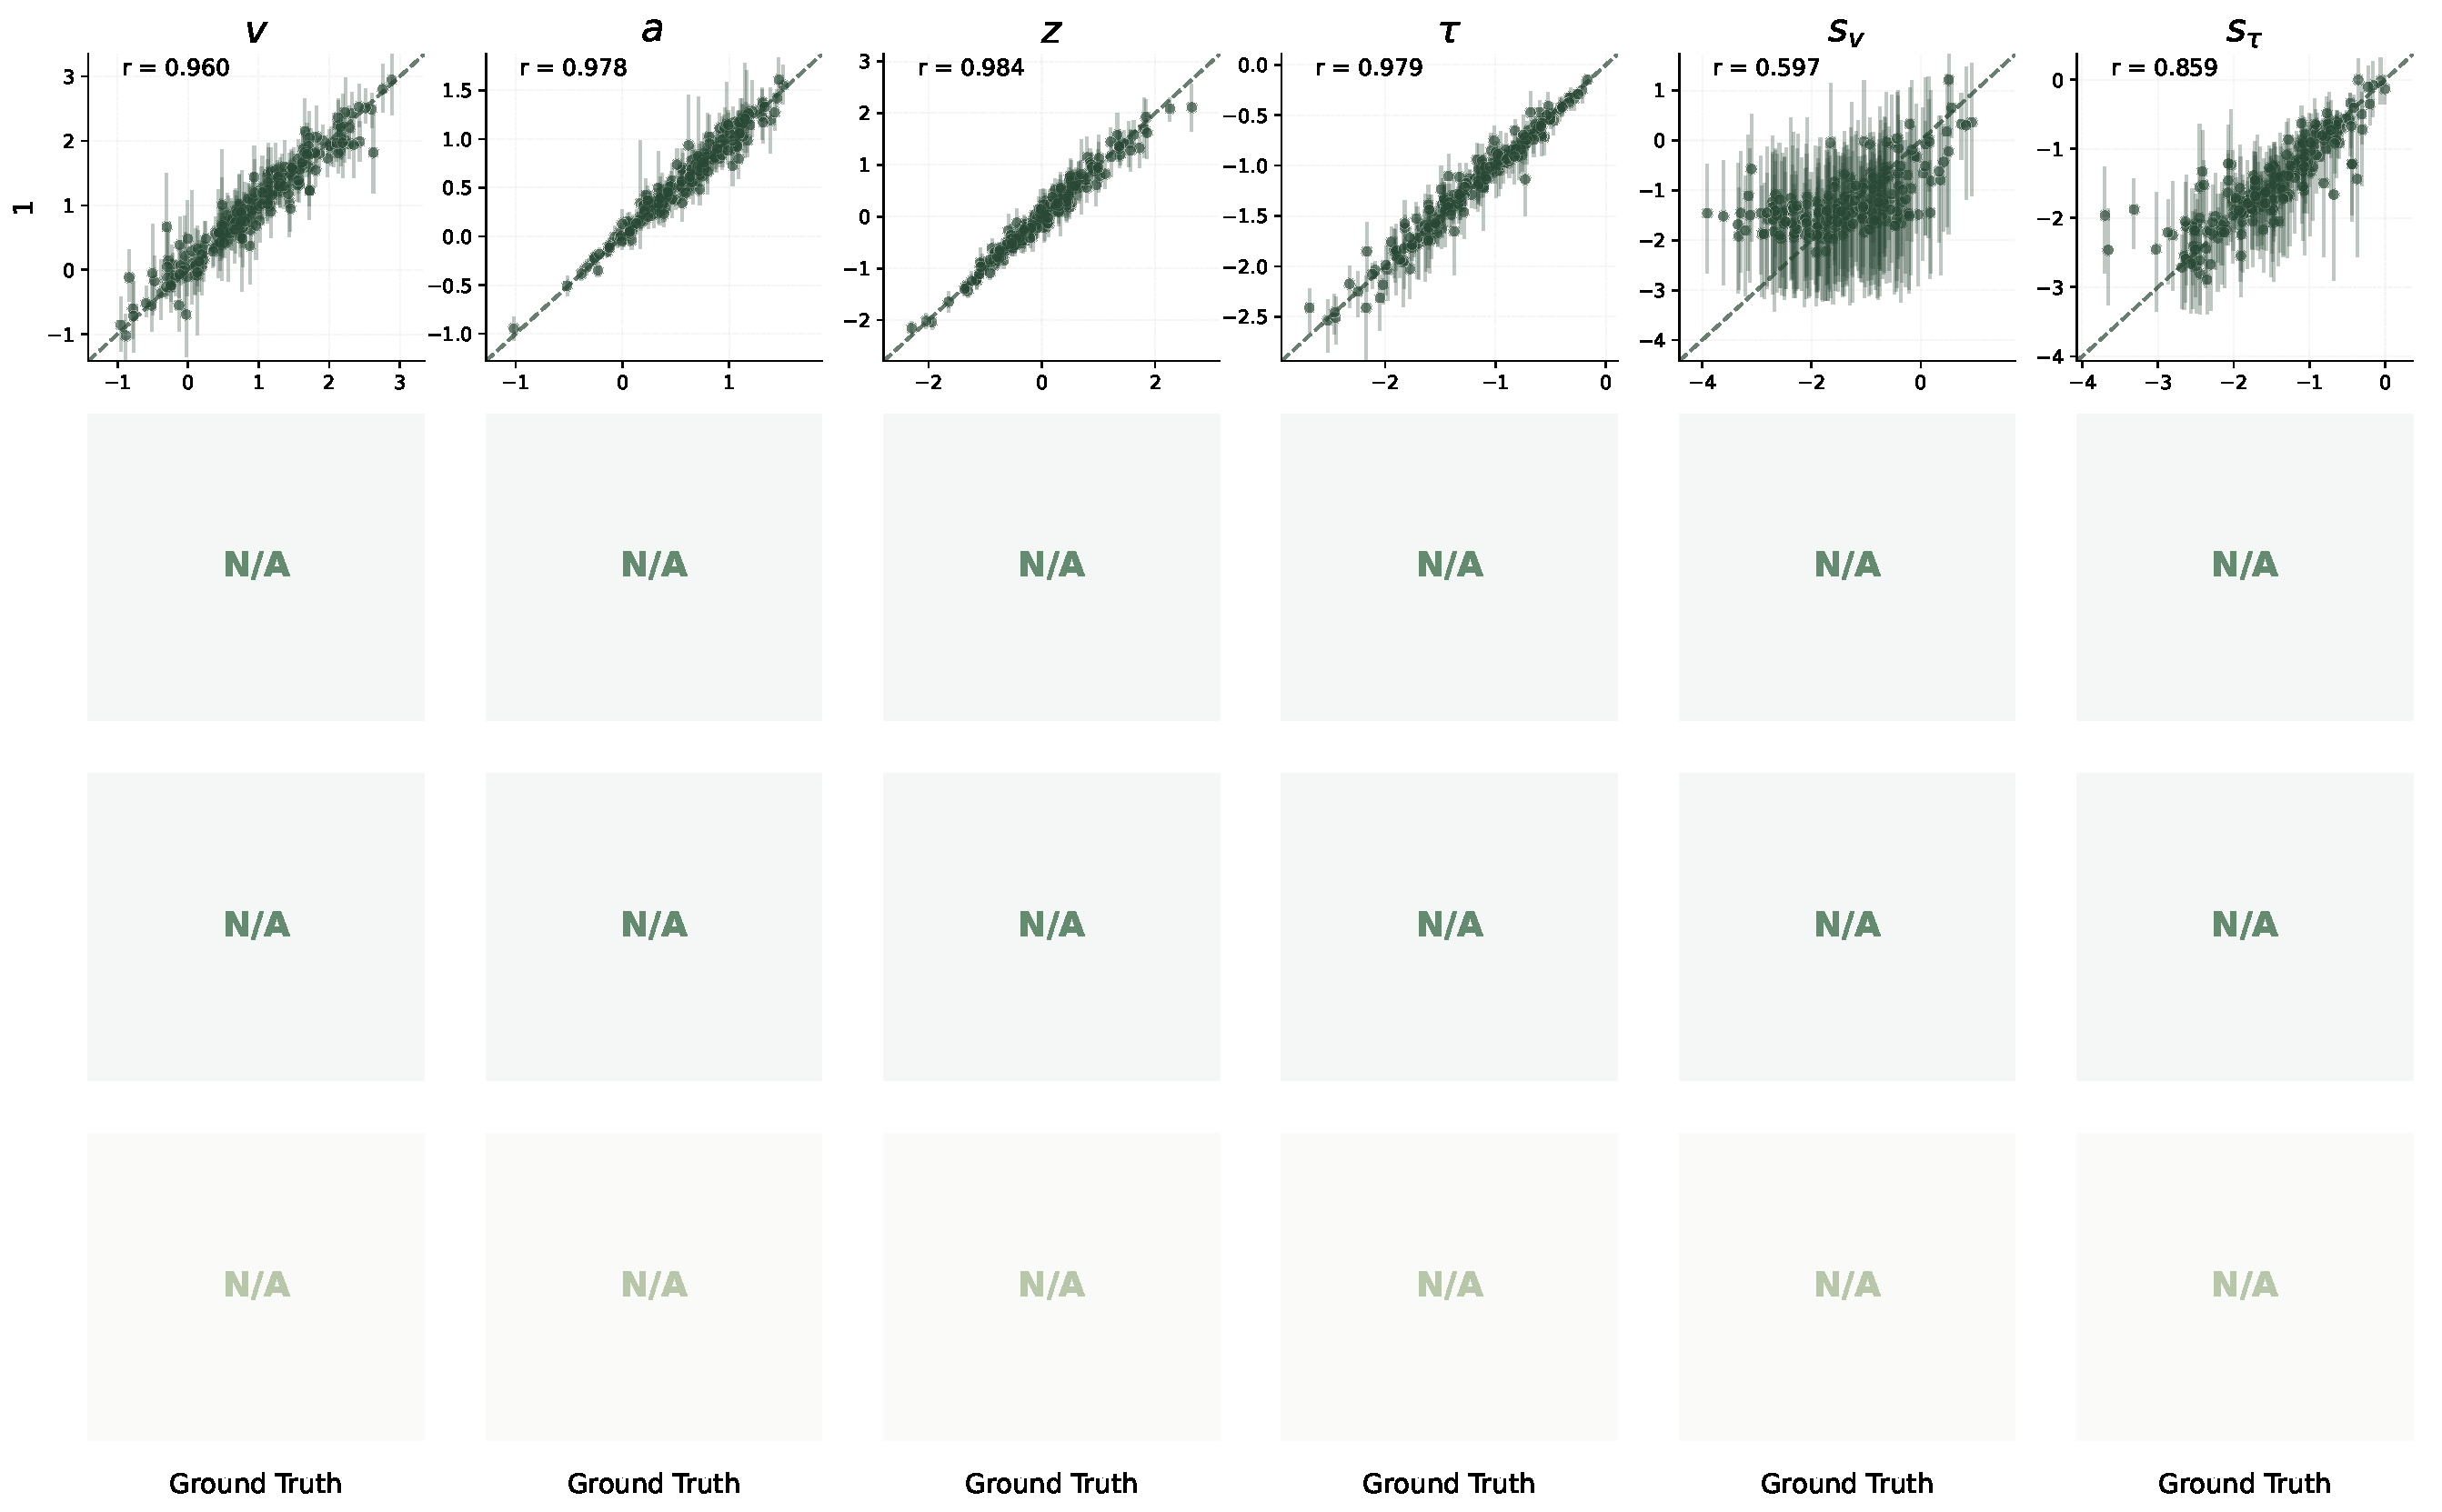
\includegraphics[width=0.99\linewidth]{figures/bf/ddm/intercept_only/ddm_family_intercept_only_bf_recovery.pdf}
    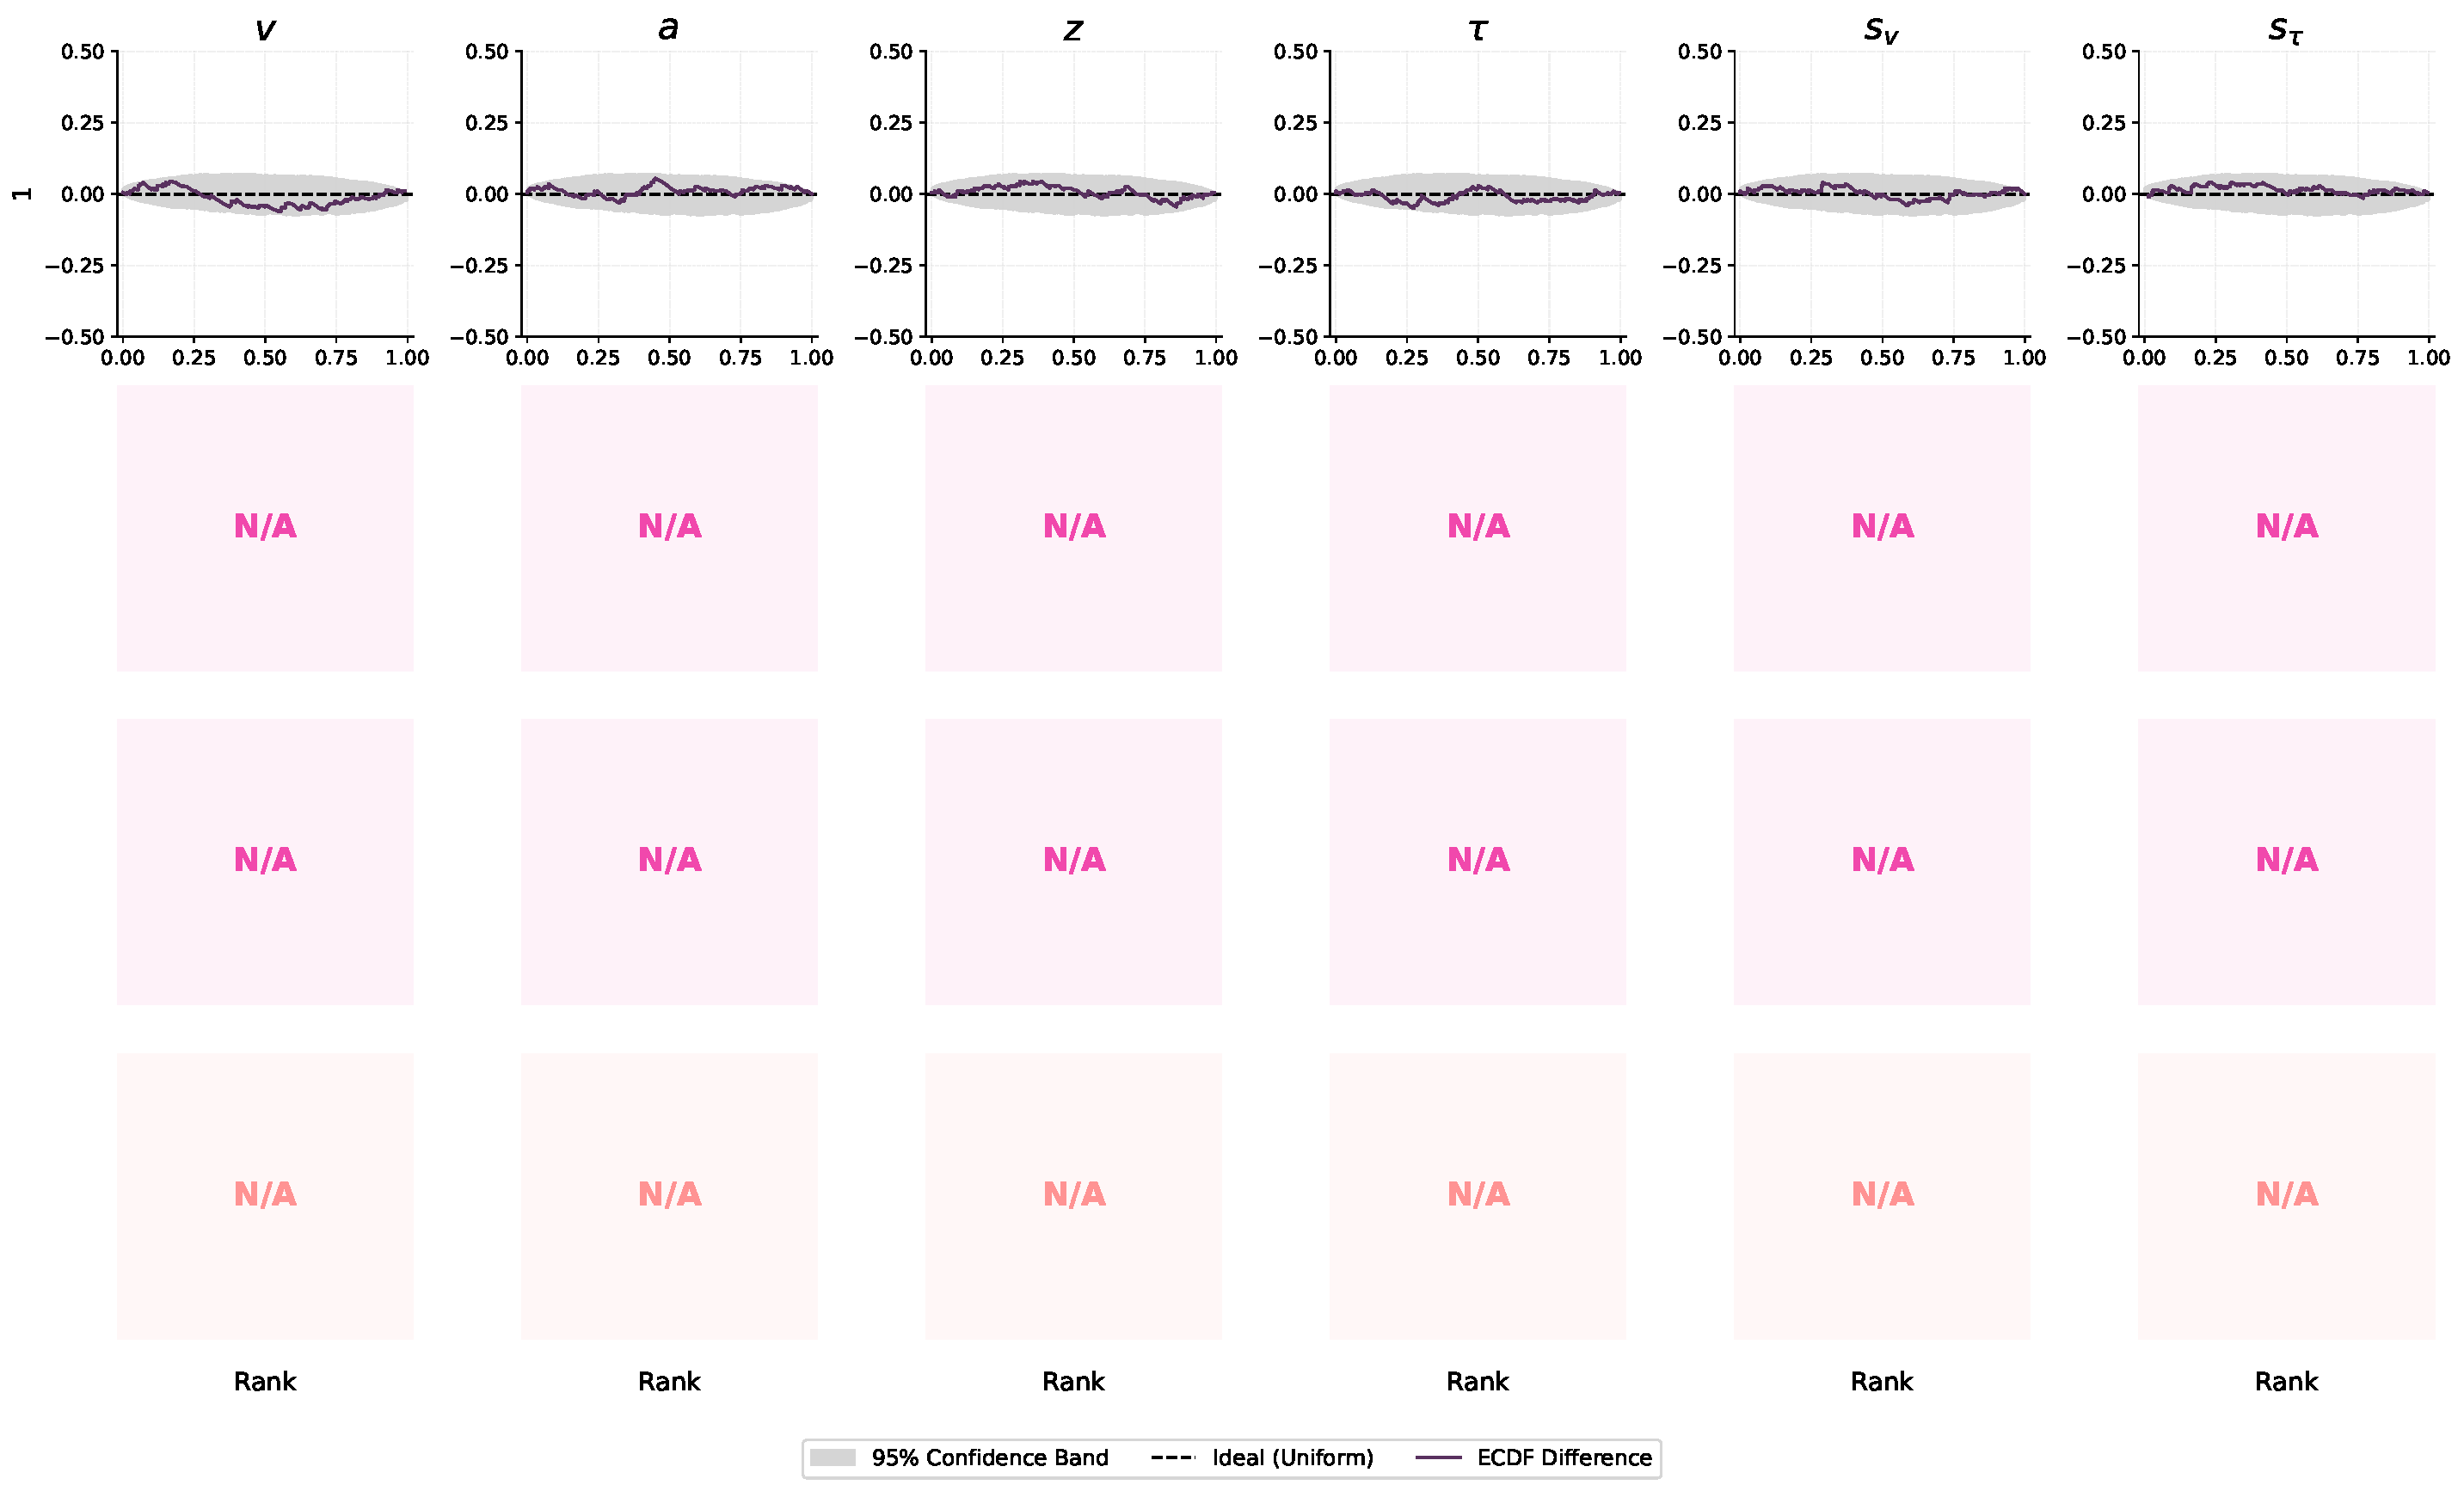
\includegraphics[width=0.99\linewidth]{figures/bf/ddm/intercept_only/ddm_family_intercept_only_bf_ecdf.pdf}
    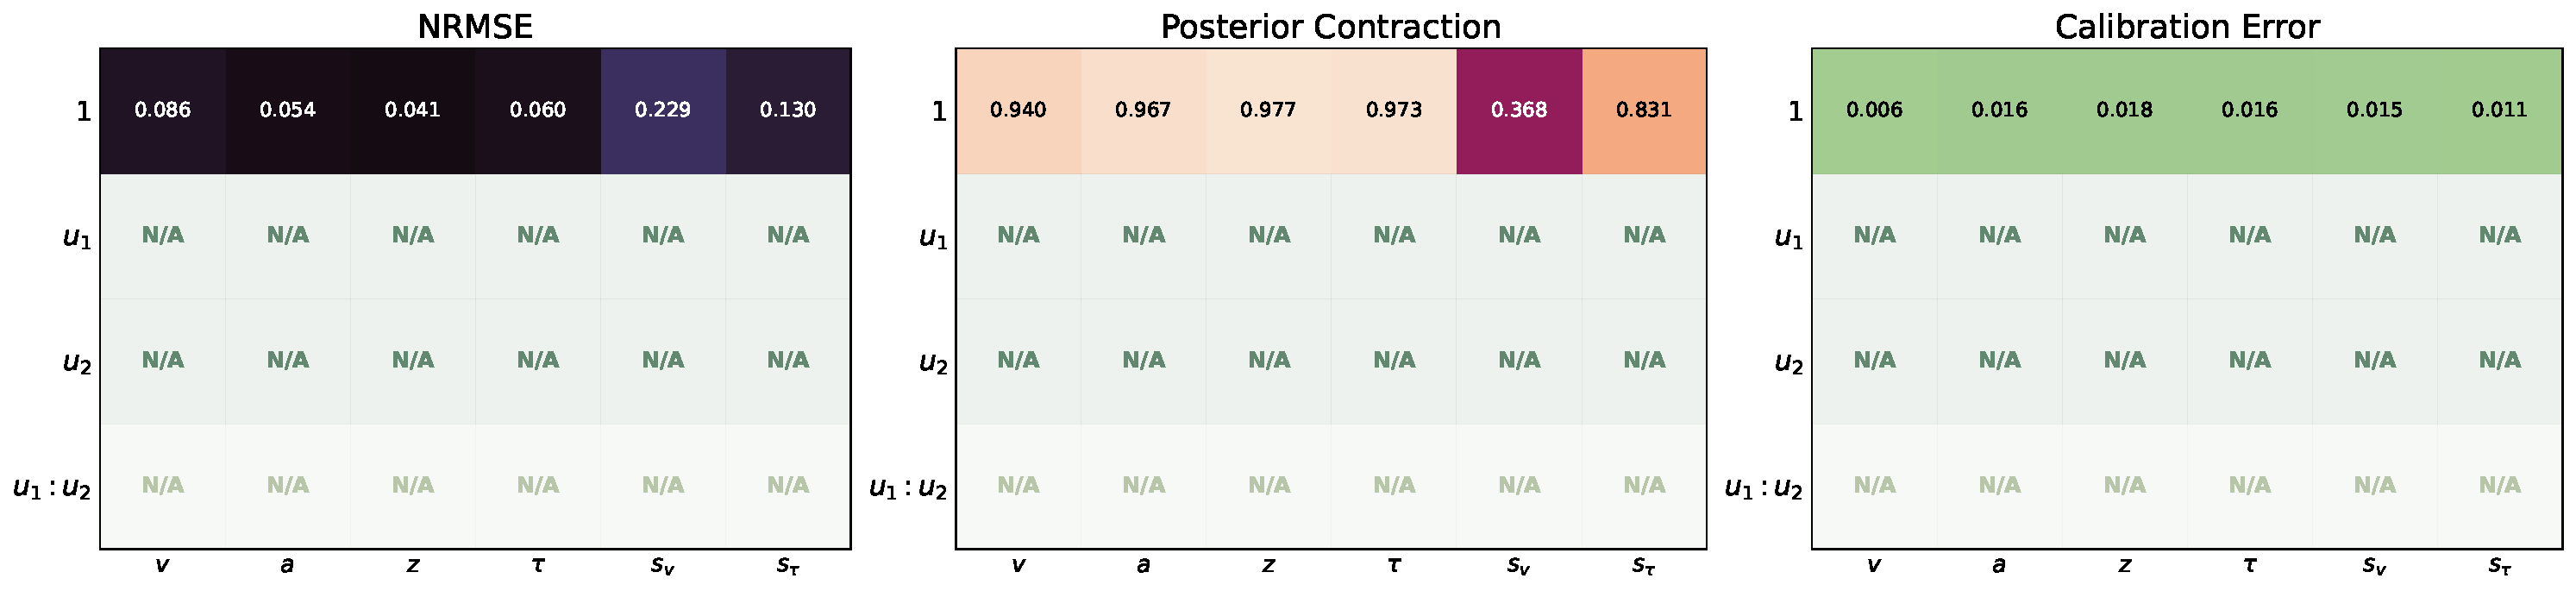
\includegraphics[width=0.99\linewidth]{figures/bf/ddm/intercept_only/ddm_family_intercept_only_bf_metrics.pdf}
    \caption{Parameter recovery (\emph{top}), calibration ECDF (\emph{middle}), and parameter-wise metrics (NRMSE, calibration error, and posterior contraction) for DDM baseline (Case \textbf{intercept\_only}).}
    \label{fig:ddm-bf-intercept-only}
\end{figure}

\begin{figure}
    \centering
    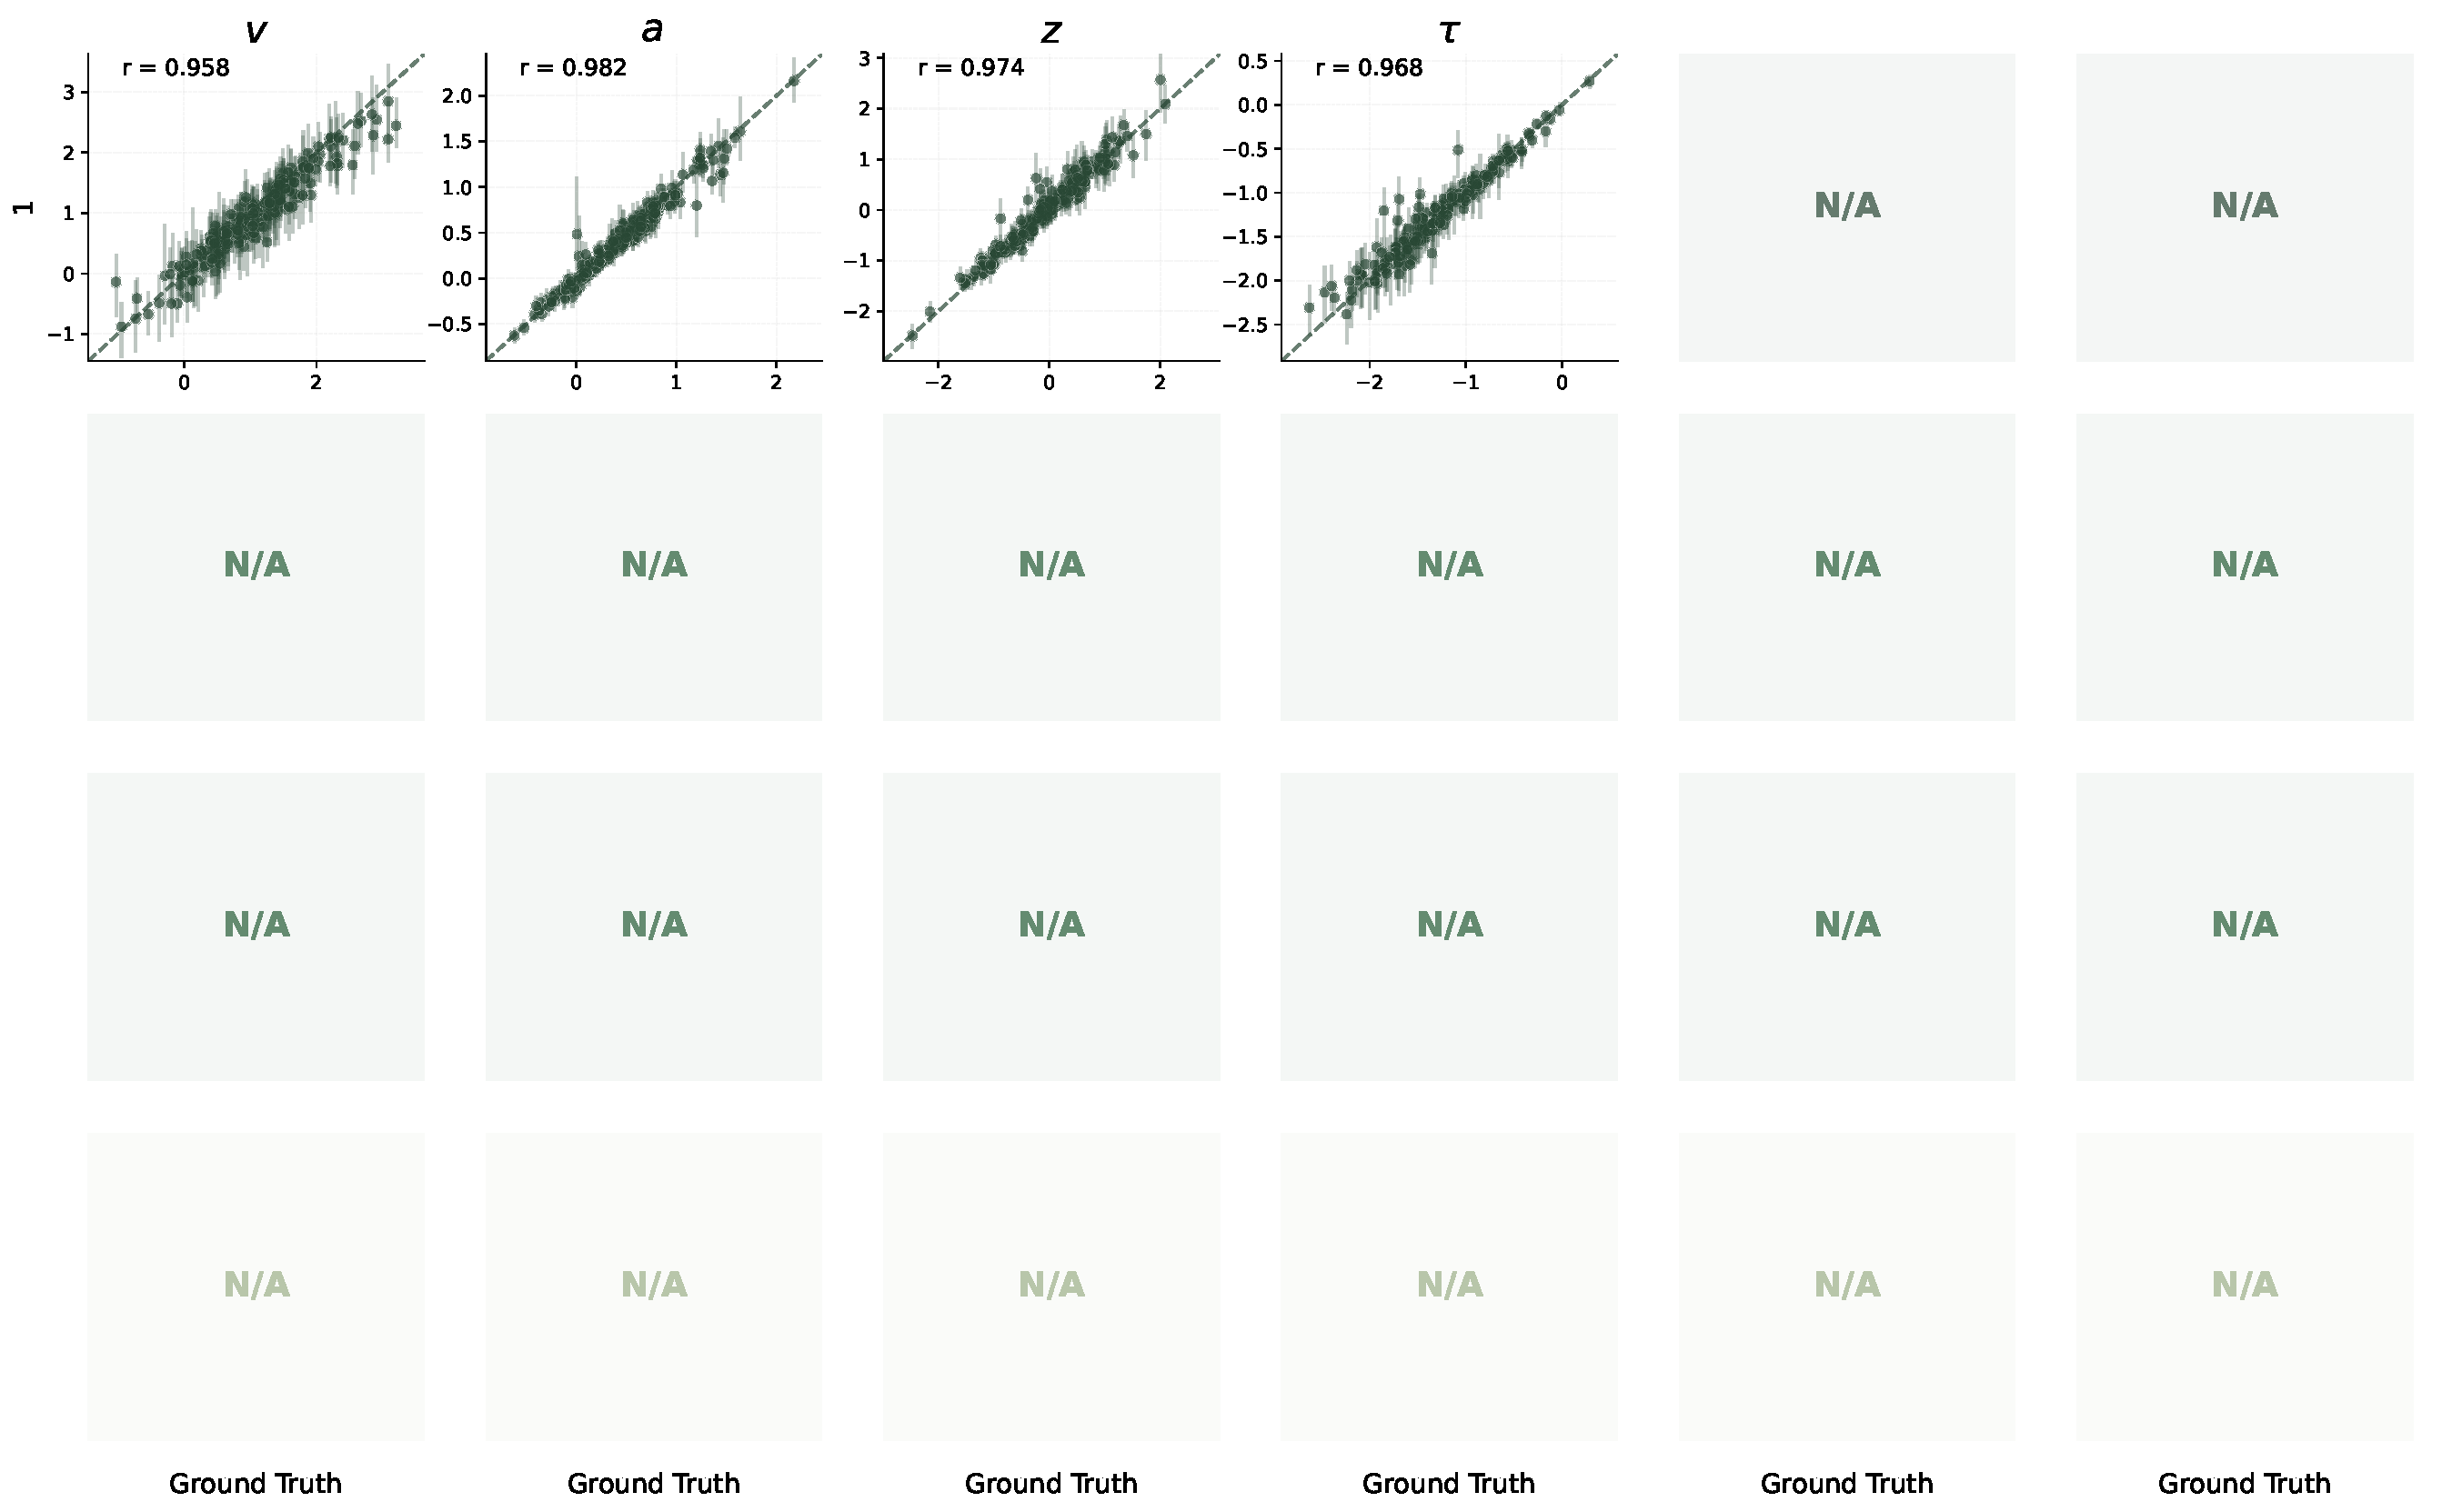
\includegraphics[width=0.99\linewidth]{figures/bf/ddm/fixed/ddm_family_fixed_bf_recovery.pdf}
    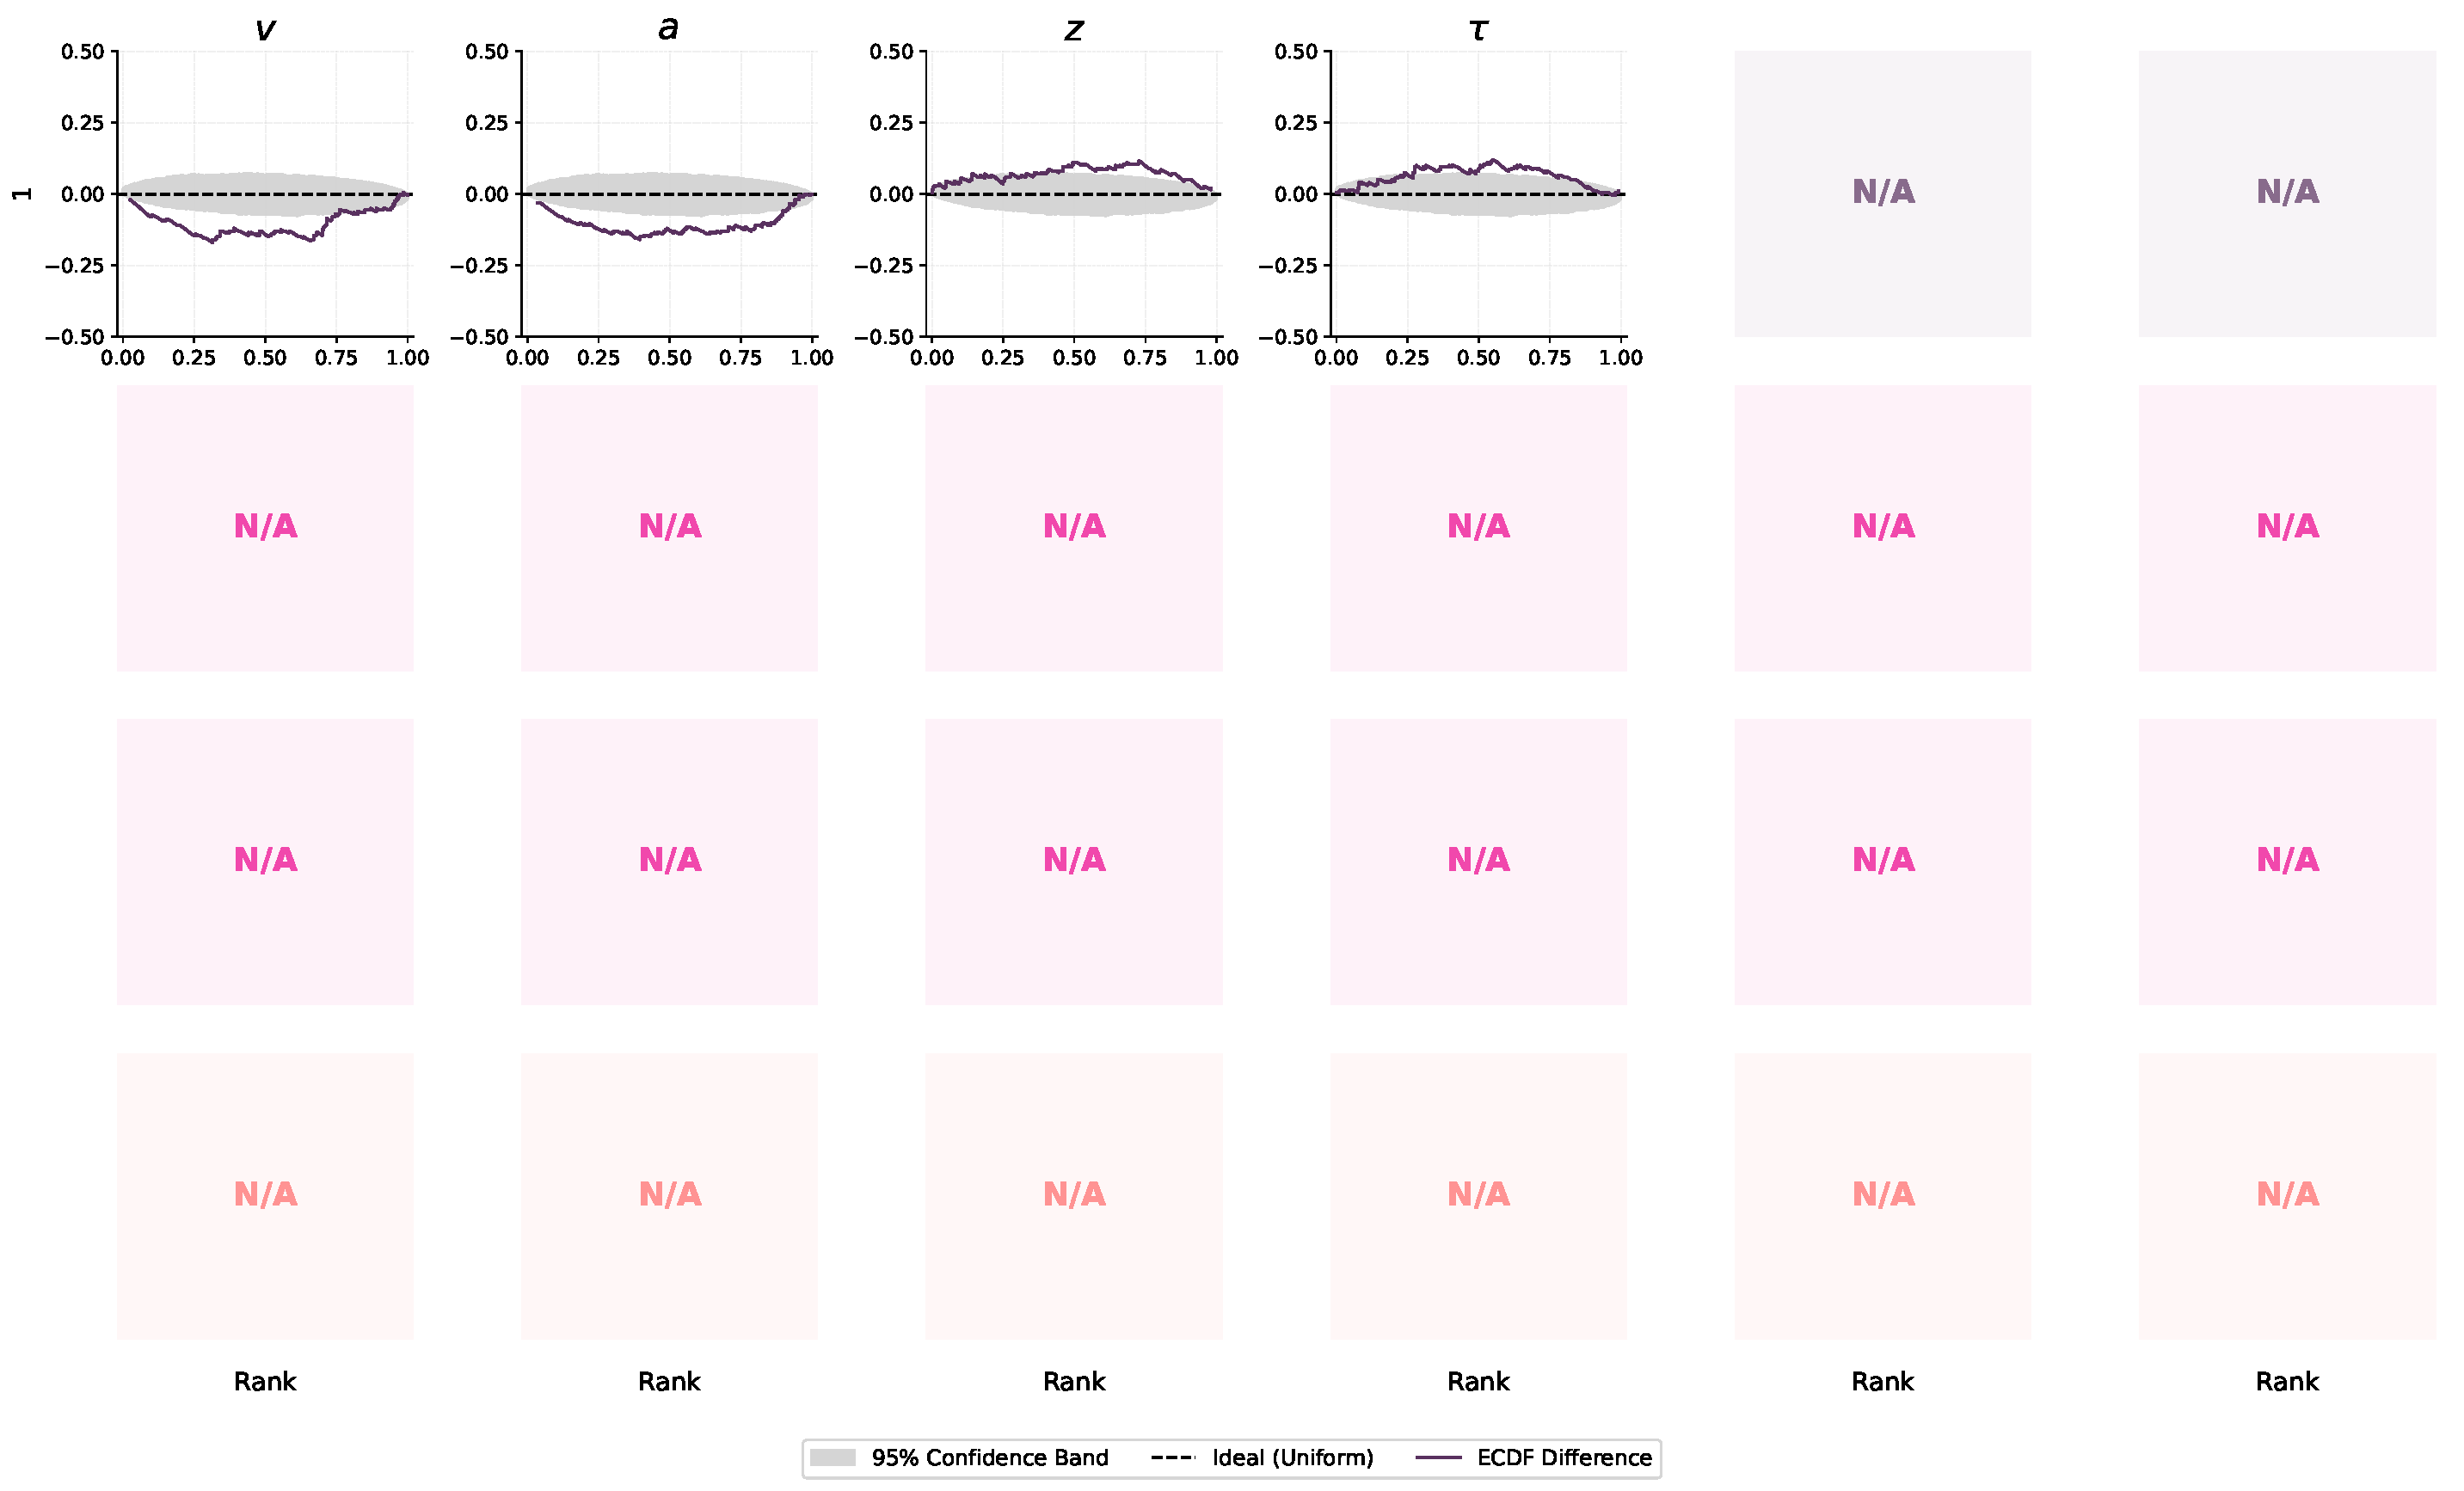
\includegraphics[width=0.99\linewidth]{figures/bf/ddm/fixed/ddm_family_fixed_bf_ecdf.pdf}
    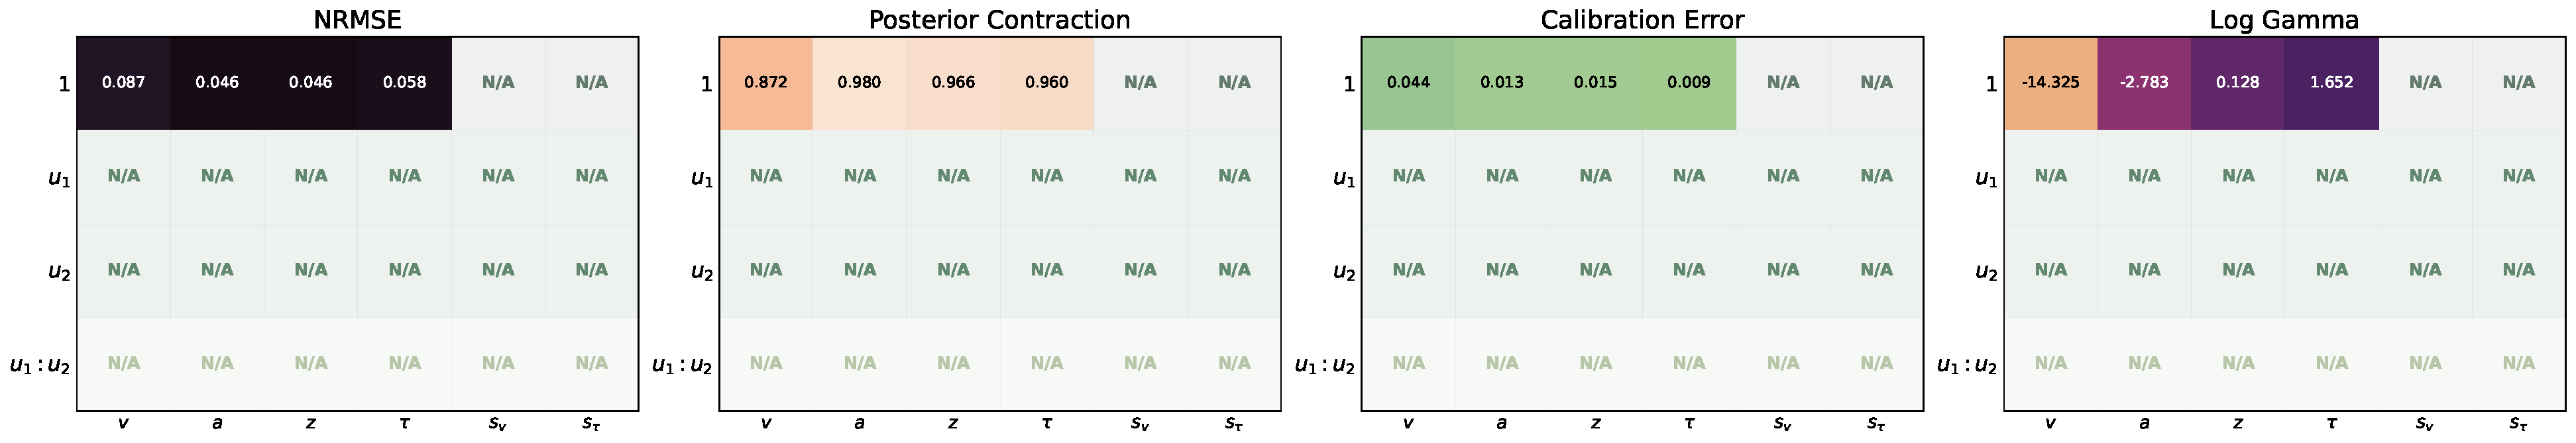
\includegraphics[width=0.99\linewidth]{figures/bf/ddm/fixed/ddm_family_fixed_bf_metrics.pdf}
    \caption{Parameter recovery (\emph{top}), calibration ECDF (\emph{middle}), and parameter-wise metrics (NRMSE, calibration error, and posterior contraction) for DDM baseline (Case \textbf{fixed}).}
    \label{fig:ddm-bf-fixed}
\end{figure}

\begin{figure}
    \centering
    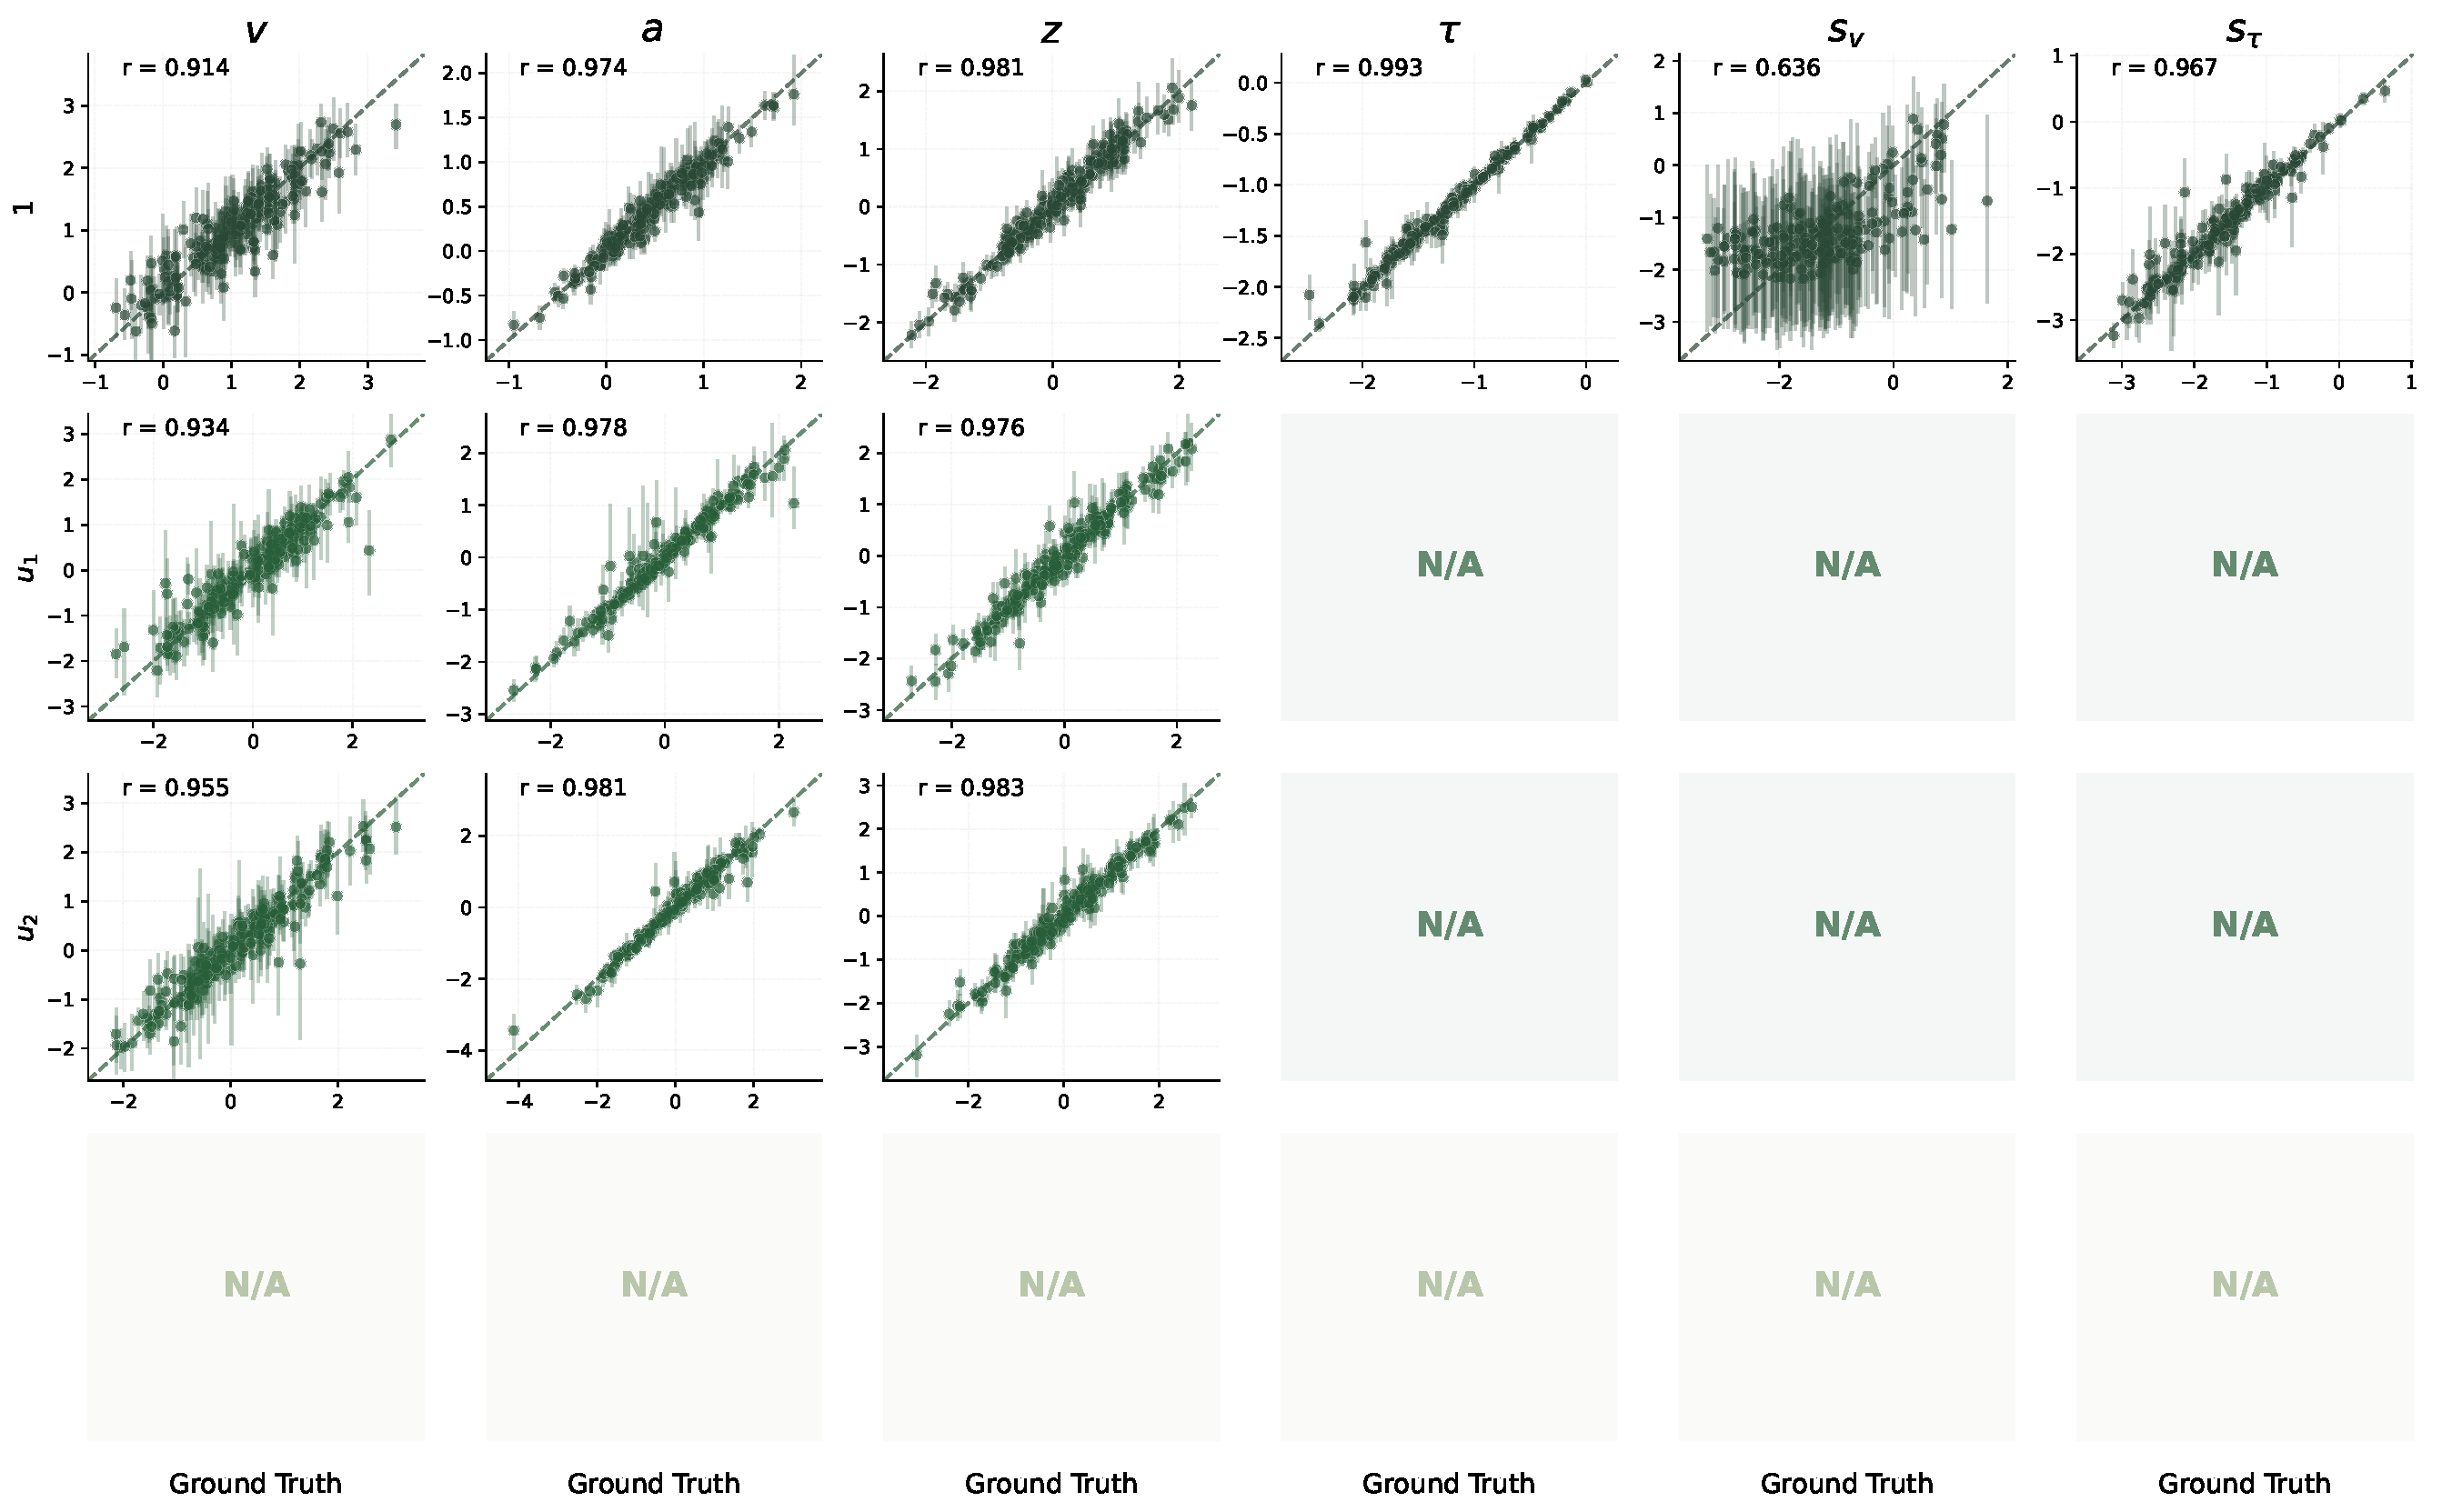
\includegraphics[width=0.99\linewidth]{figures/bf/ddm/regressed/ddm_family_regressed_bf_recovery.pdf}
    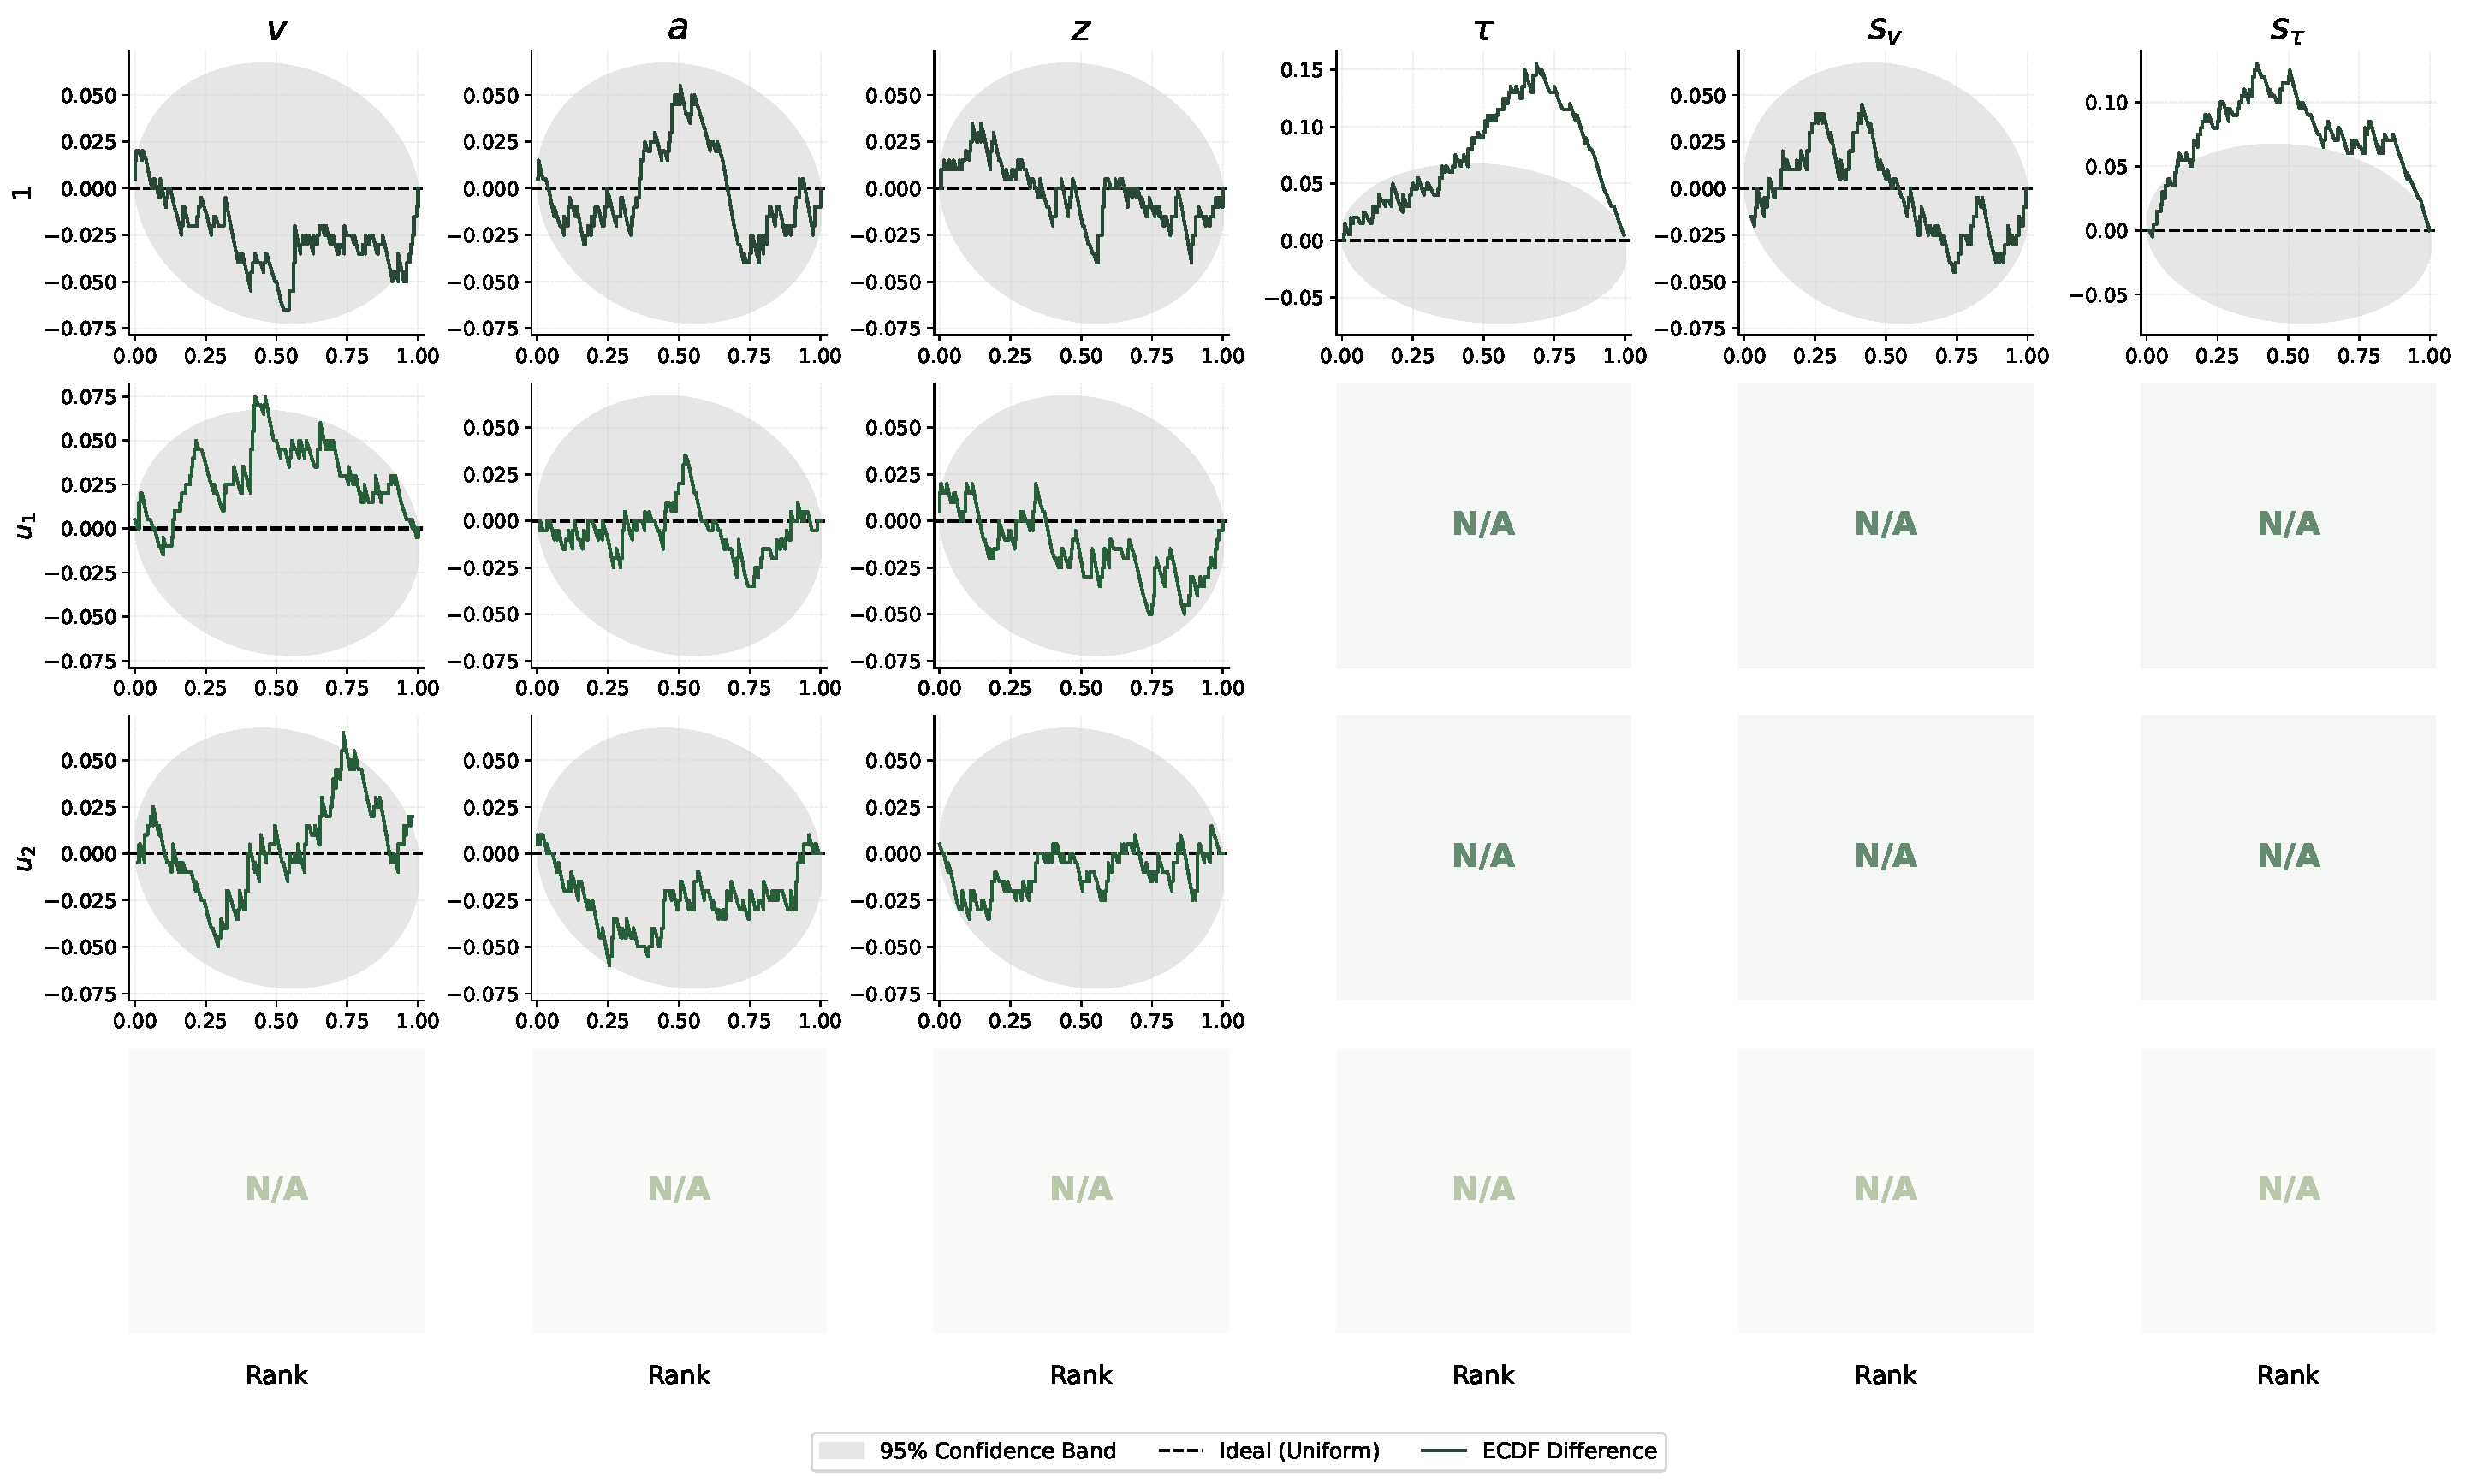
\includegraphics[width=0.99\linewidth]{figures/bf/ddm/regressed/ddm_family_regressed_bf_ecdf.pdf}
    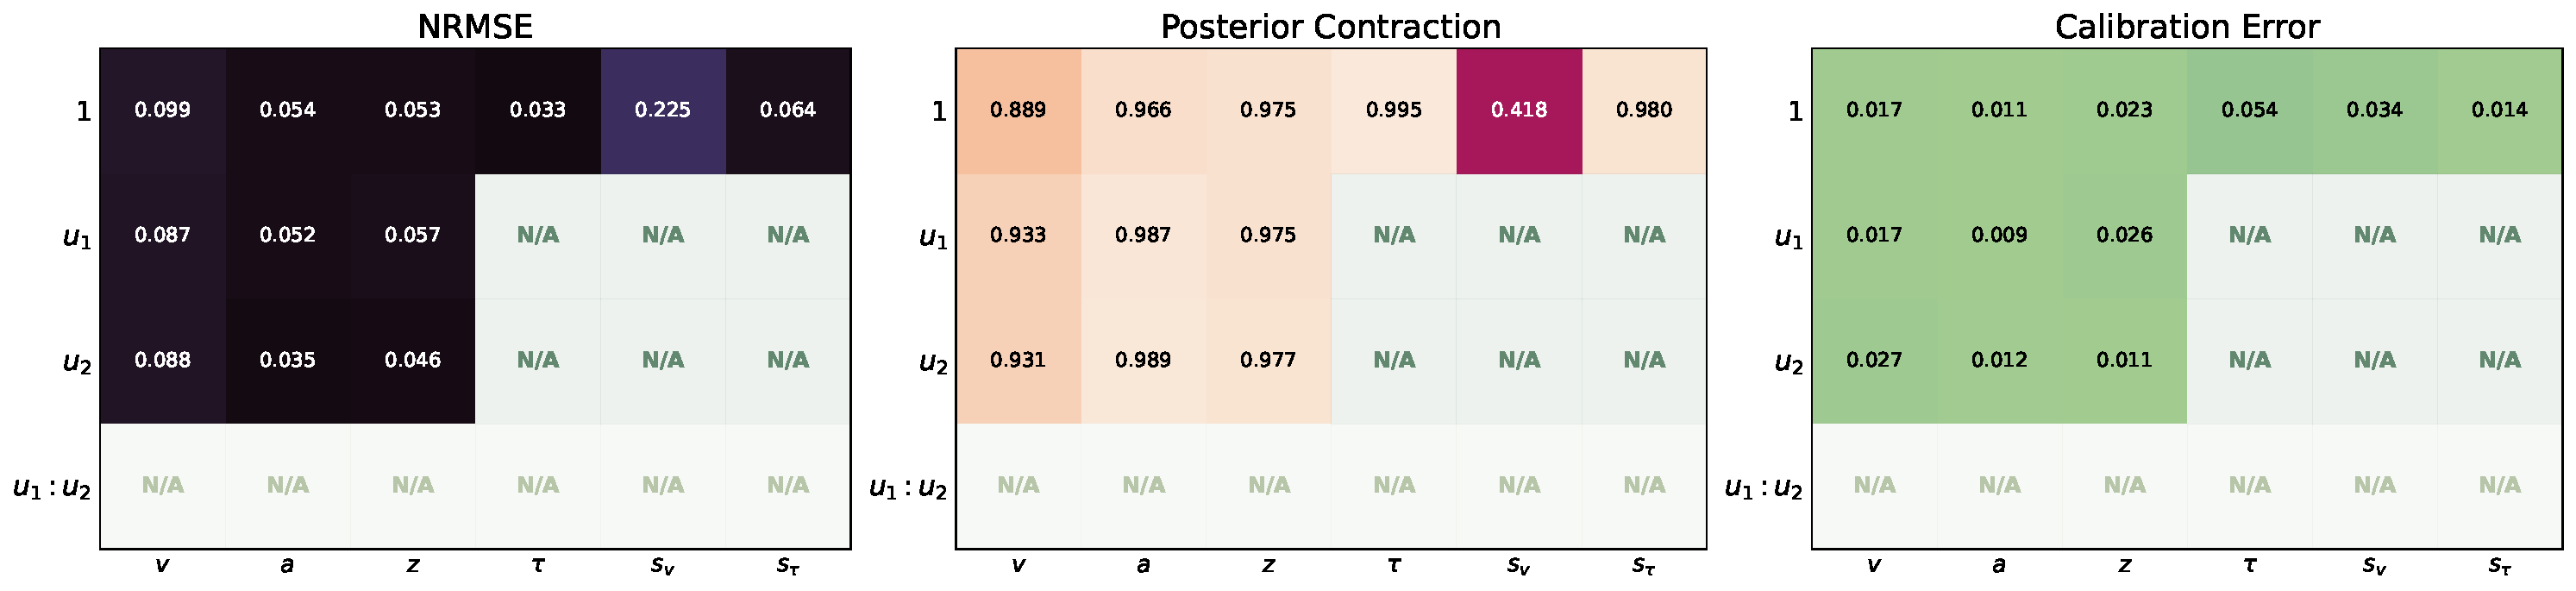
\includegraphics[width=0.99\linewidth]{figures/bf/ddm/regressed/ddm_family_regressed_bf_metrics.pdf}
    \caption{Parameter recovery (\emph{top}), calibration ECDF (\emph{middle}), and parameter-wise metrics (NRMSE, calibration error, and posterior contraction) for DDM baseline (Case \textbf{regressed}).}
    \label{fig:ddm-bf-regressed}
\end{figure}

\begin{figure}
    \centering
    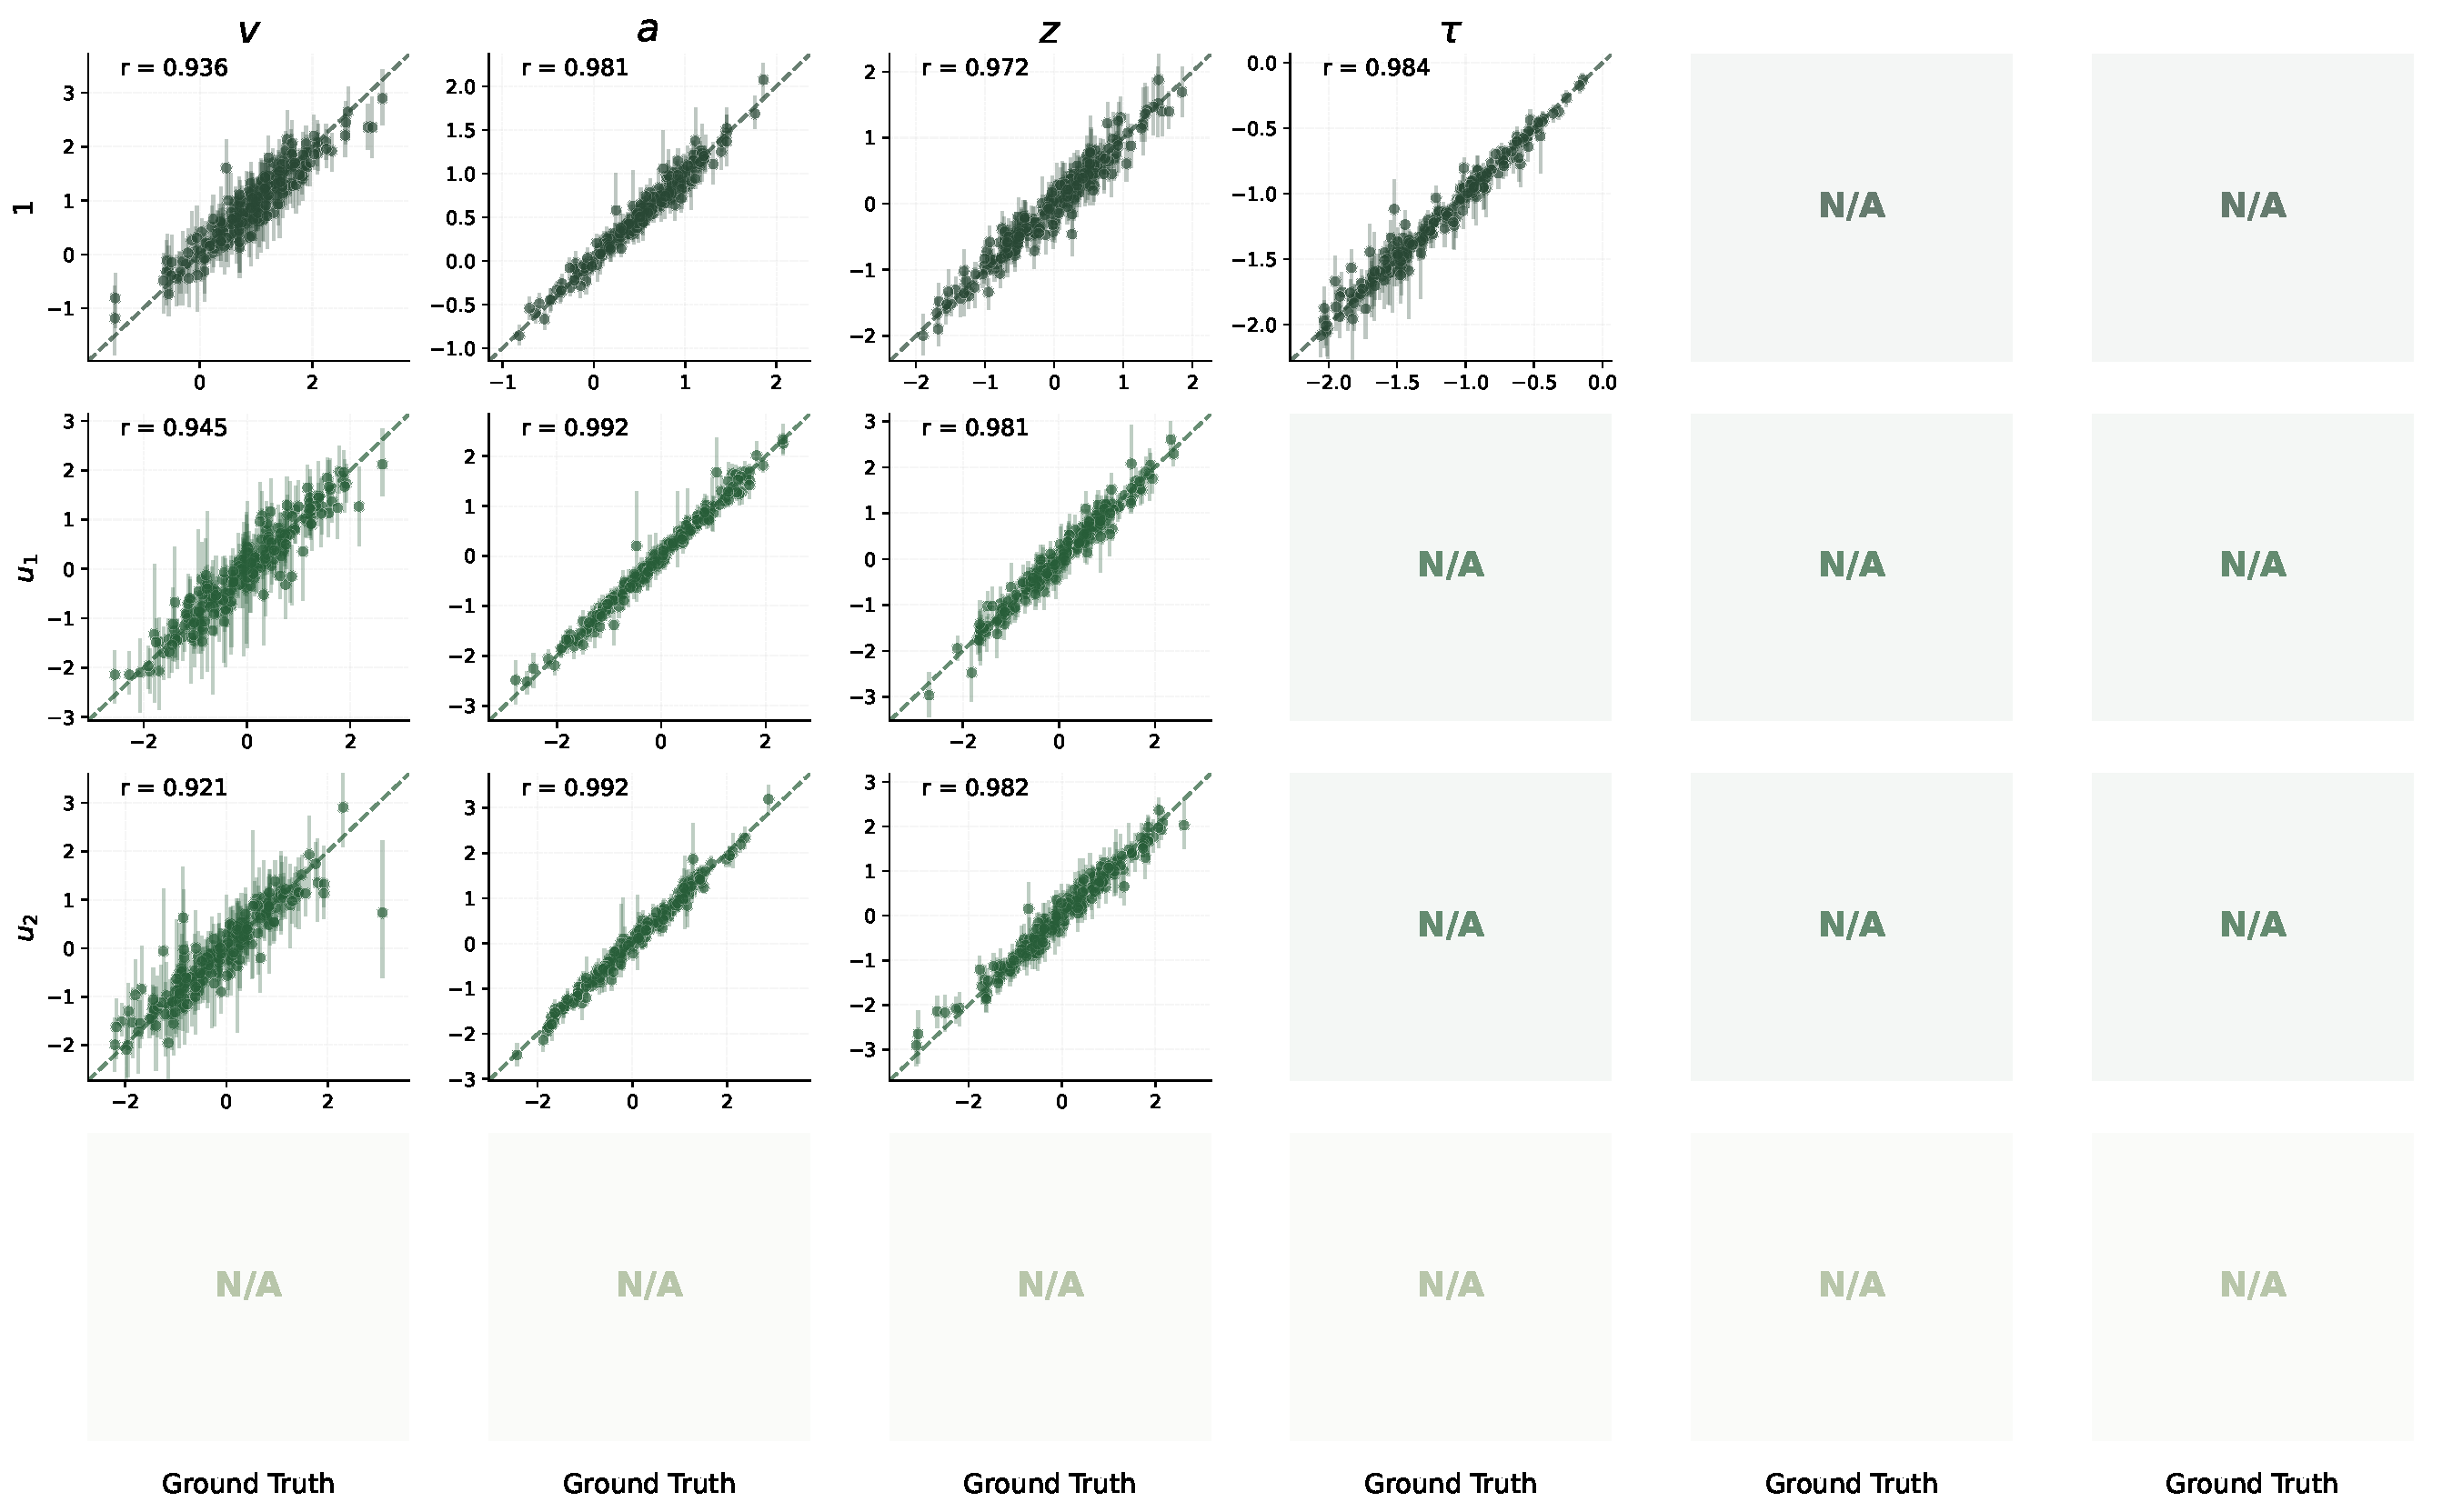
\includegraphics[width=0.99\linewidth]{figures/bf/ddm/fixed_regressed/ddm_family_fixed_regressed_bf_recovery.pdf}
    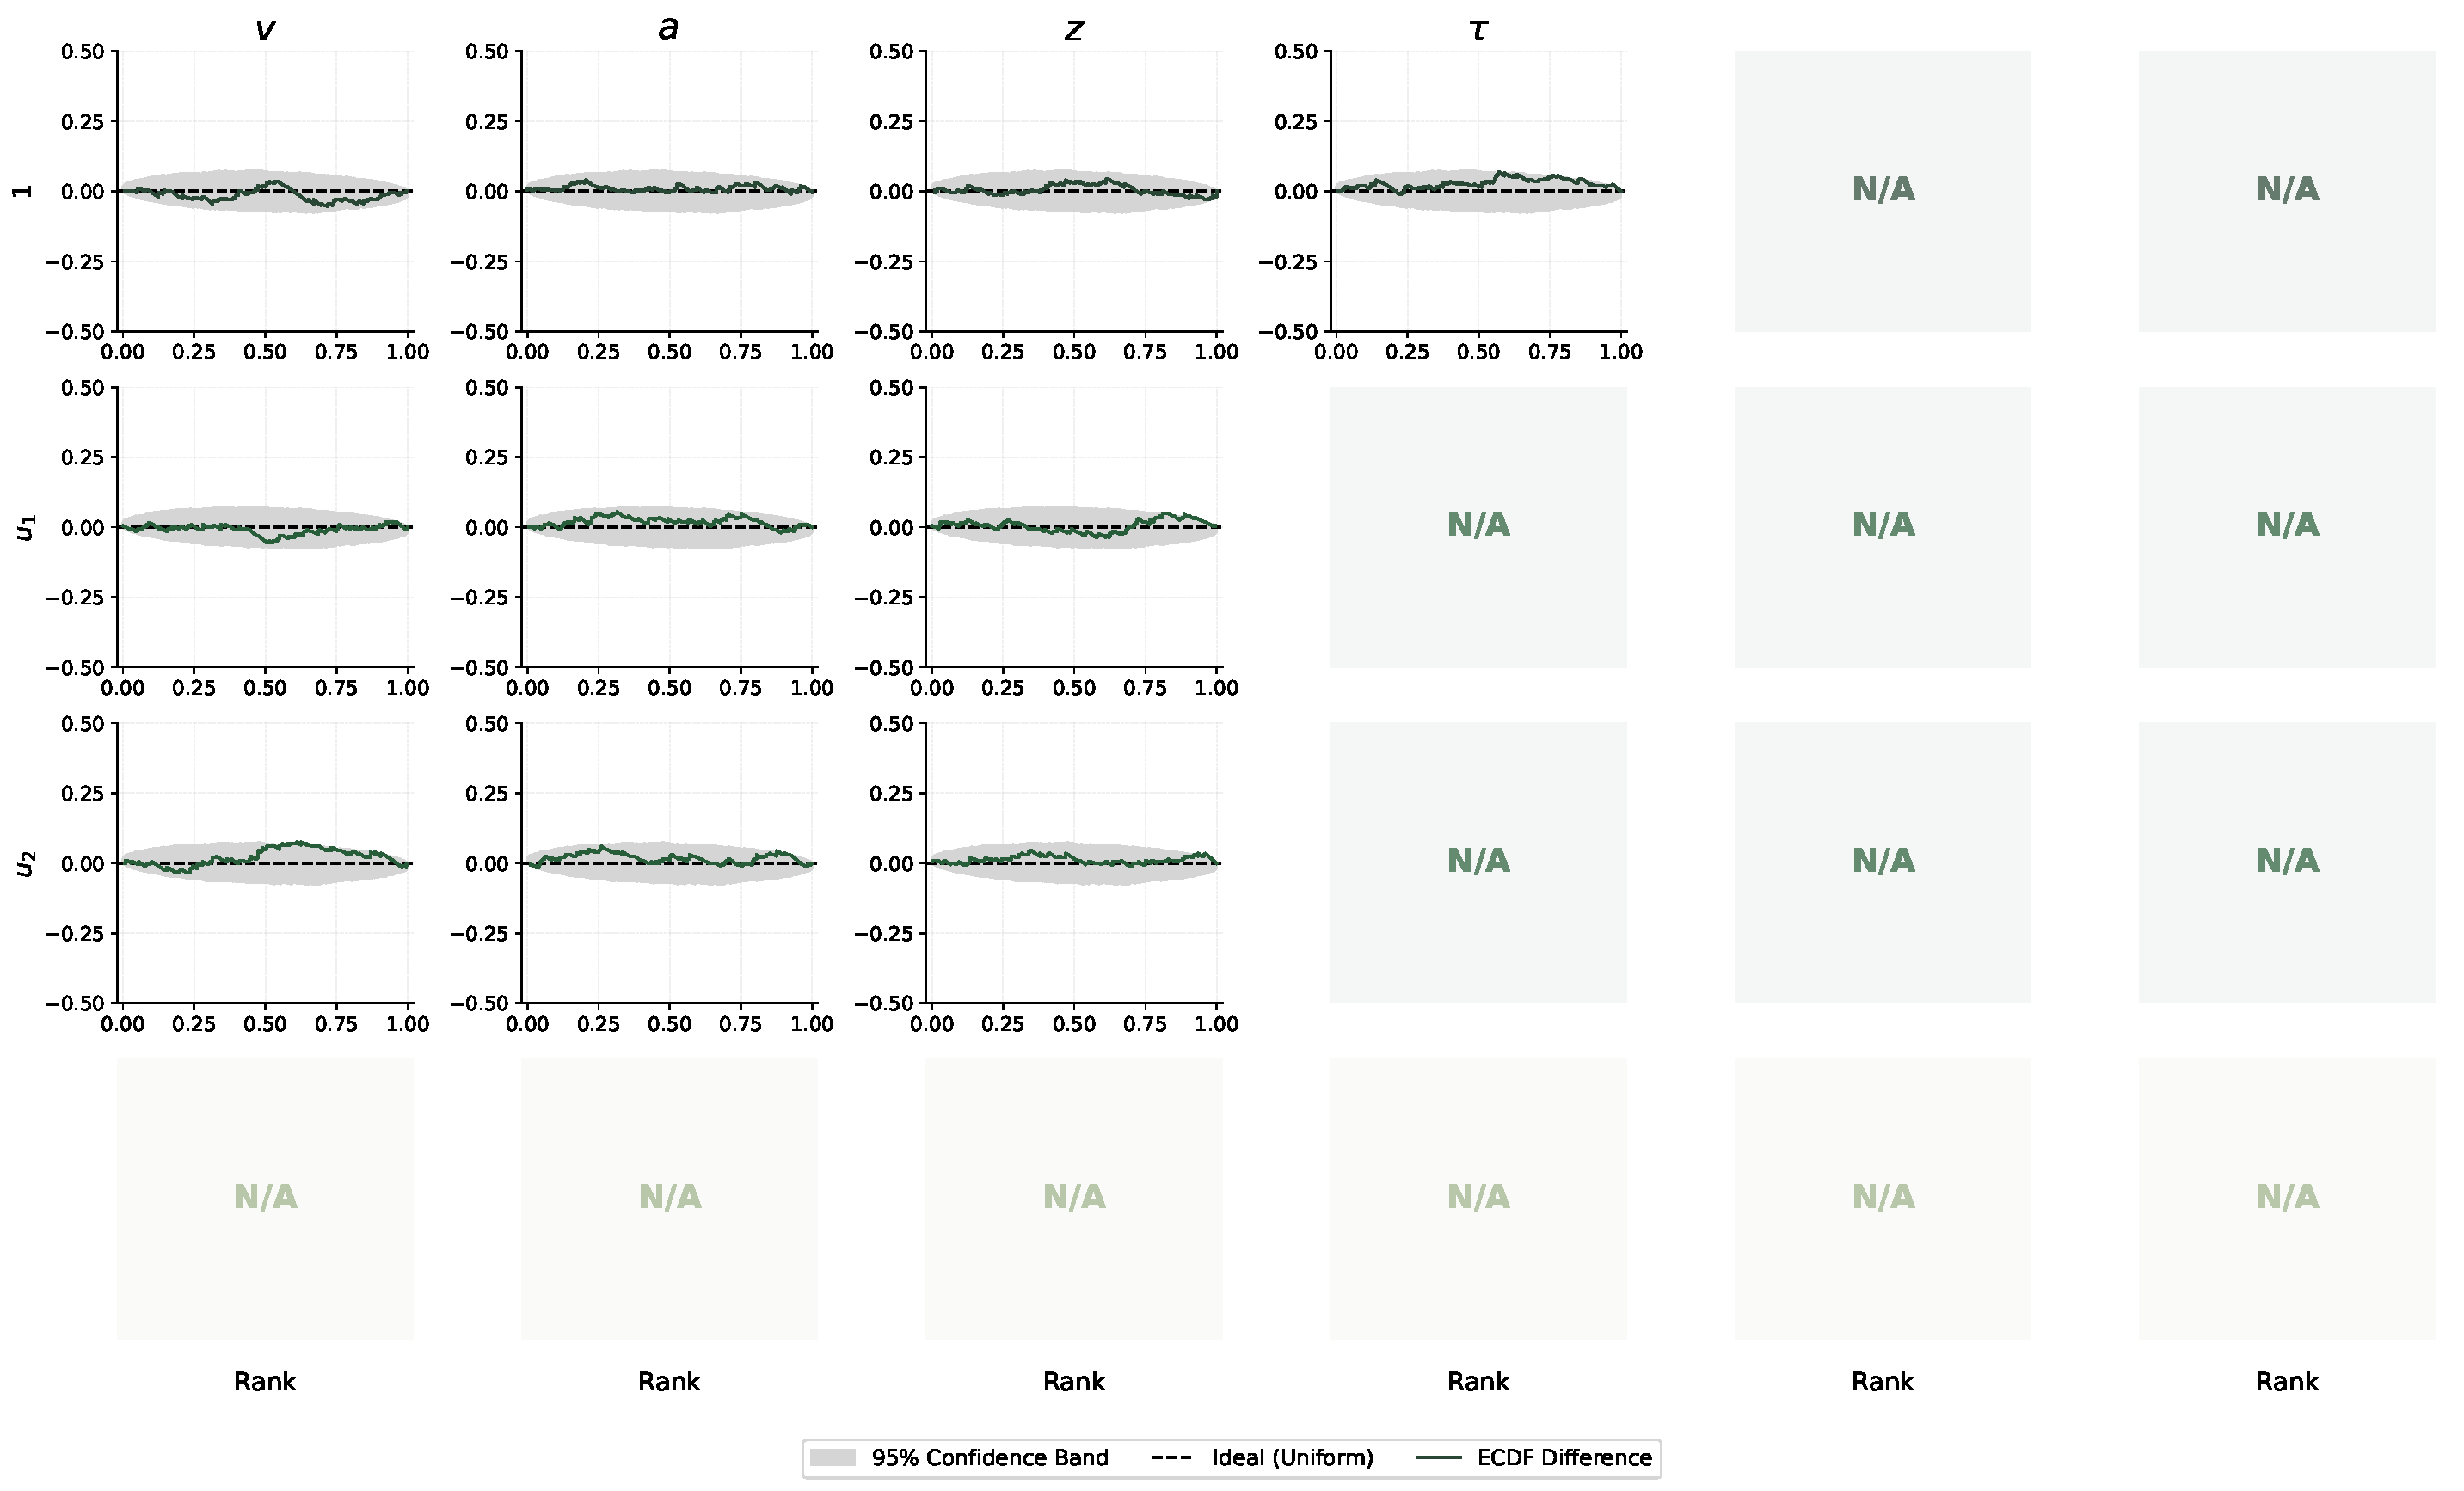
\includegraphics[width=0.99\linewidth]{figures/bf/ddm/fixed_regressed/ddm_family_fixed_regressed_bf_ecdf.pdf}
    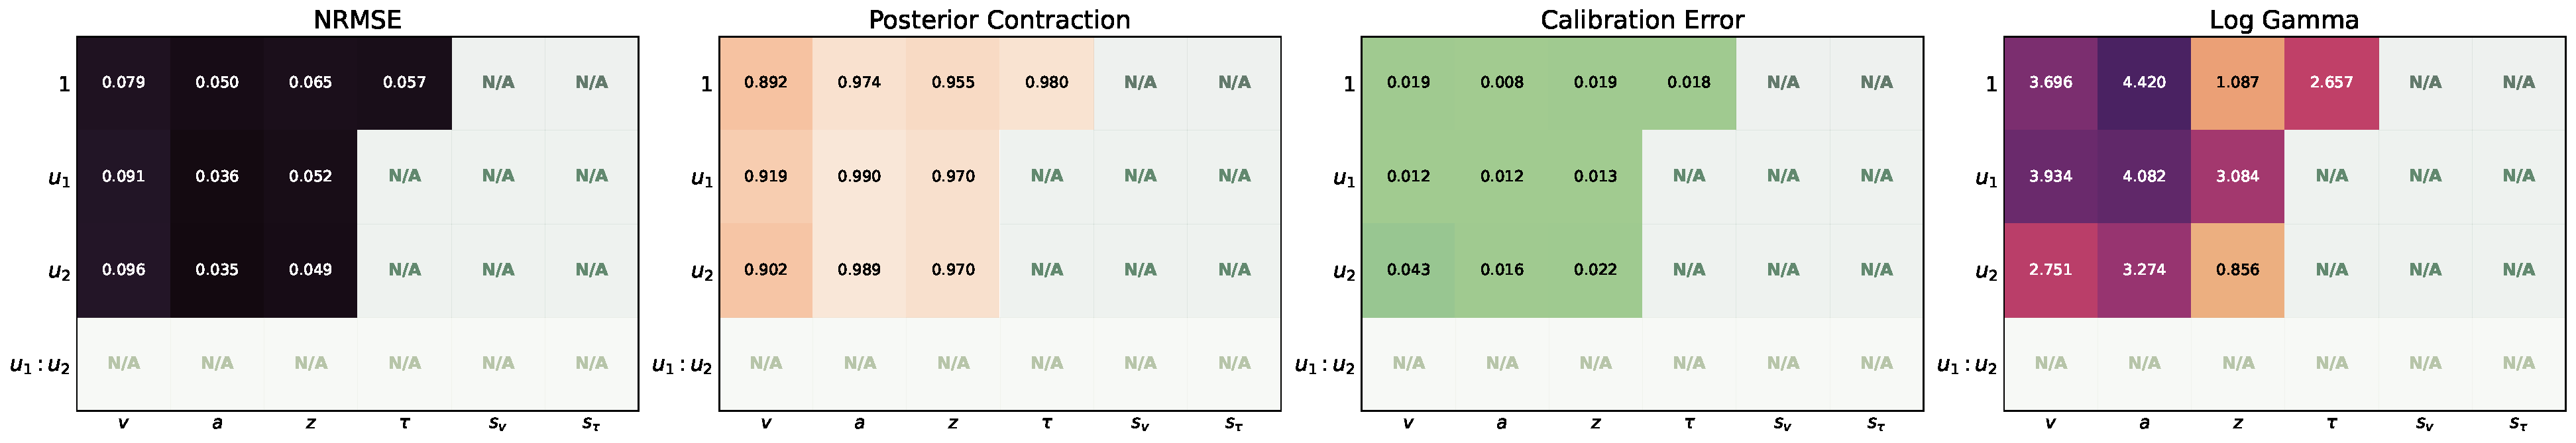
\includegraphics[width=0.99\linewidth]{figures/bf/ddm/fixed_regressed/ddm_family_fixed_regressed_bf_metrics.pdf}
    \caption{Parameter recovery (\emph{top}), calibration ECDF (\emph{middle}), and parameter-wise metrics (NRMSE, calibration error, and posterior contraction) for DDM baseline (Case \textbf{fixed\_regressed}).}
    \label{fig:ddm-bf-fixed-regressed}
\end{figure}

\begin{figure}
    \centering
    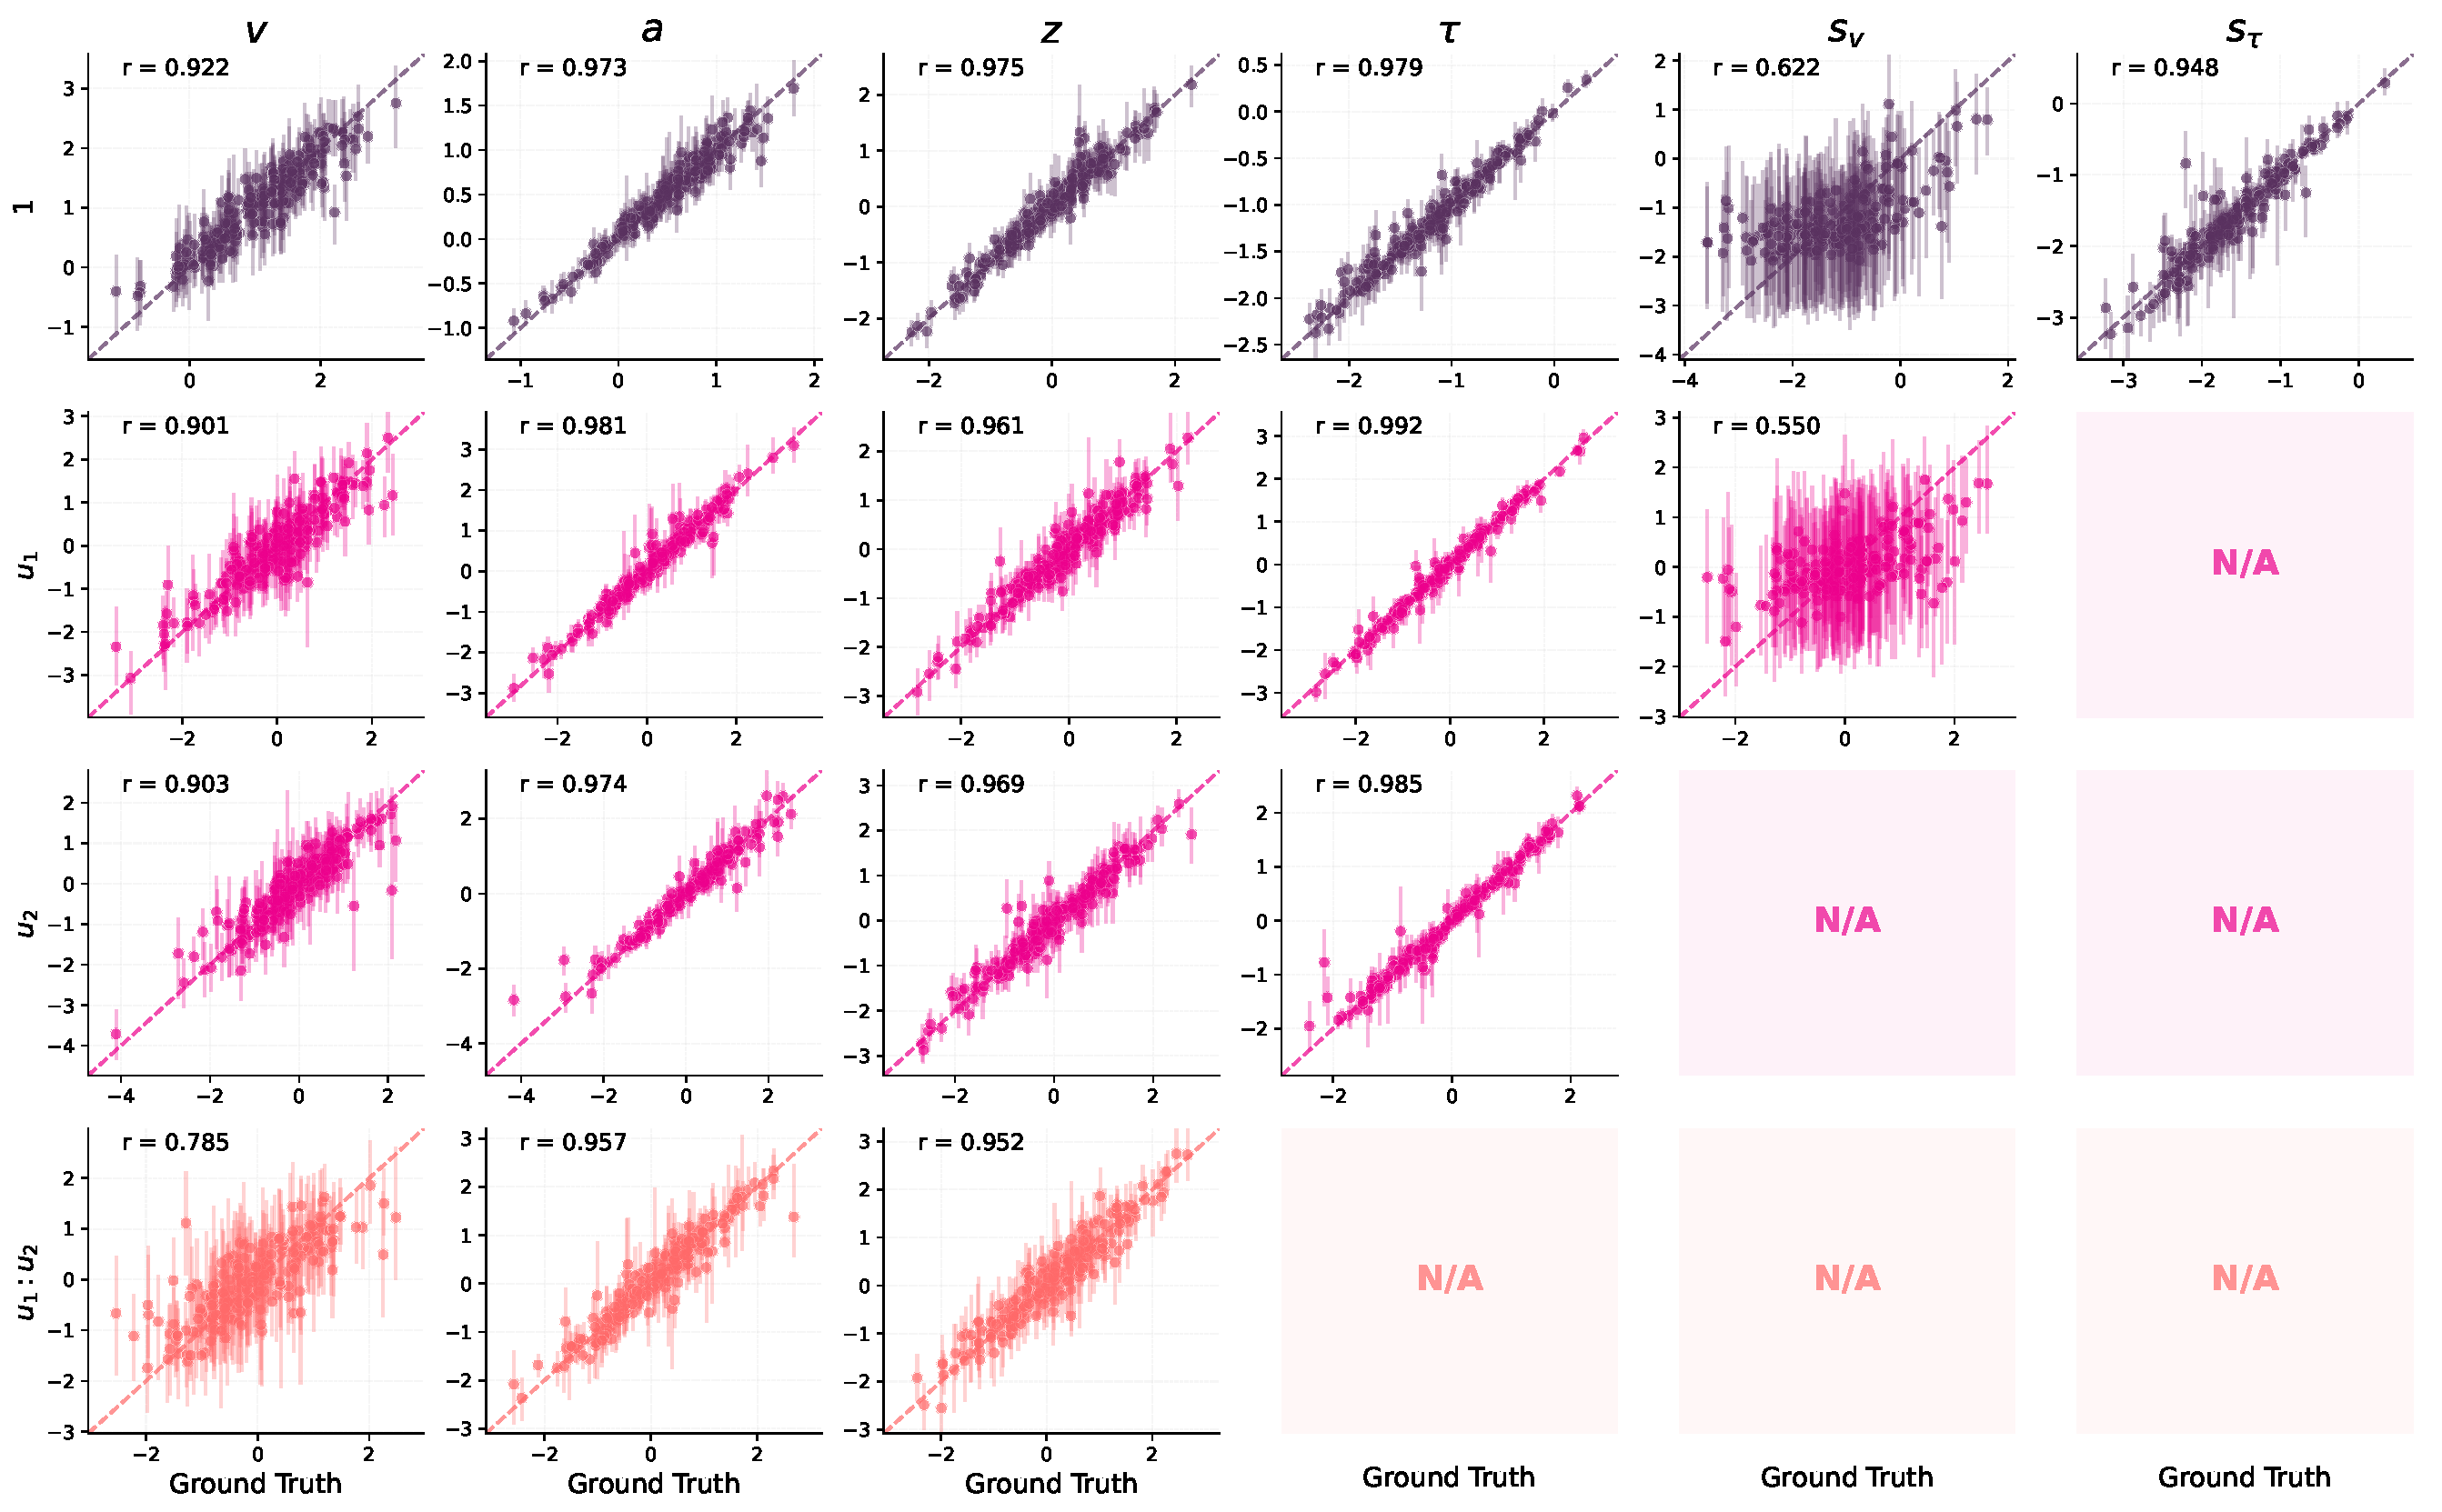
\includegraphics[width=0.99\linewidth]{figures/bf/ddm/interaction/ddm_family_interaction_bf_recovery.pdf}
    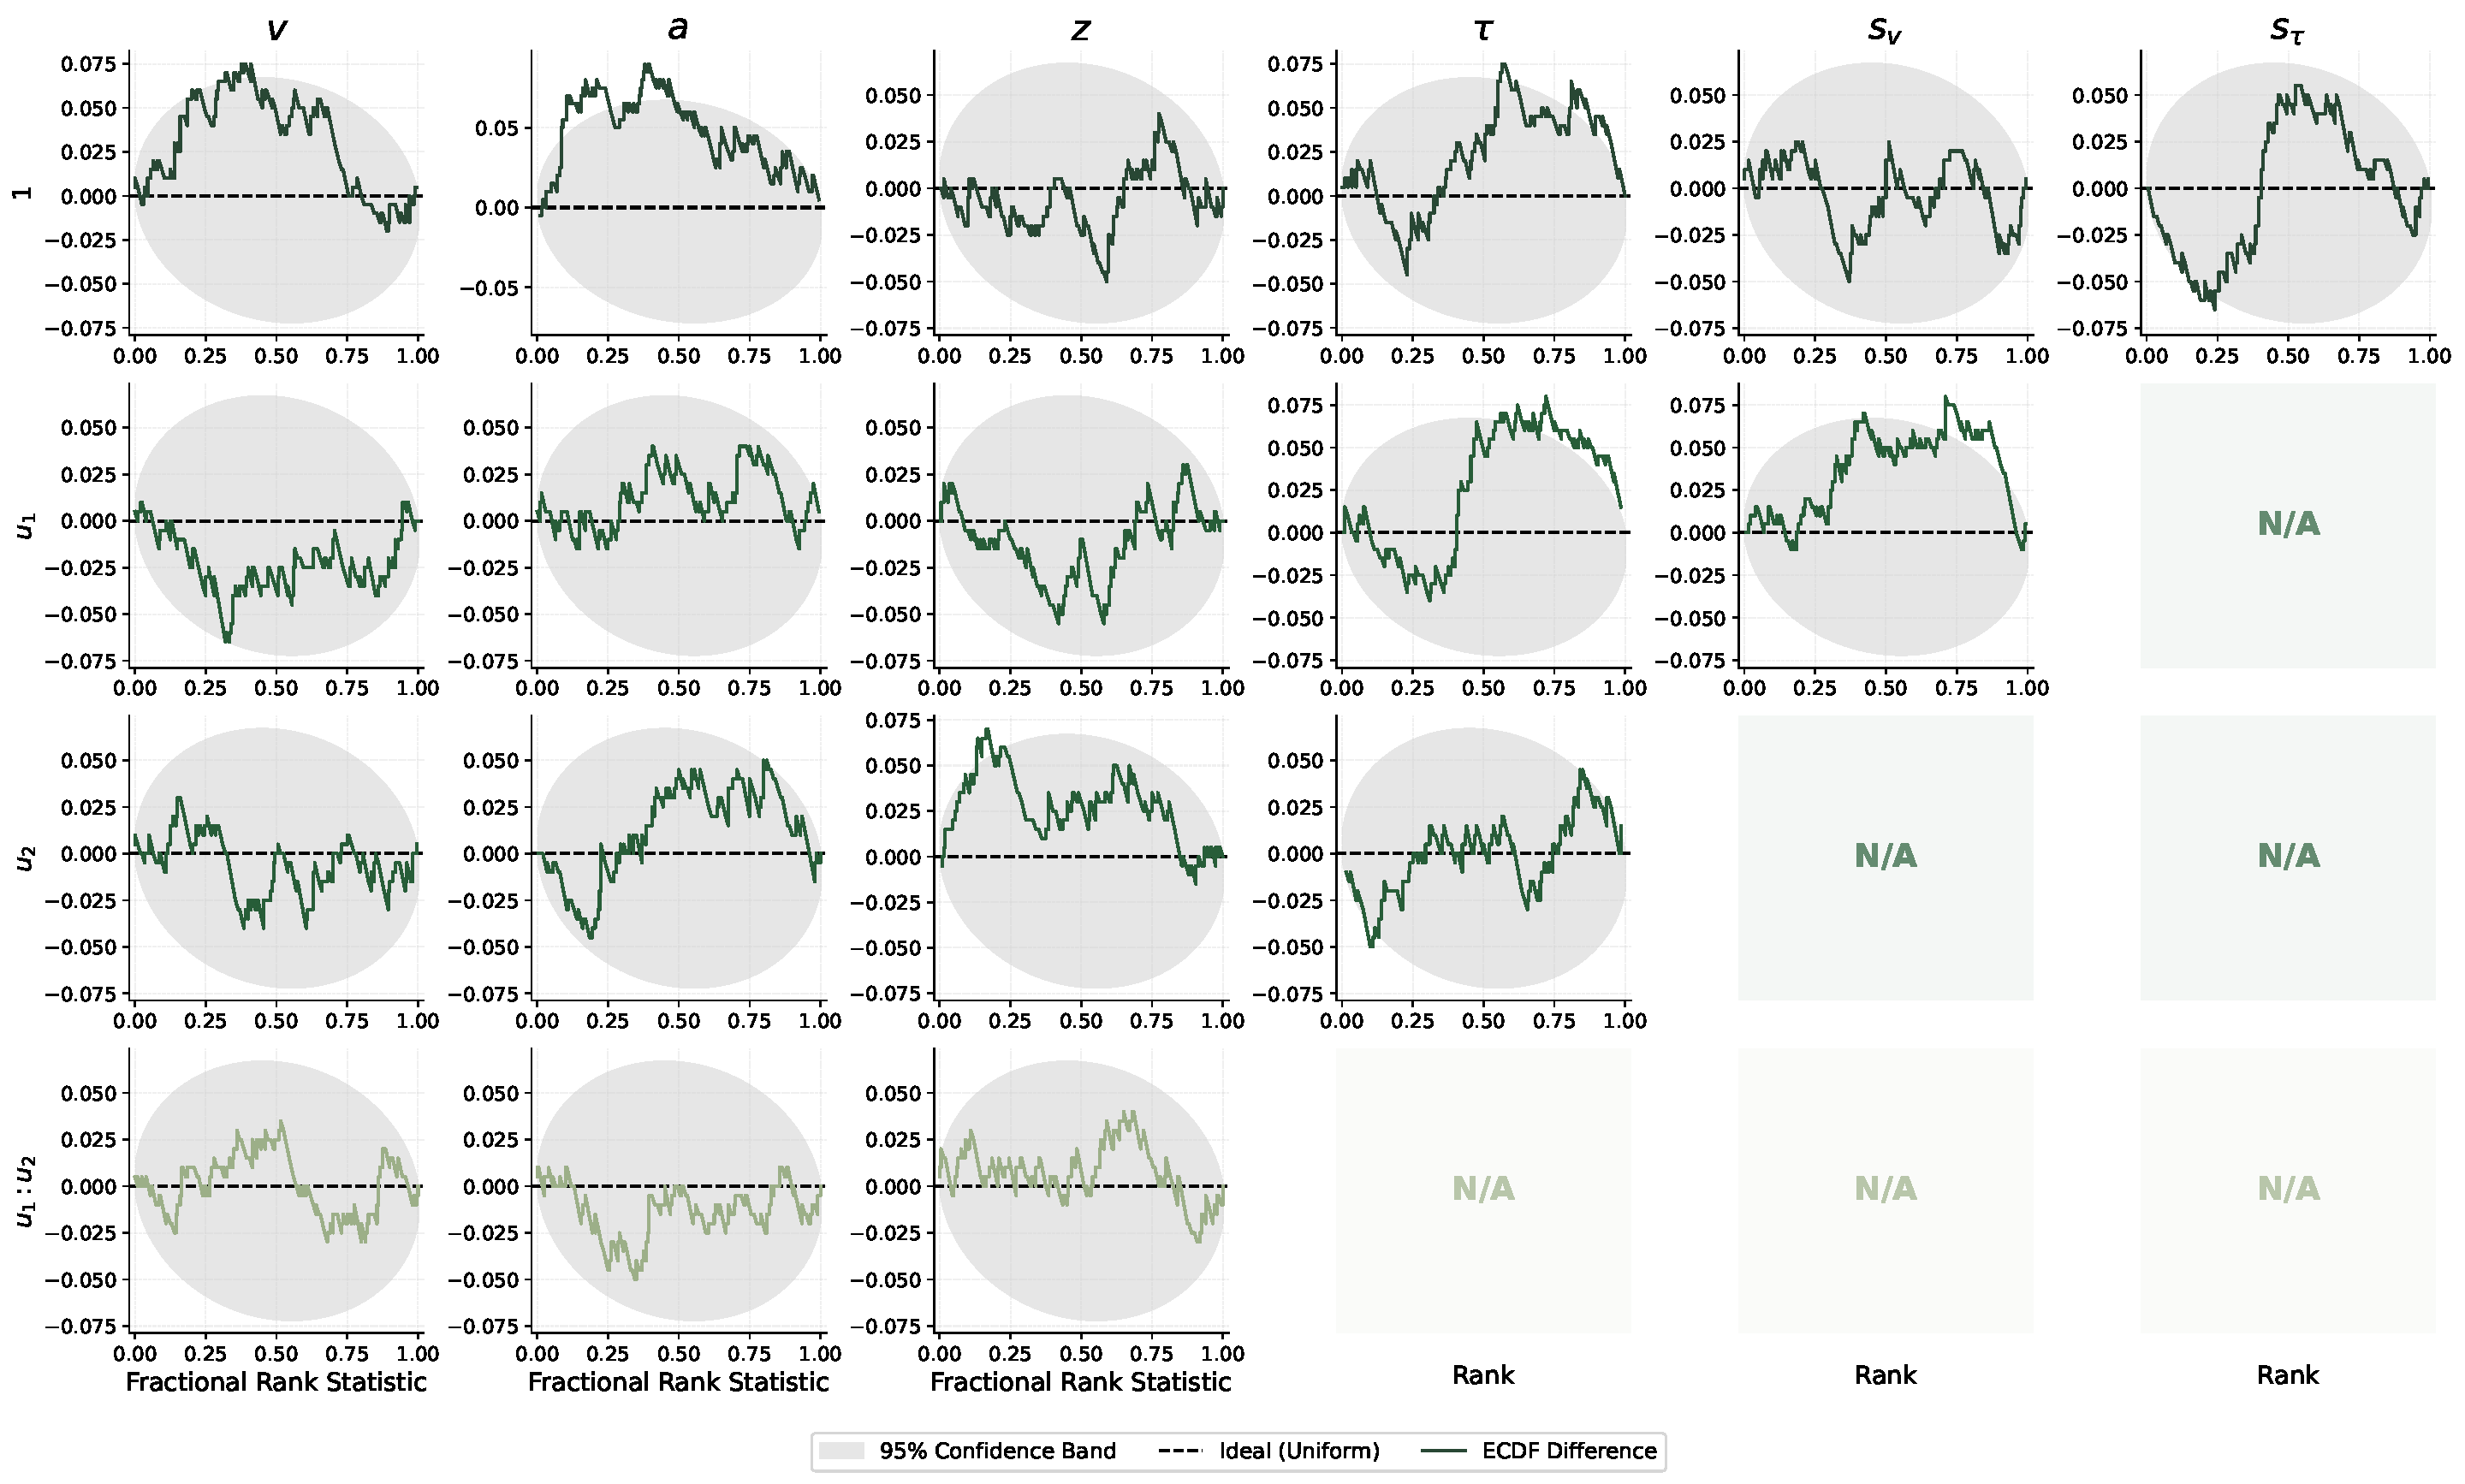
\includegraphics[width=0.99\linewidth]{figures/bf/ddm/interaction/ddm_family_interaction_bf_ecdf.pdf}
    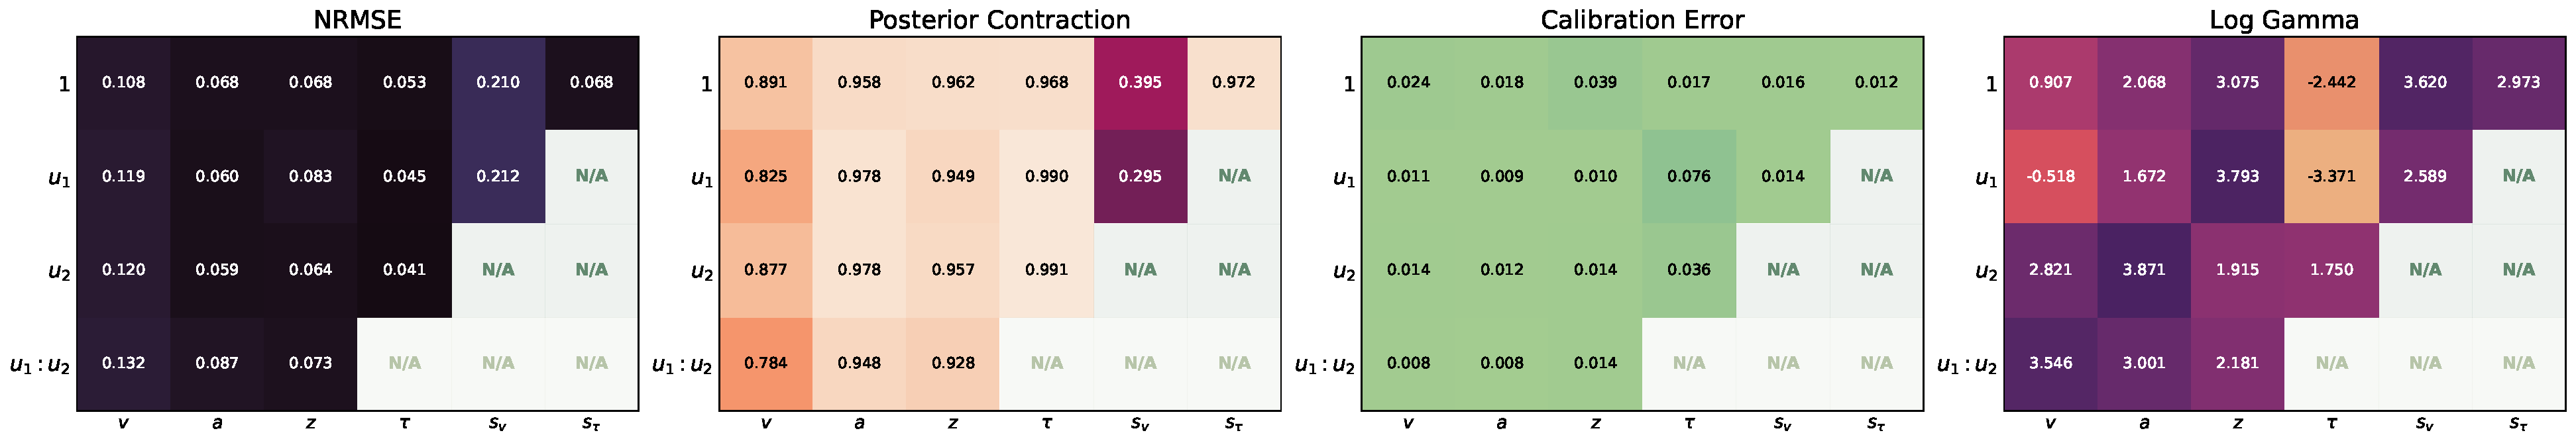
\includegraphics[width=0.99\linewidth]{figures/bf/ddm/interaction/ddm_family_interaction_bf_metrics.pdf}
    \caption{Parameter recovery (\emph{top}), calibration ECDF (\emph{middle}), and parameter-wise metrics (NRMSE, calibration error, and posterior contraction) for DDM baseline (Case \textbf{interaction}).}
    \label{fig:ddm-bf-interaction}
\end{figure}

% ========================================
% DDM MODEL FAMILY (fm)
% ========================================

\begin{figure}
    \centering
    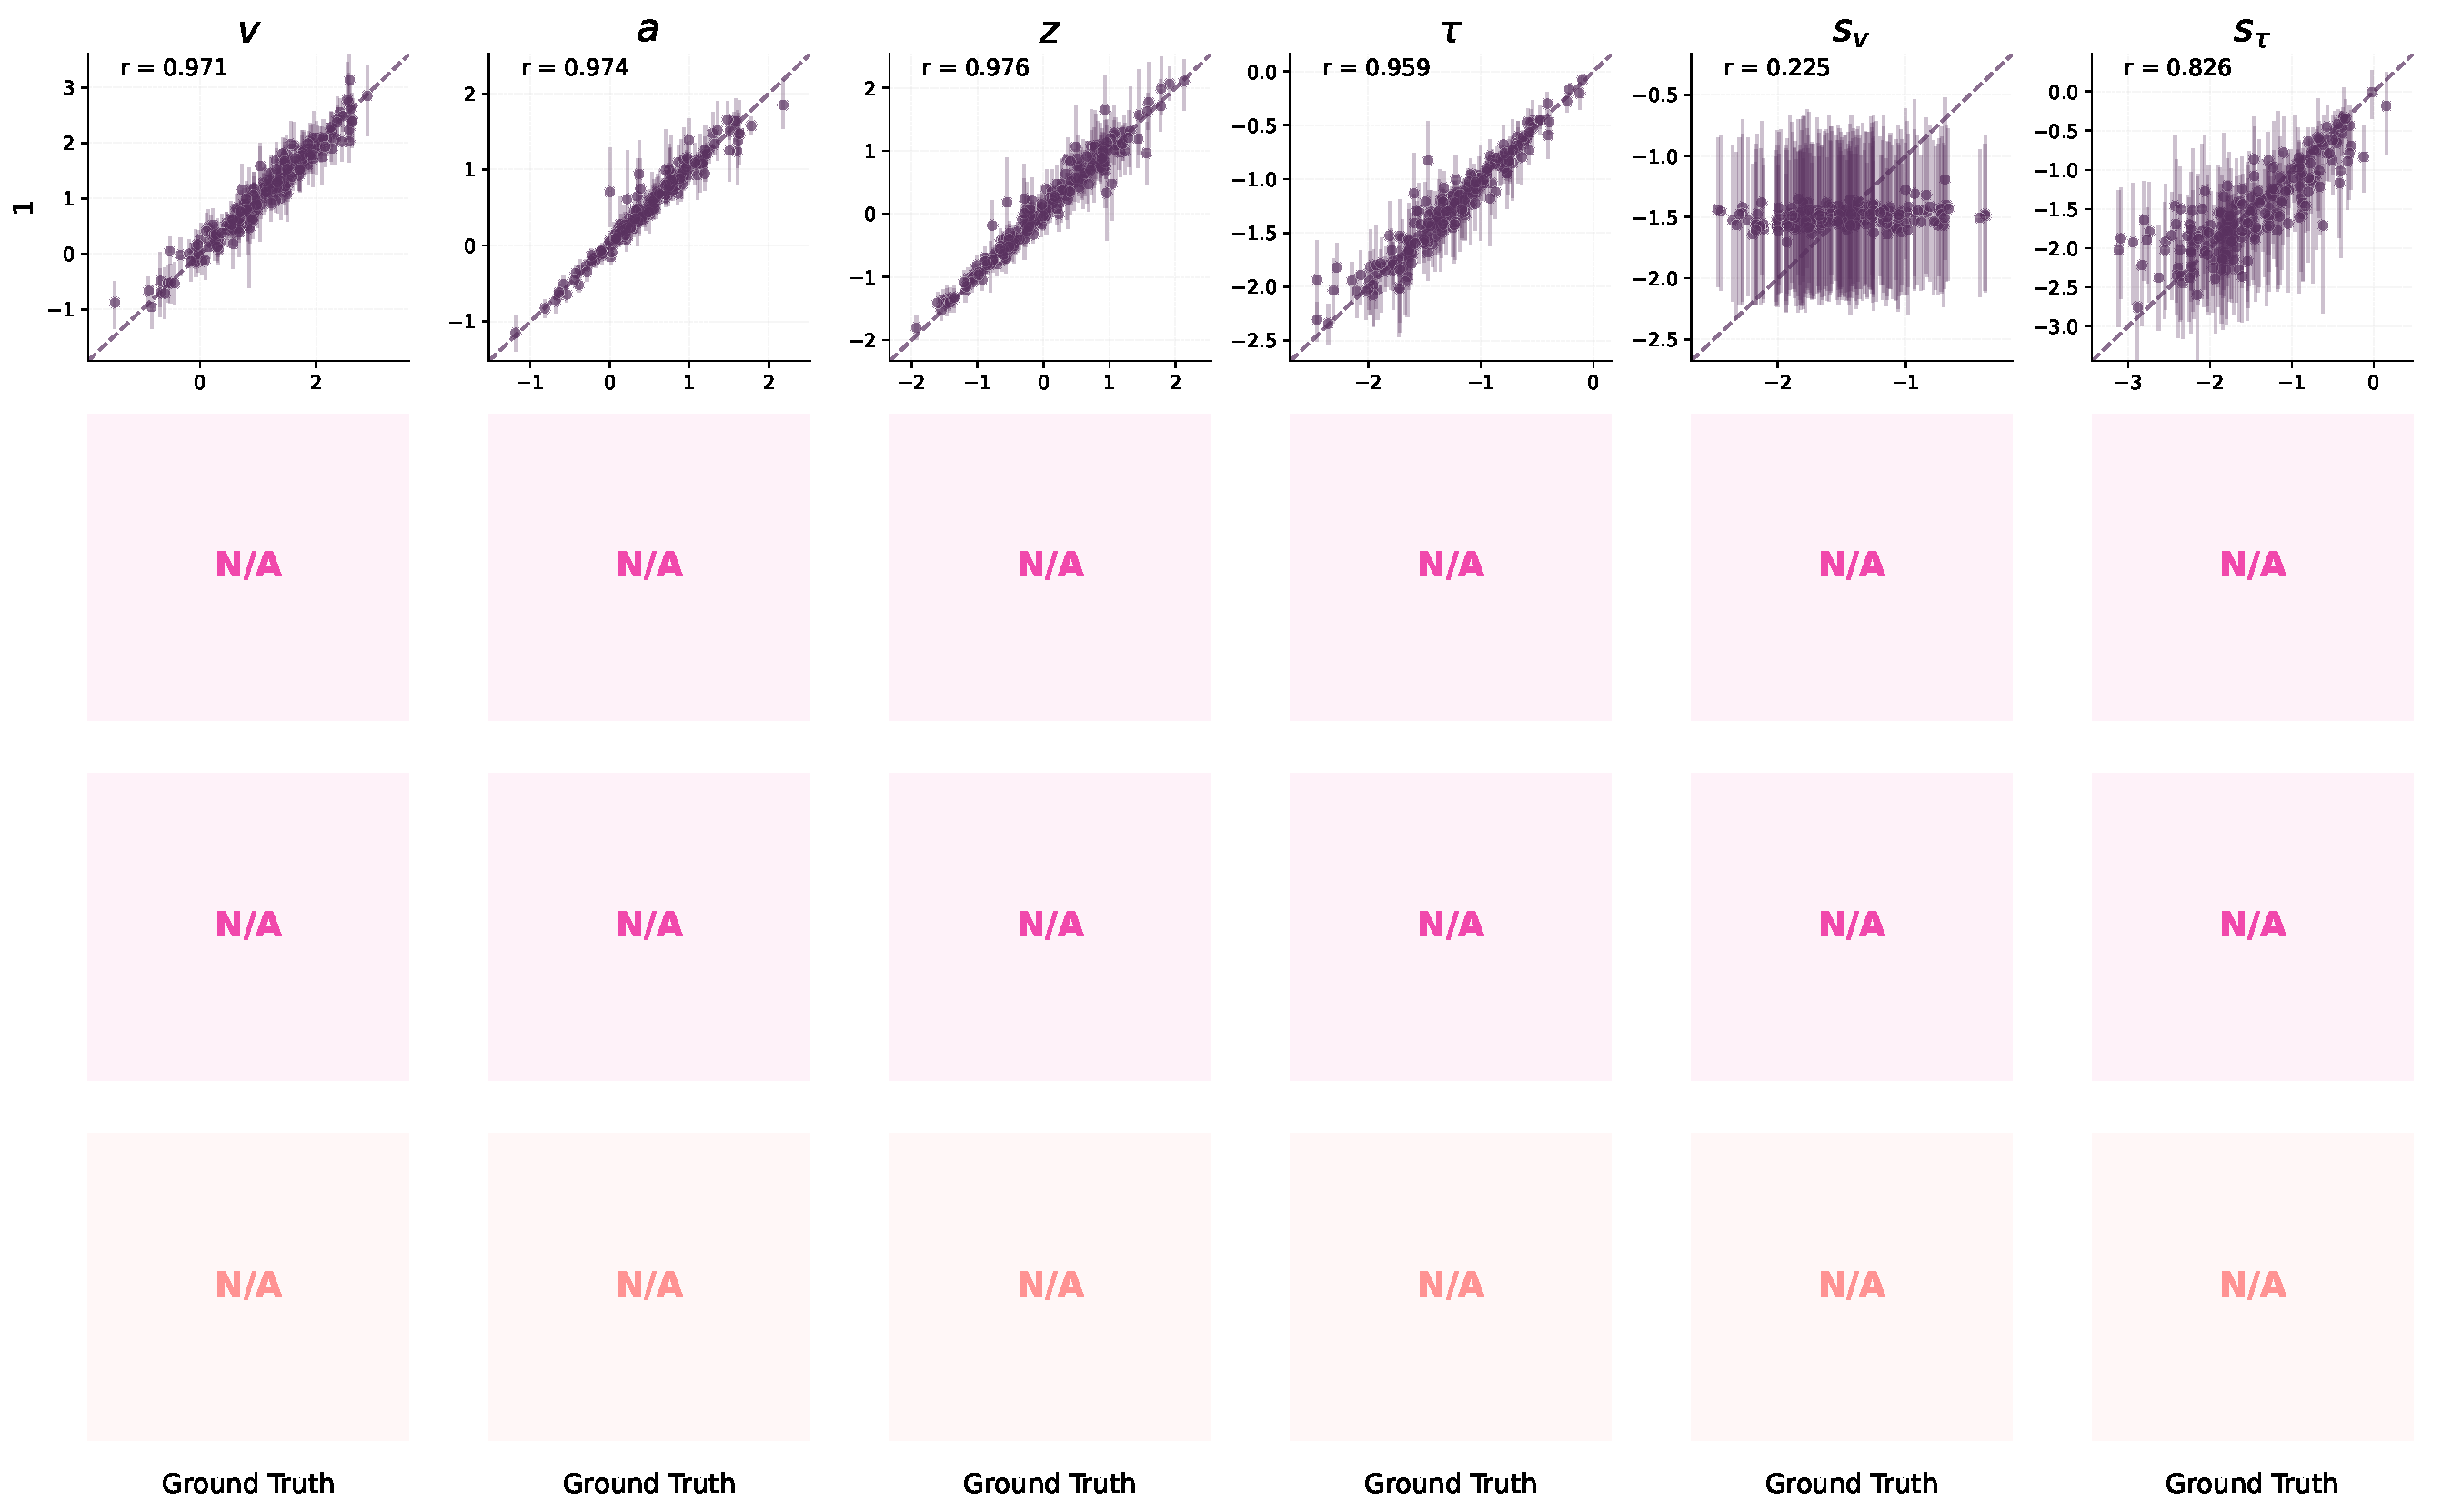
\includegraphics[width=0.99\linewidth]{figures/fm/ddm/intercept_only/ddm_family_intercept_only_fm_mixed_recovery.pdf}
    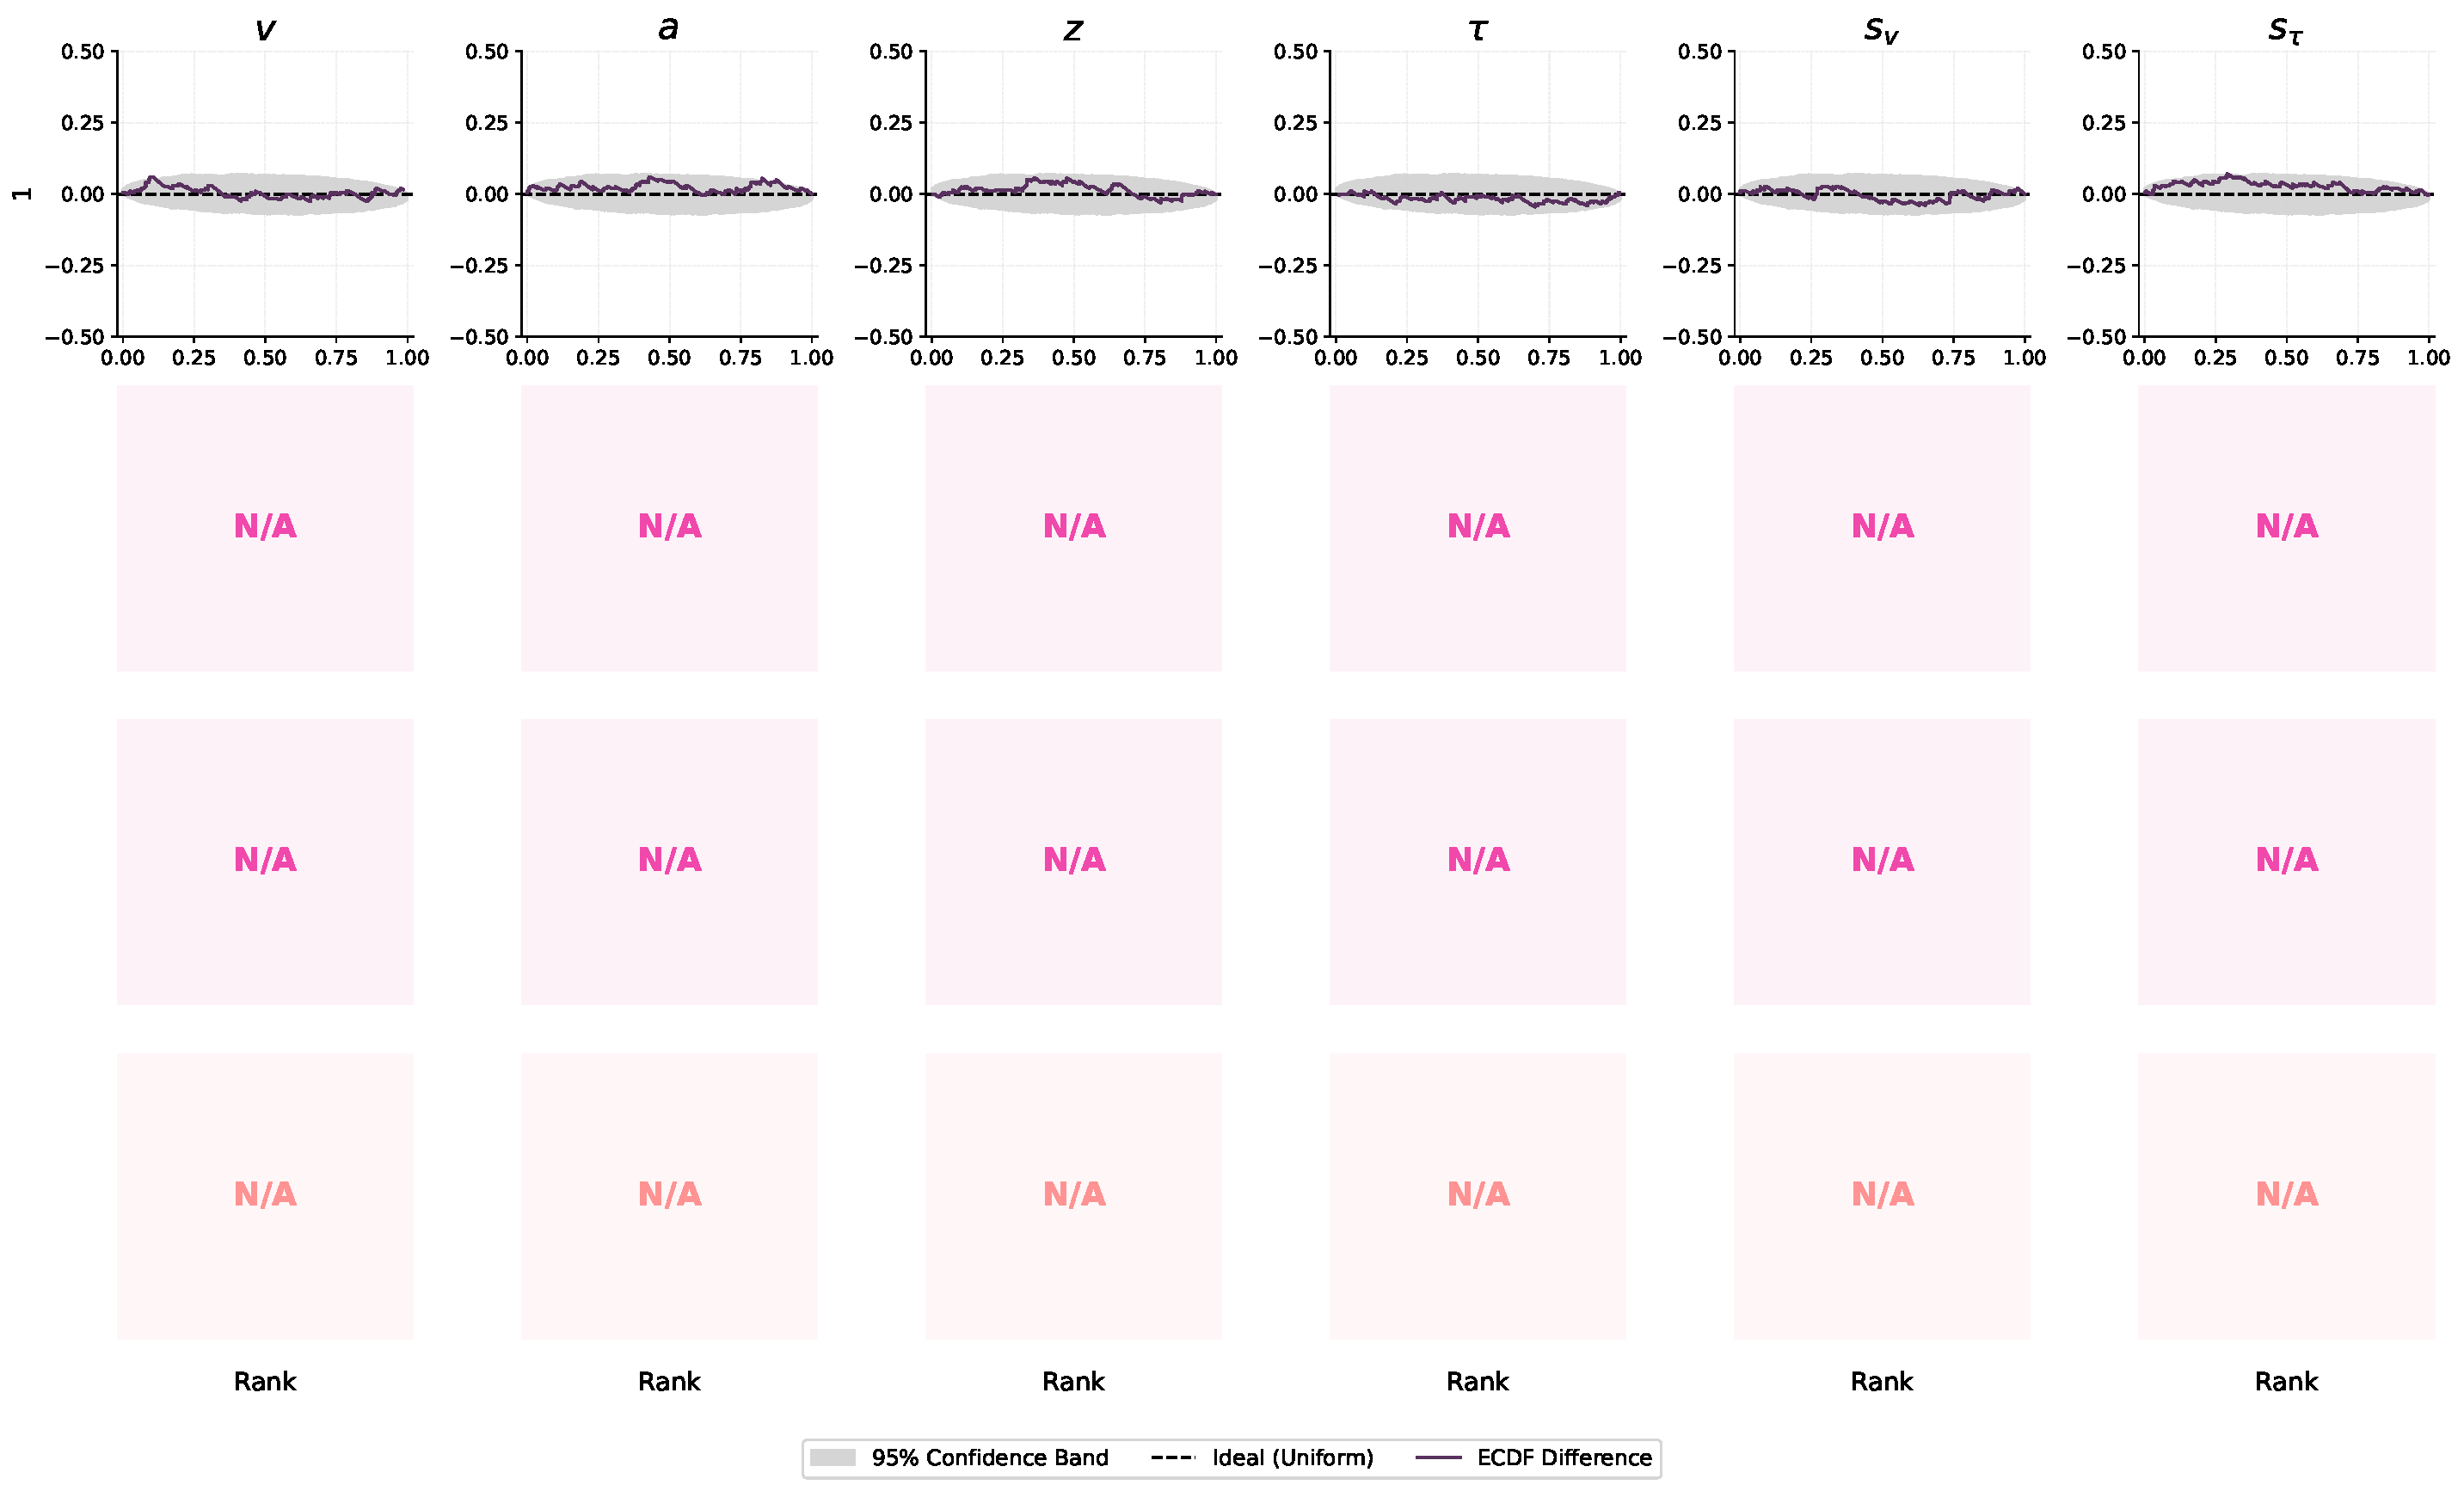
\includegraphics[width=0.99\linewidth]{figures/fm/ddm/intercept_only/ddm_family_intercept_only_fm_mixed_ecdf.pdf}
    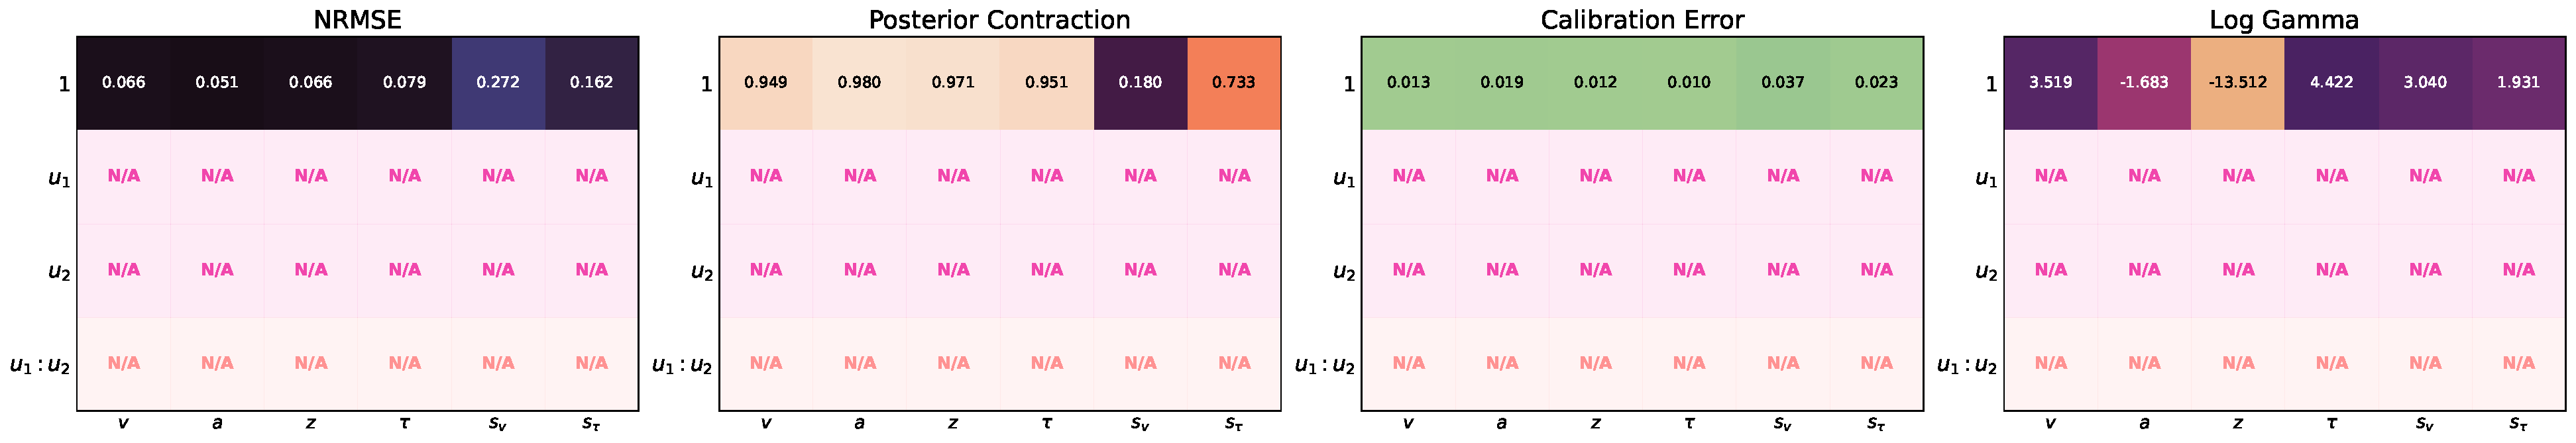
\includegraphics[width=0.99\linewidth]{figures/fm/ddm/intercept_only/ddm_family_intercept_only_fm_mixed_metrics.pdf}
    \caption{Parameter recovery (\emph{top}), calibration ECDF (\emph{middle}), and parameter-wise metrics (NRMSE, calibration error, and posterior contraction) for DDM model family (Case \textbf{intercept\_only}).}
    \label{fig:ddm-fm-intercept-only}
\end{figure}

\begin{figure}
    \centering
    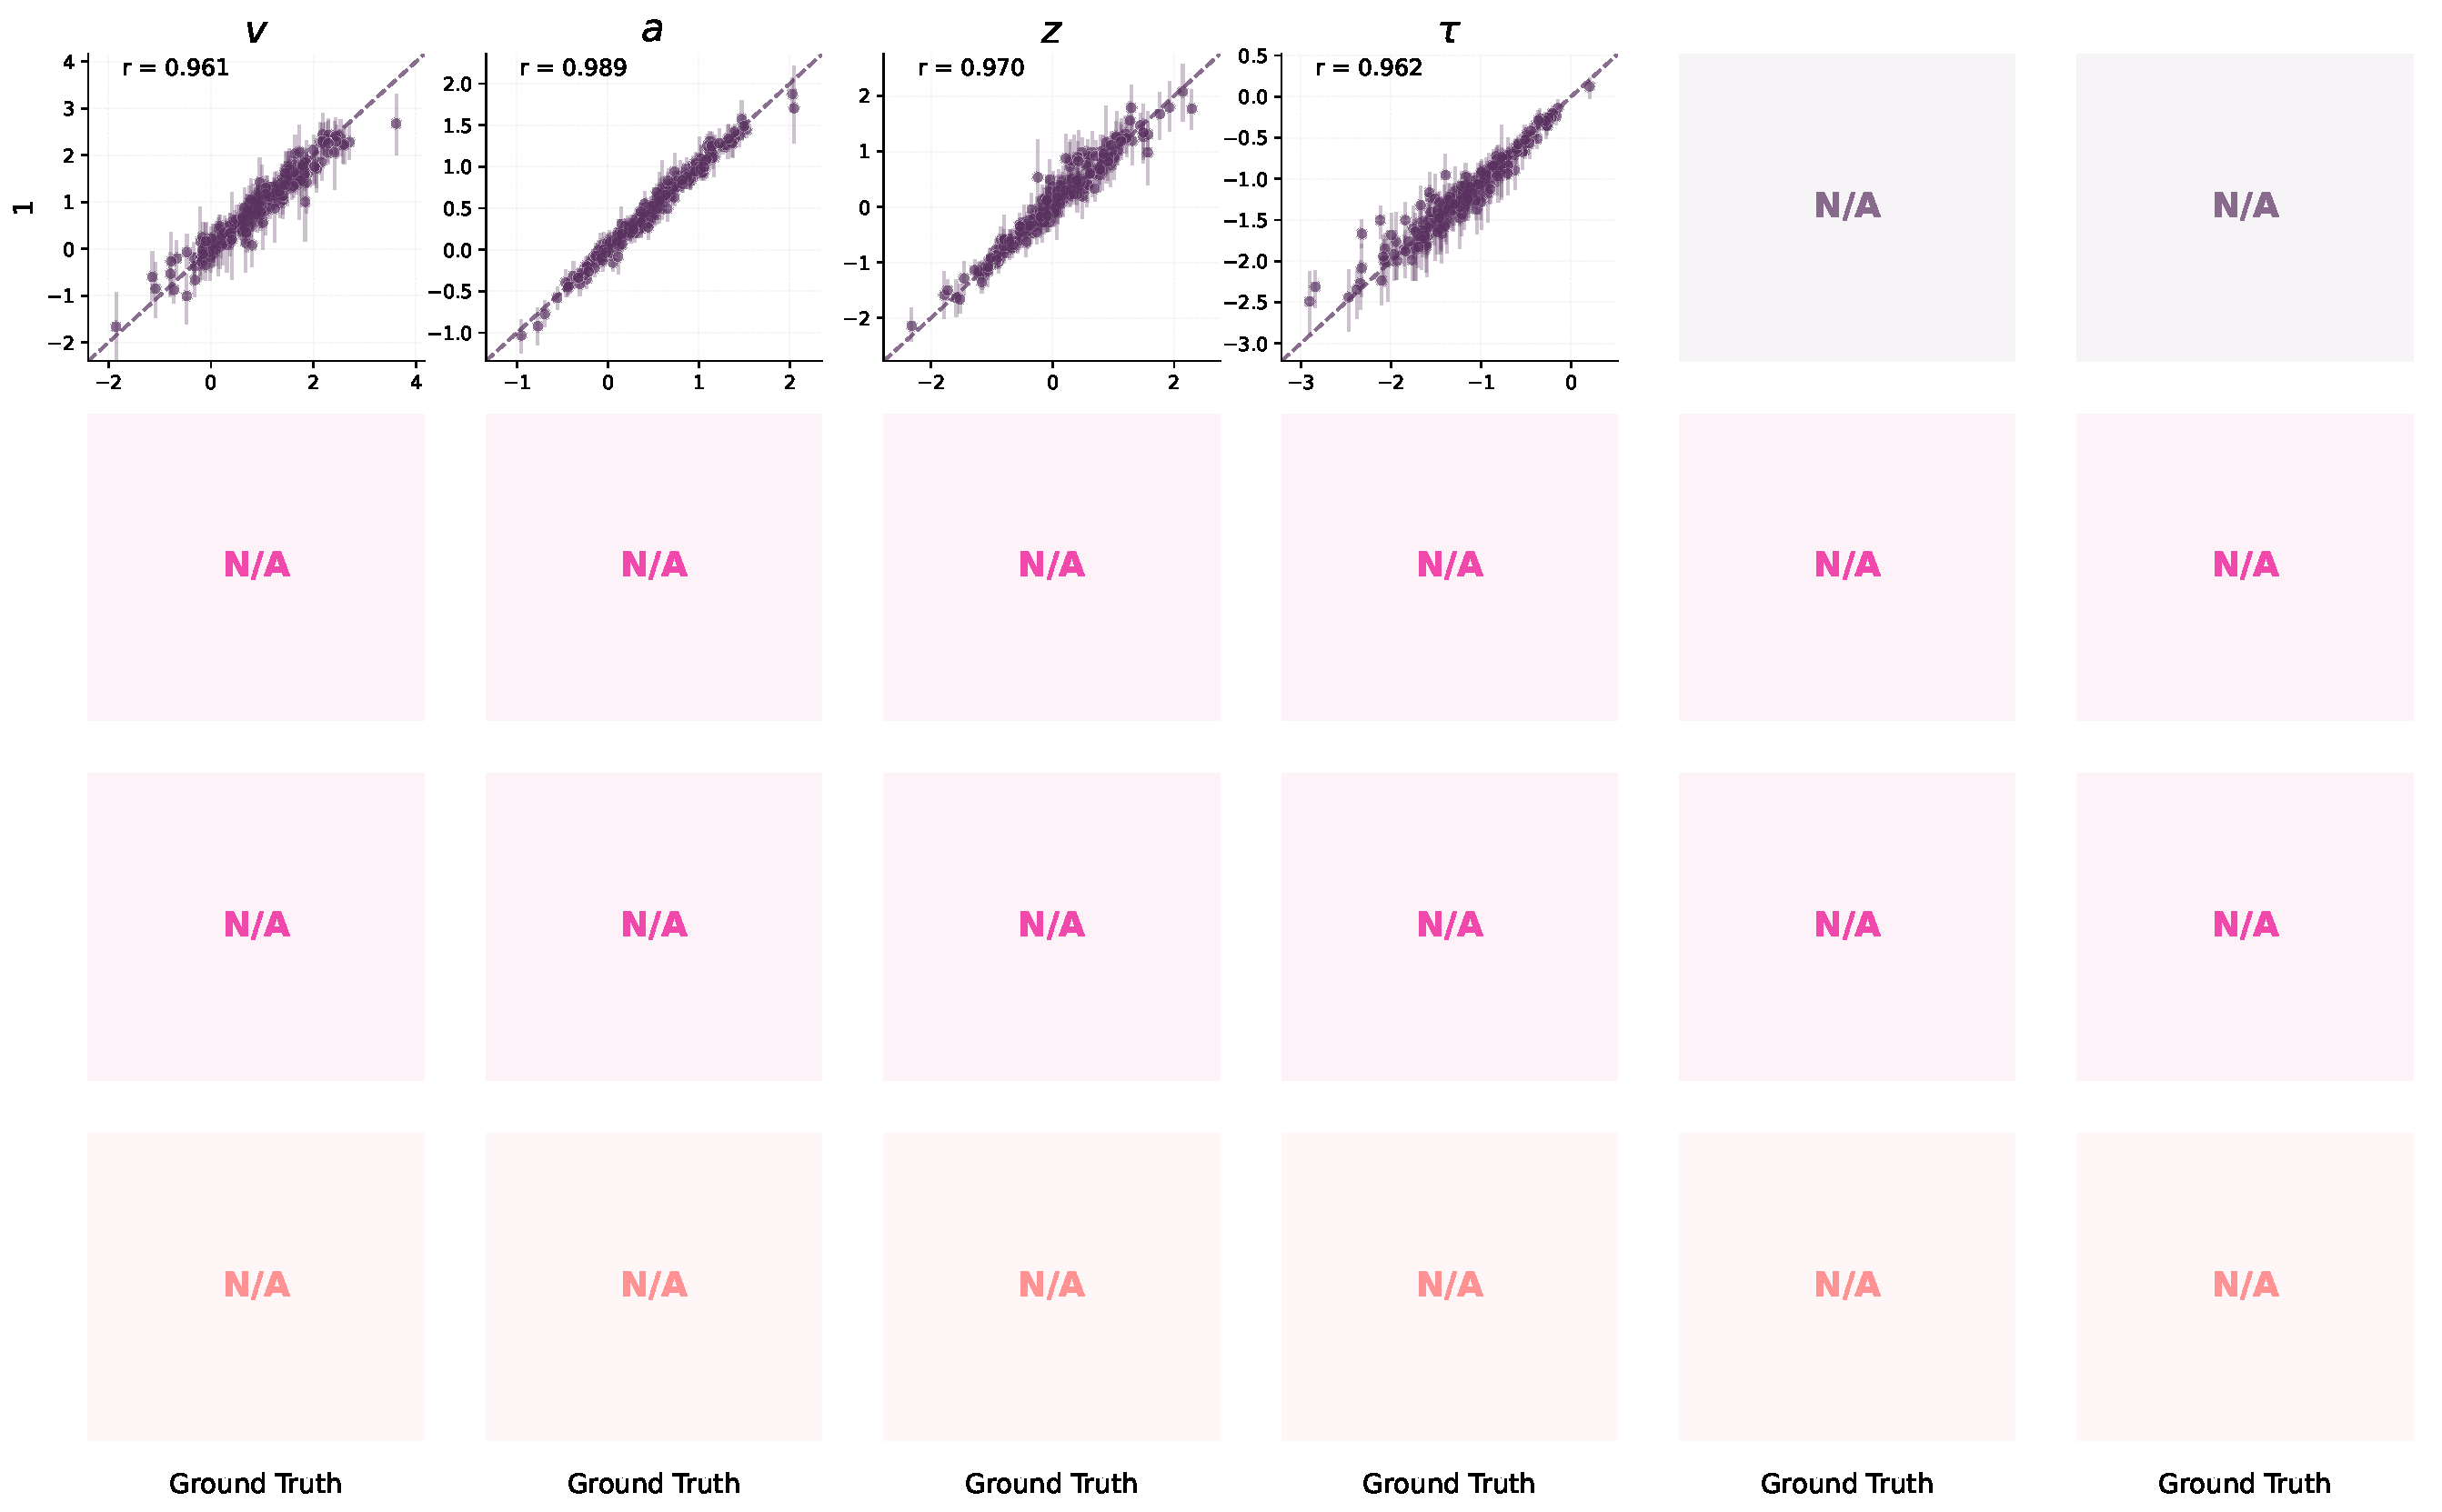
\includegraphics[width=0.99\linewidth]{figures/fm/ddm/fixed/ddm_family_fixed_fm_mixed_recovery.pdf}
    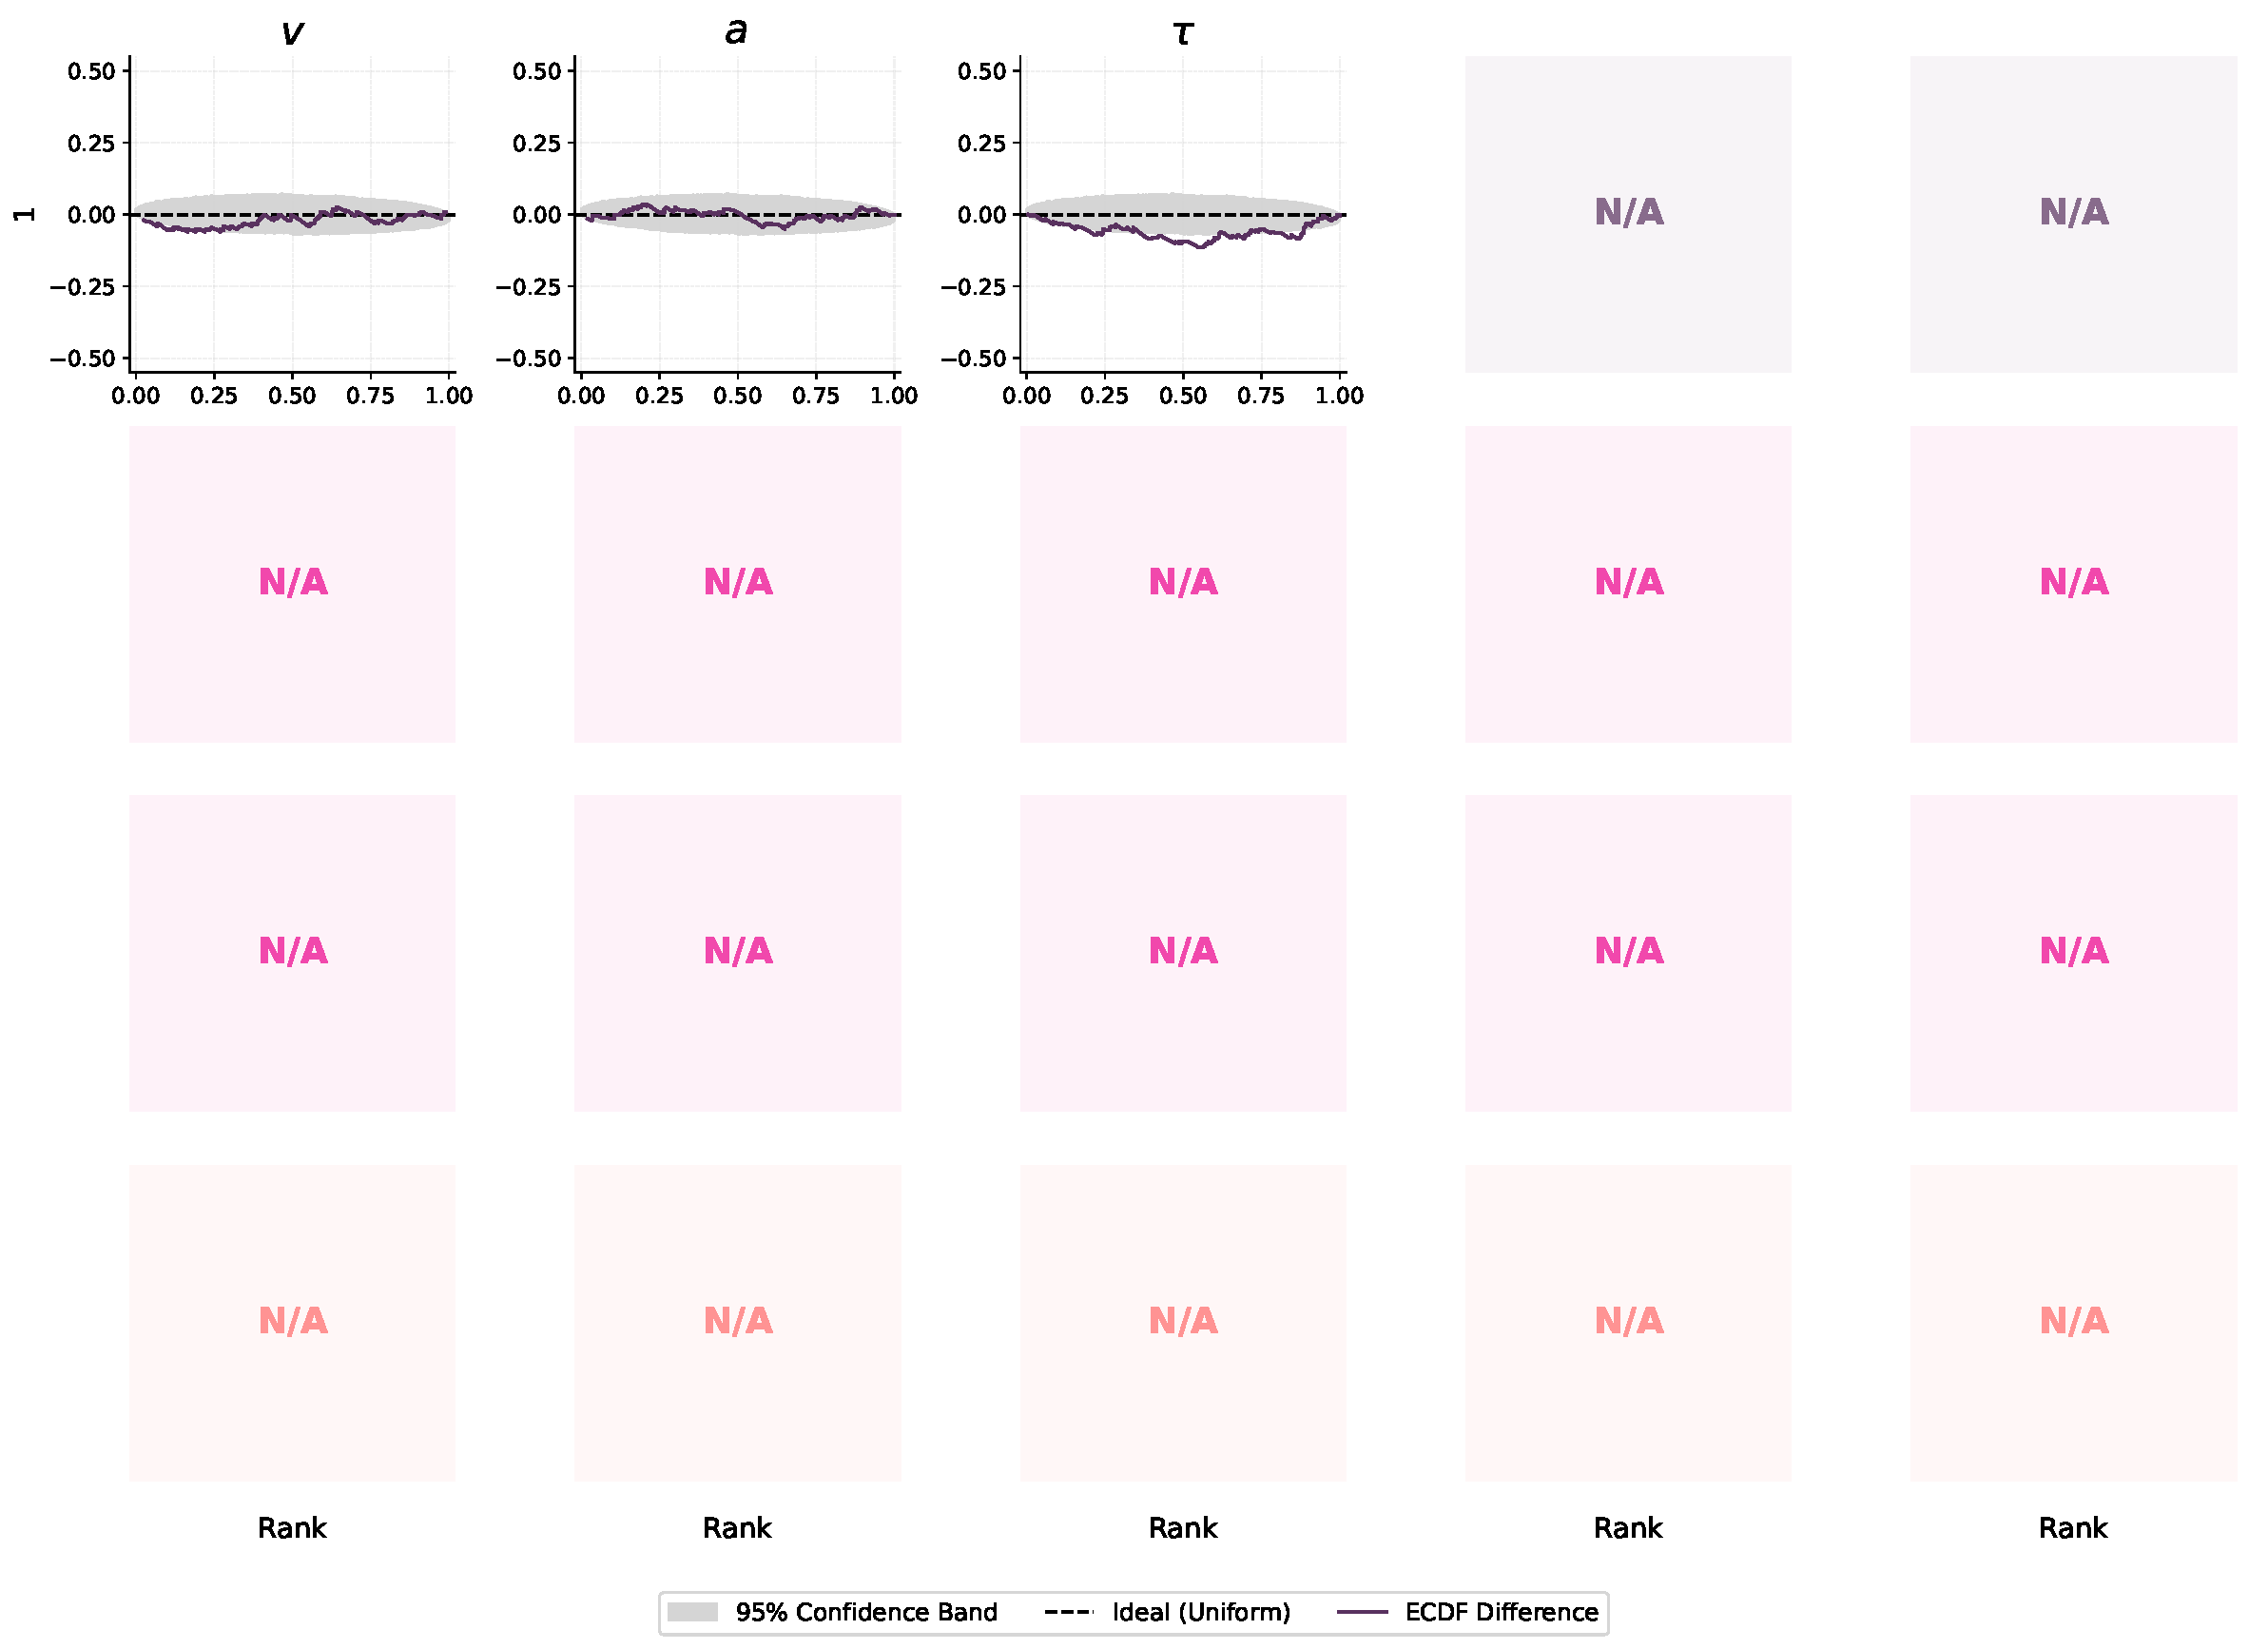
\includegraphics[width=0.99\linewidth]{figures/fm/ddm/fixed/ddm_family_fixed_fm_mixed_ecdf.pdf}
    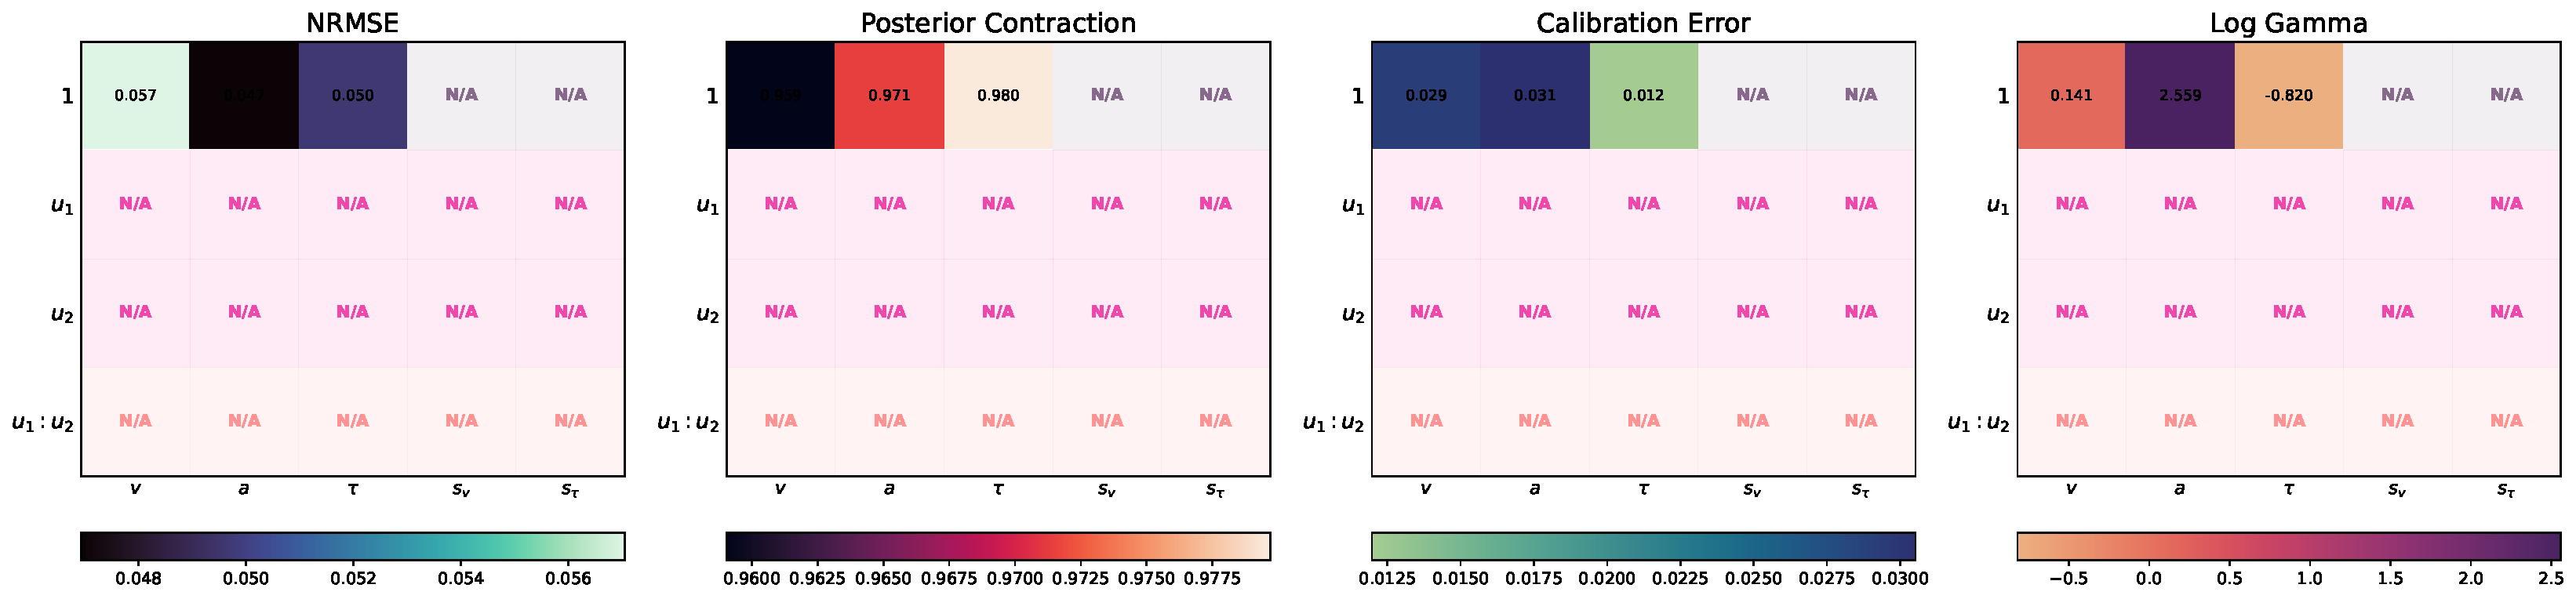
\includegraphics[width=0.99\linewidth]{figures/fm/ddm/fixed/ddm_family_fixed_fm_mixed_metrics.pdf}
    \caption{Parameter recovery (\emph{top}), calibration ECDF (\emph{middle}), and parameter-wise metrics (NRMSE, calibration error, and posterior contraction) for DDM model family (Case \textbf{fixed}).}
    \label{fig:ddm-fm-fixed}
\end{figure}

\begin{figure}
    \centering
    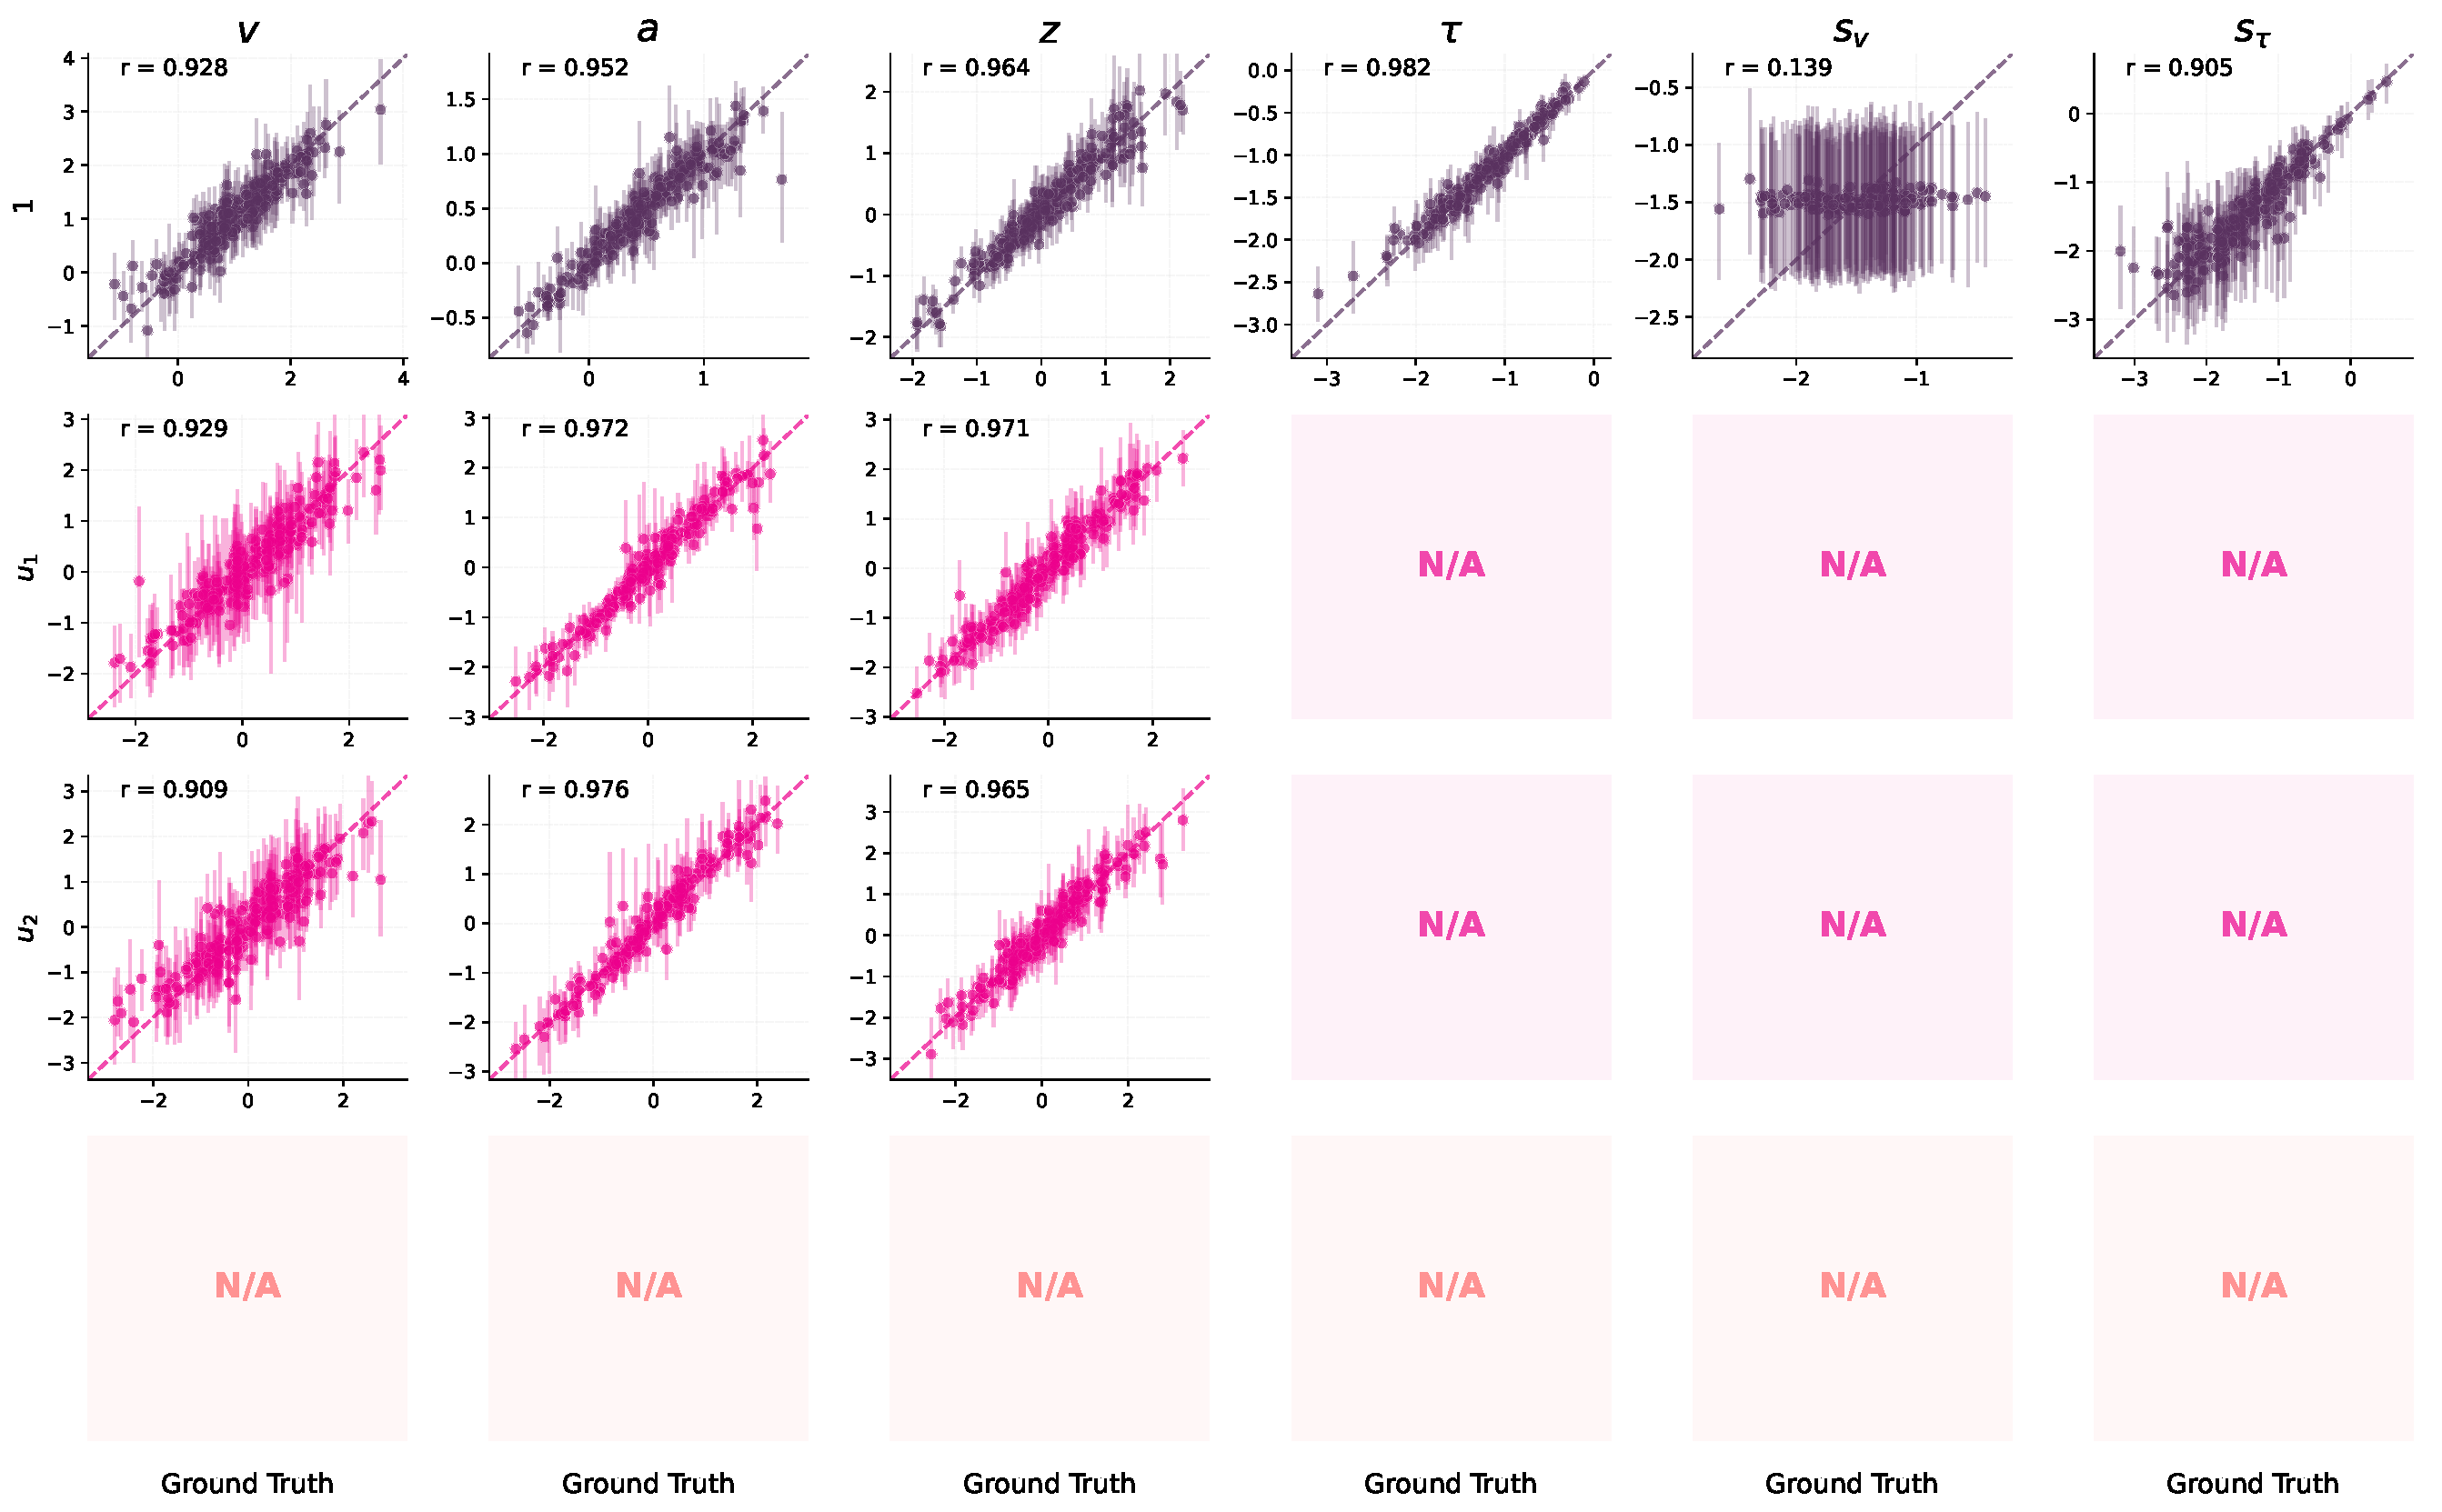
\includegraphics[width=0.99\linewidth]{figures/fm/ddm/regressed/ddm_family_regressed_fm_mixed_recovery.pdf}
    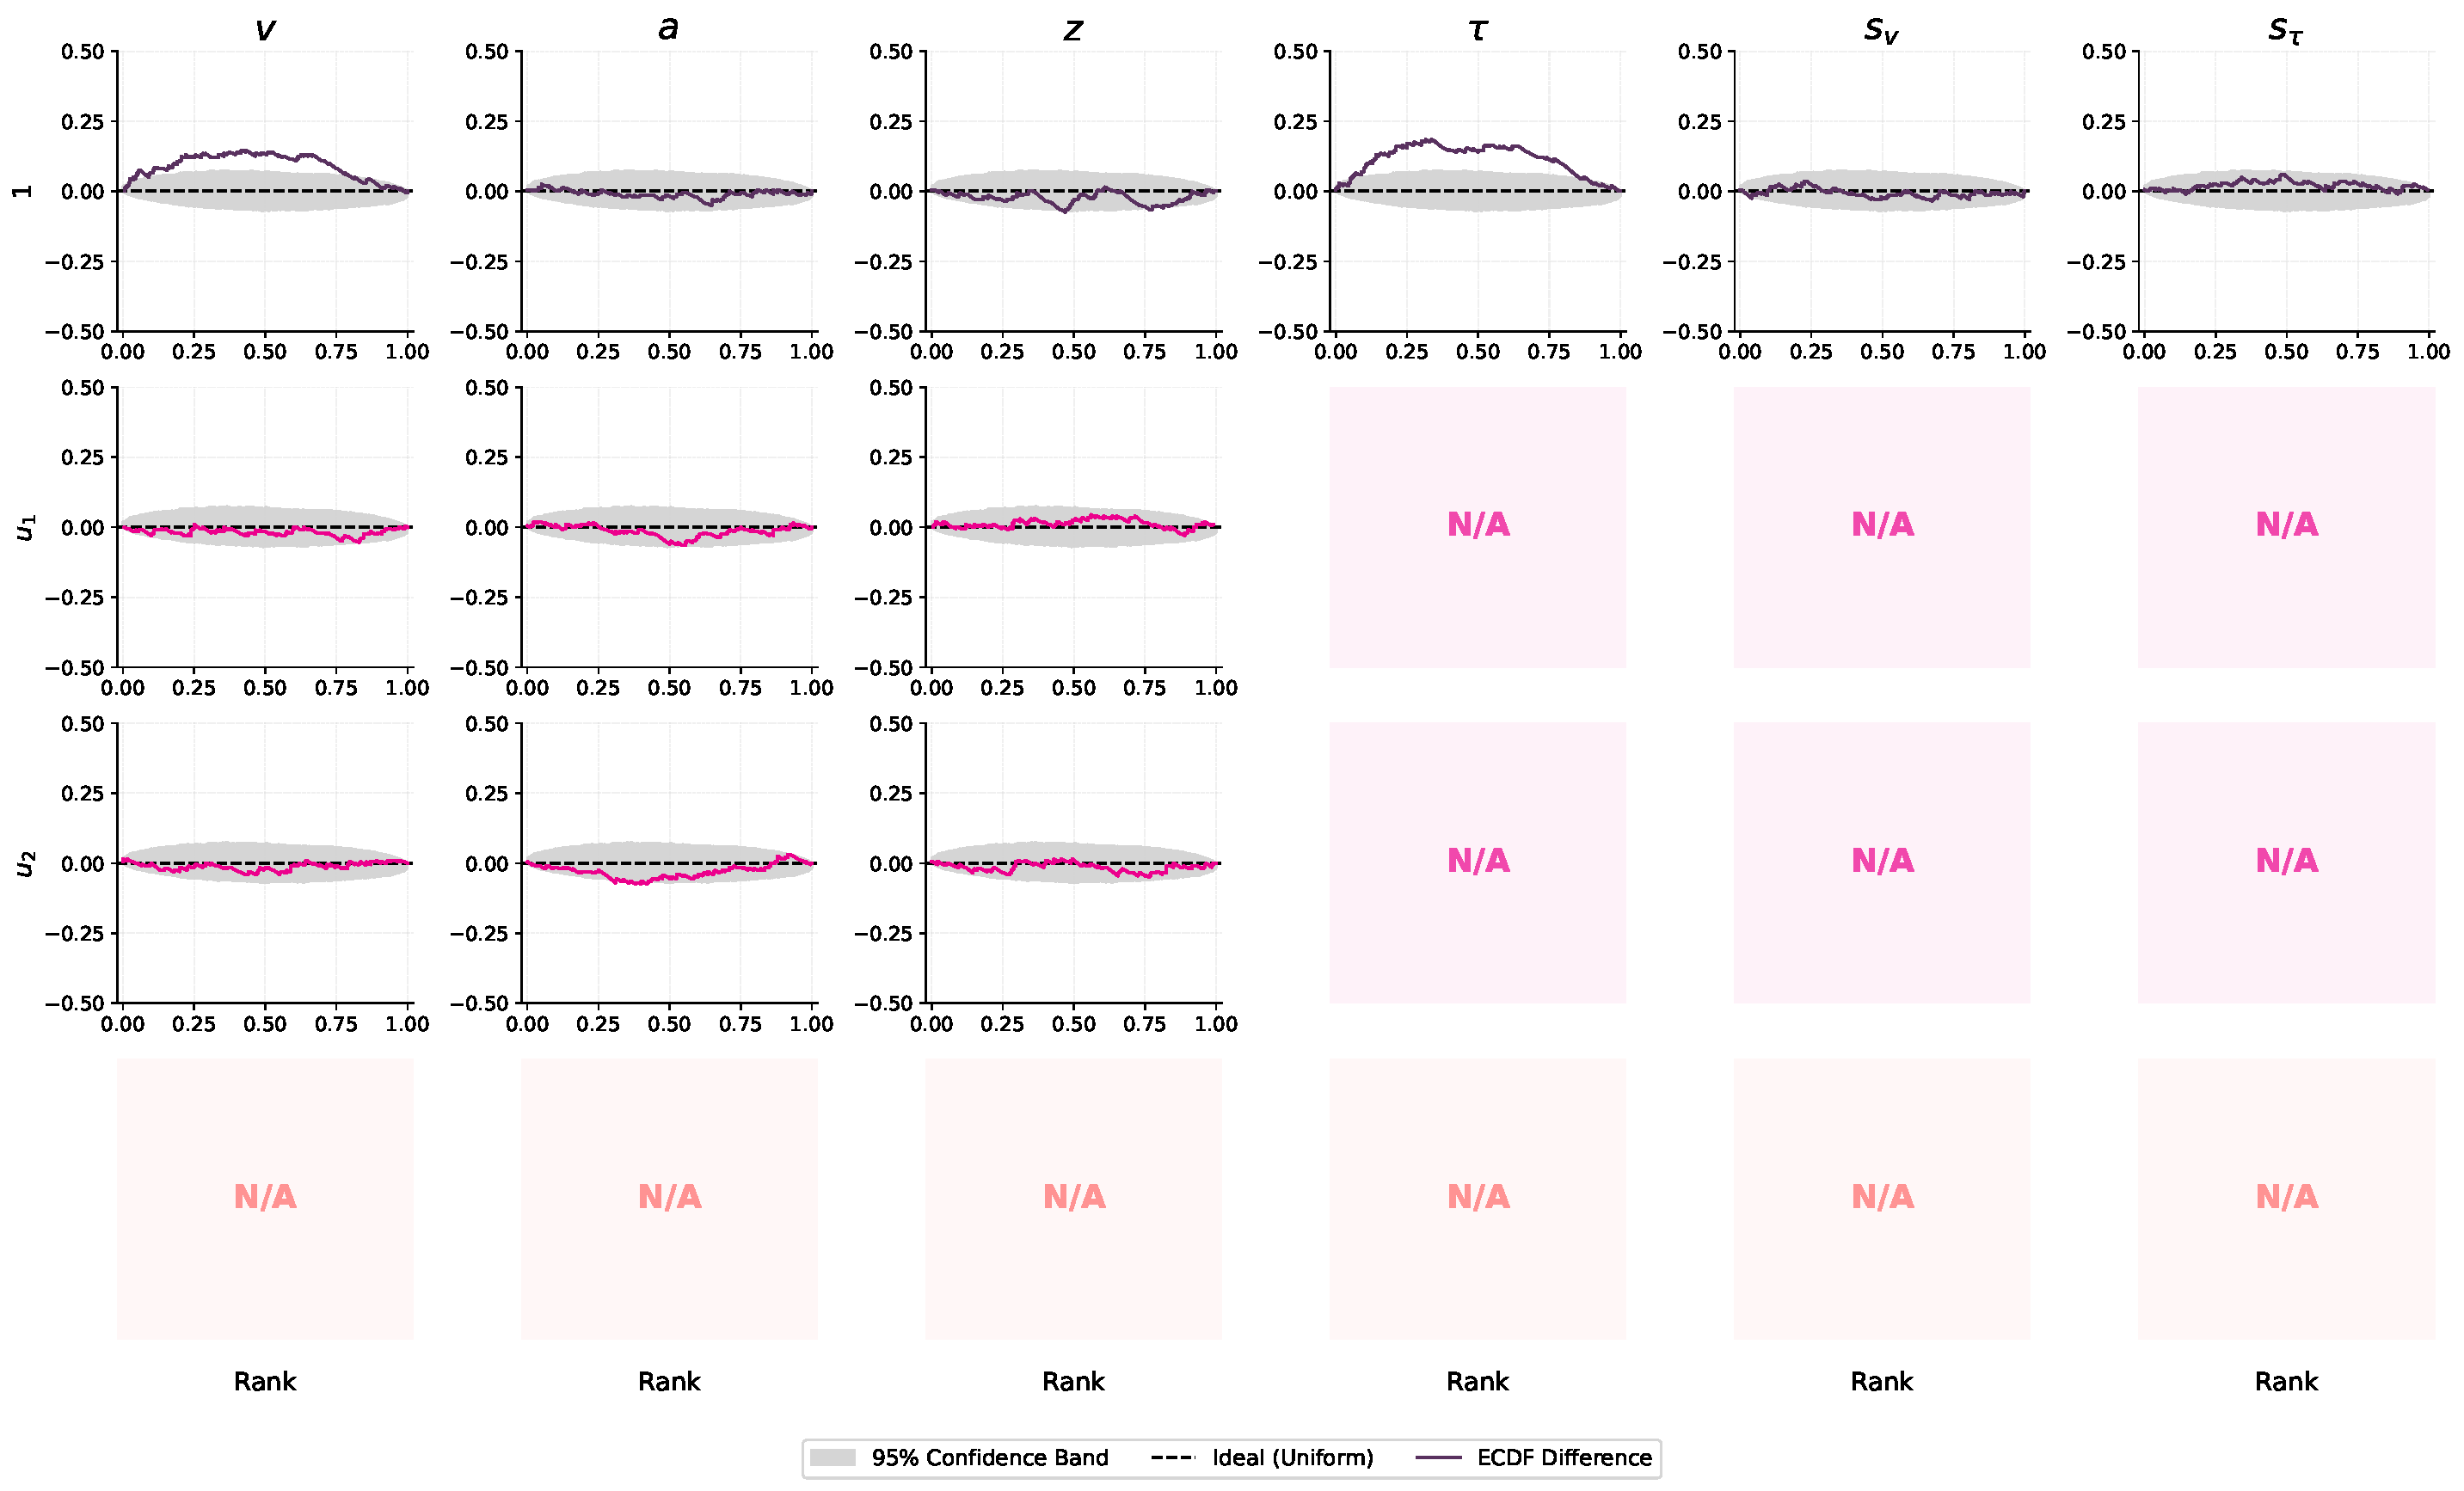
\includegraphics[width=0.99\linewidth]{figures/fm/ddm/regressed/ddm_family_regressed_fm_mixed_ecdf.pdf}
    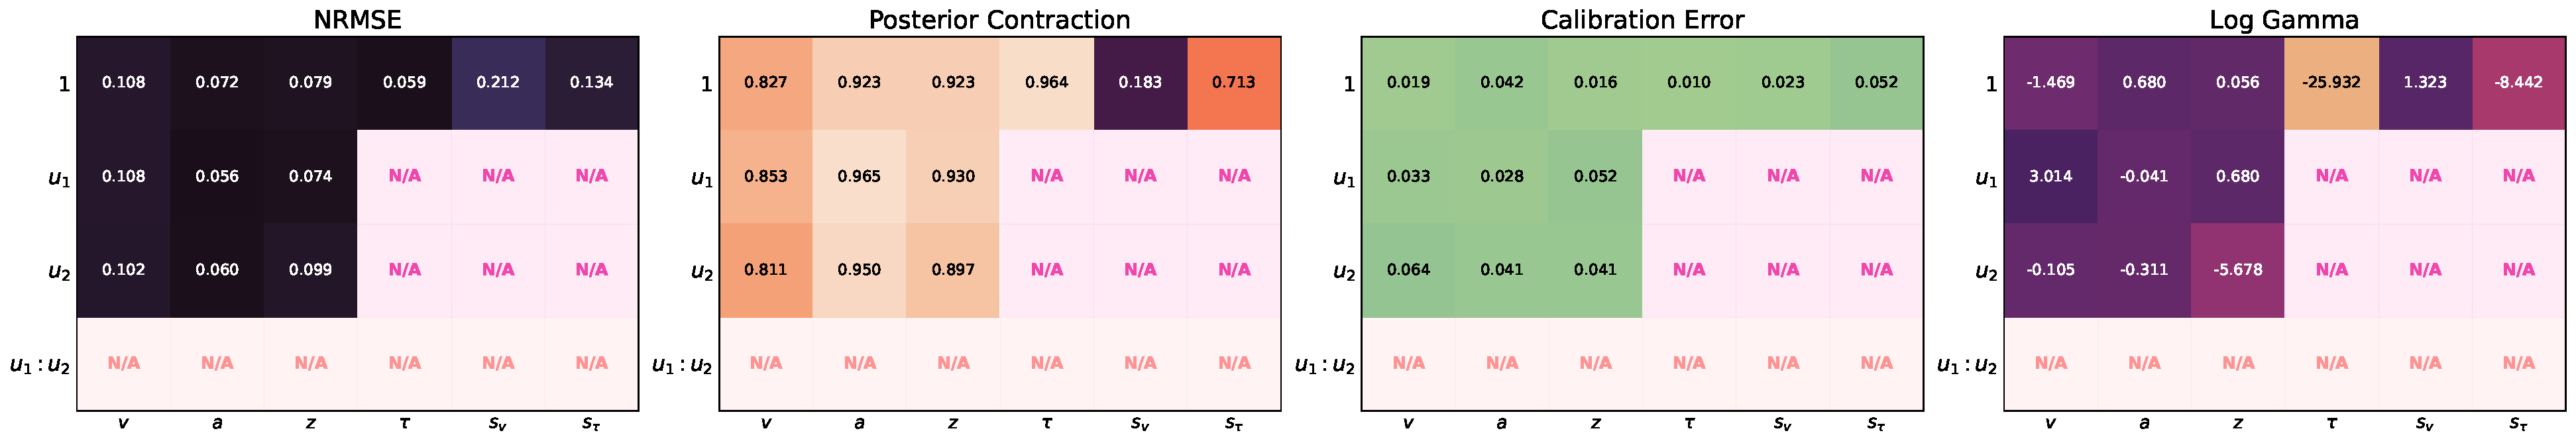
\includegraphics[width=0.99\linewidth]{figures/fm/ddm/regressed/ddm_family_regressed_fm_mixed_metrics.pdf}
    \caption{Parameter recovery (\emph{top}), calibration ECDF (\emph{middle}), and parameter-wise metrics (NRMSE, calibration error, and posterior contraction) for DDM model family (Case \textbf{regressed}).}
    \label{fig:ddm-fm-regressed}
\end{figure}

\begin{figure}
    \centering
    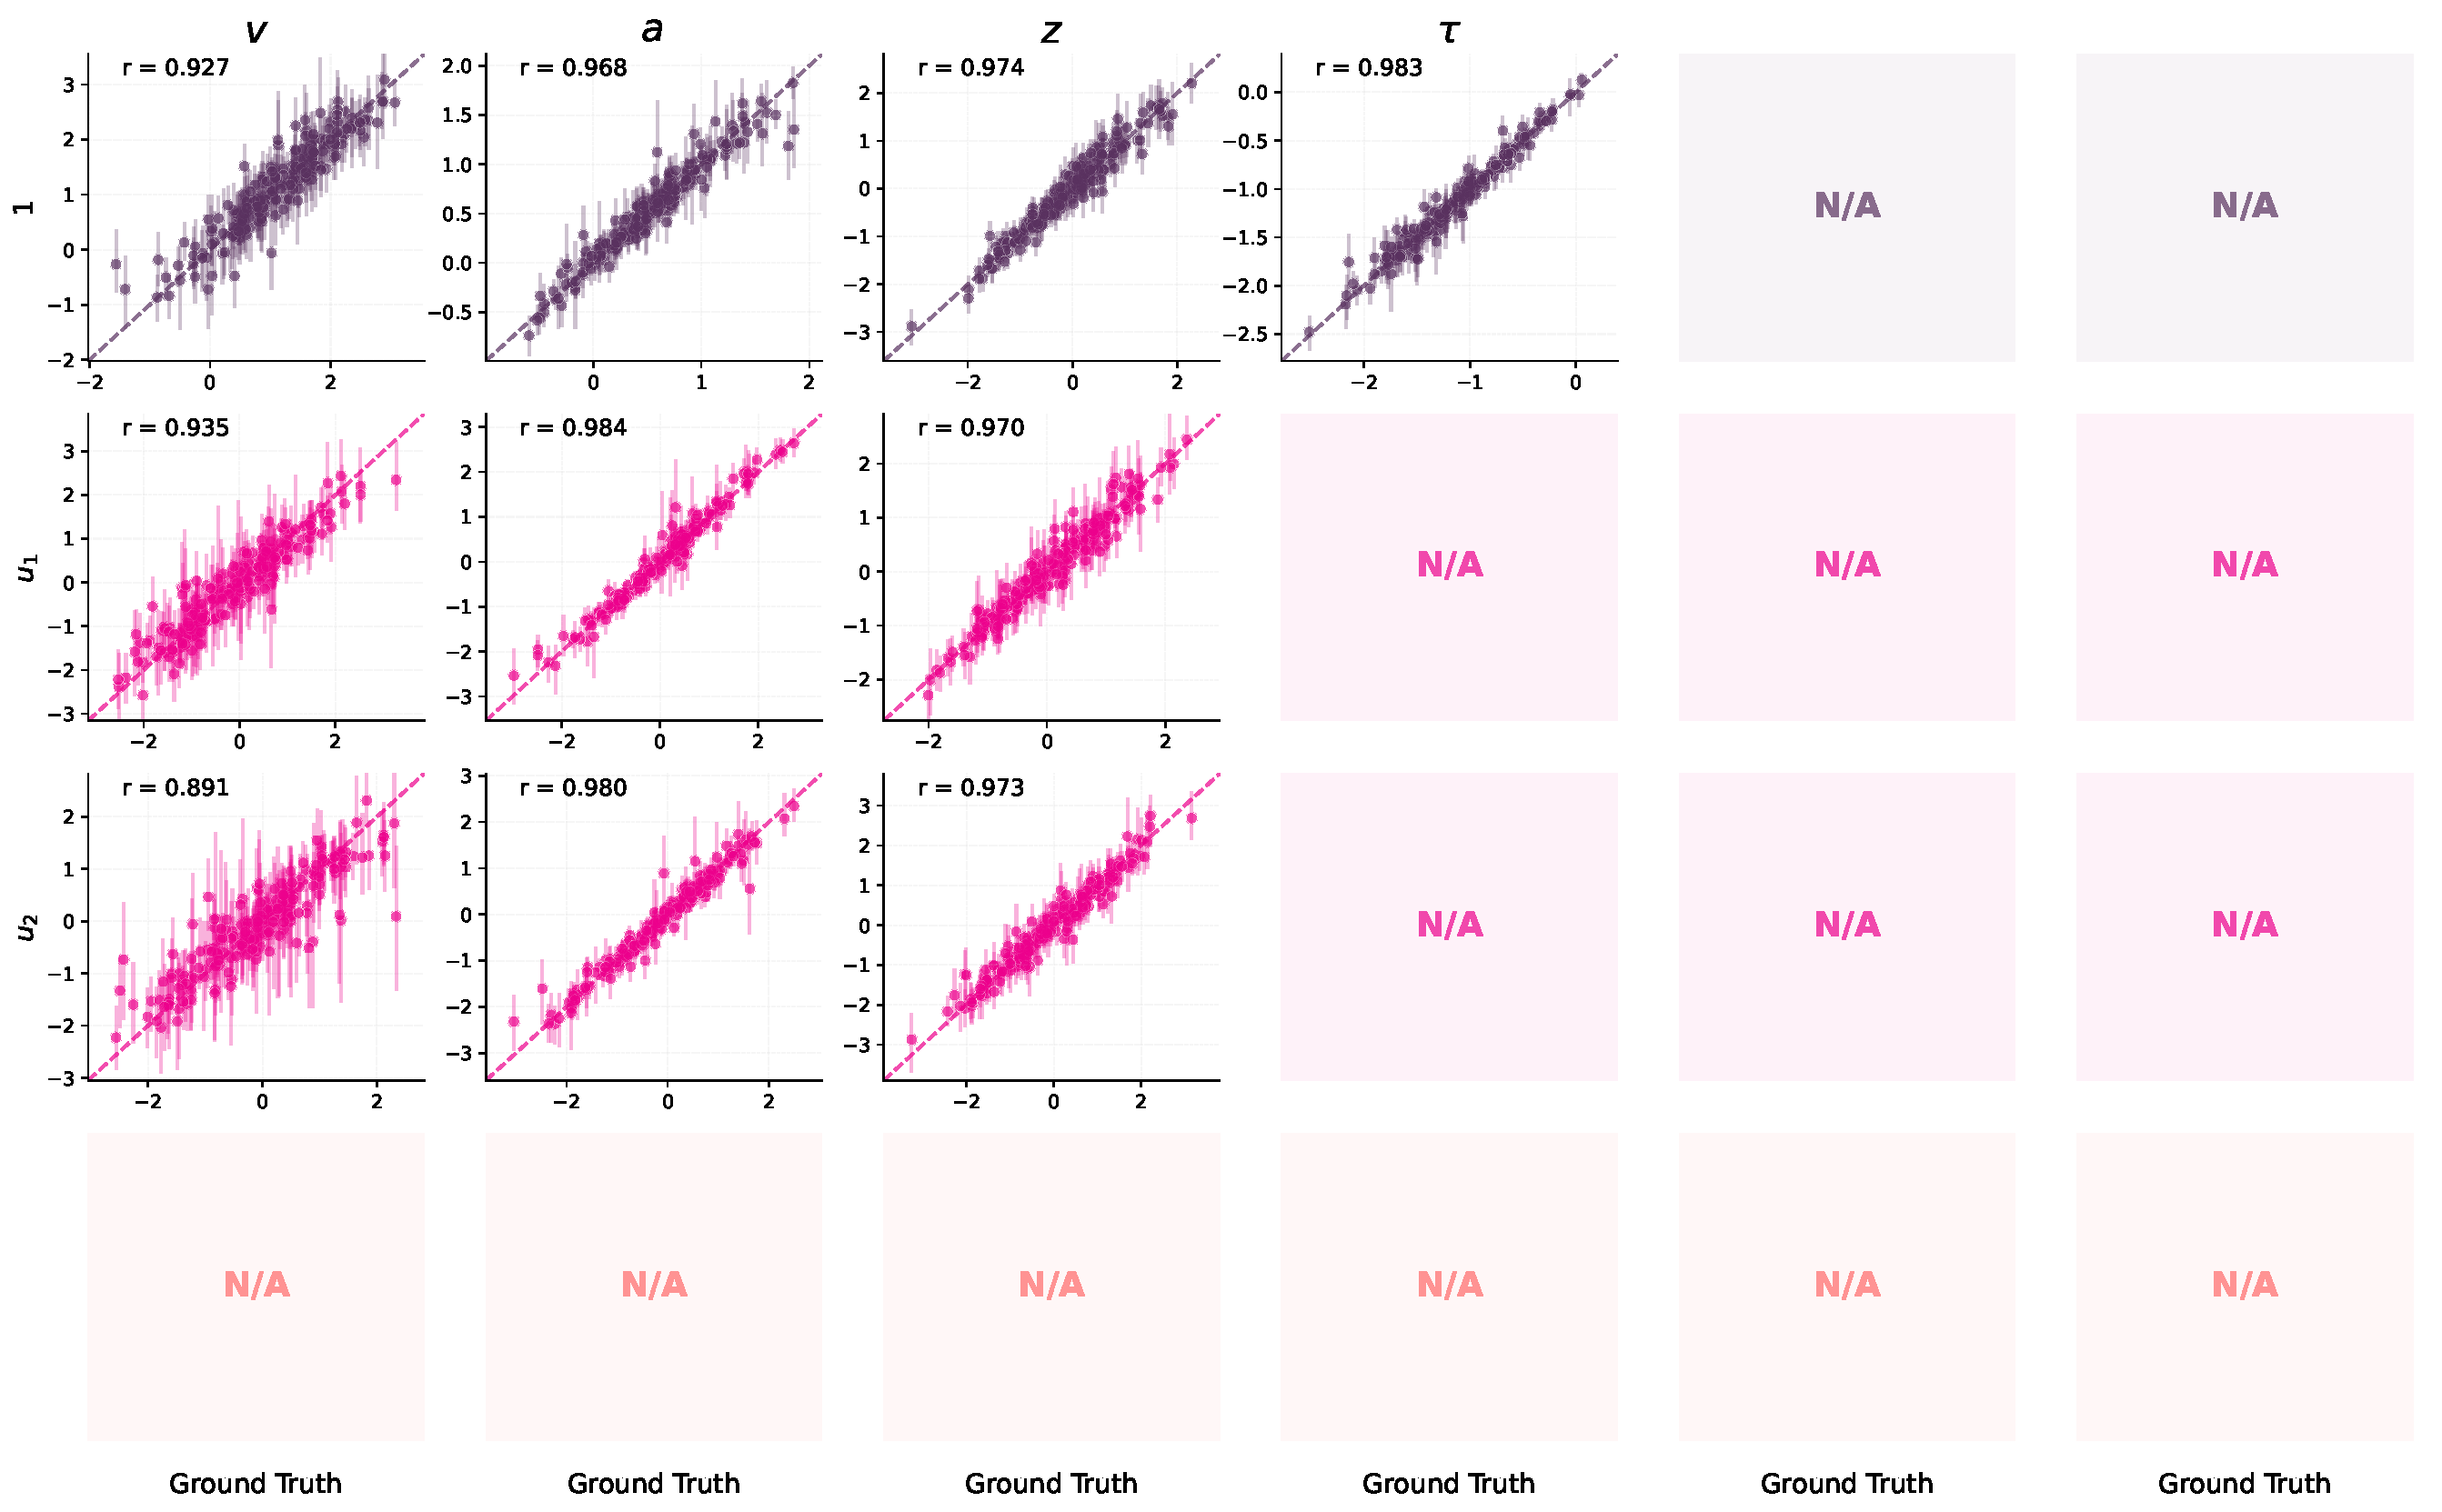
\includegraphics[width=0.99\linewidth]{figures/fm/ddm/fixed_regressed/ddm_family_fixed_regressed_fm_mixed_recovery.pdf}
    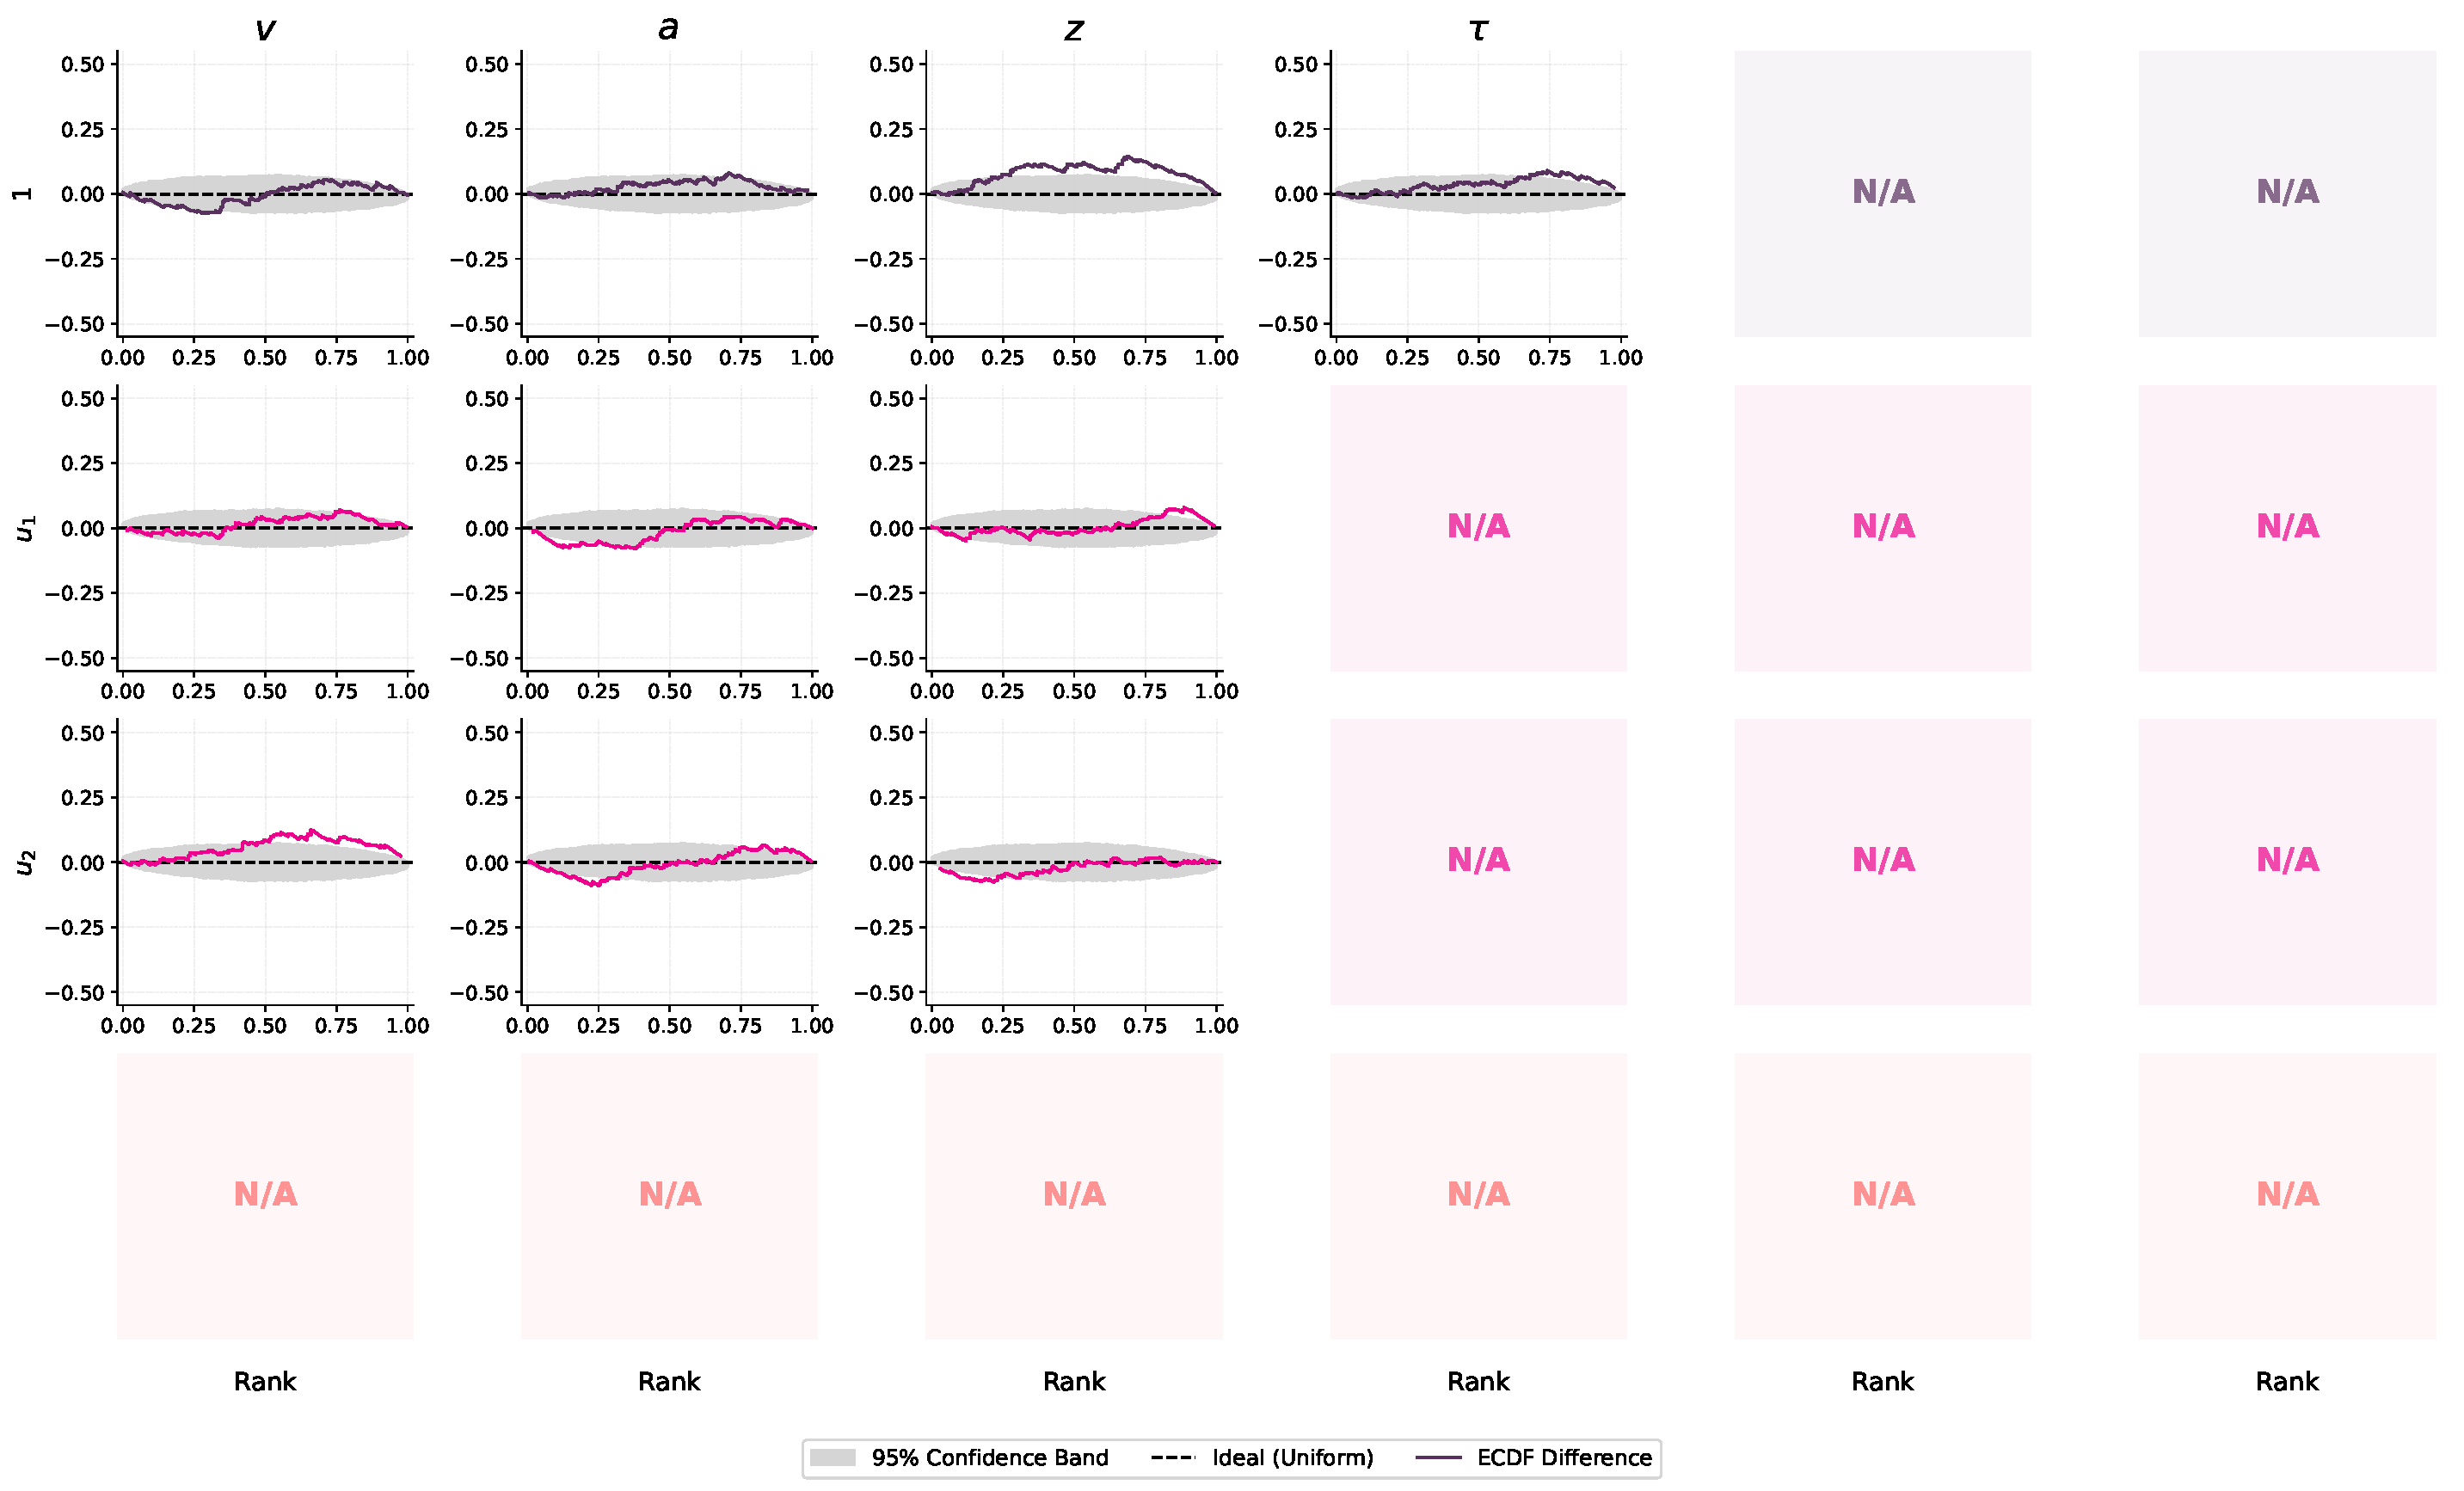
\includegraphics[width=0.99\linewidth]{figures/fm/ddm/fixed_regressed/ddm_family_fixed_regressed_fm_mixed_ecdf.pdf}
    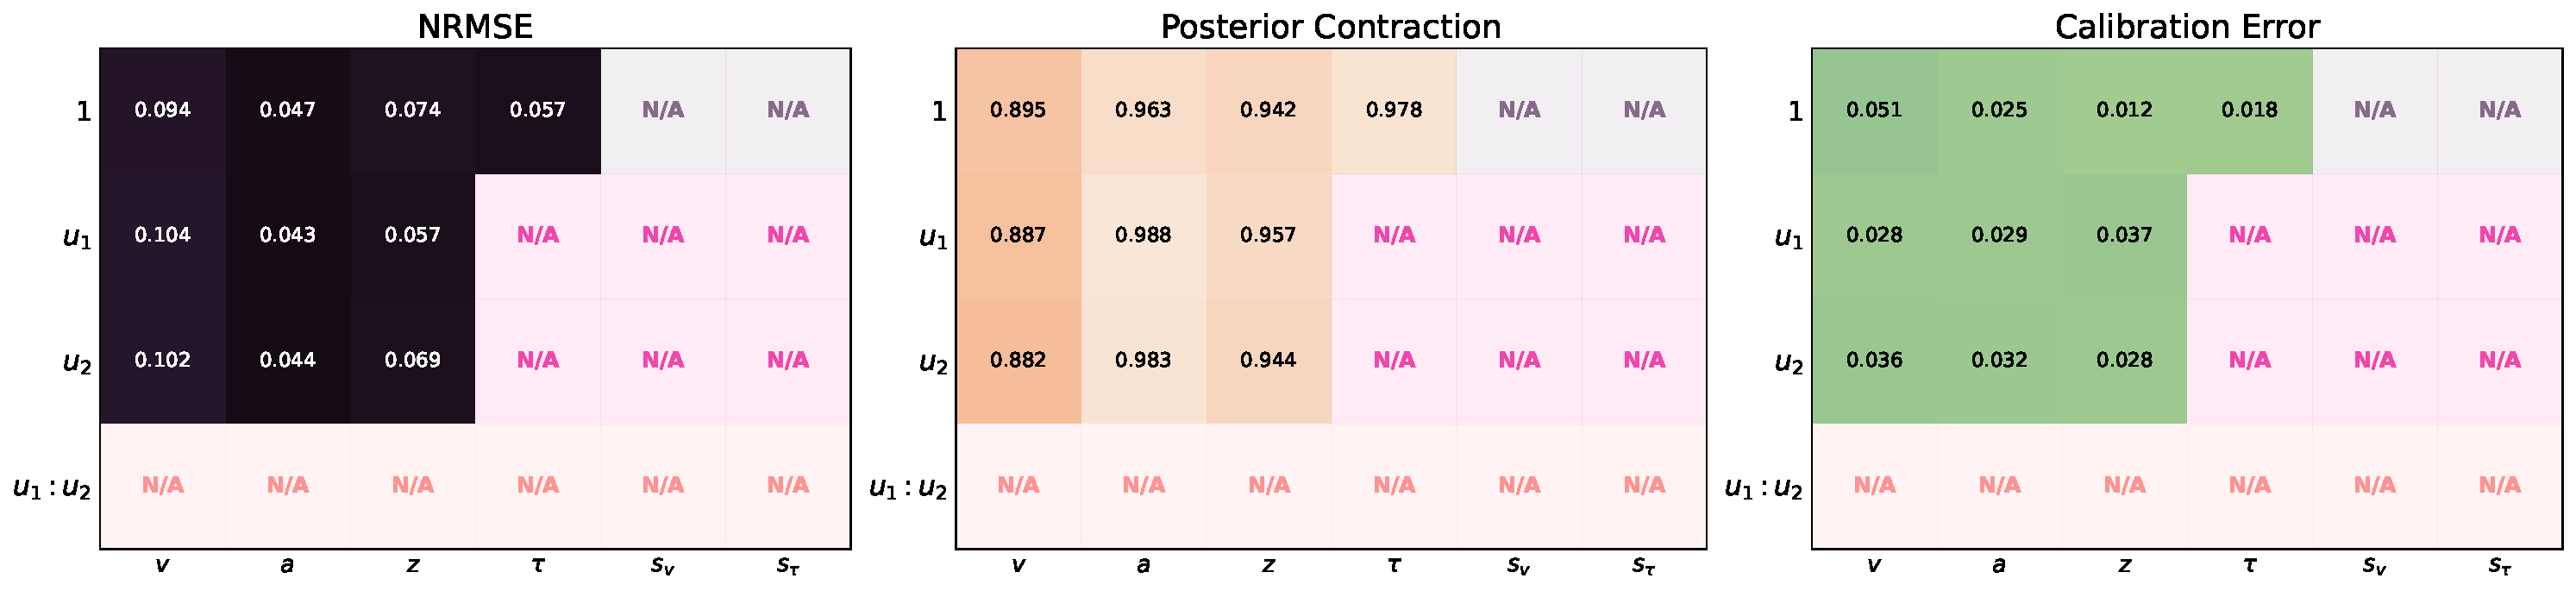
\includegraphics[width=0.99\linewidth]{figures/fm/ddm/fixed_regressed/ddm_family_fixed_regressed_fm_mixed_metrics.pdf}
    \caption{Parameter recovery (\emph{top}), calibration ECDF (\emph{middle}), and parameter-wise metrics (NRMSE, calibration error, and posterior contraction) for DDM model family (Case \textbf{fixed\_regressed}).}
    \label{fig:ddm-fm-fixed-regressed}
\end{figure}

\begin{figure}
    \centering
    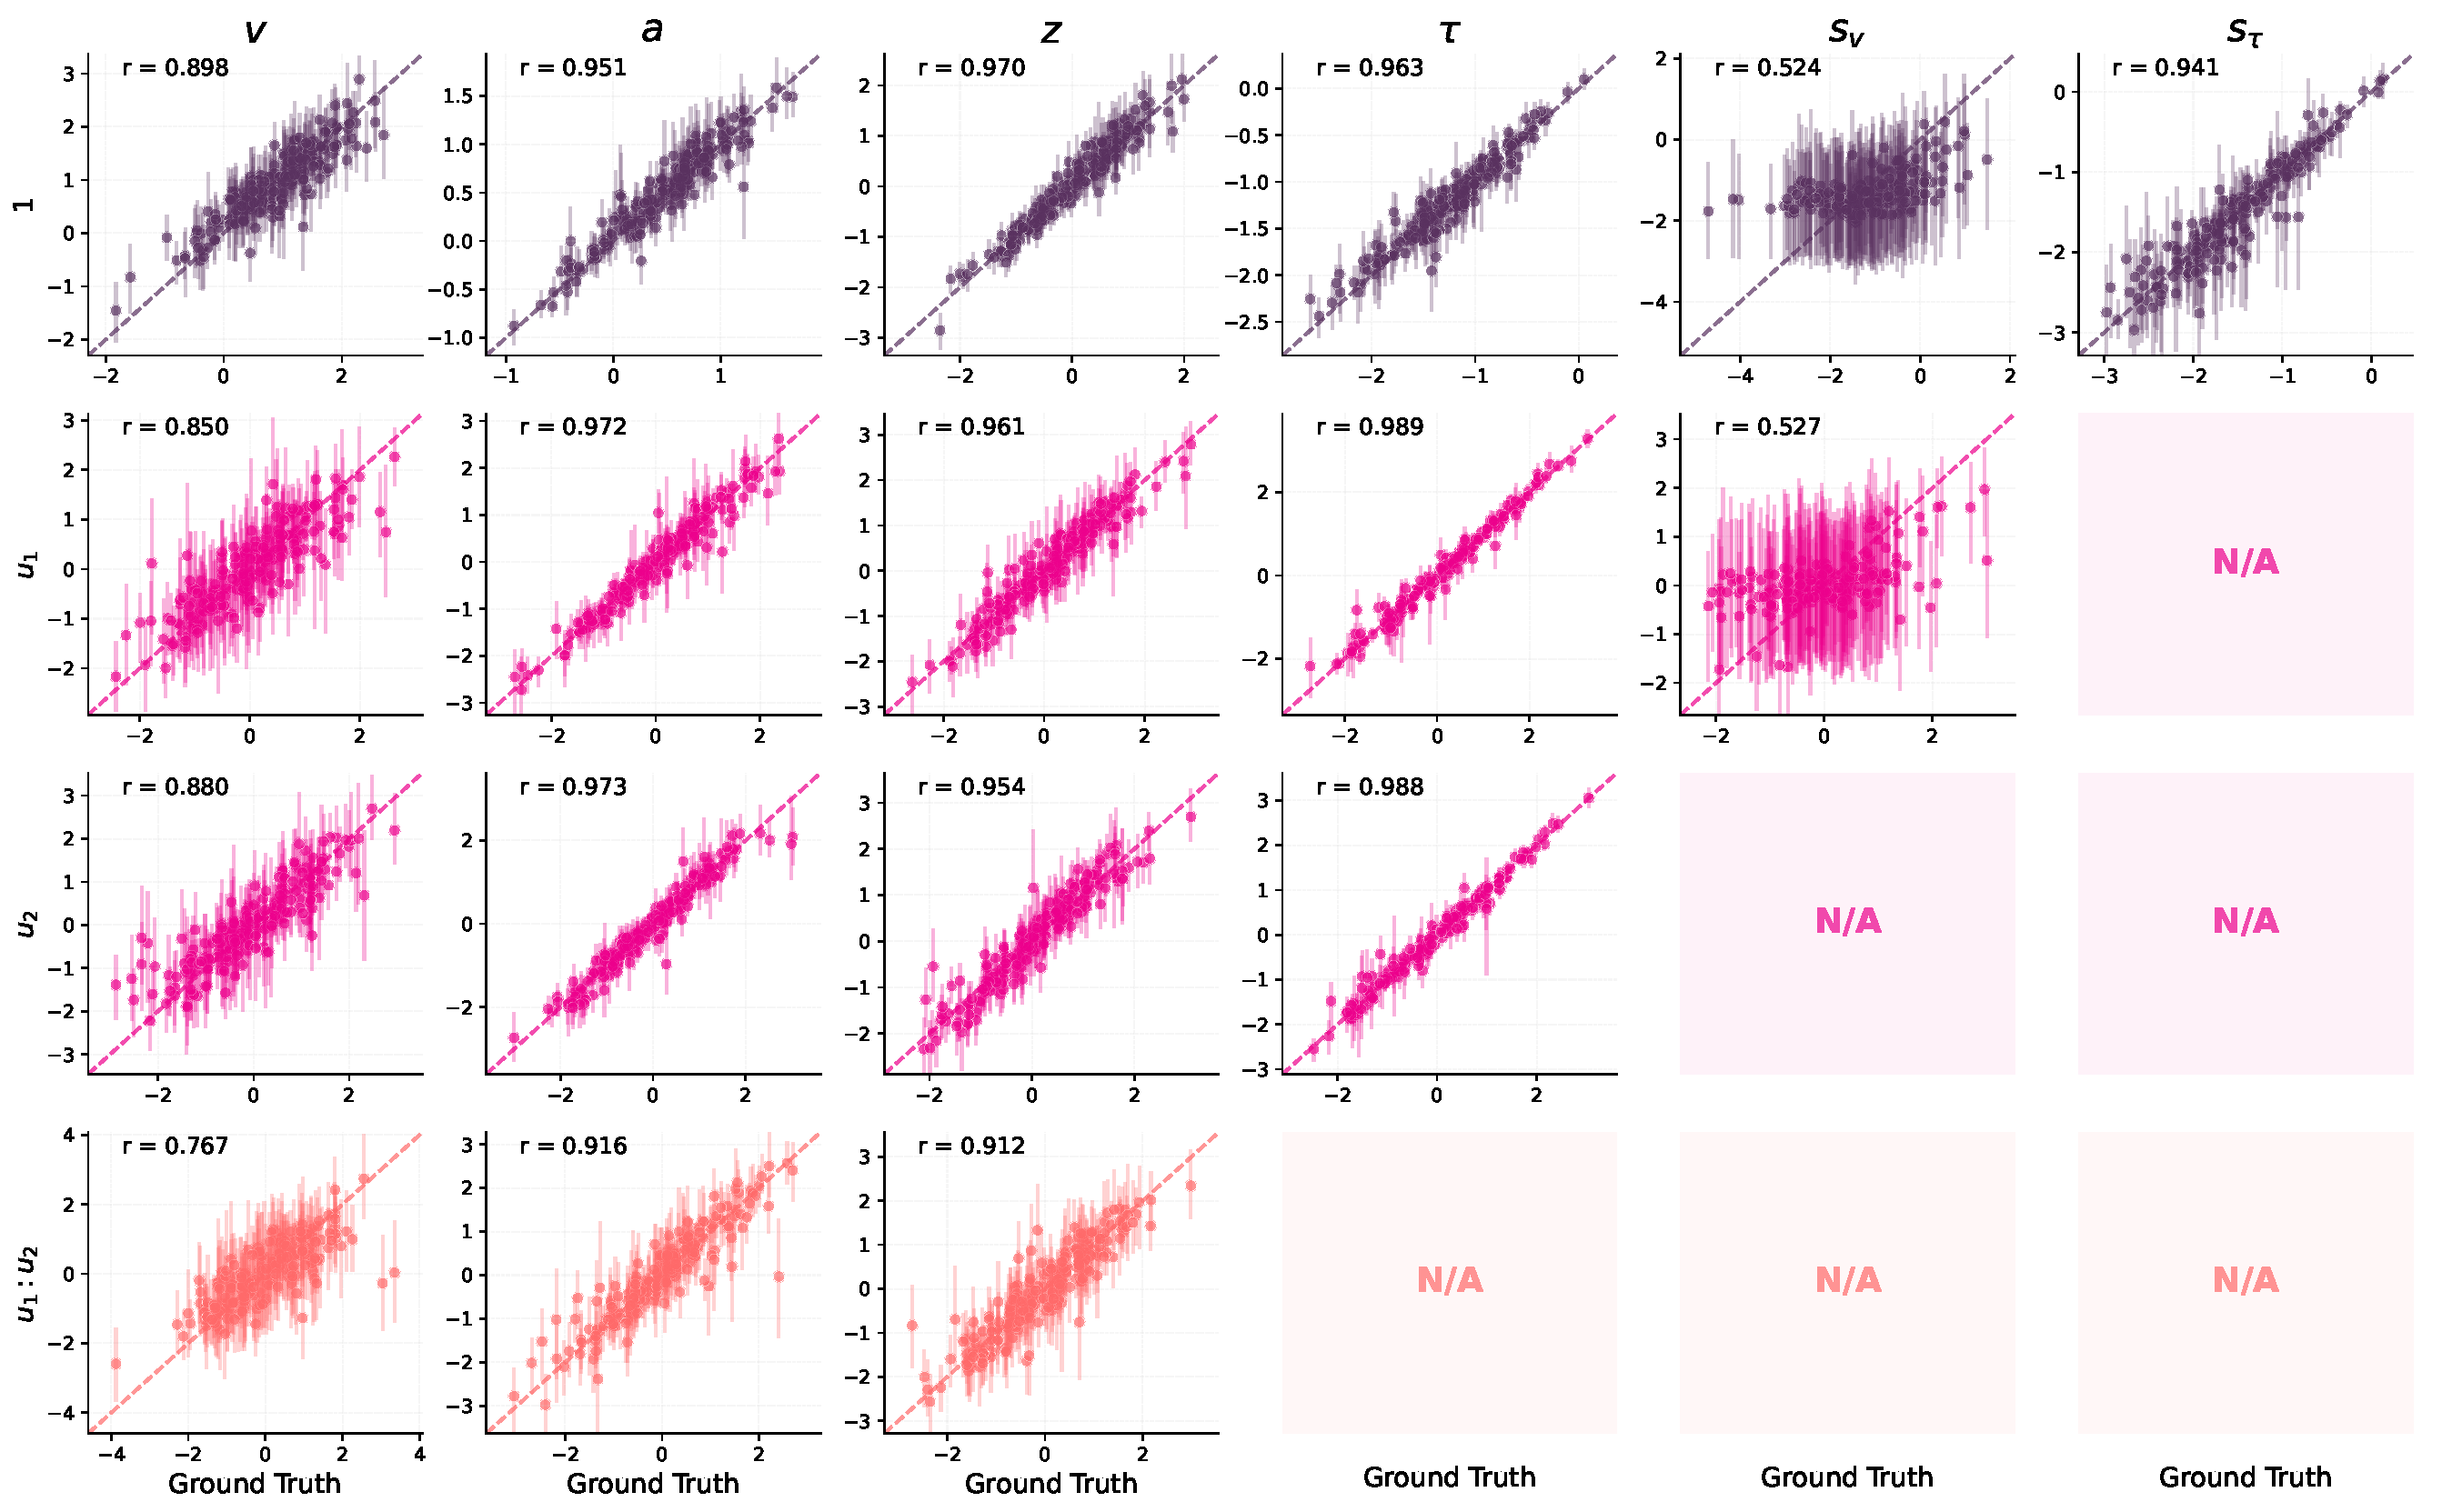
\includegraphics[width=0.99\linewidth]{figures/fm/ddm/interaction/ddm_family_interaction_fm_mixed_recovery.pdf}
    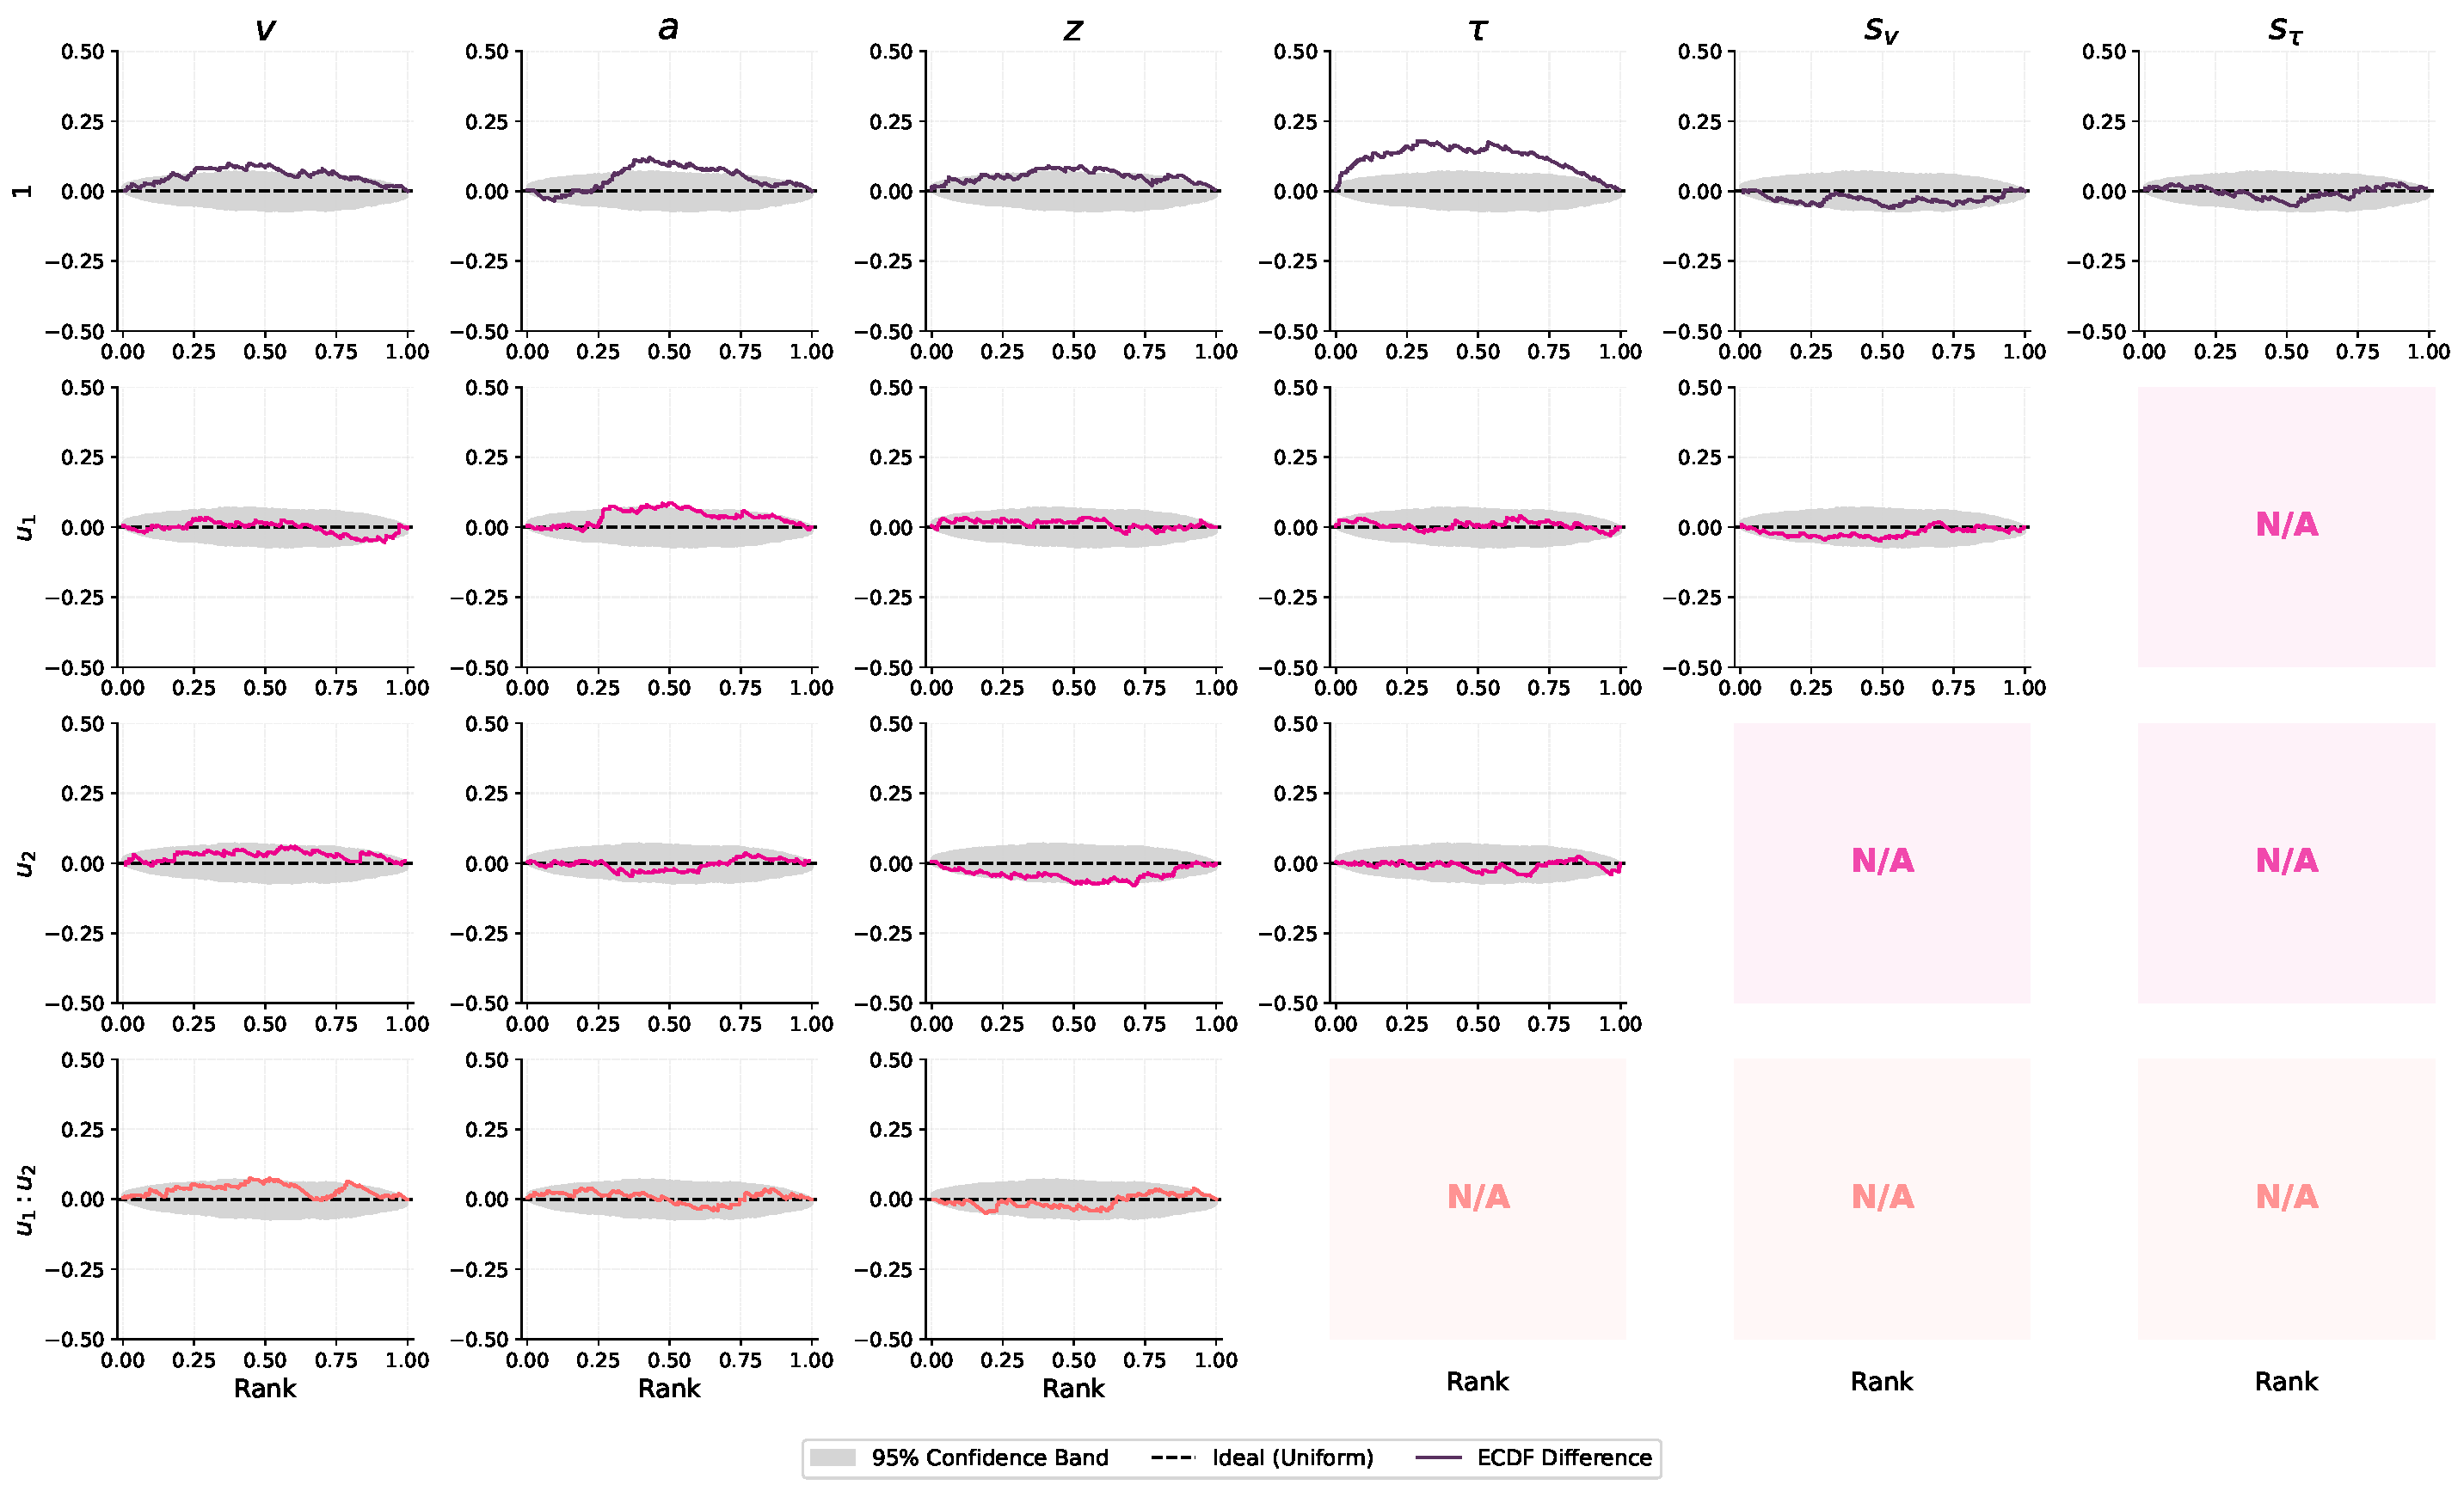
\includegraphics[width=0.99\linewidth]{figures/fm/ddm/interaction/ddm_family_interaction_fm_mixed_ecdf.pdf}
    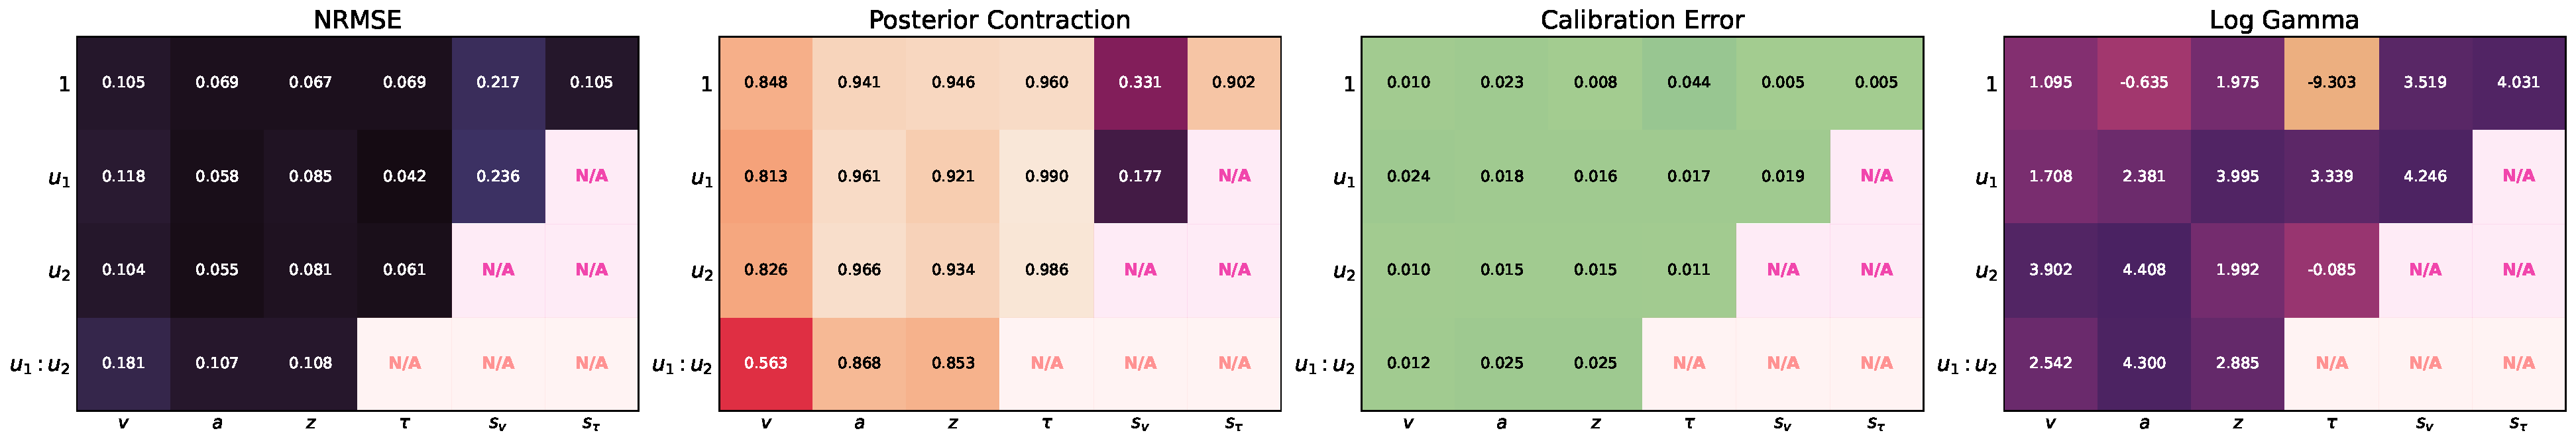
\includegraphics[width=0.99\linewidth]{figures/fm/ddm/interaction/ddm_family_interaction_fm_mixed_metrics.pdf}
    \caption{Parameter recovery (\emph{top}), calibration ECDF (\emph{middle}), and parameter-wise metrics (NRMSE, calibration error, and posterior contraction) for DDM model family (Case \textbf{interaction}).}
    \label{fig:ddm-fm-interaction}
\end{figure}

% ========================================
% RDM BASELINE (bf)
% ========================================

\begin{figure}
    \centering
    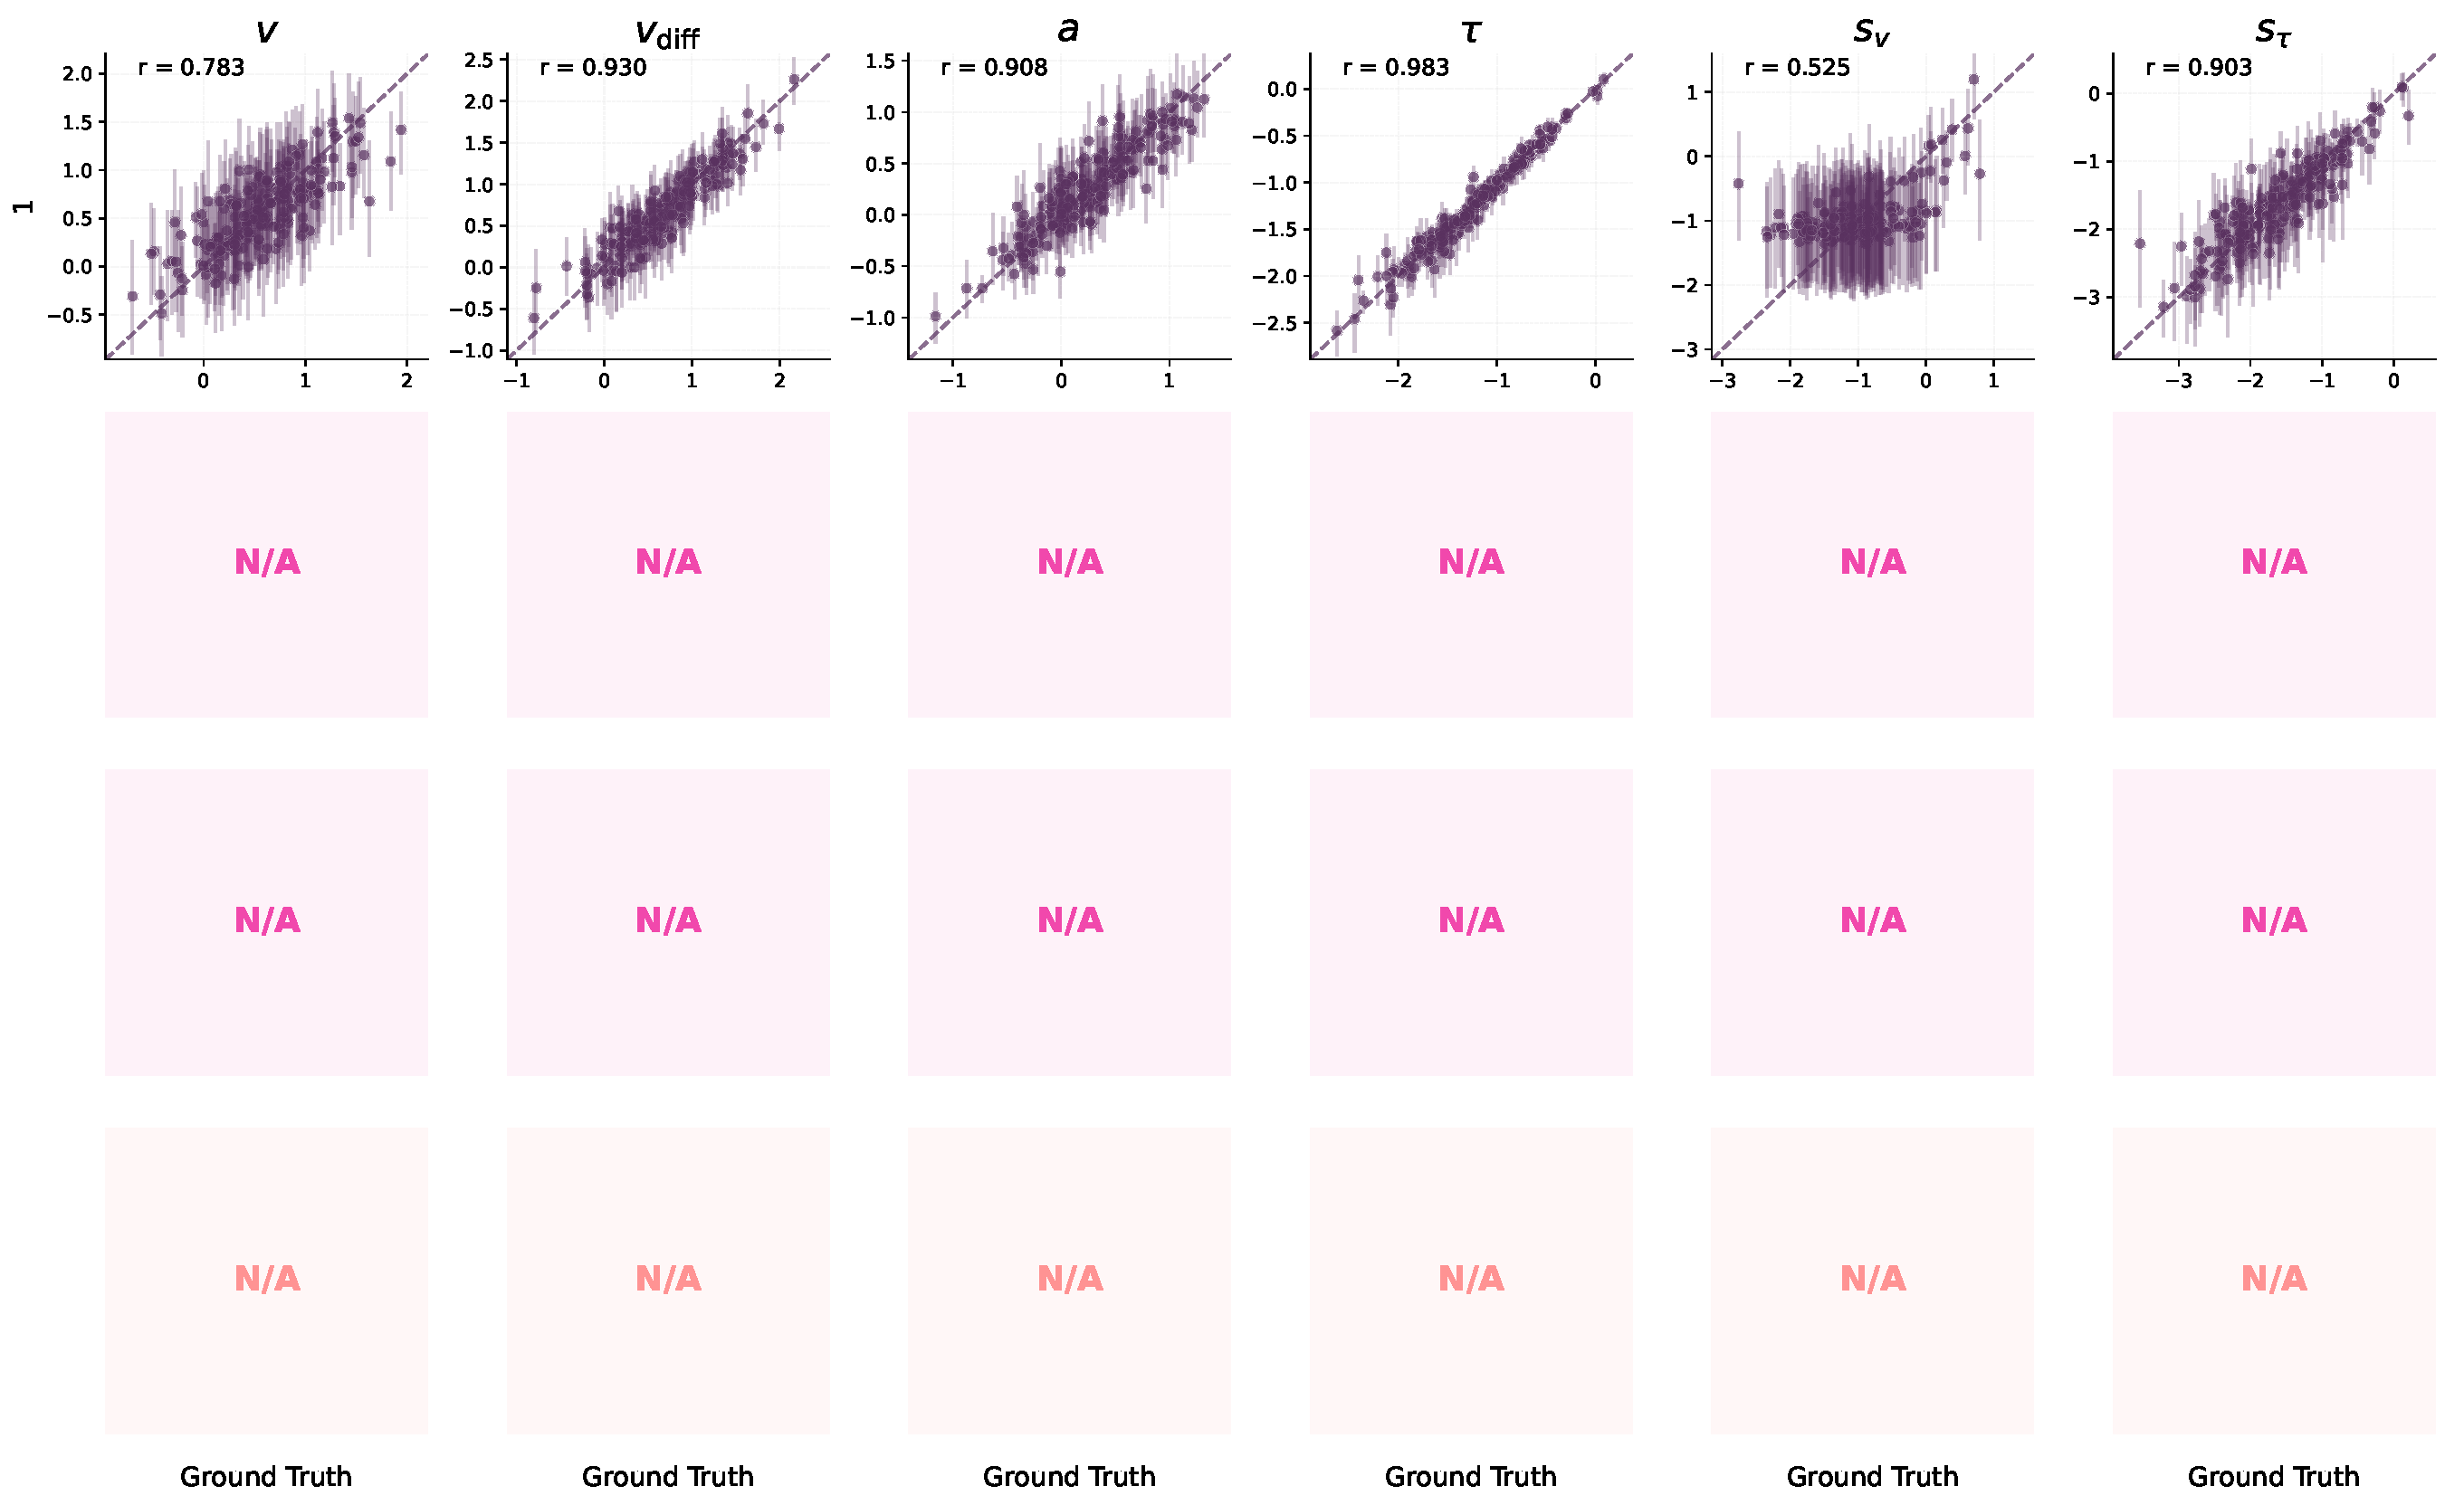
\includegraphics[width=0.99\linewidth]{figures/bf/rdm/intercept_only/rdm_family_intercept_only_bf_recovery.pdf}
    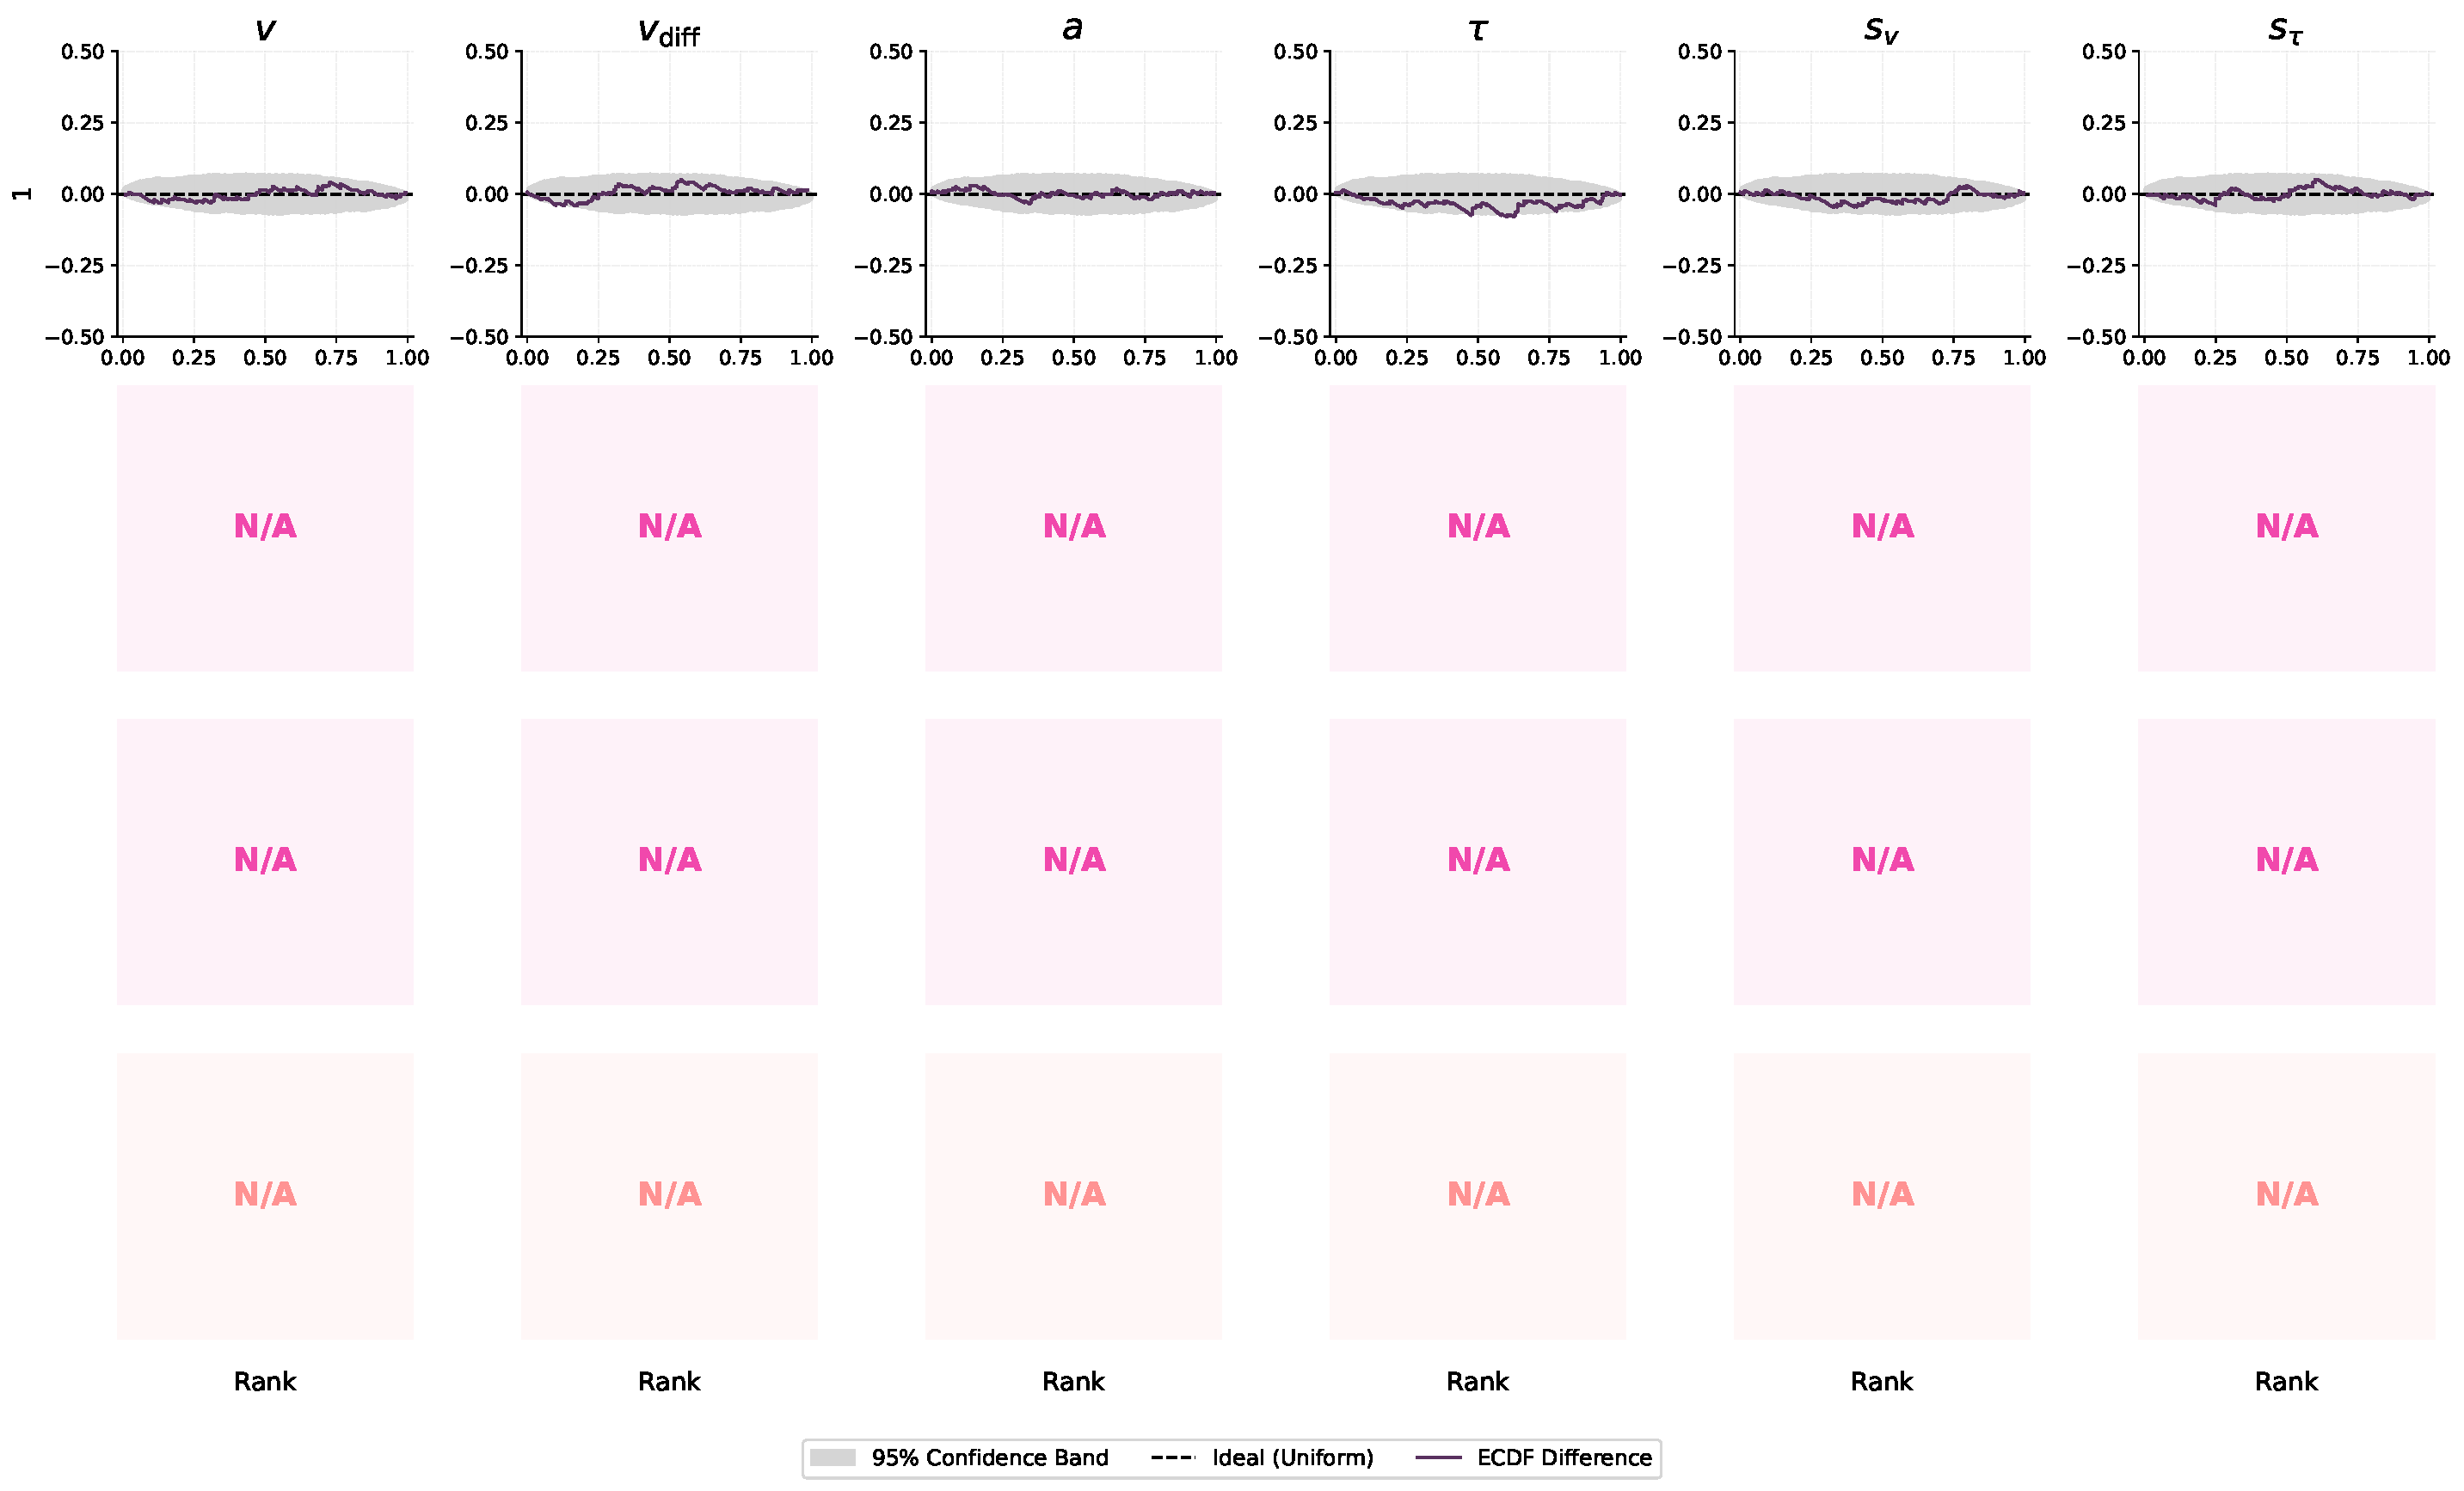
\includegraphics[width=0.99\linewidth]{figures/bf/rdm/intercept_only/rdm_family_intercept_only_bf_ecdf.pdf}
    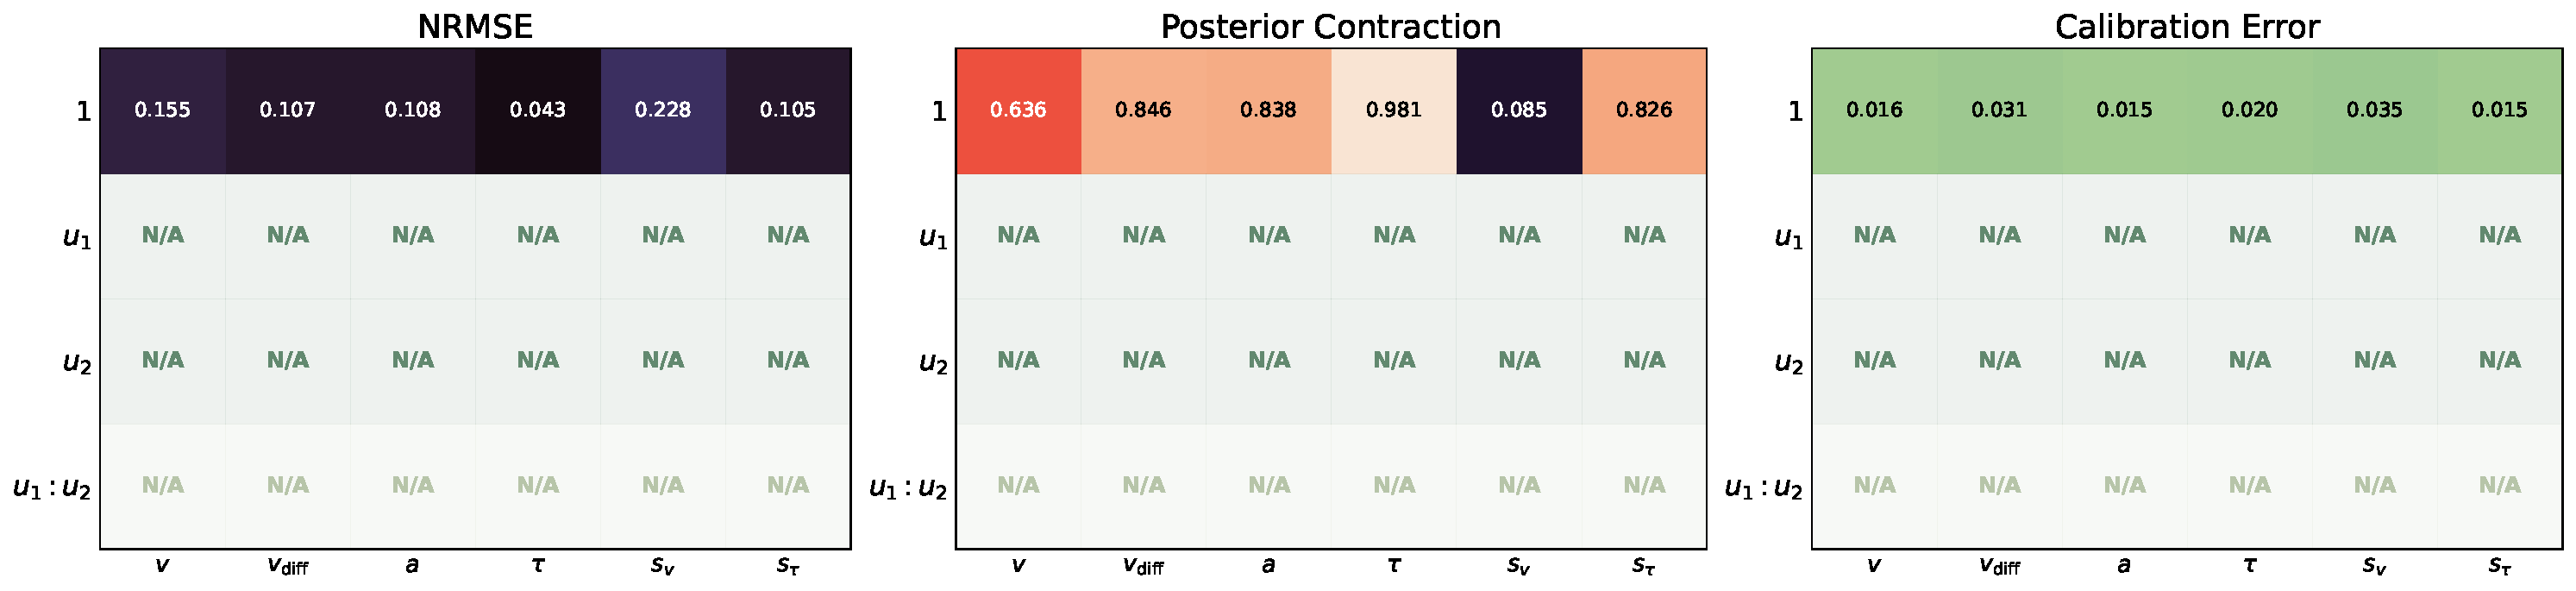
\includegraphics[width=0.99\linewidth]{figures/bf/rdm/intercept_only/rdm_family_intercept_only_bf_metrics.pdf}
    \caption{Parameter recovery (\emph{top}), calibration ECDF (\emph{middle}), and parameter-wise metrics (NRMSE, calibration error, and posterior contraction) for RDM baseline (Case \textbf{intercept\_only}).}
    \label{fig:rdm-bf-intercept-only}
\end{figure}

\begin{figure}
    \centering
    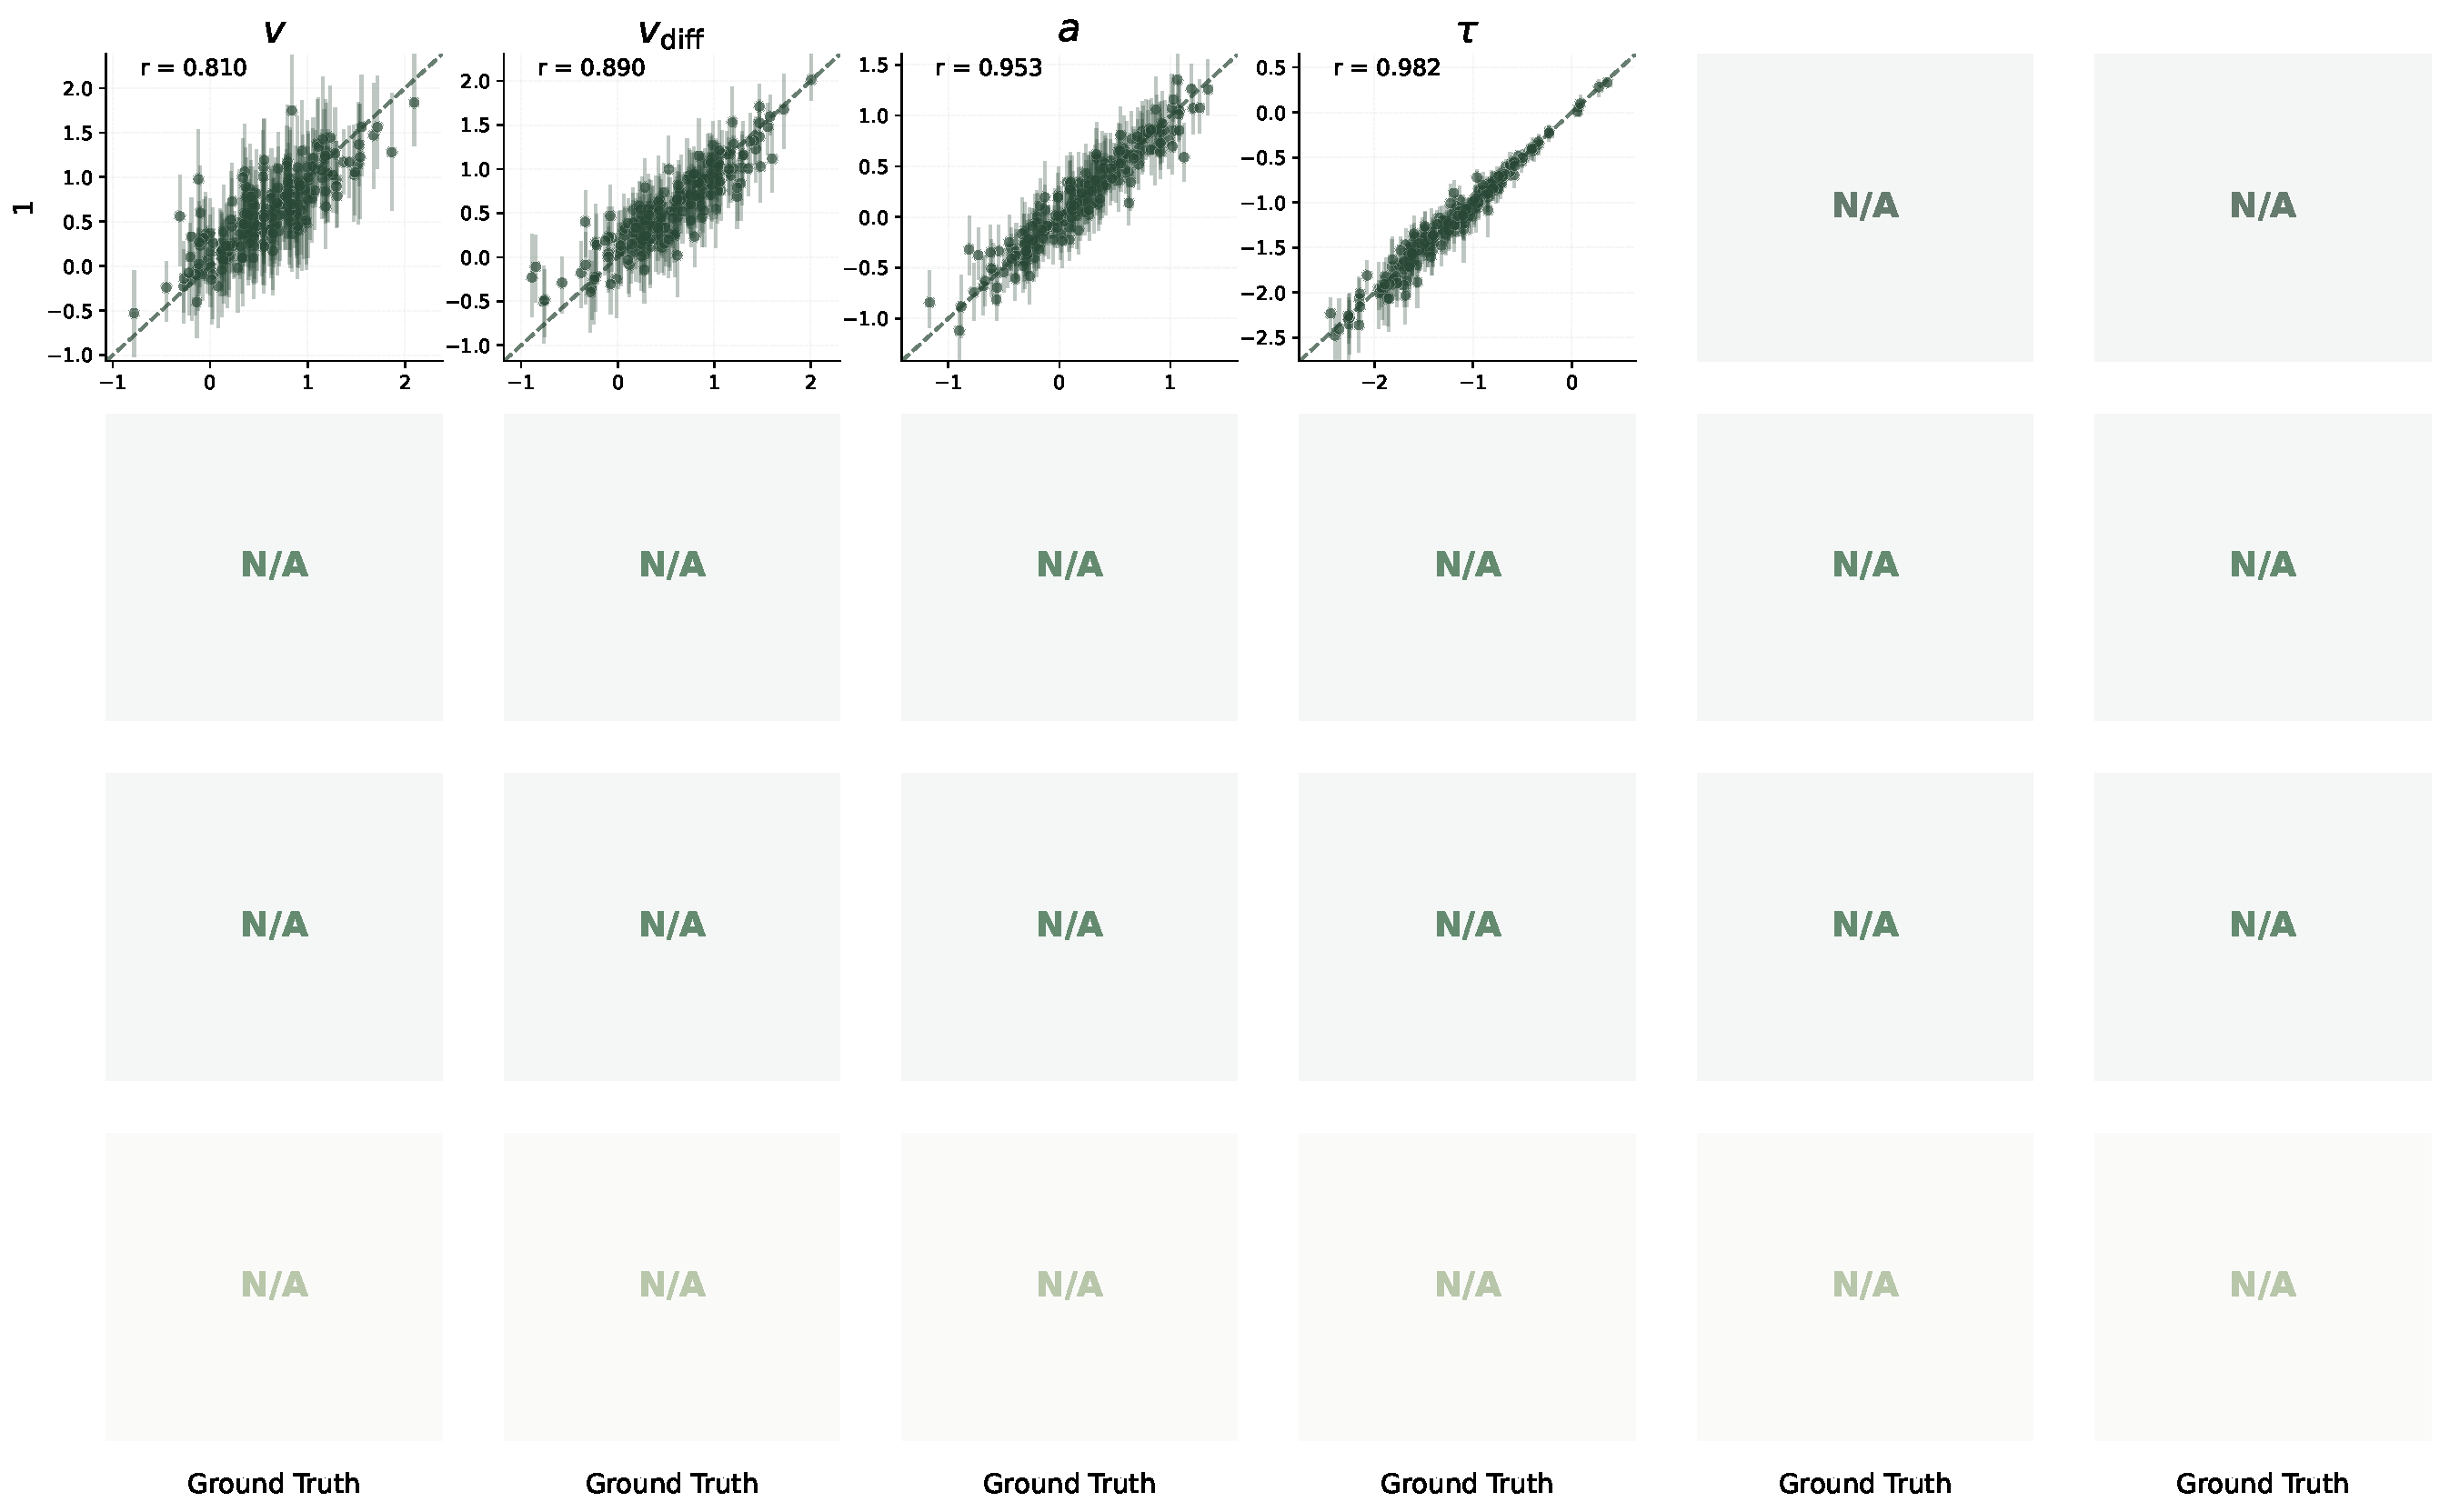
\includegraphics[width=0.99\linewidth]{figures/bf/rdm/fixed/rdm_family_fixed_bf_recovery.pdf}
    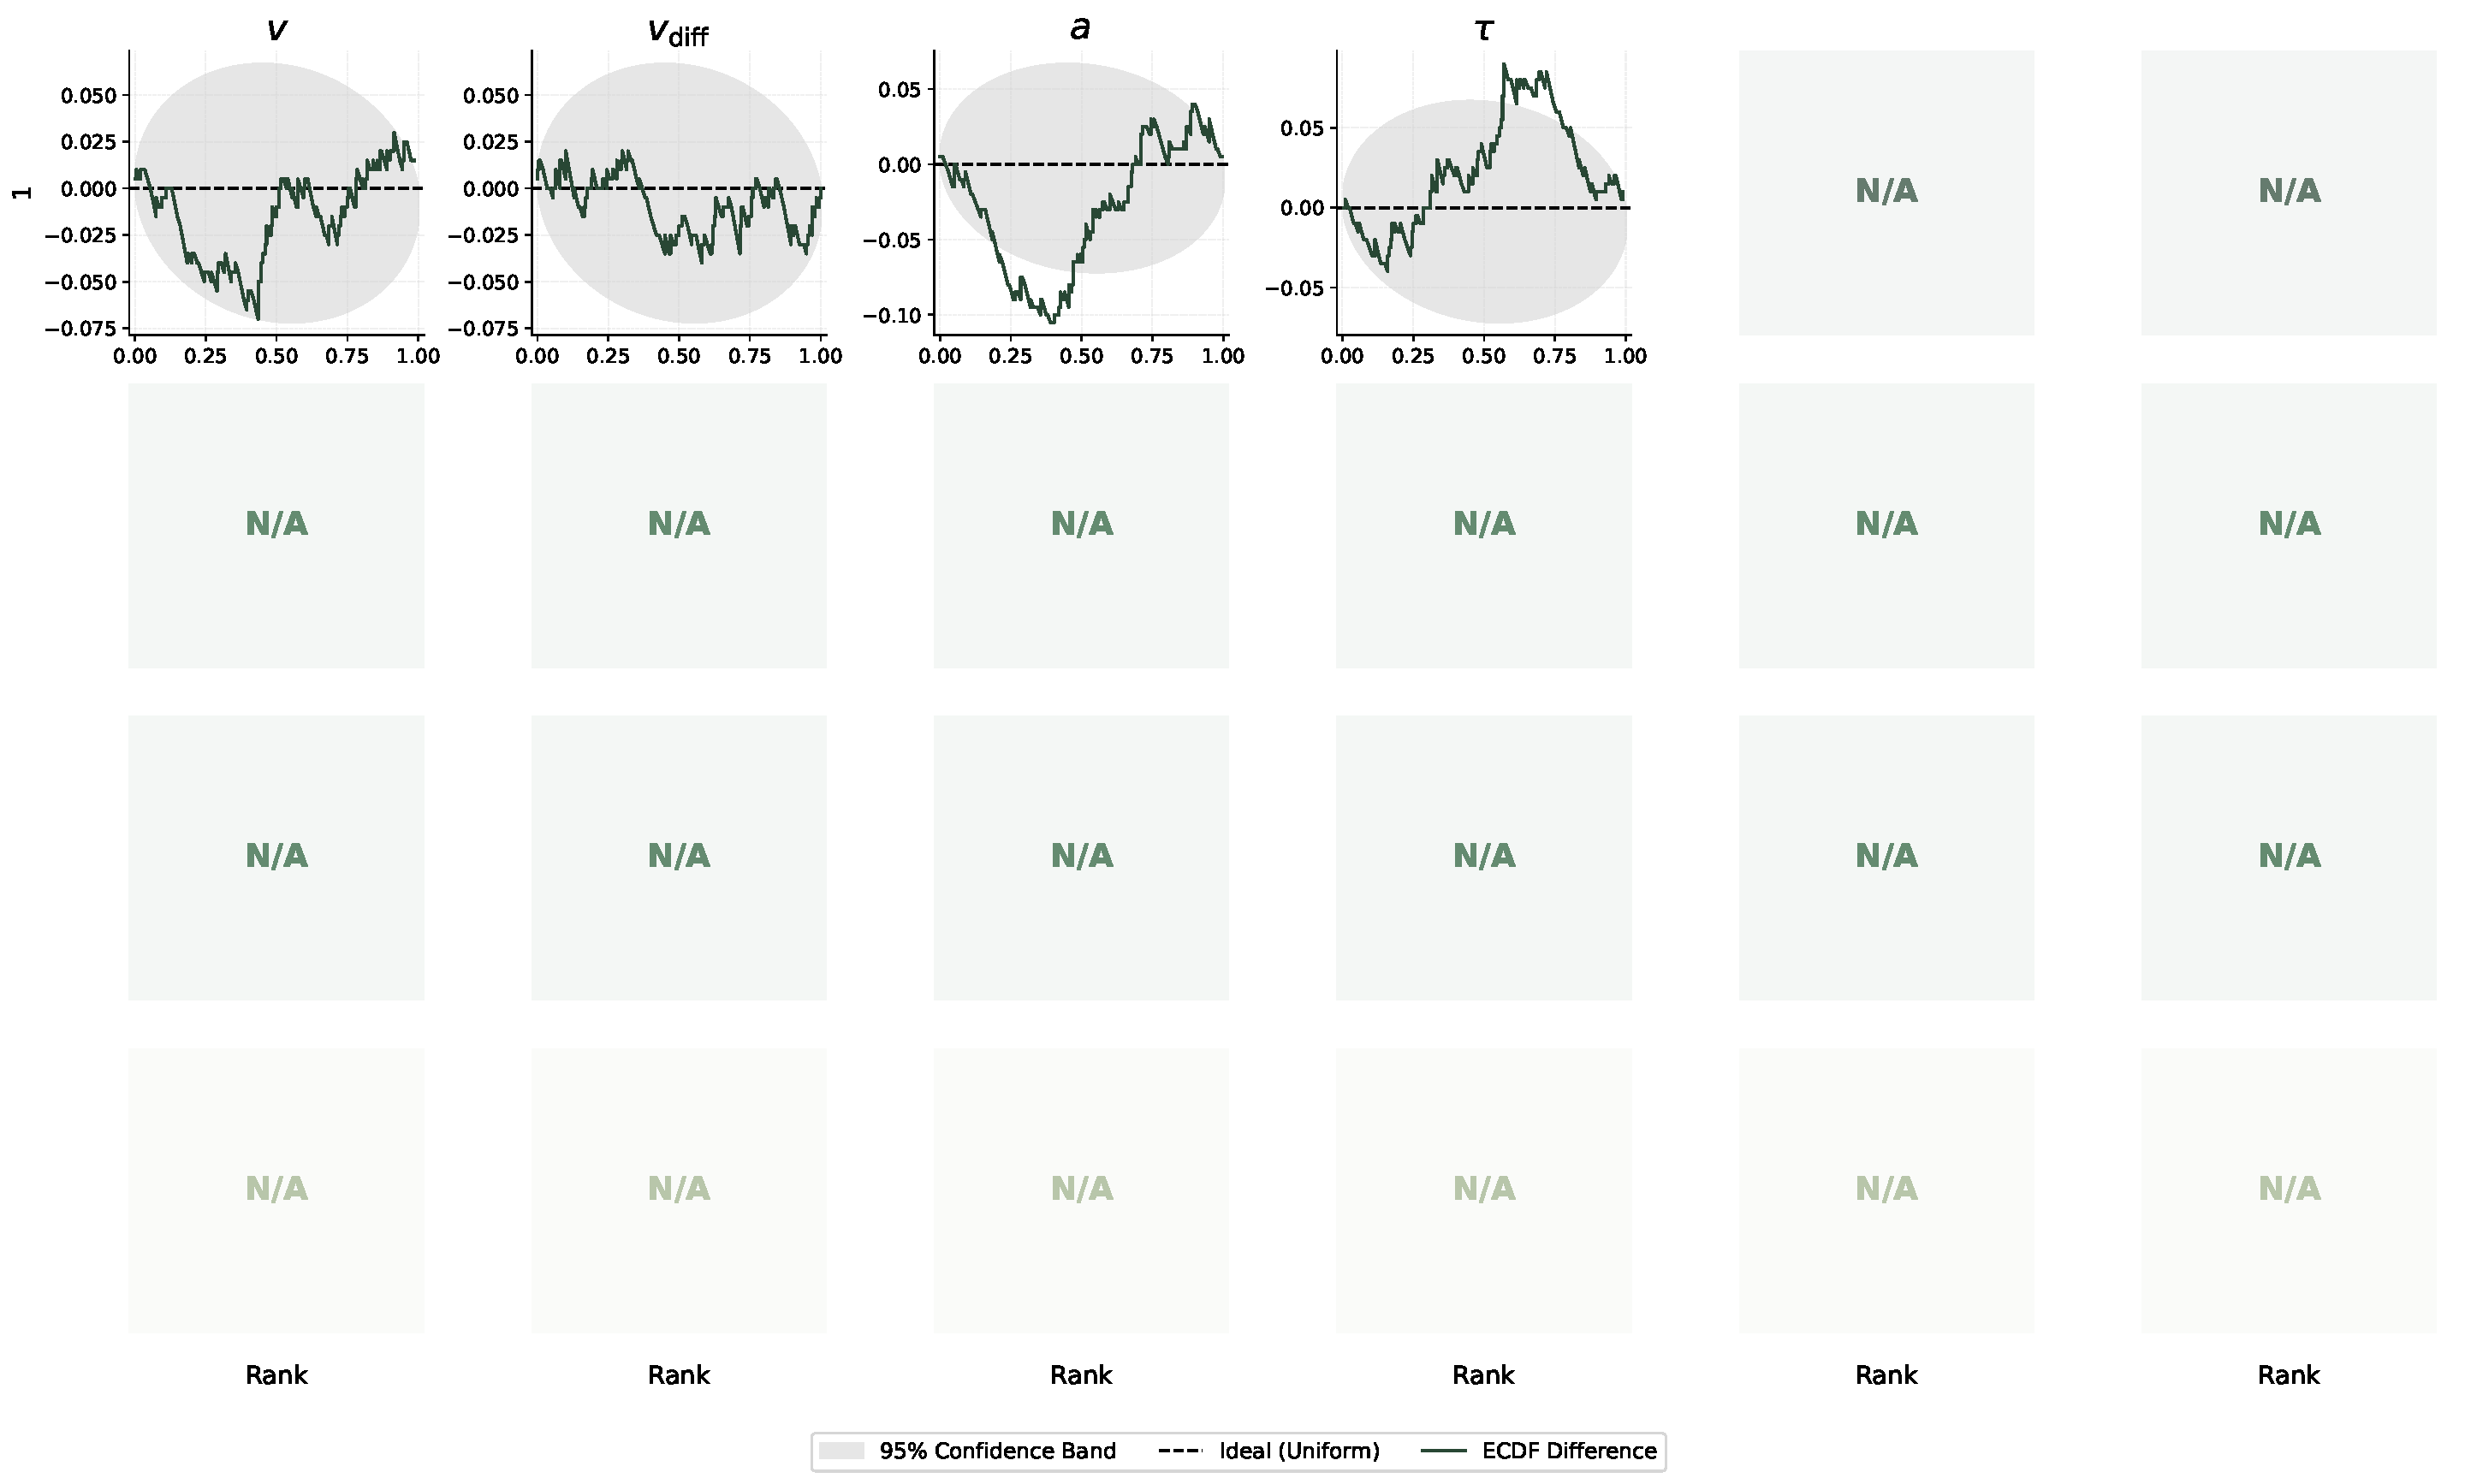
\includegraphics[width=0.99\linewidth]{figures/bf/rdm/fixed/rdm_family_fixed_bf_ecdf.pdf}
    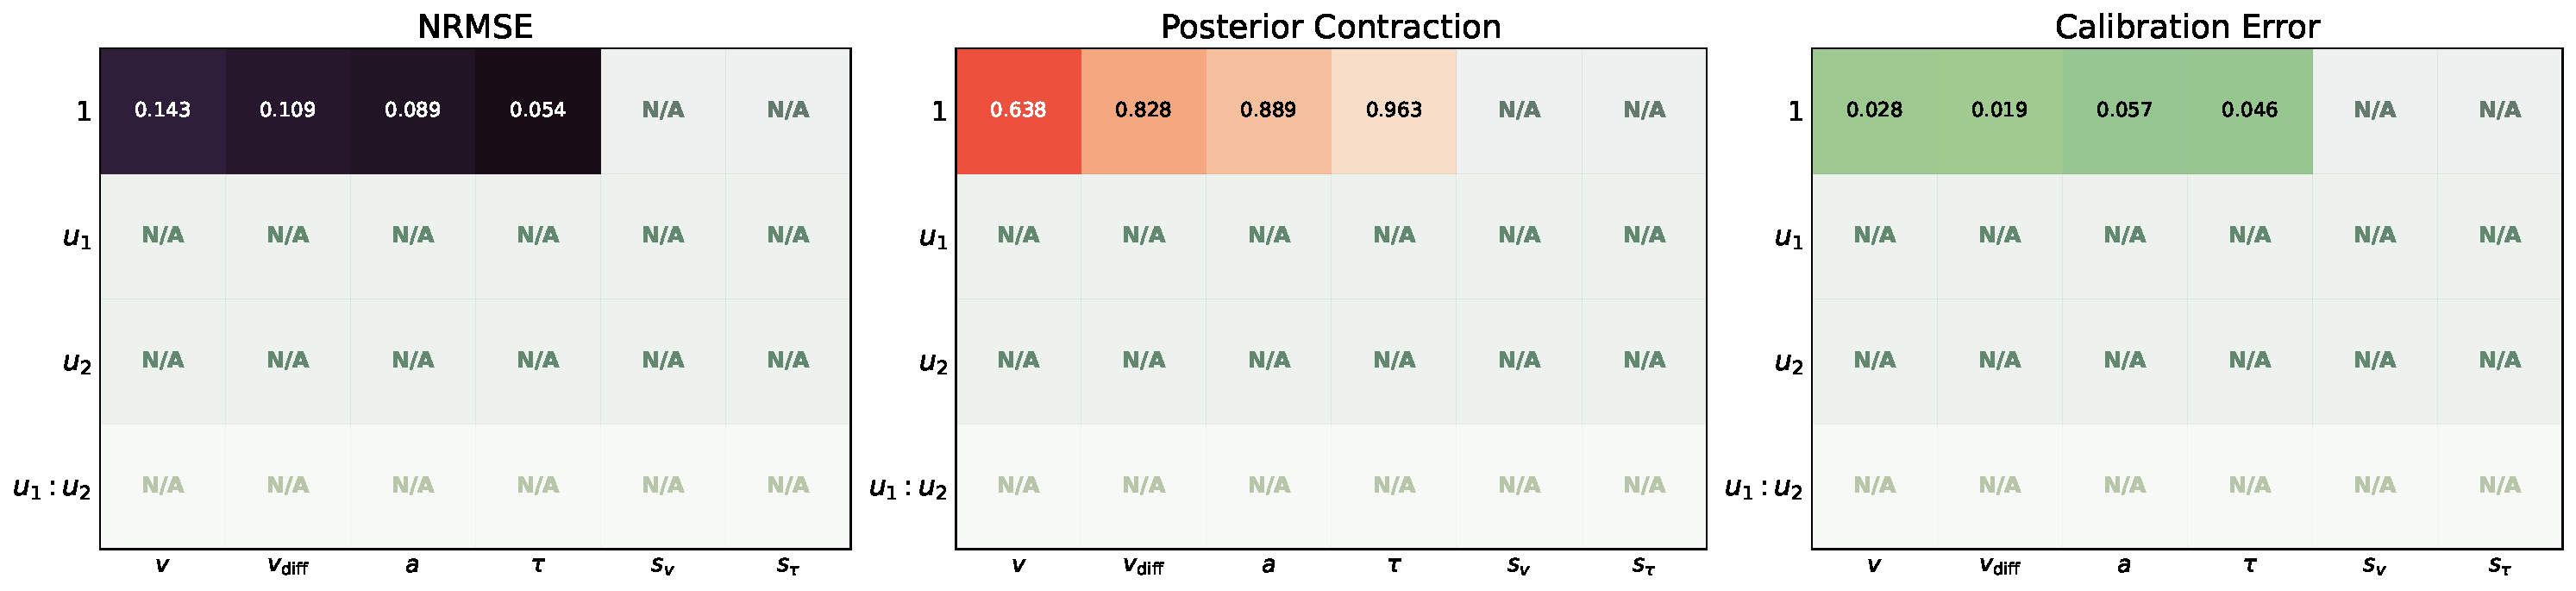
\includegraphics[width=0.99\linewidth]{figures/bf/rdm/fixed/rdm_family_fixed_bf_metrics.pdf}
    \caption{Parameter recovery (\emph{top}), calibration ECDF (\emph{middle}), and parameter-wise metrics (NRMSE, calibration error, and posterior contraction) for RDM baseline (Case \textbf{fixed}).}
    \label{fig:rdm-bf-fixed}
\end{figure}

\begin{figure}
    \centering
    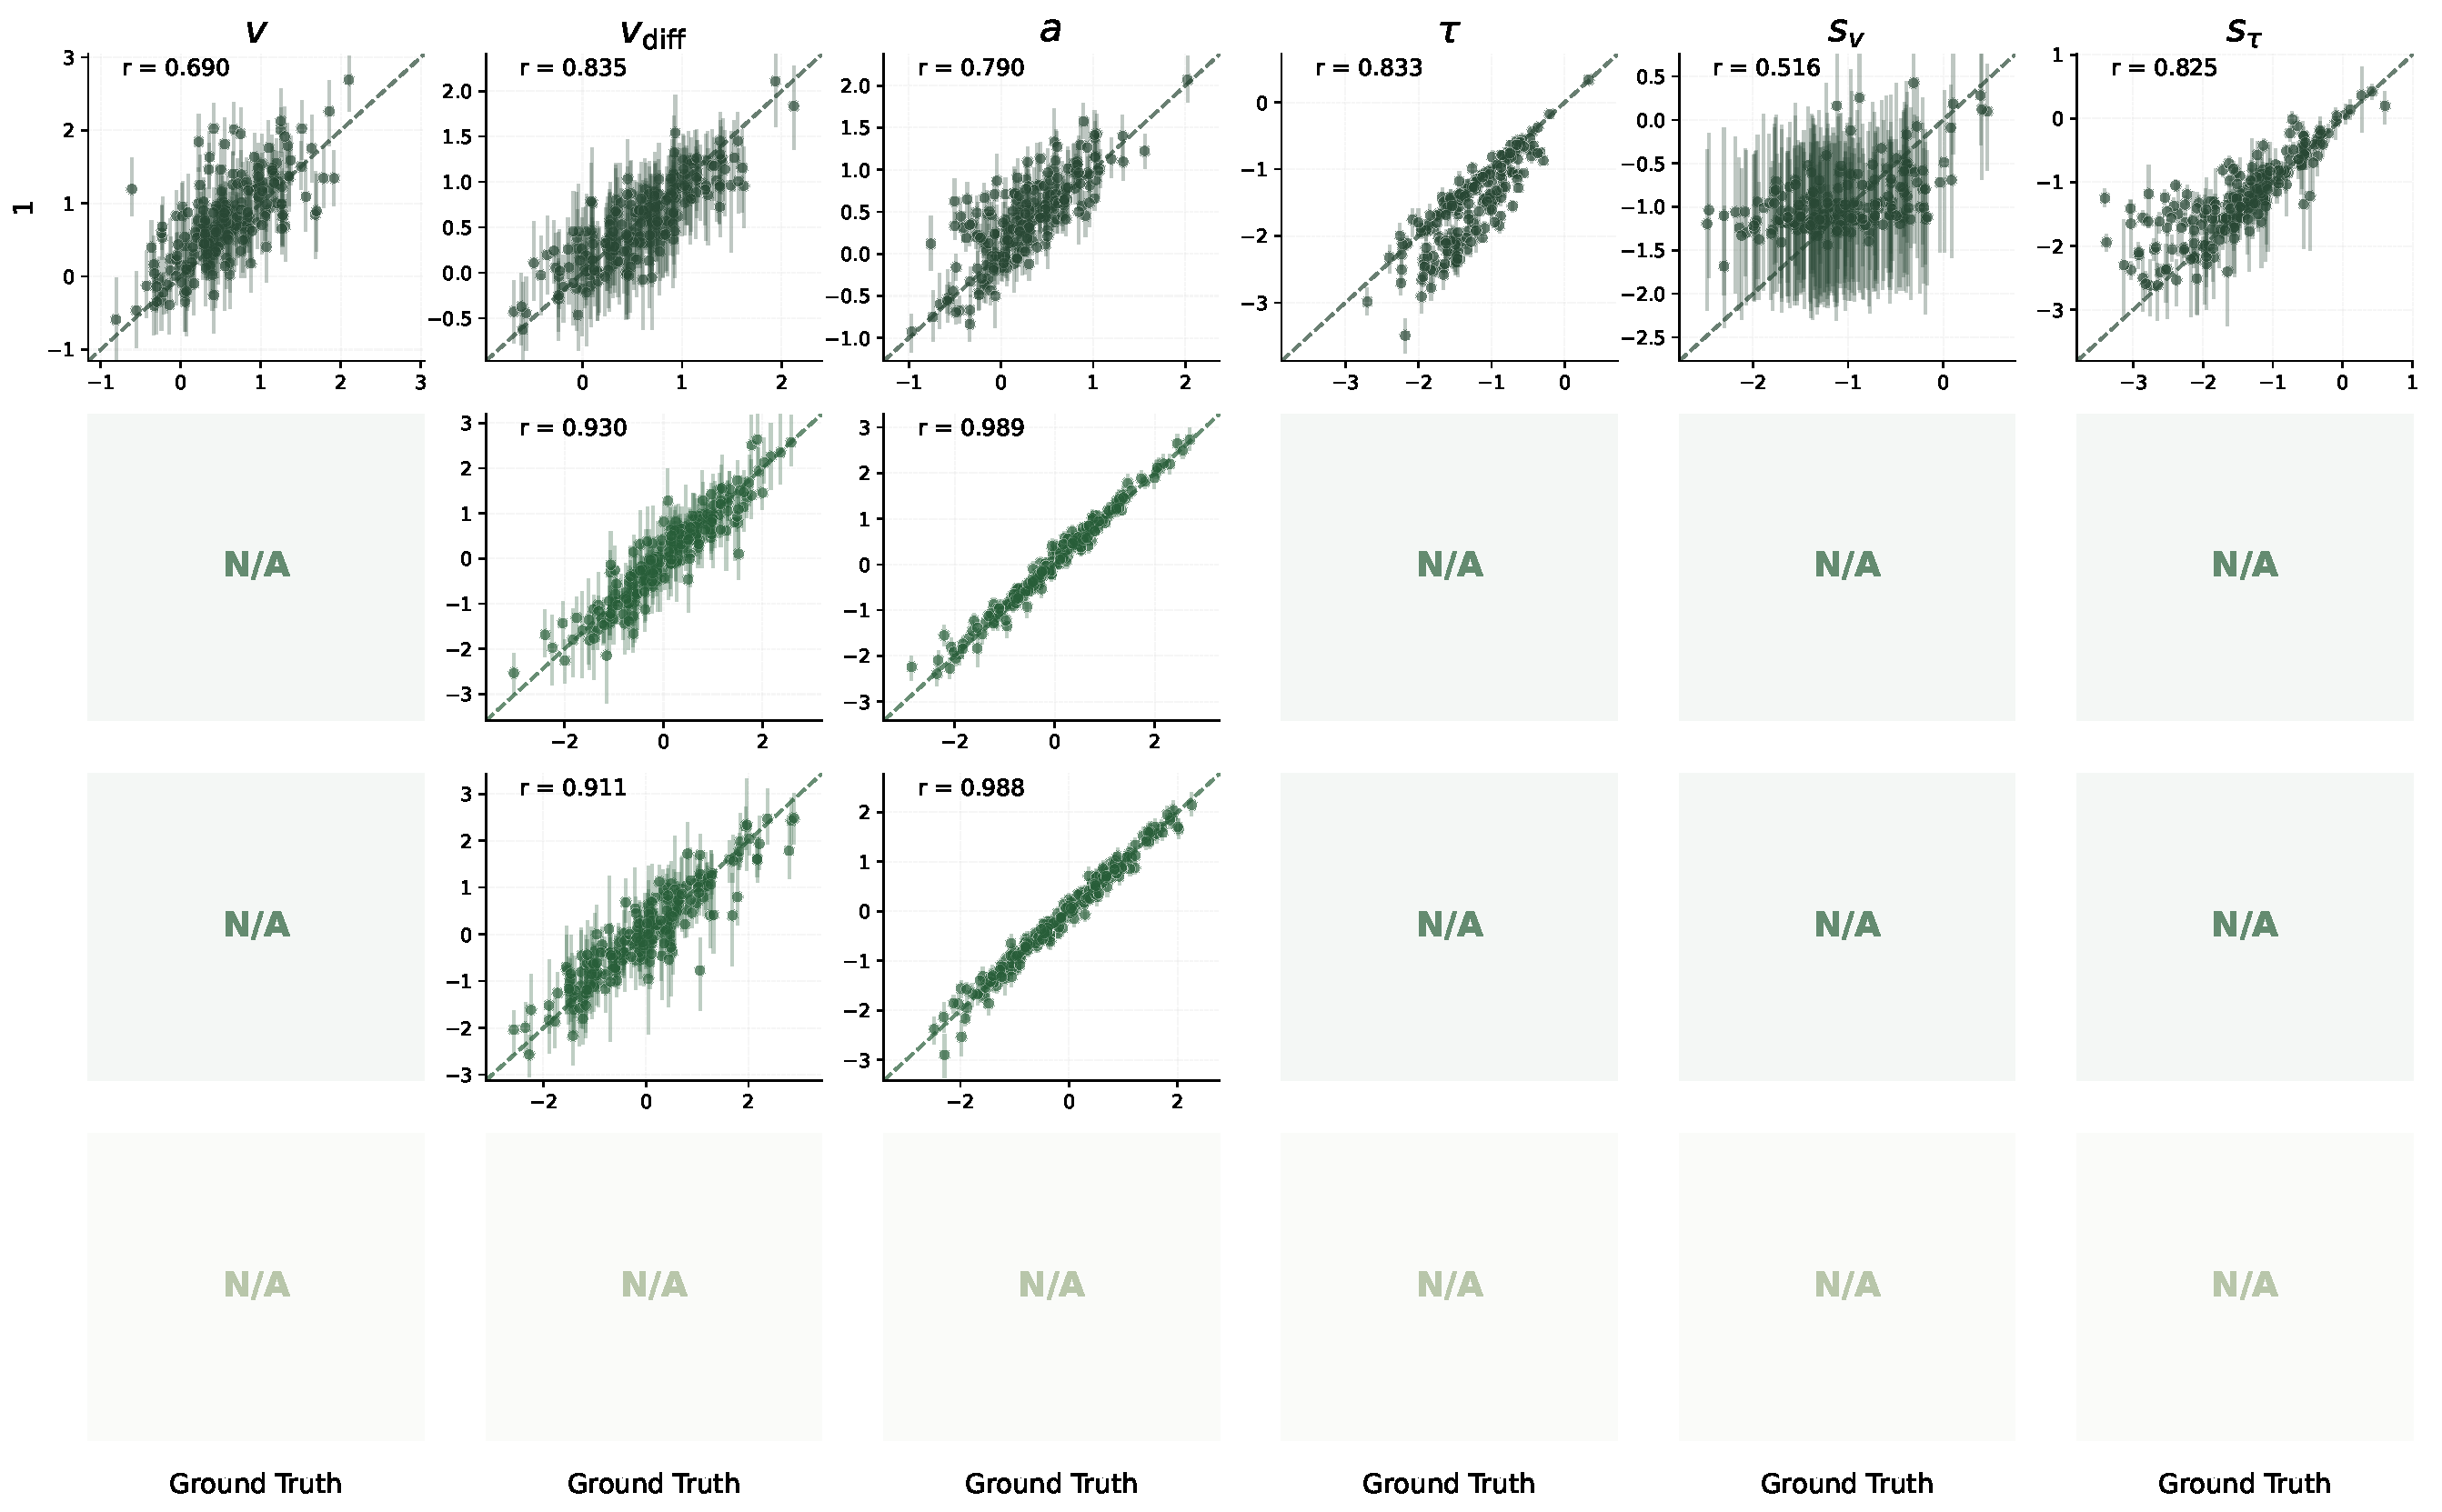
\includegraphics[width=0.99\linewidth]{figures/bf/rdm/regressed/rdm_family_regressed_bf_recovery.pdf}
    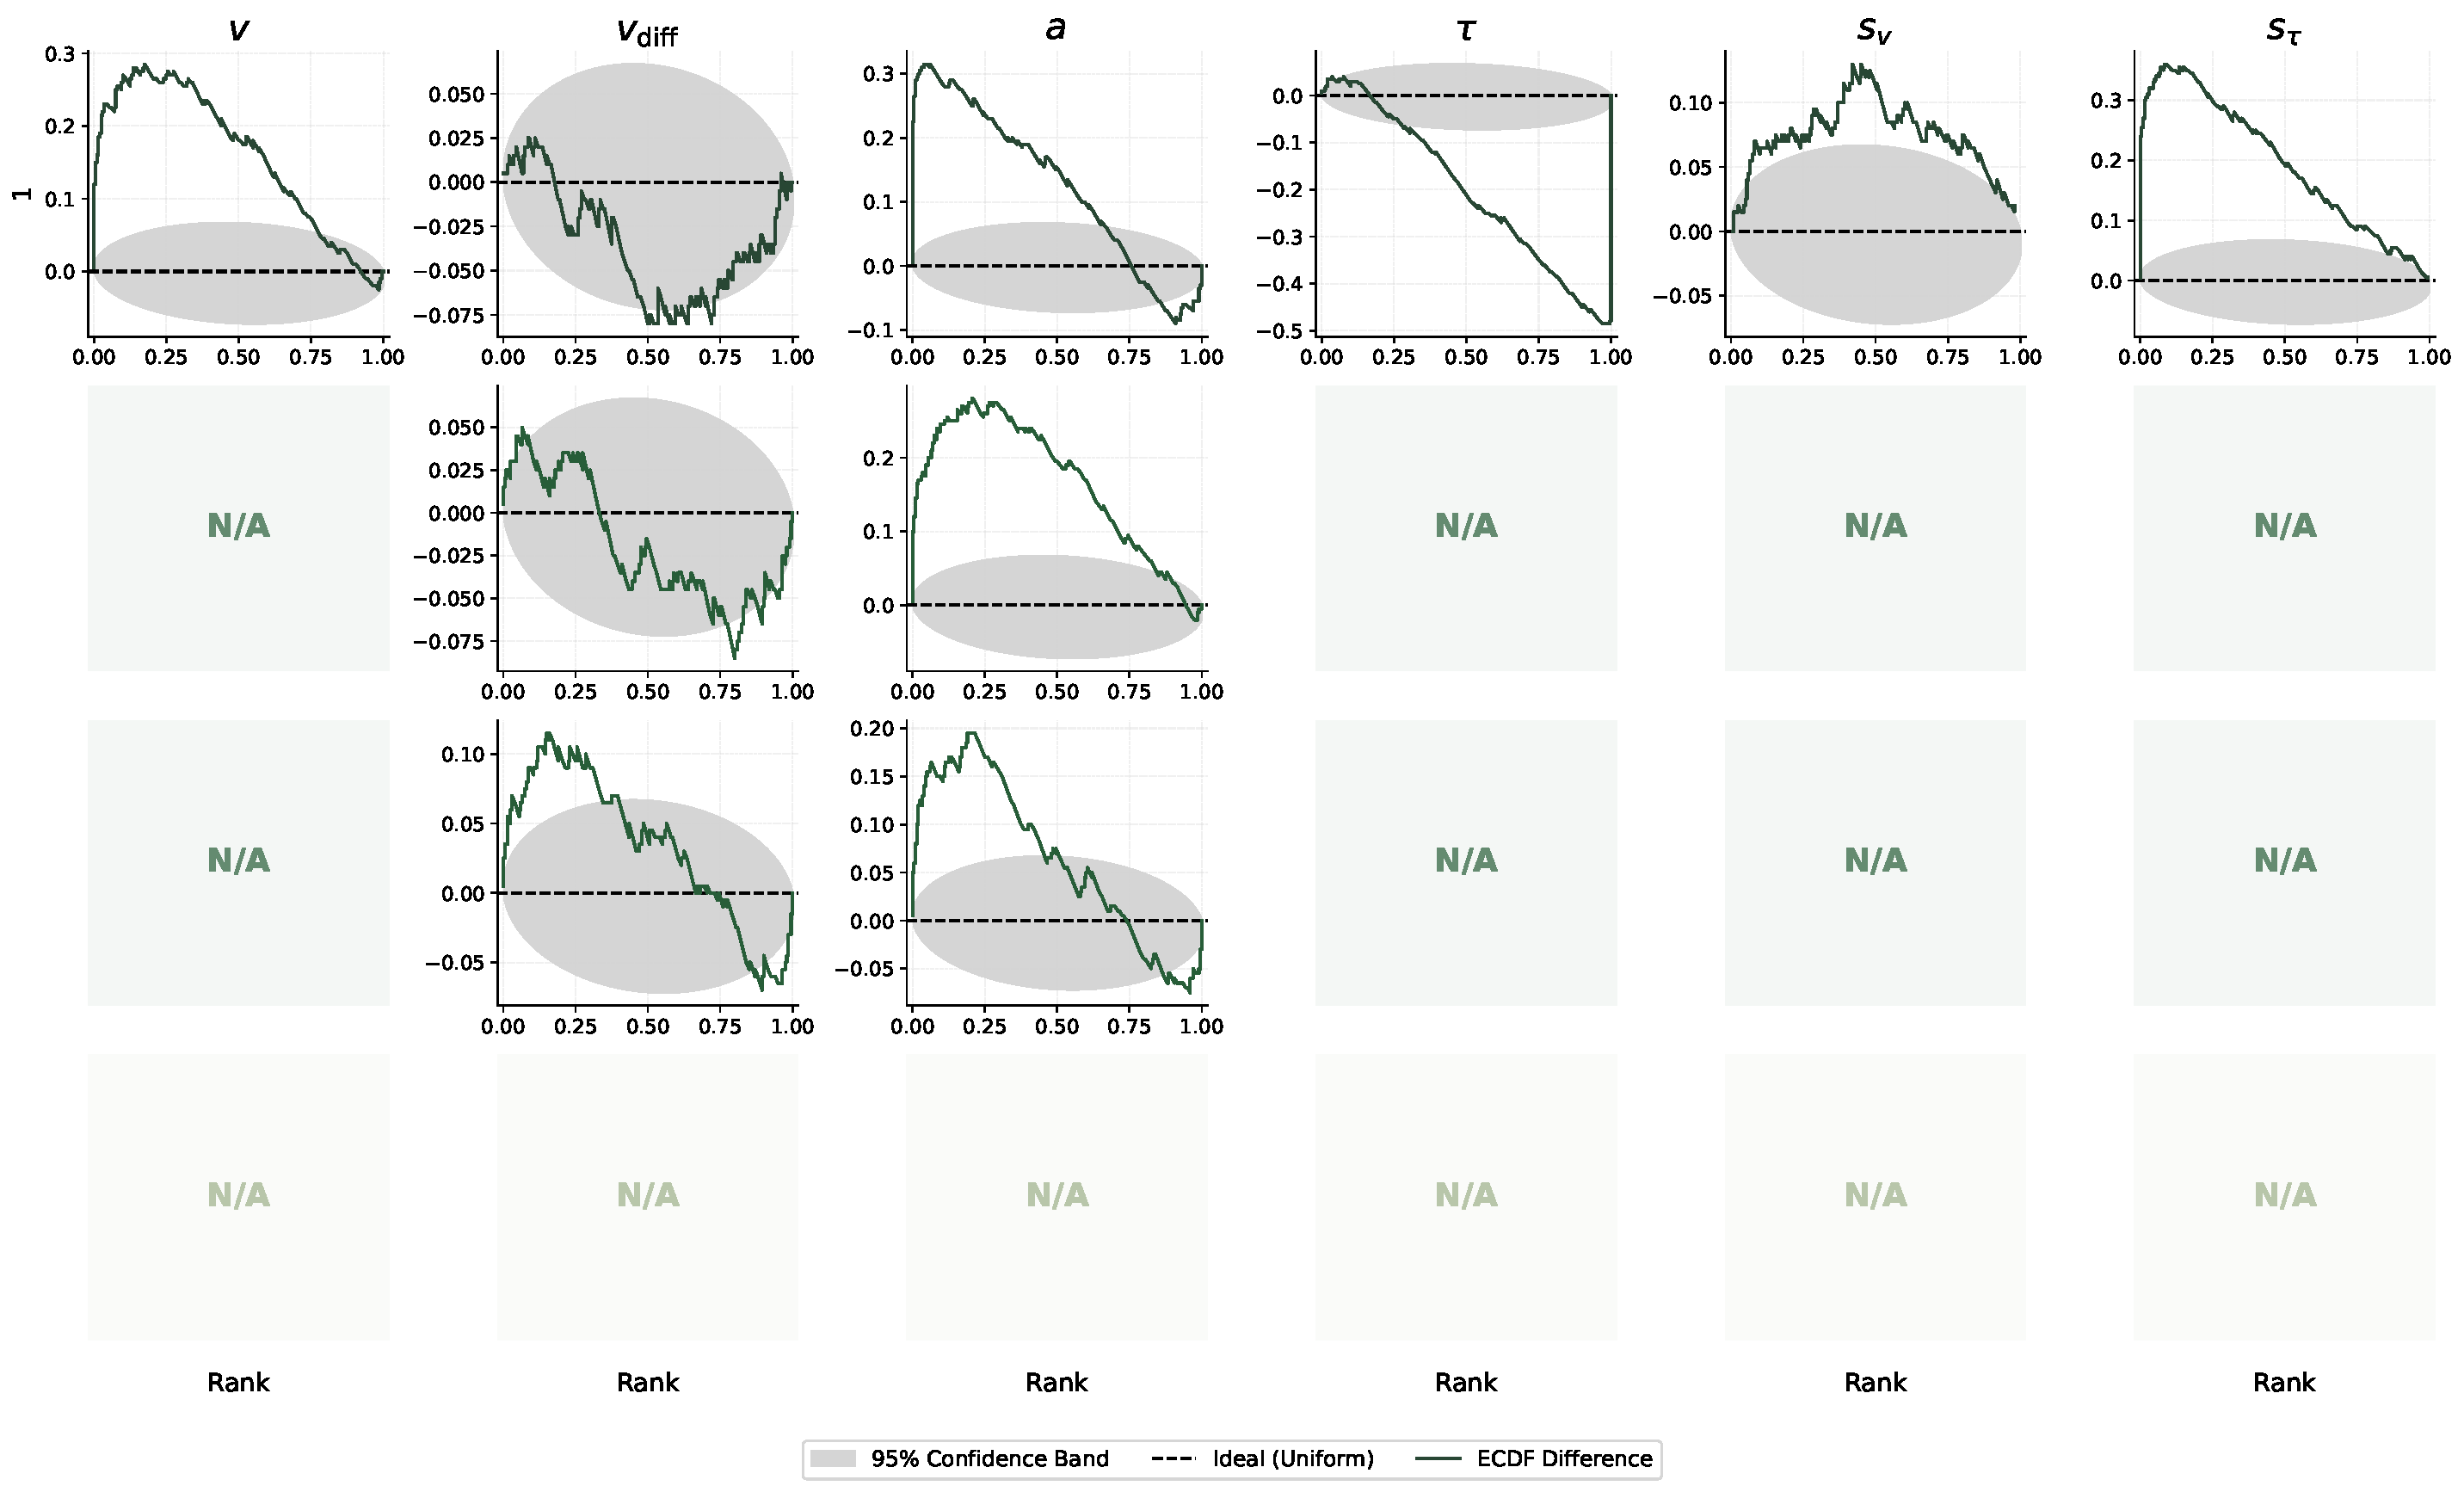
\includegraphics[width=0.99\linewidth]{figures/bf/rdm/regressed/rdm_family_regressed_bf_ecdf.pdf}
    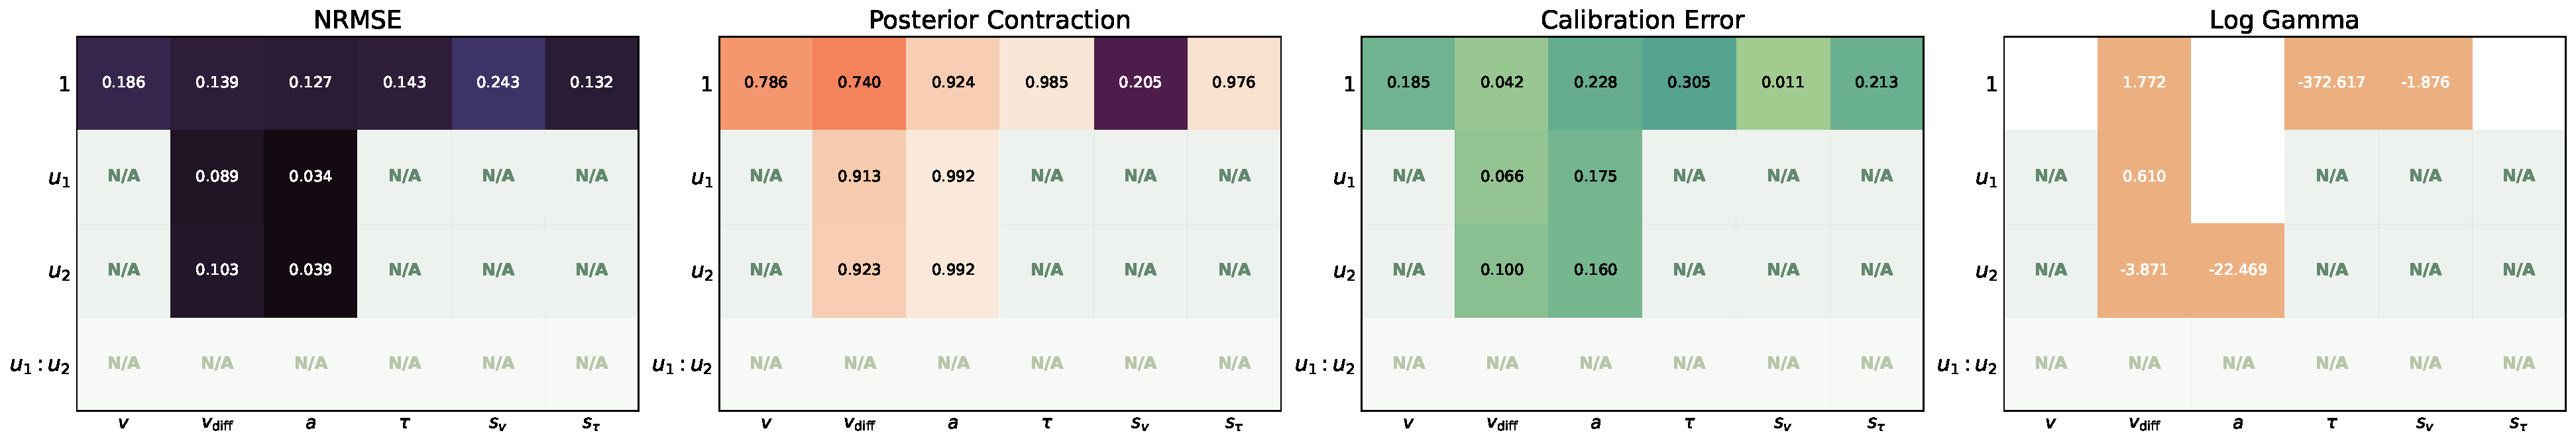
\includegraphics[width=0.99\linewidth]{figures/bf/rdm/regressed/rdm_family_regressed_bf_metrics.pdf}
    \caption{Parameter recovery (\emph{top}), calibration ECDF (\emph{middle}), and parameter-wise metrics (NRMSE, calibration error, and posterior contraction) for RDM baseline (Case \textbf{regressed}).}
    \label{fig:rdm-bf-regressed}
\end{figure}

\begin{figure}
    \centering
    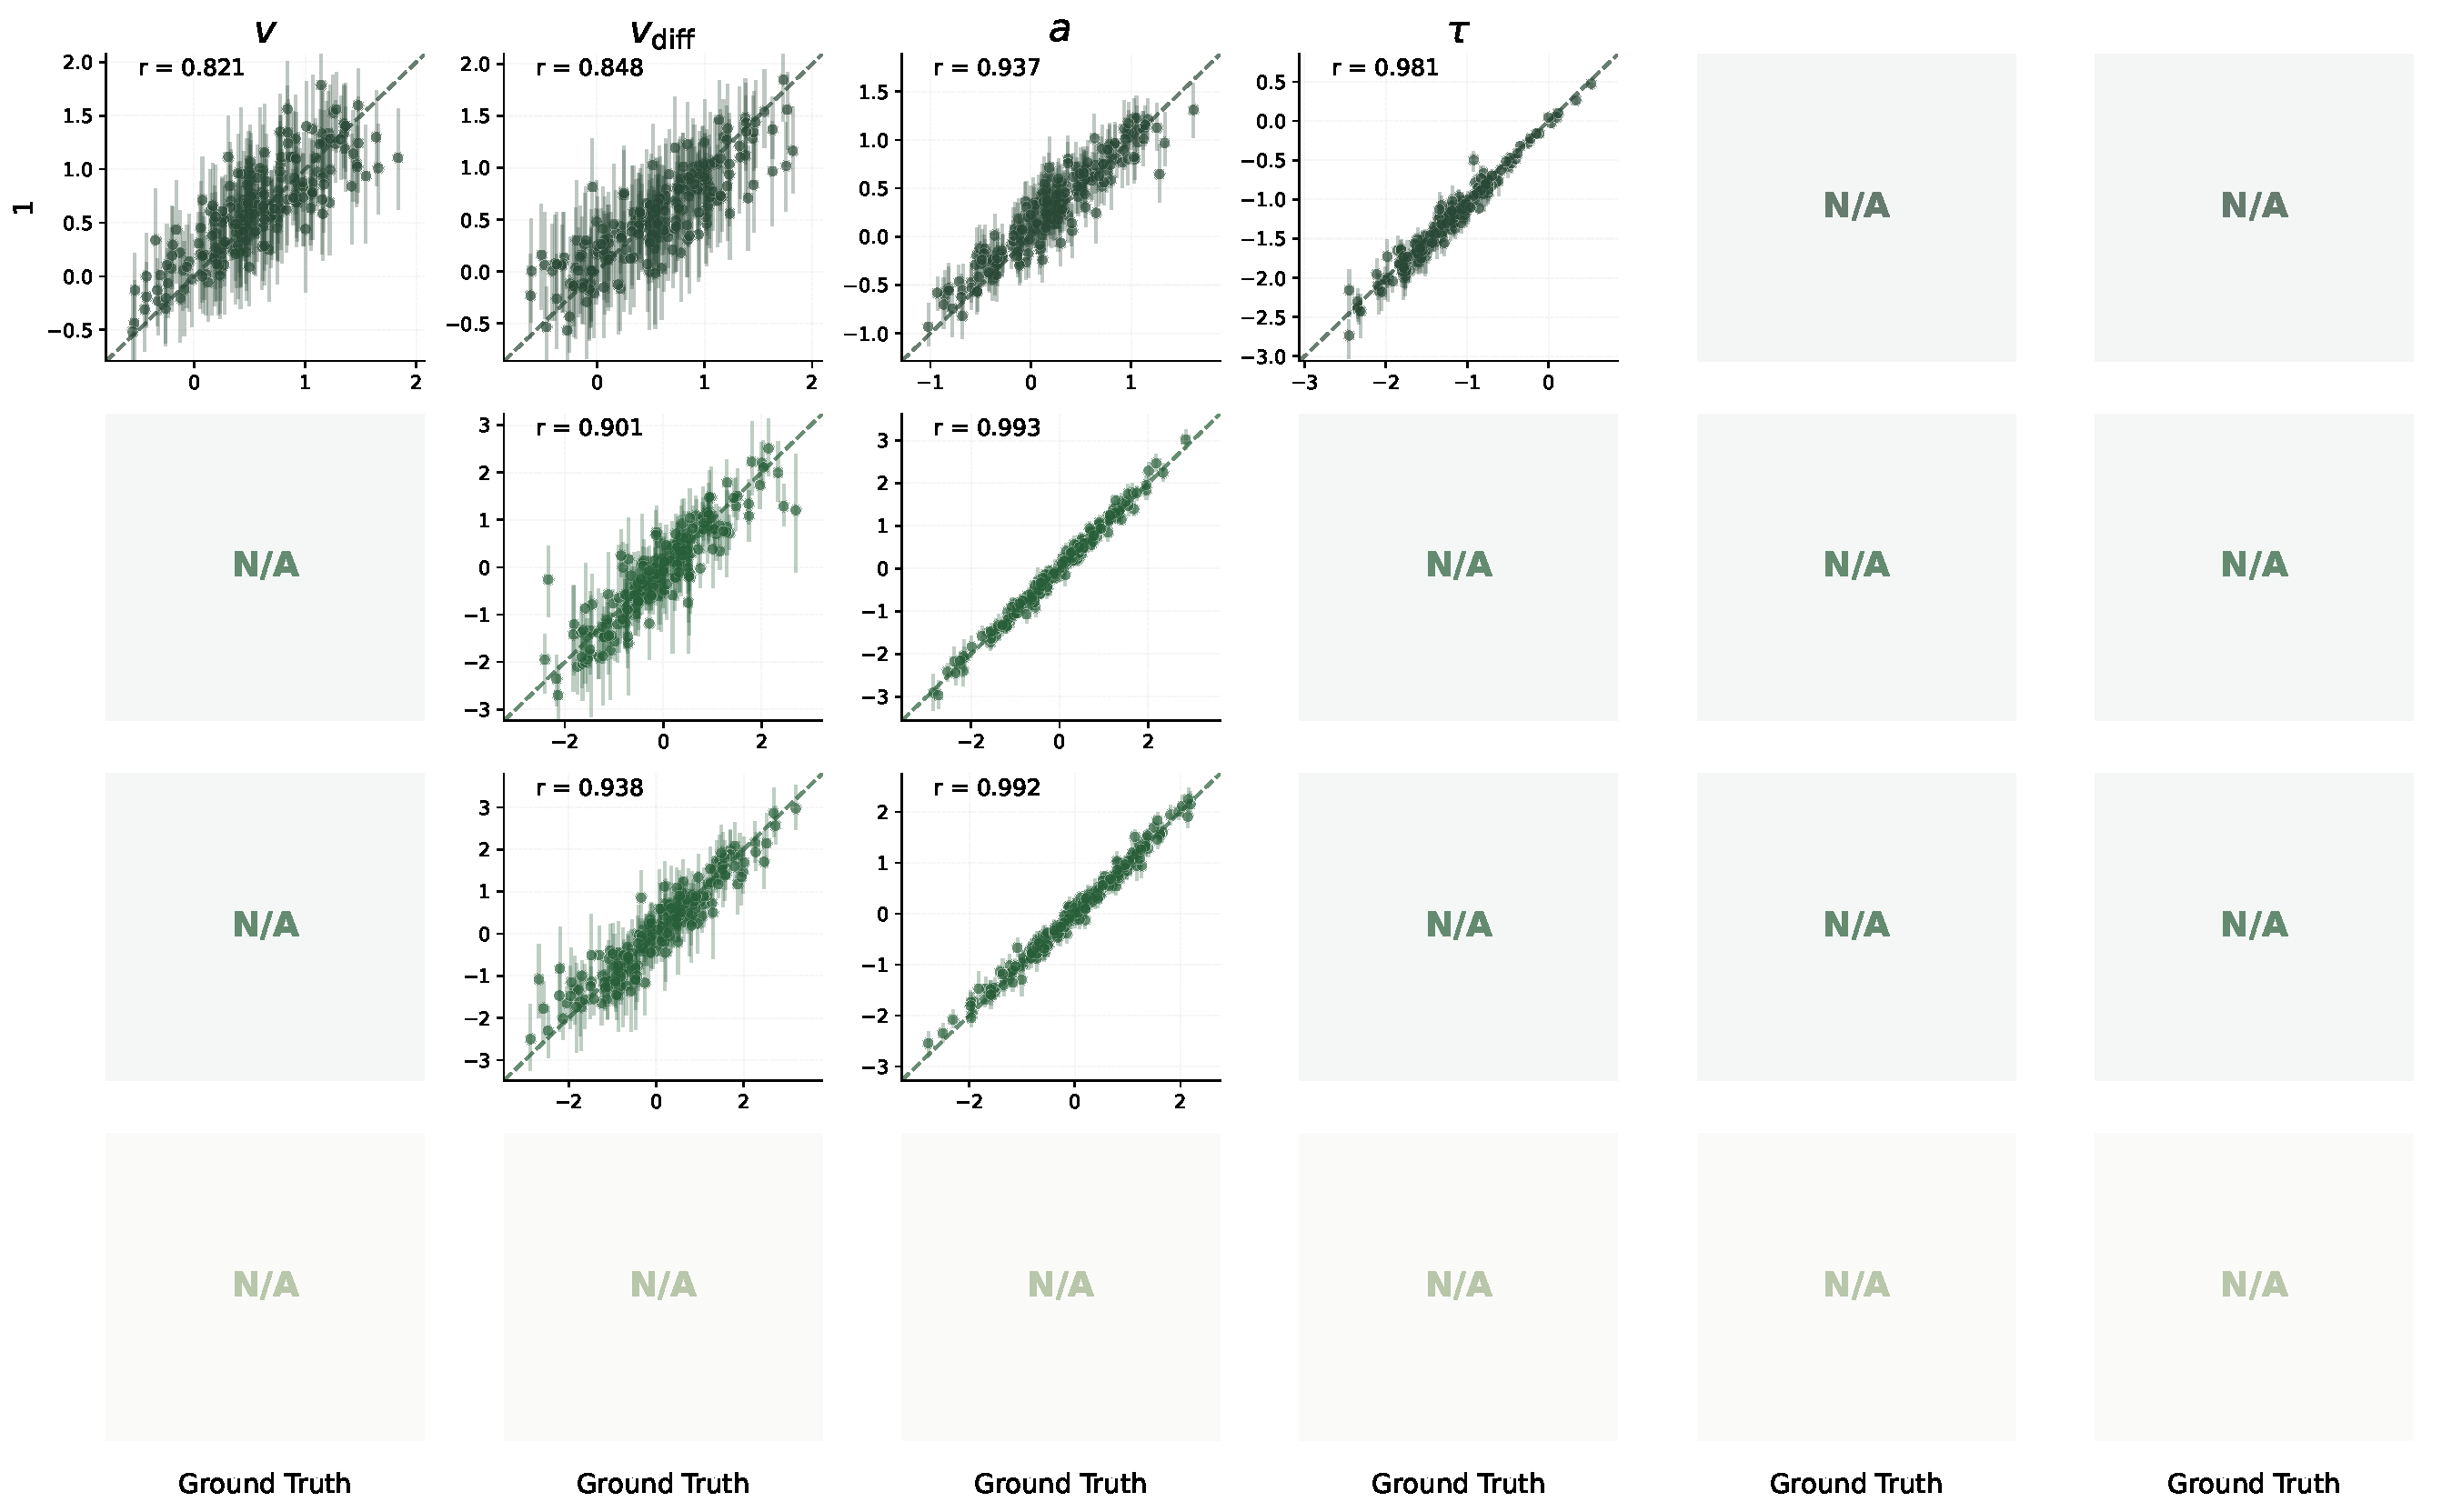
\includegraphics[width=0.99\linewidth]{figures/bf/rdm/fixed_regressed/rdm_family_fixed_regressed_bf_recovery.pdf}
    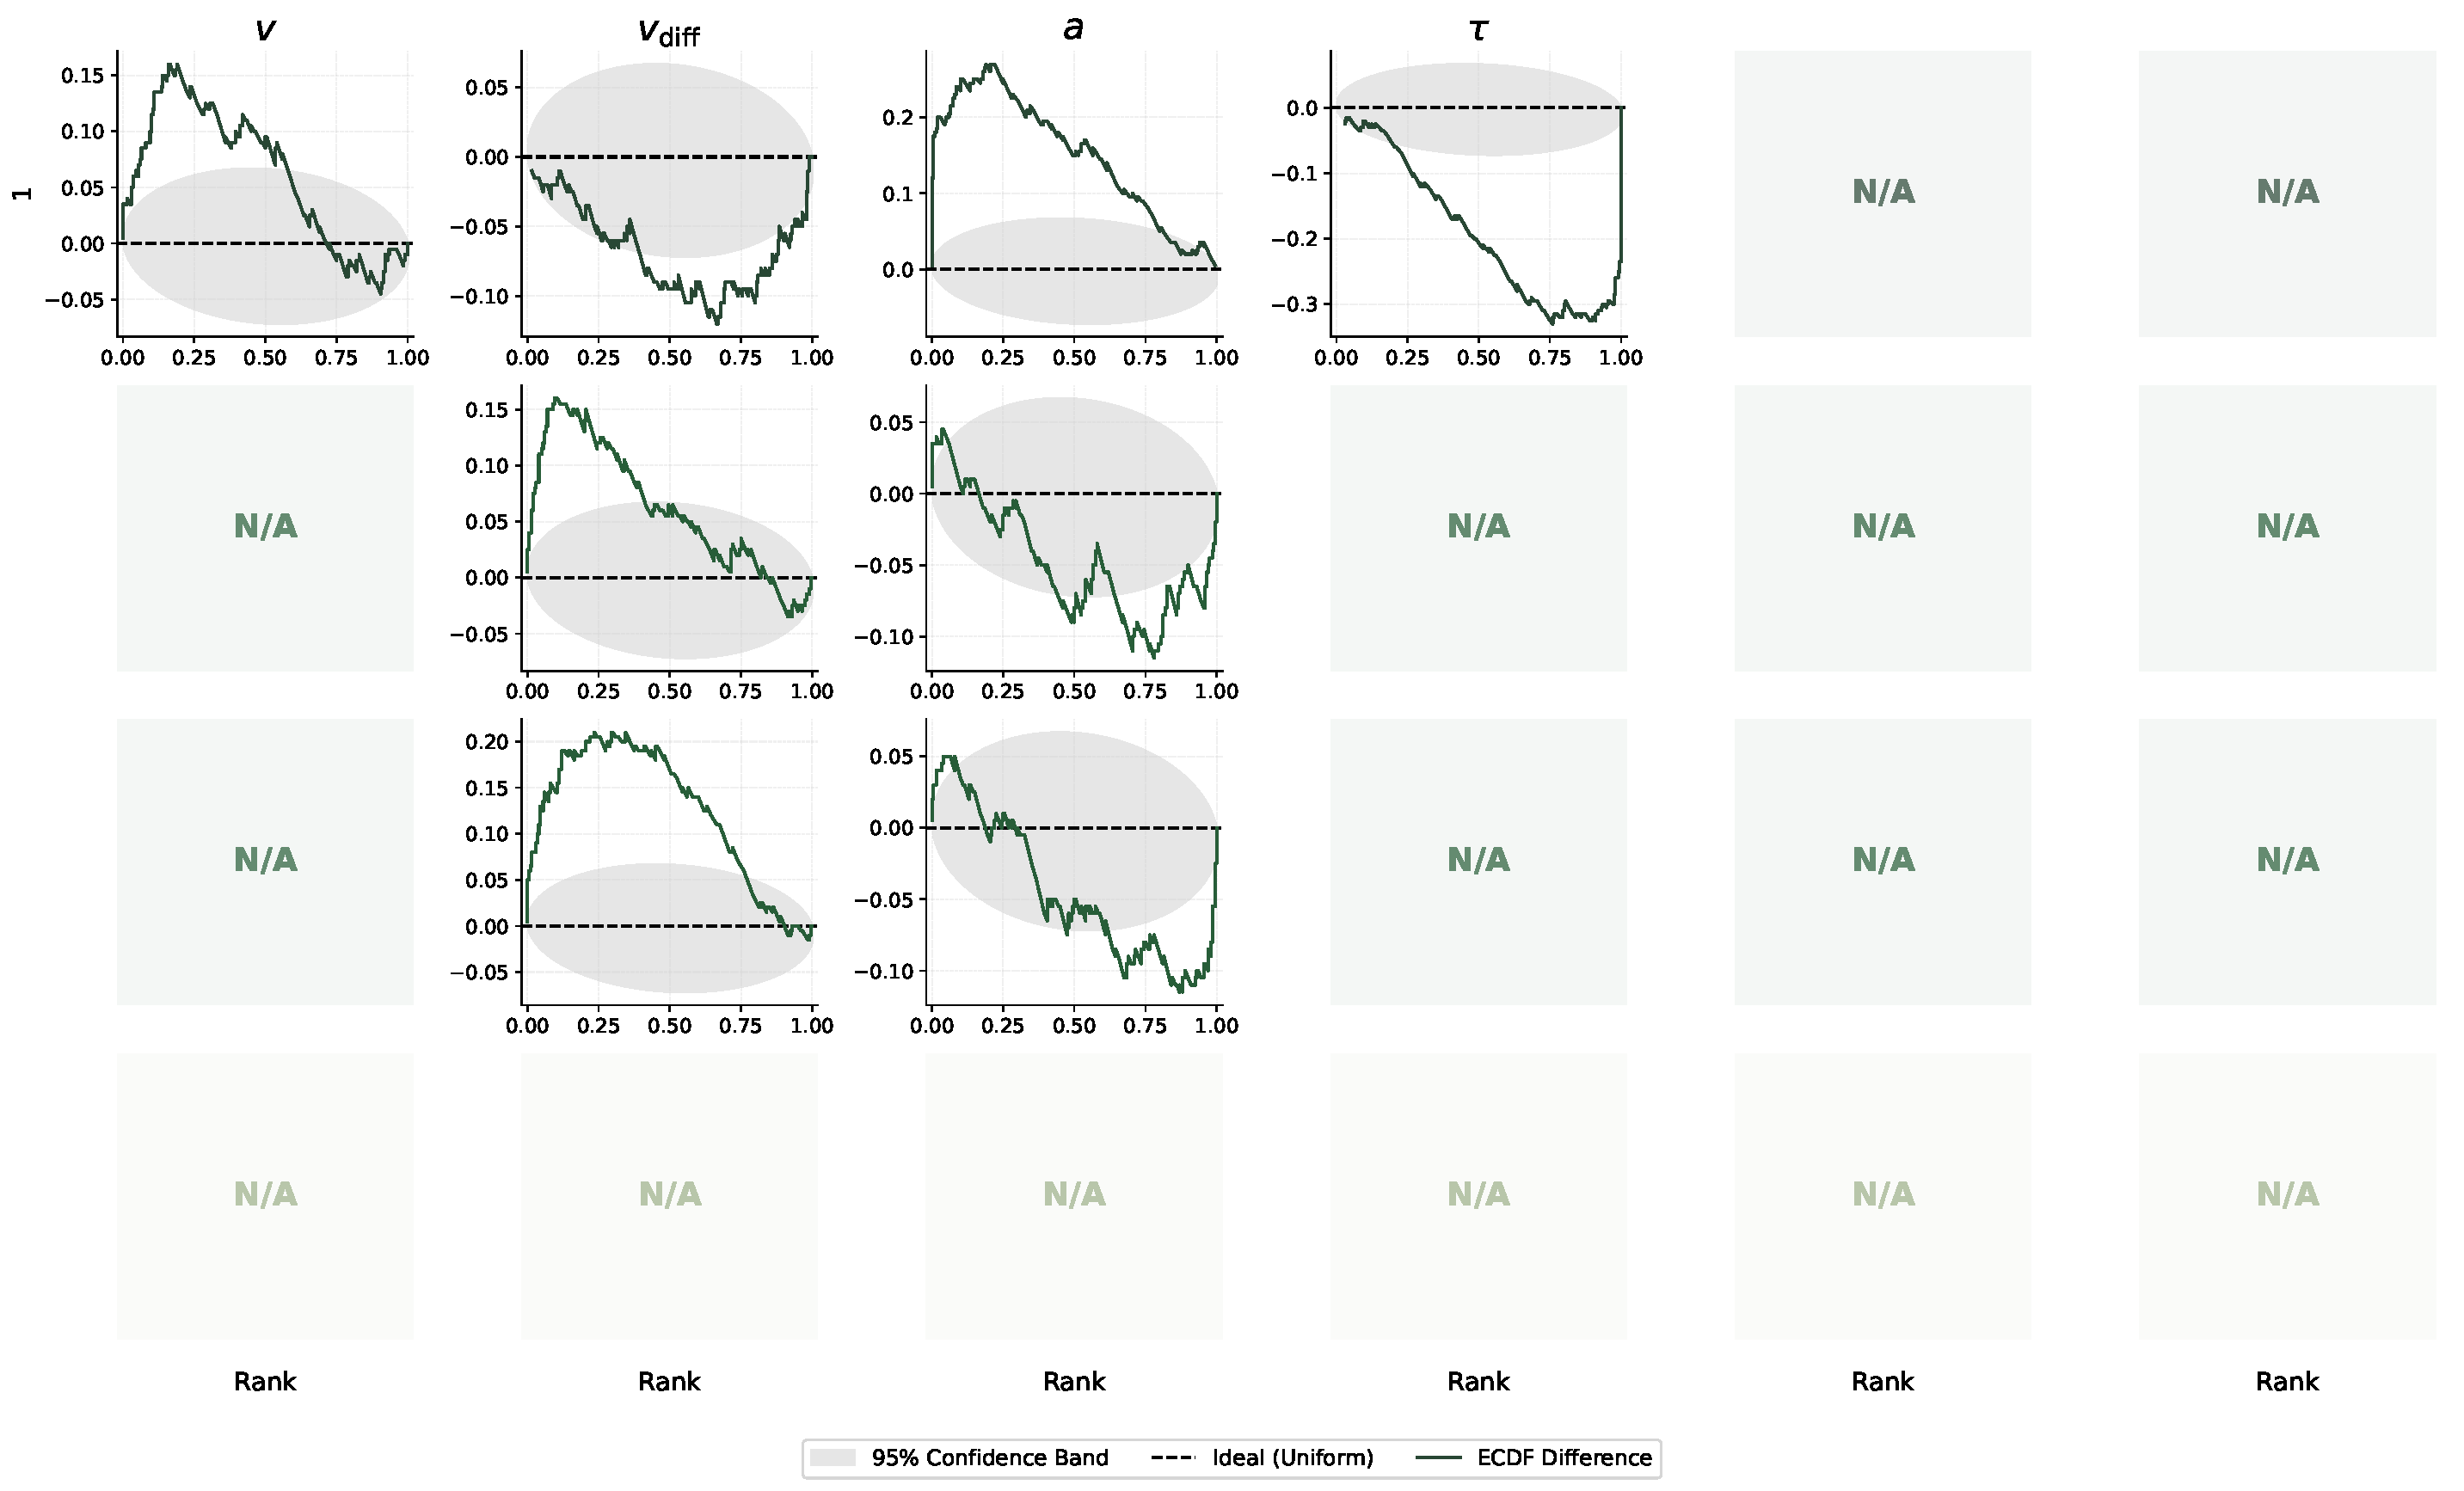
\includegraphics[width=0.99\linewidth]{figures/bf/rdm/fixed_regressed/rdm_family_fixed_regressed_bf_ecdf.pdf}
    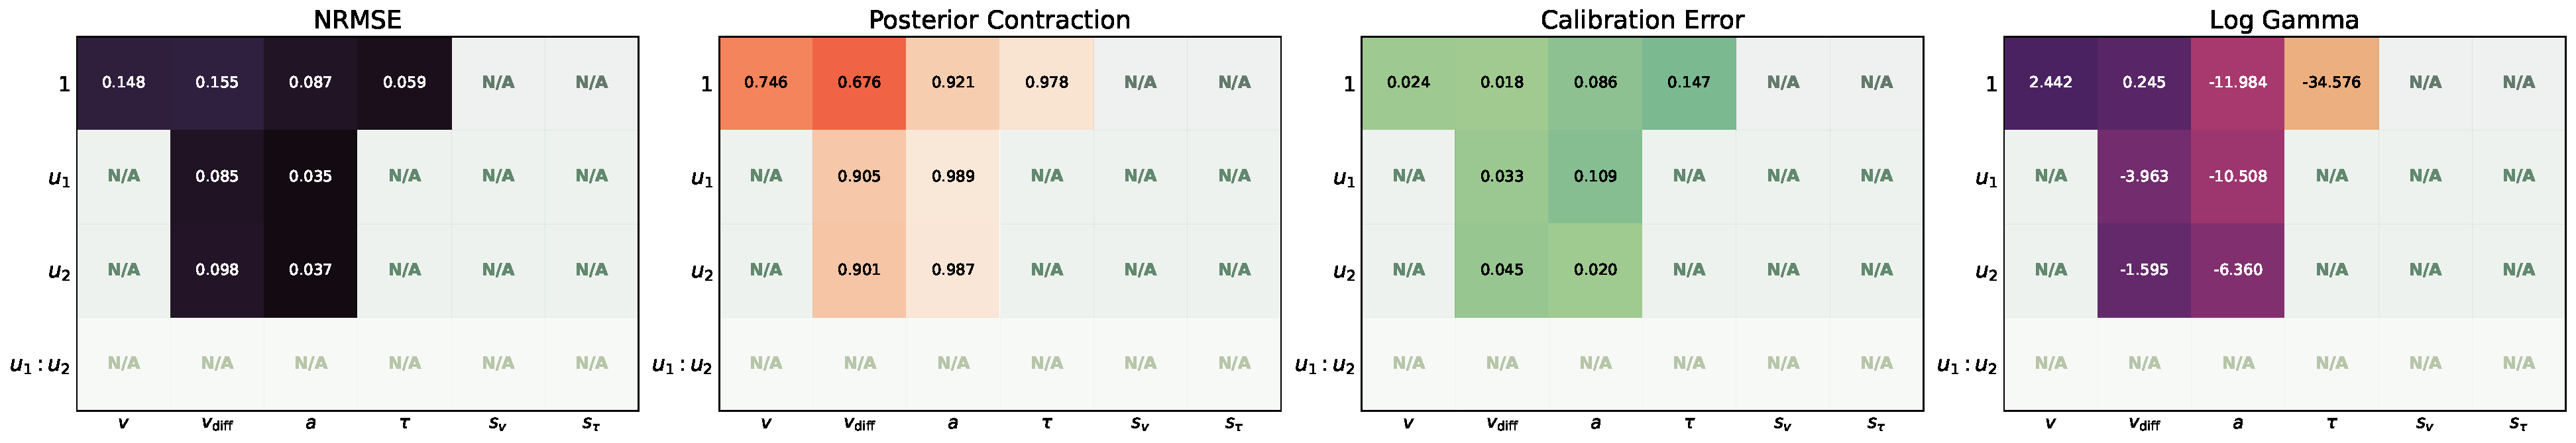
\includegraphics[width=0.99\linewidth]{figures/bf/rdm/fixed_regressed/rdm_family_fixed_regressed_bf_metrics.pdf}
    \caption{Parameter recovery (\emph{top}), calibration ECDF (\emph{middle}), and parameter-wise metrics (NRMSE, calibration error, and posterior contraction) for RDM baseline (Case \textbf{fixed\_regressed}).}
    \label{fig:rdm-bf-fixed-regressed}
\end{figure}

\begin{figure}
    \centering
    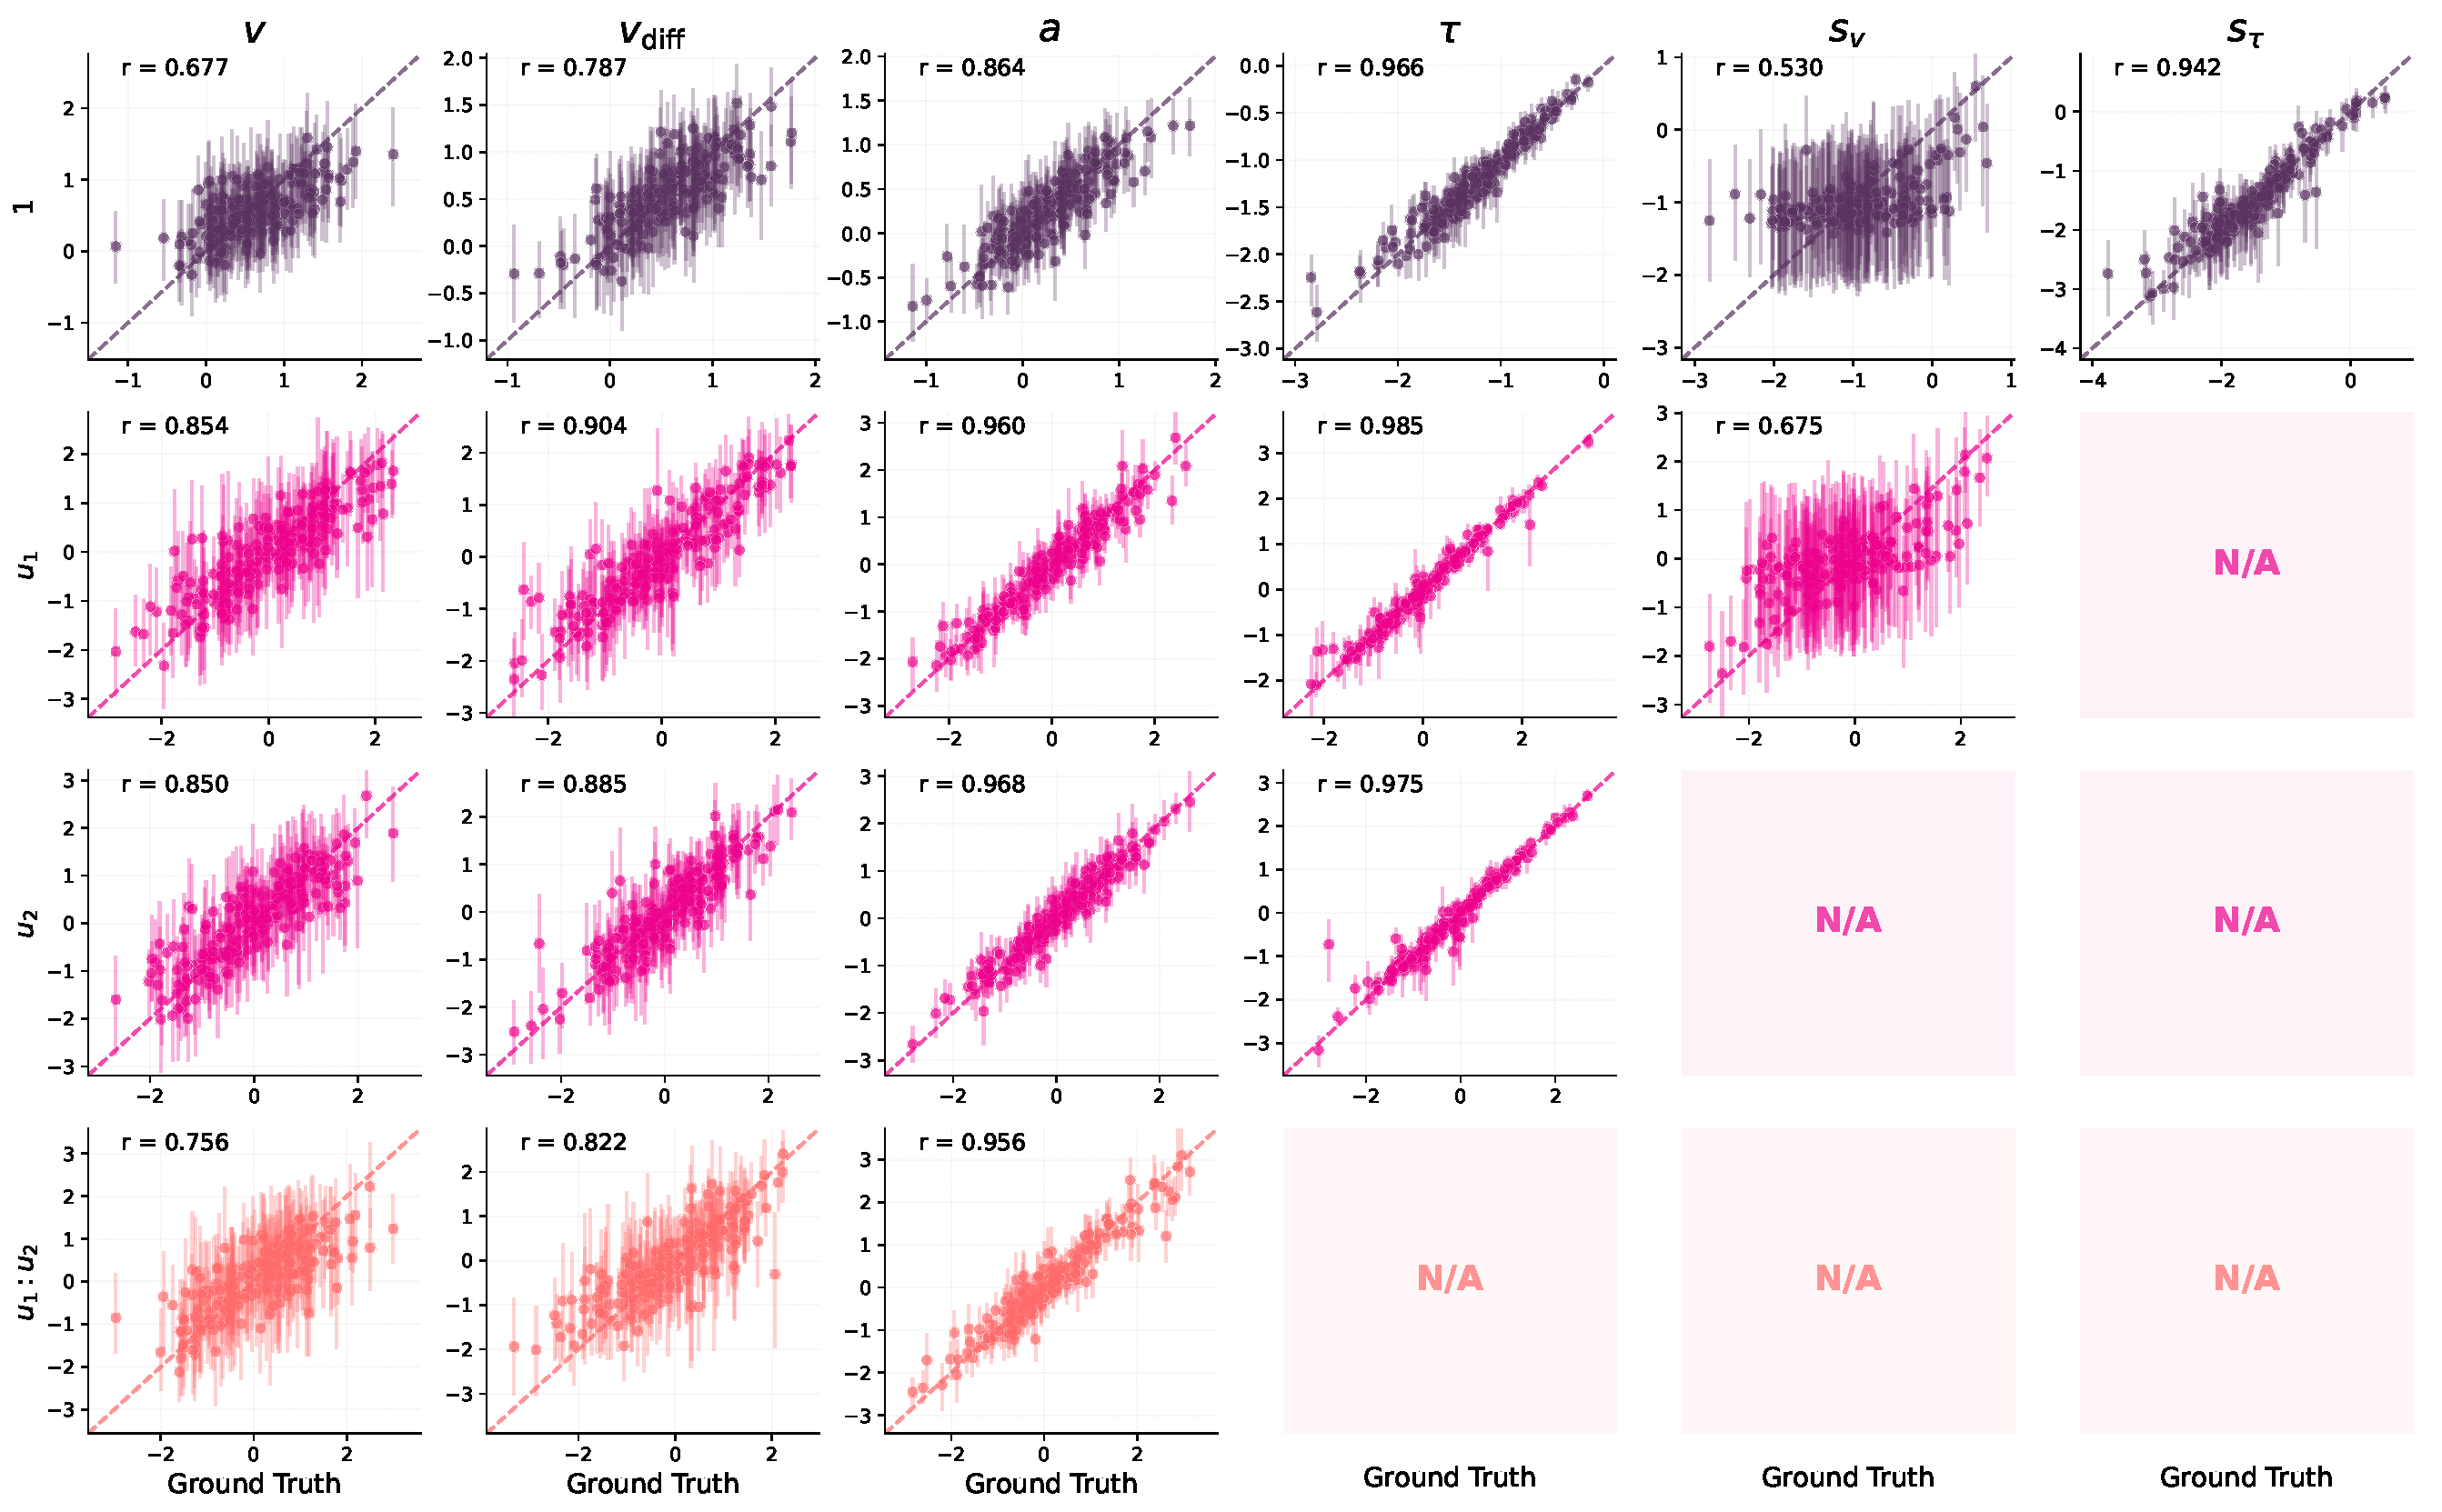
\includegraphics[width=0.99\linewidth]{figures/bf/rdm/interaction/rdm_family_interaction_bf_recovery.pdf}
    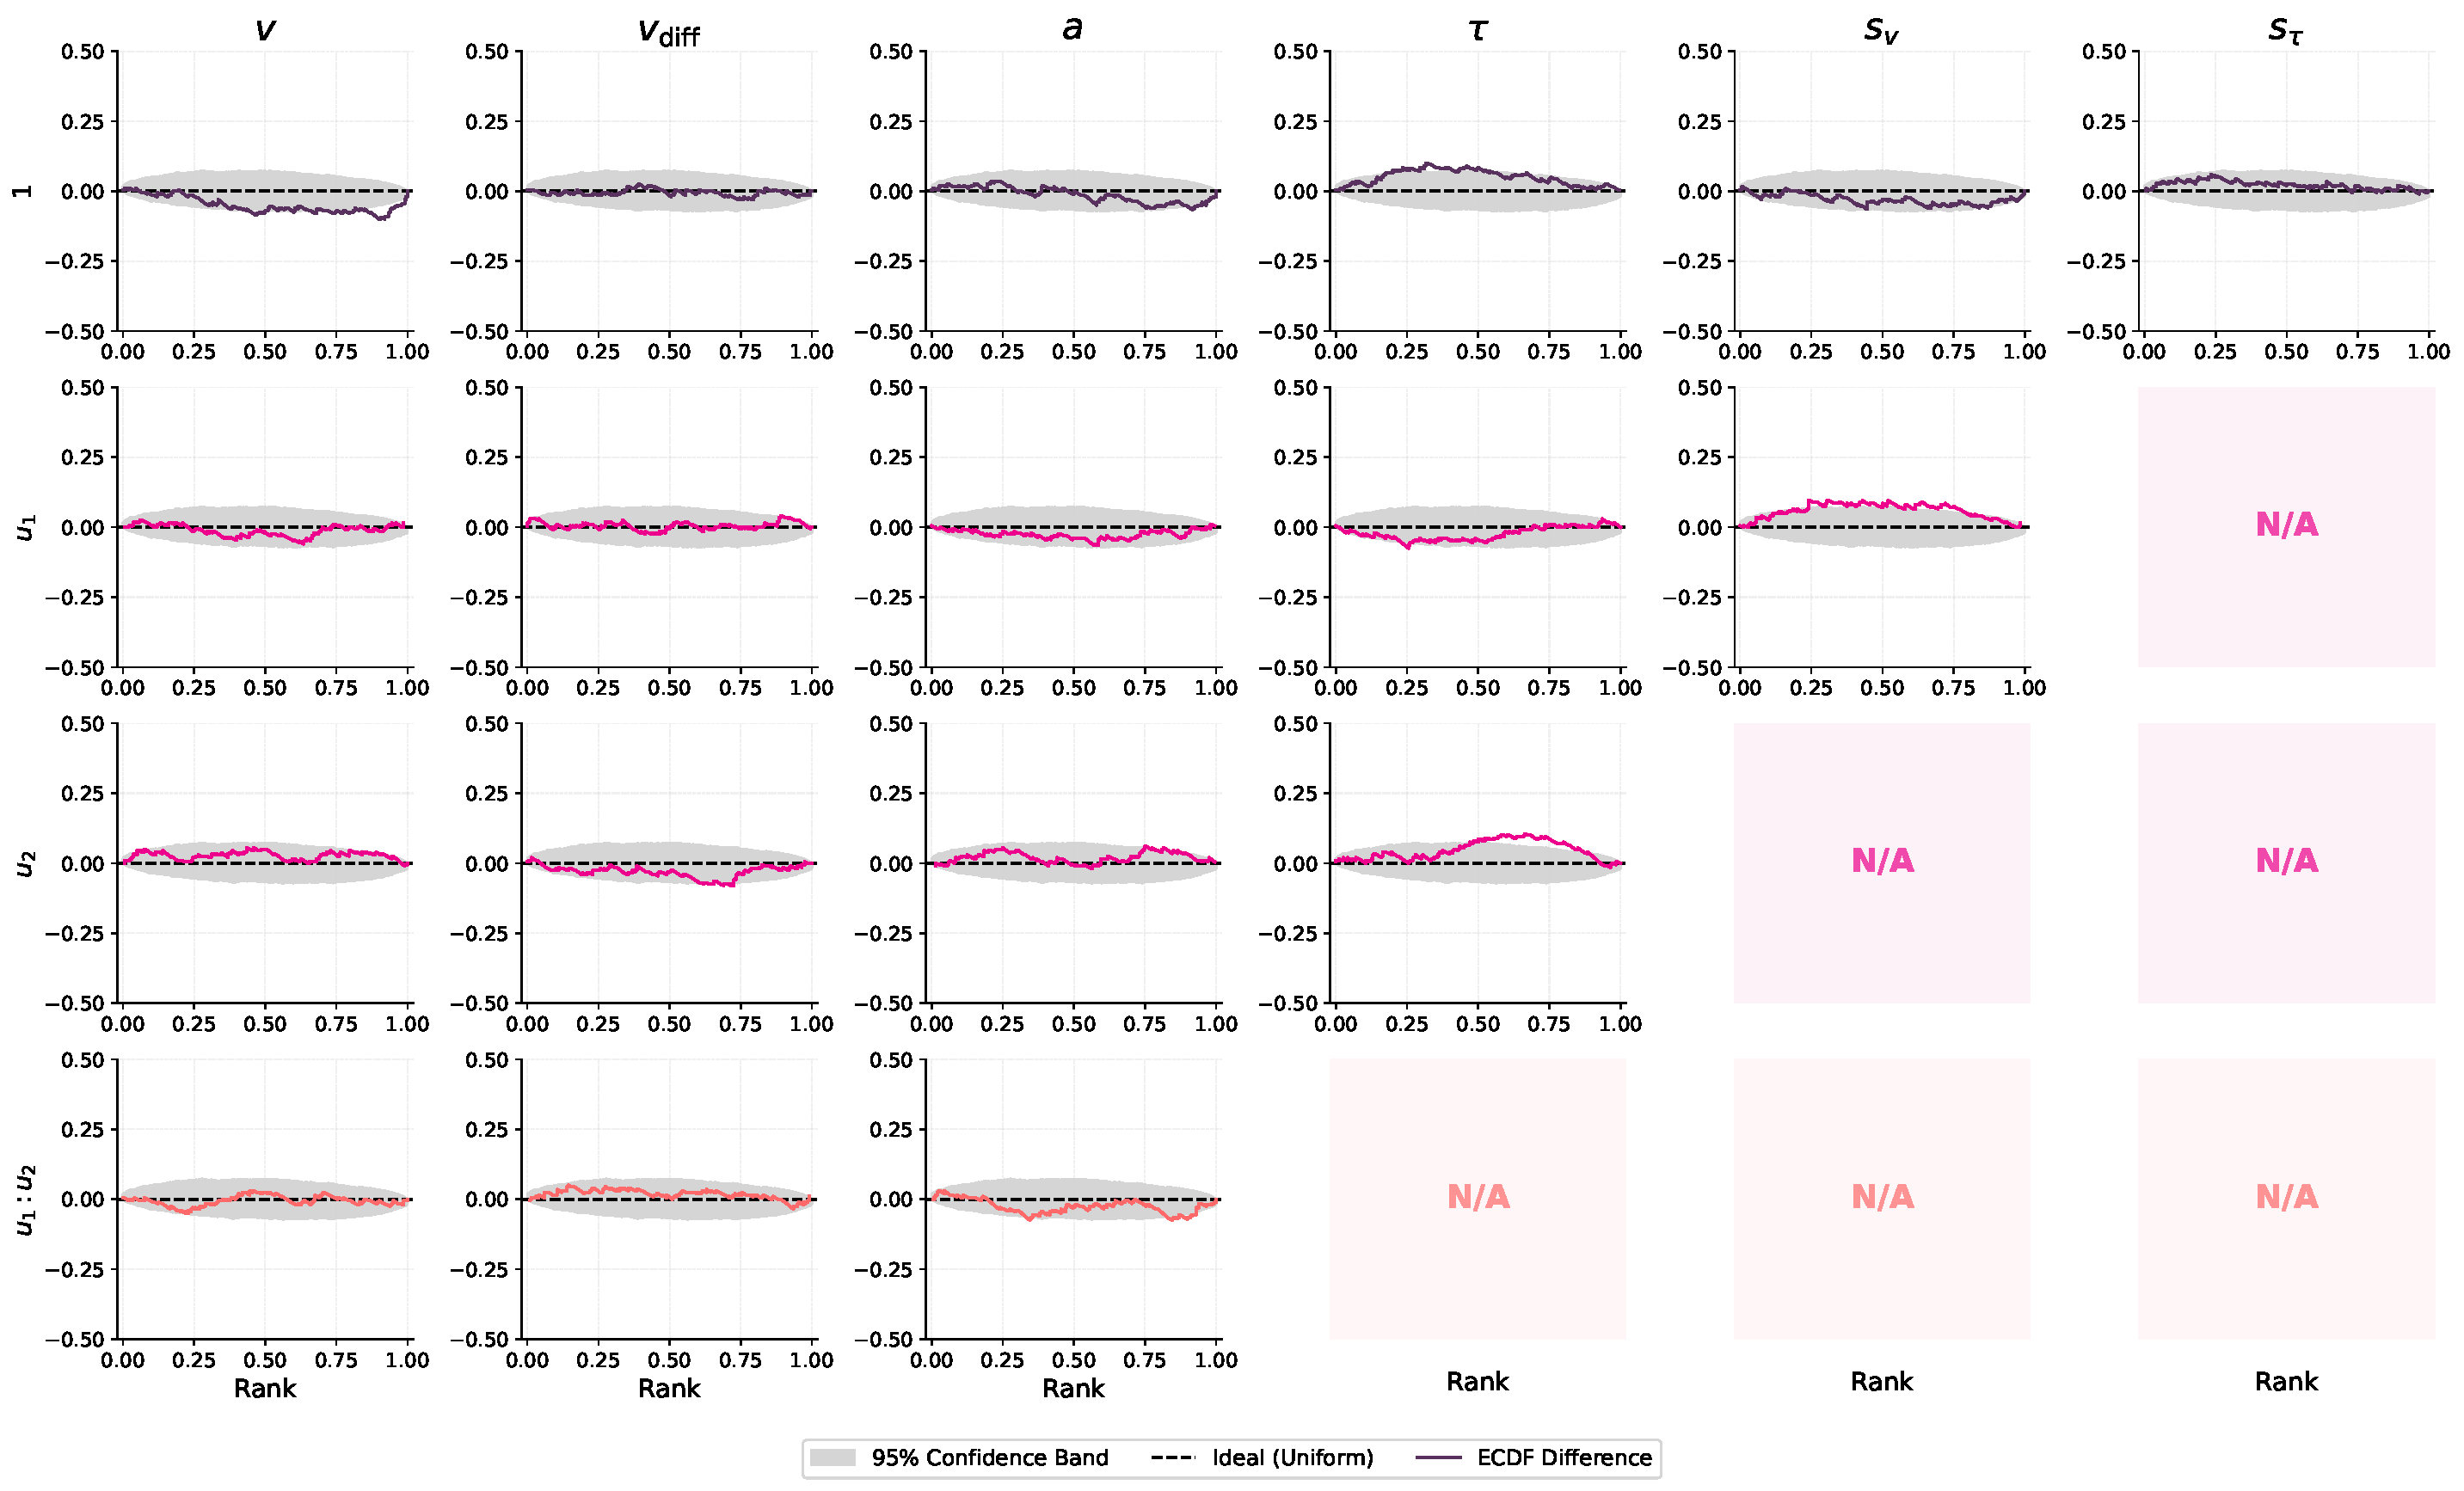
\includegraphics[width=0.99\linewidth]{figures/bf/rdm/interaction/rdm_family_interaction_bf_ecdf.pdf}
    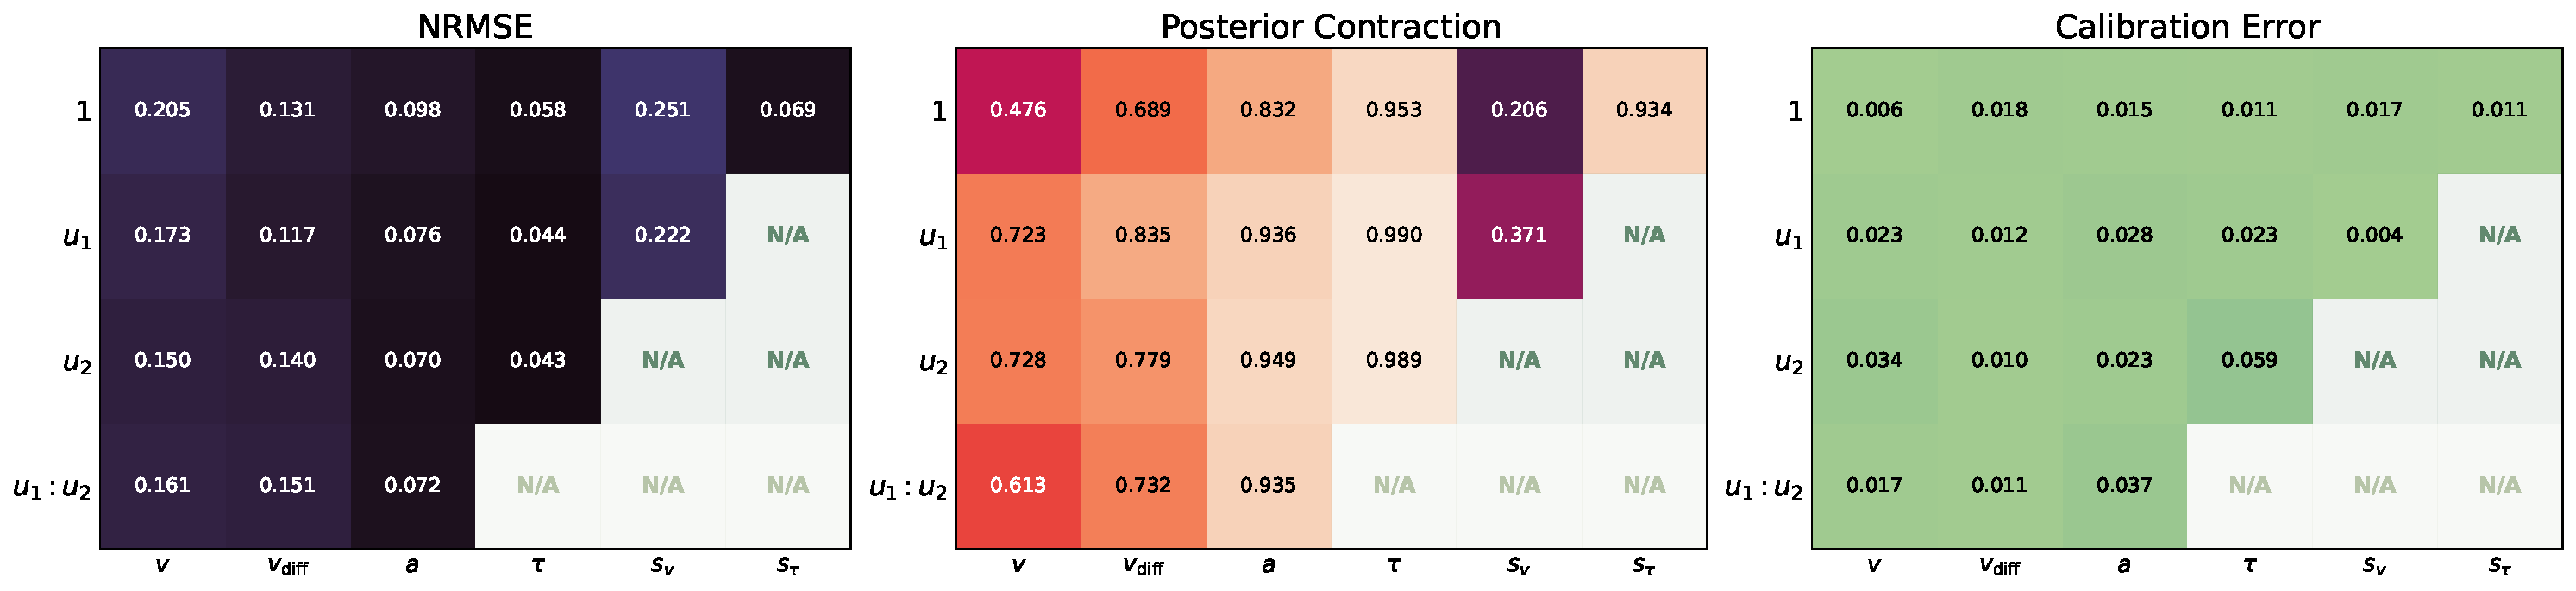
\includegraphics[width=0.99\linewidth]{figures/bf/rdm/interaction/rdm_family_interaction_bf_metrics.pdf}
    \caption{Parameter recovery (\emph{top}), calibration ECDF (\emph{middle}), and parameter-wise metrics (NRMSE, calibration error, and posterior contraction) for RDM baseline (Case \textbf{interaction}).}
    \label{fig:rdm-bf-interaction}
\end{figure}

% ========================================
% RDM MODEL FAMILY (fm)
% ========================================

\begin{figure}
    \centering
    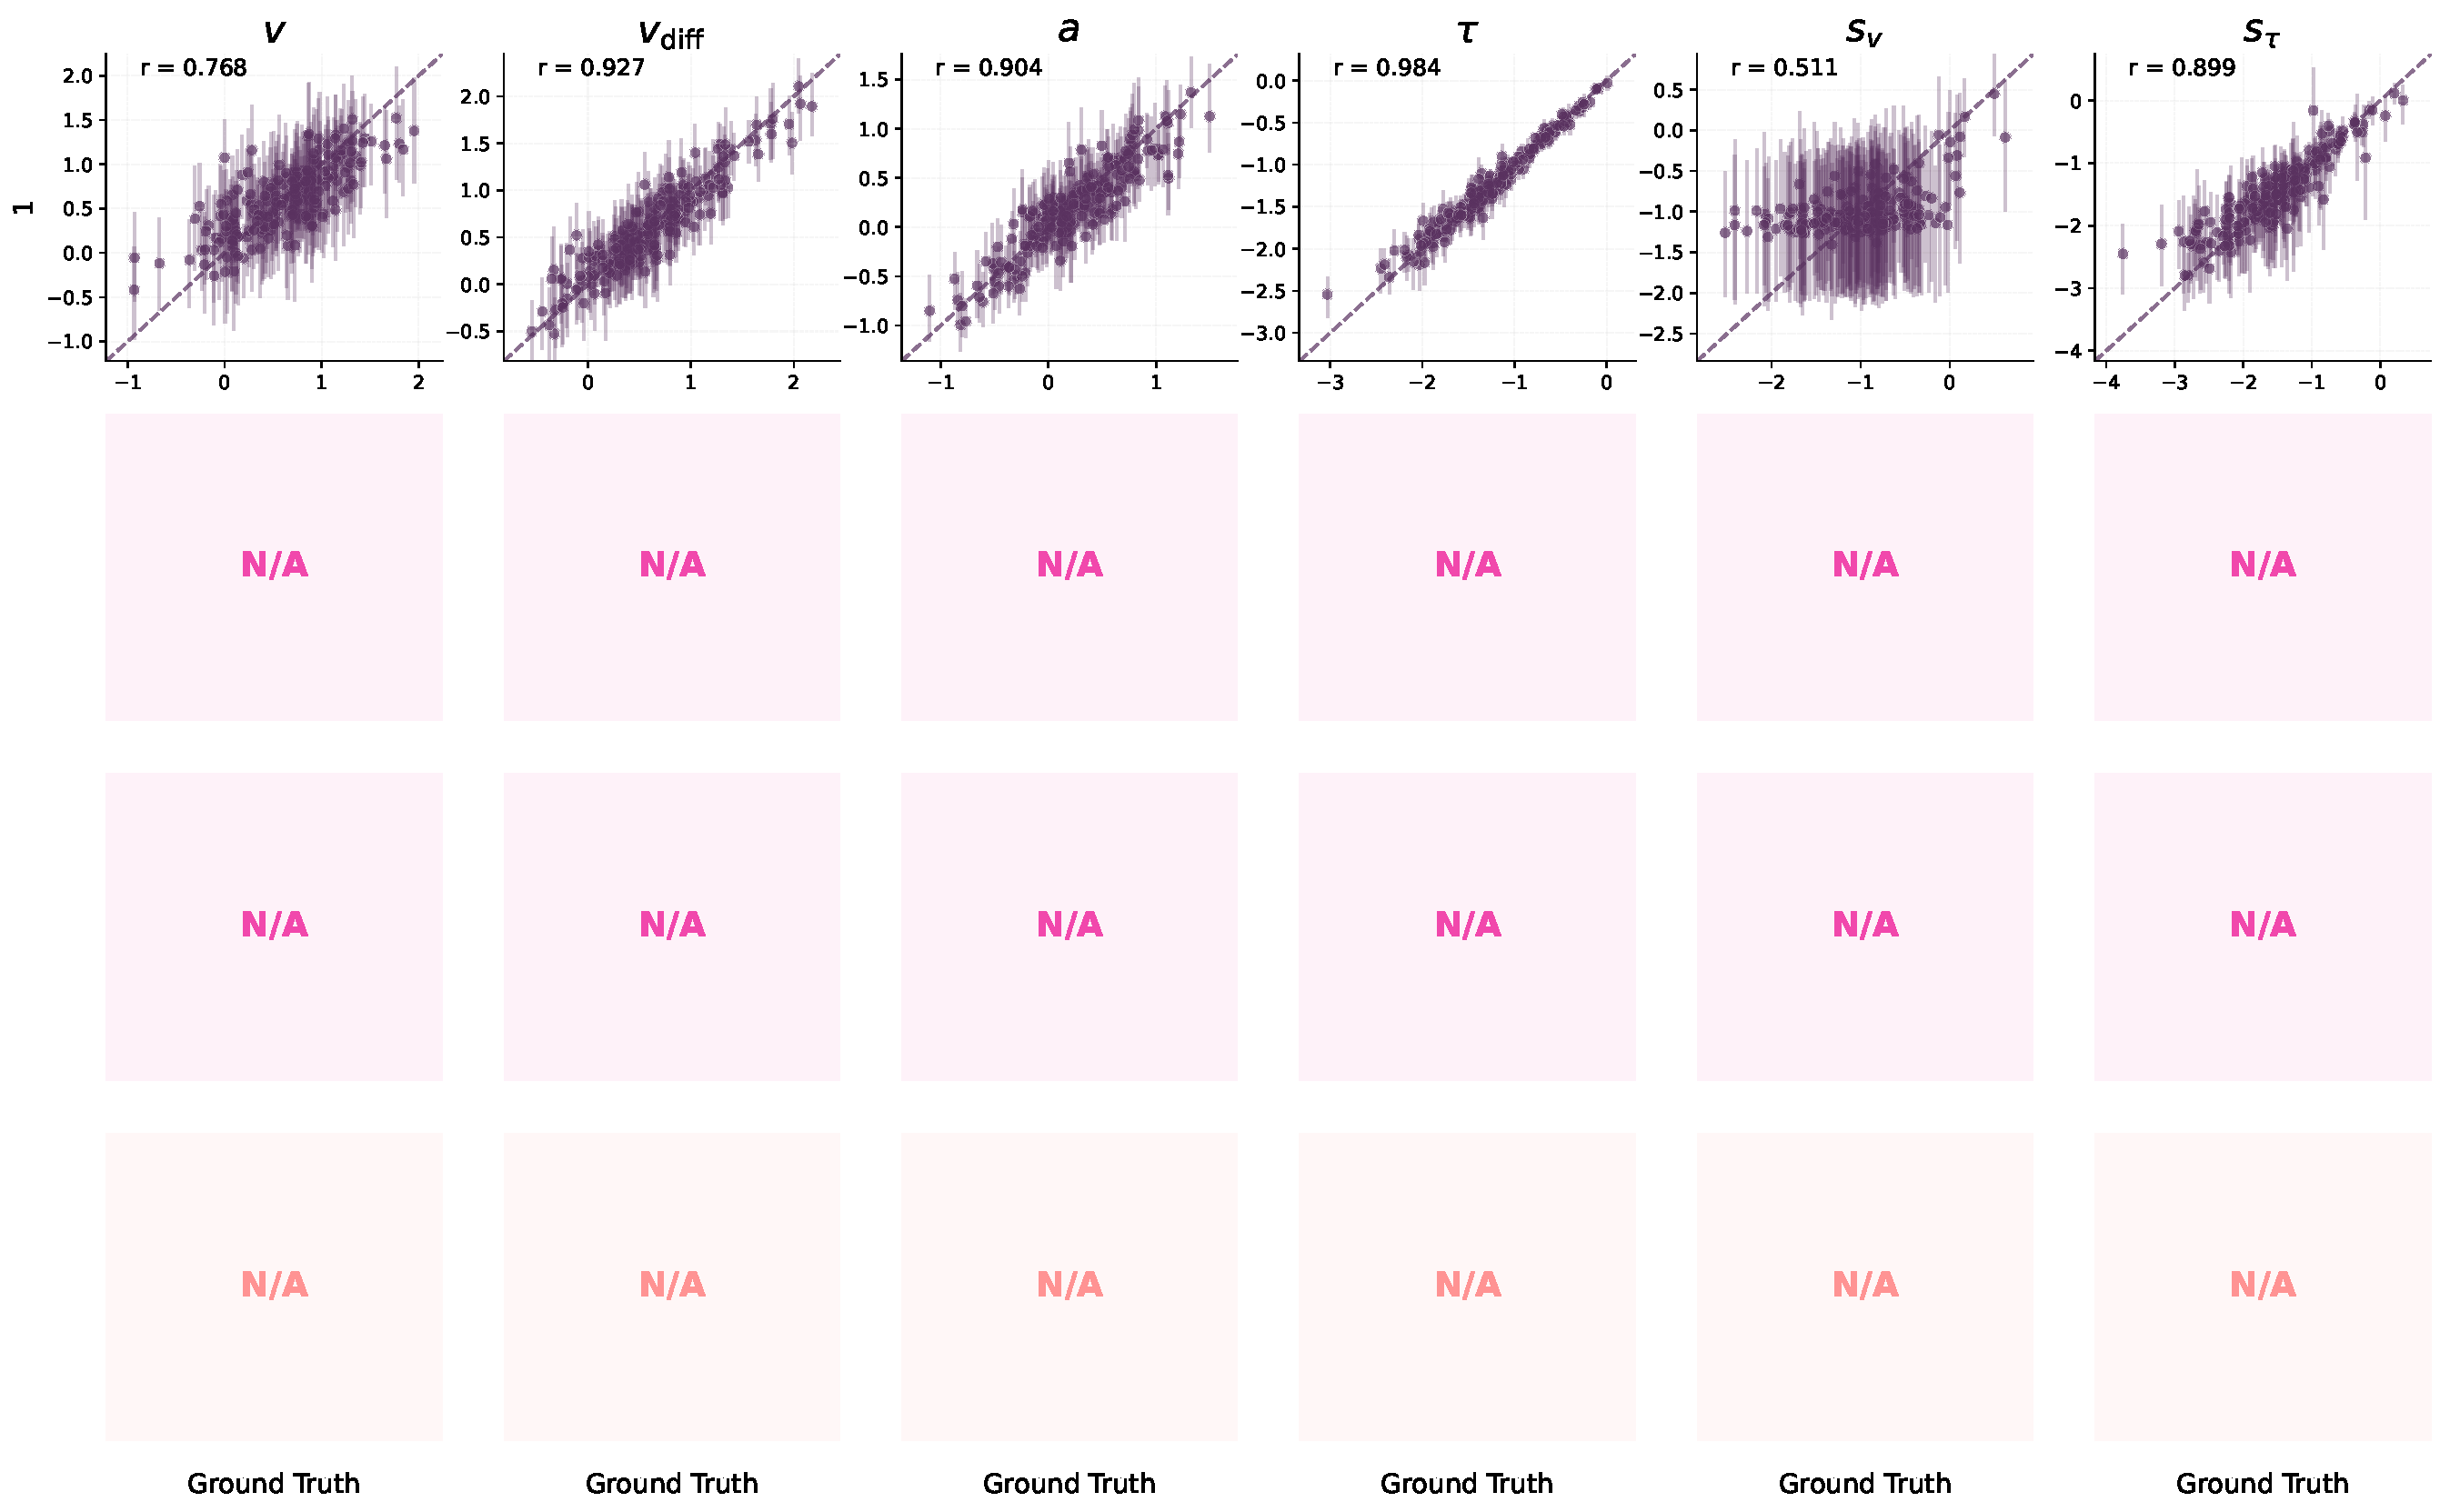
\includegraphics[width=0.99\linewidth]{figures/fm/rdm/intercept_only/rdm_family_intercept_only_fm_mixed_recovery.pdf}
    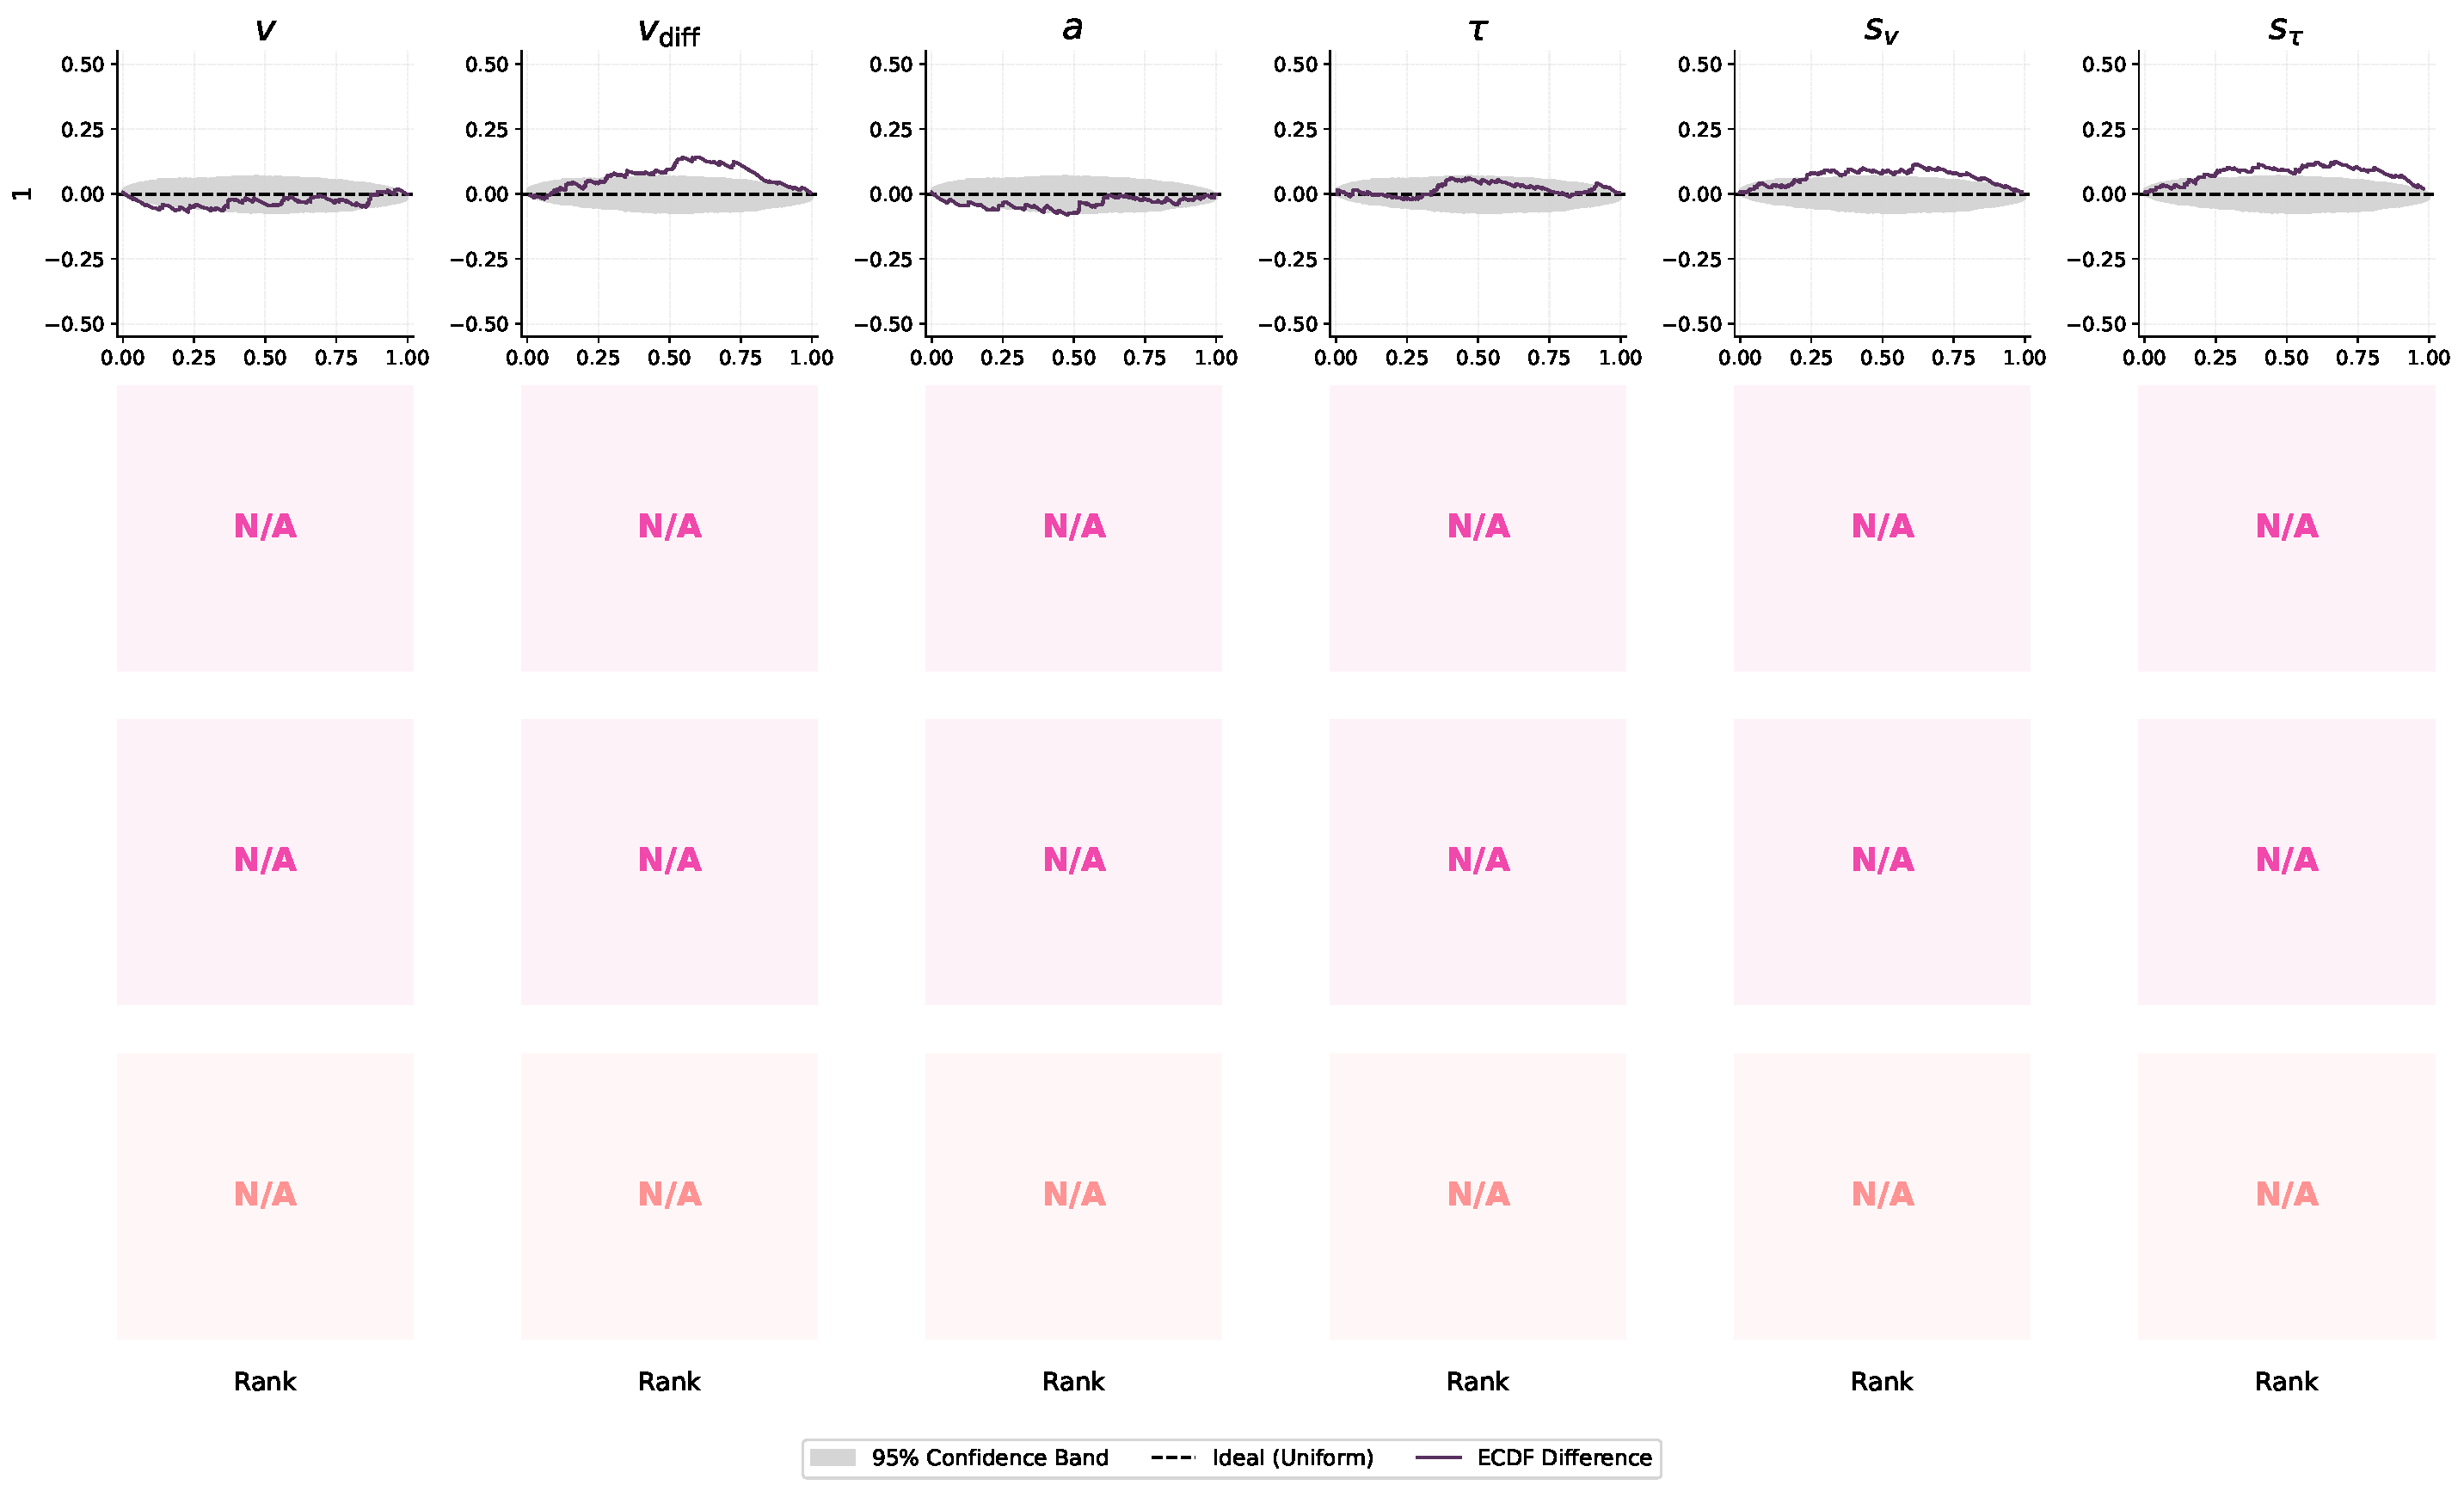
\includegraphics[width=0.99\linewidth]{figures/fm/rdm/intercept_only/rdm_family_intercept_only_fm_mixed_ecdf.pdf}
    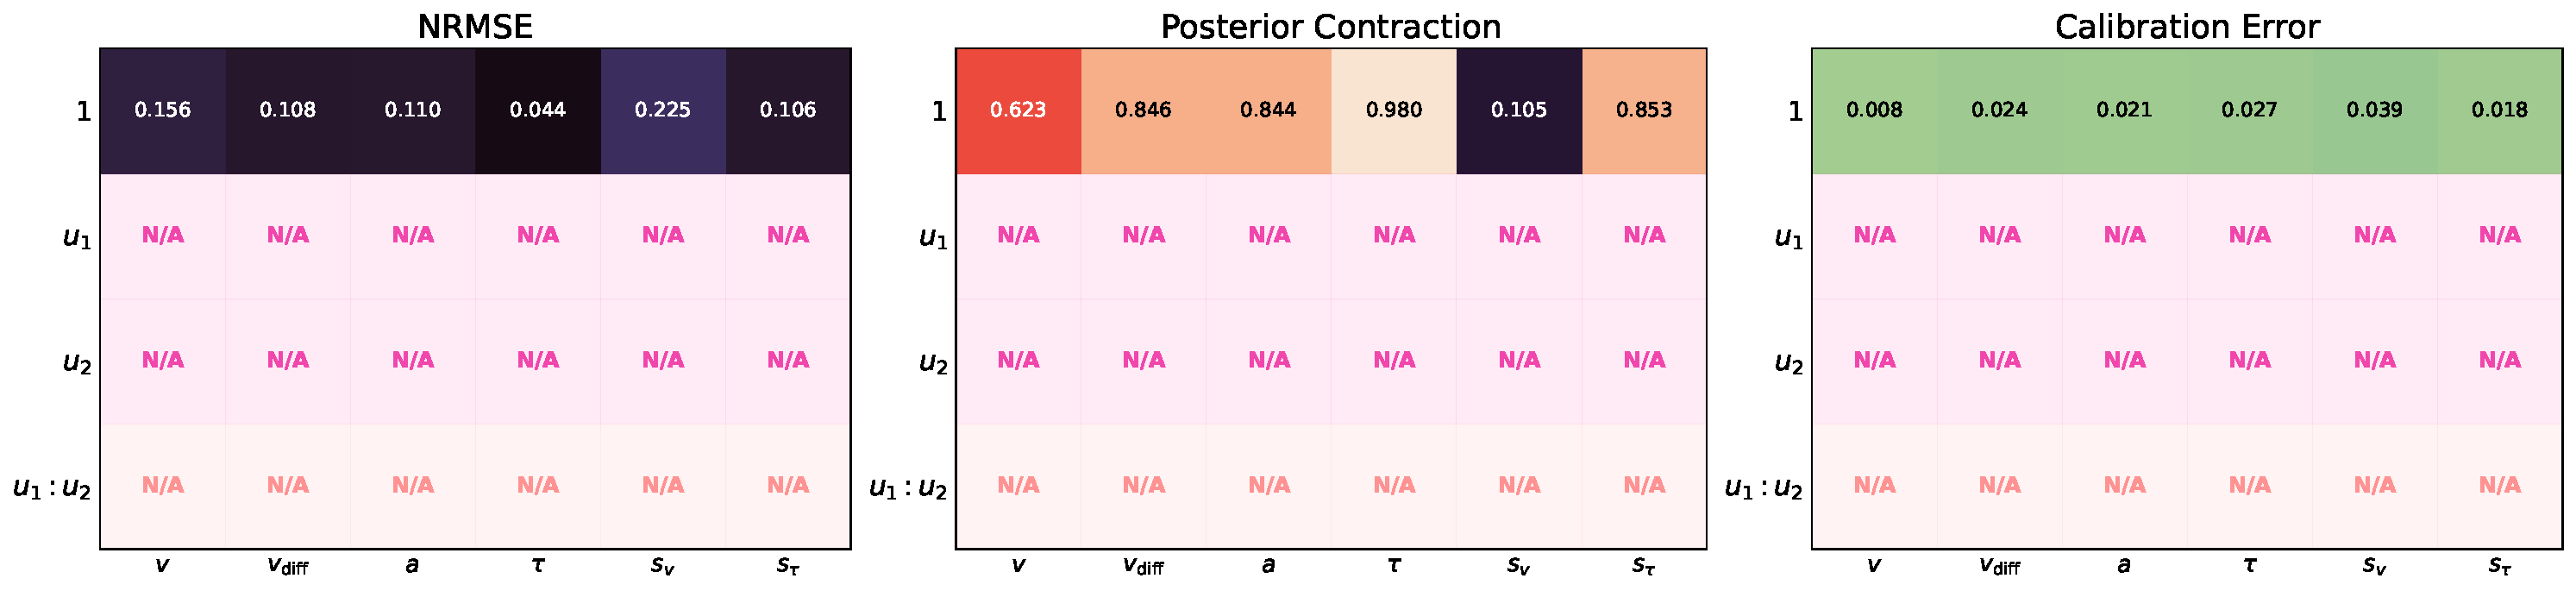
\includegraphics[width=0.99\linewidth]{figures/fm/rdm/intercept_only/rdm_family_intercept_only_fm_mixed_metrics.pdf}
    \caption{Parameter recovery (\emph{top}), calibration ECDF (\emph{middle}), and parameter-wise metrics (NRMSE, calibration error, and posterior contraction) for RDM model family (Case \textbf{intercept\_only}).}
    \label{fig:rdm-fm-intercept-only}
\end{figure}

\begin{figure}
    \centering
    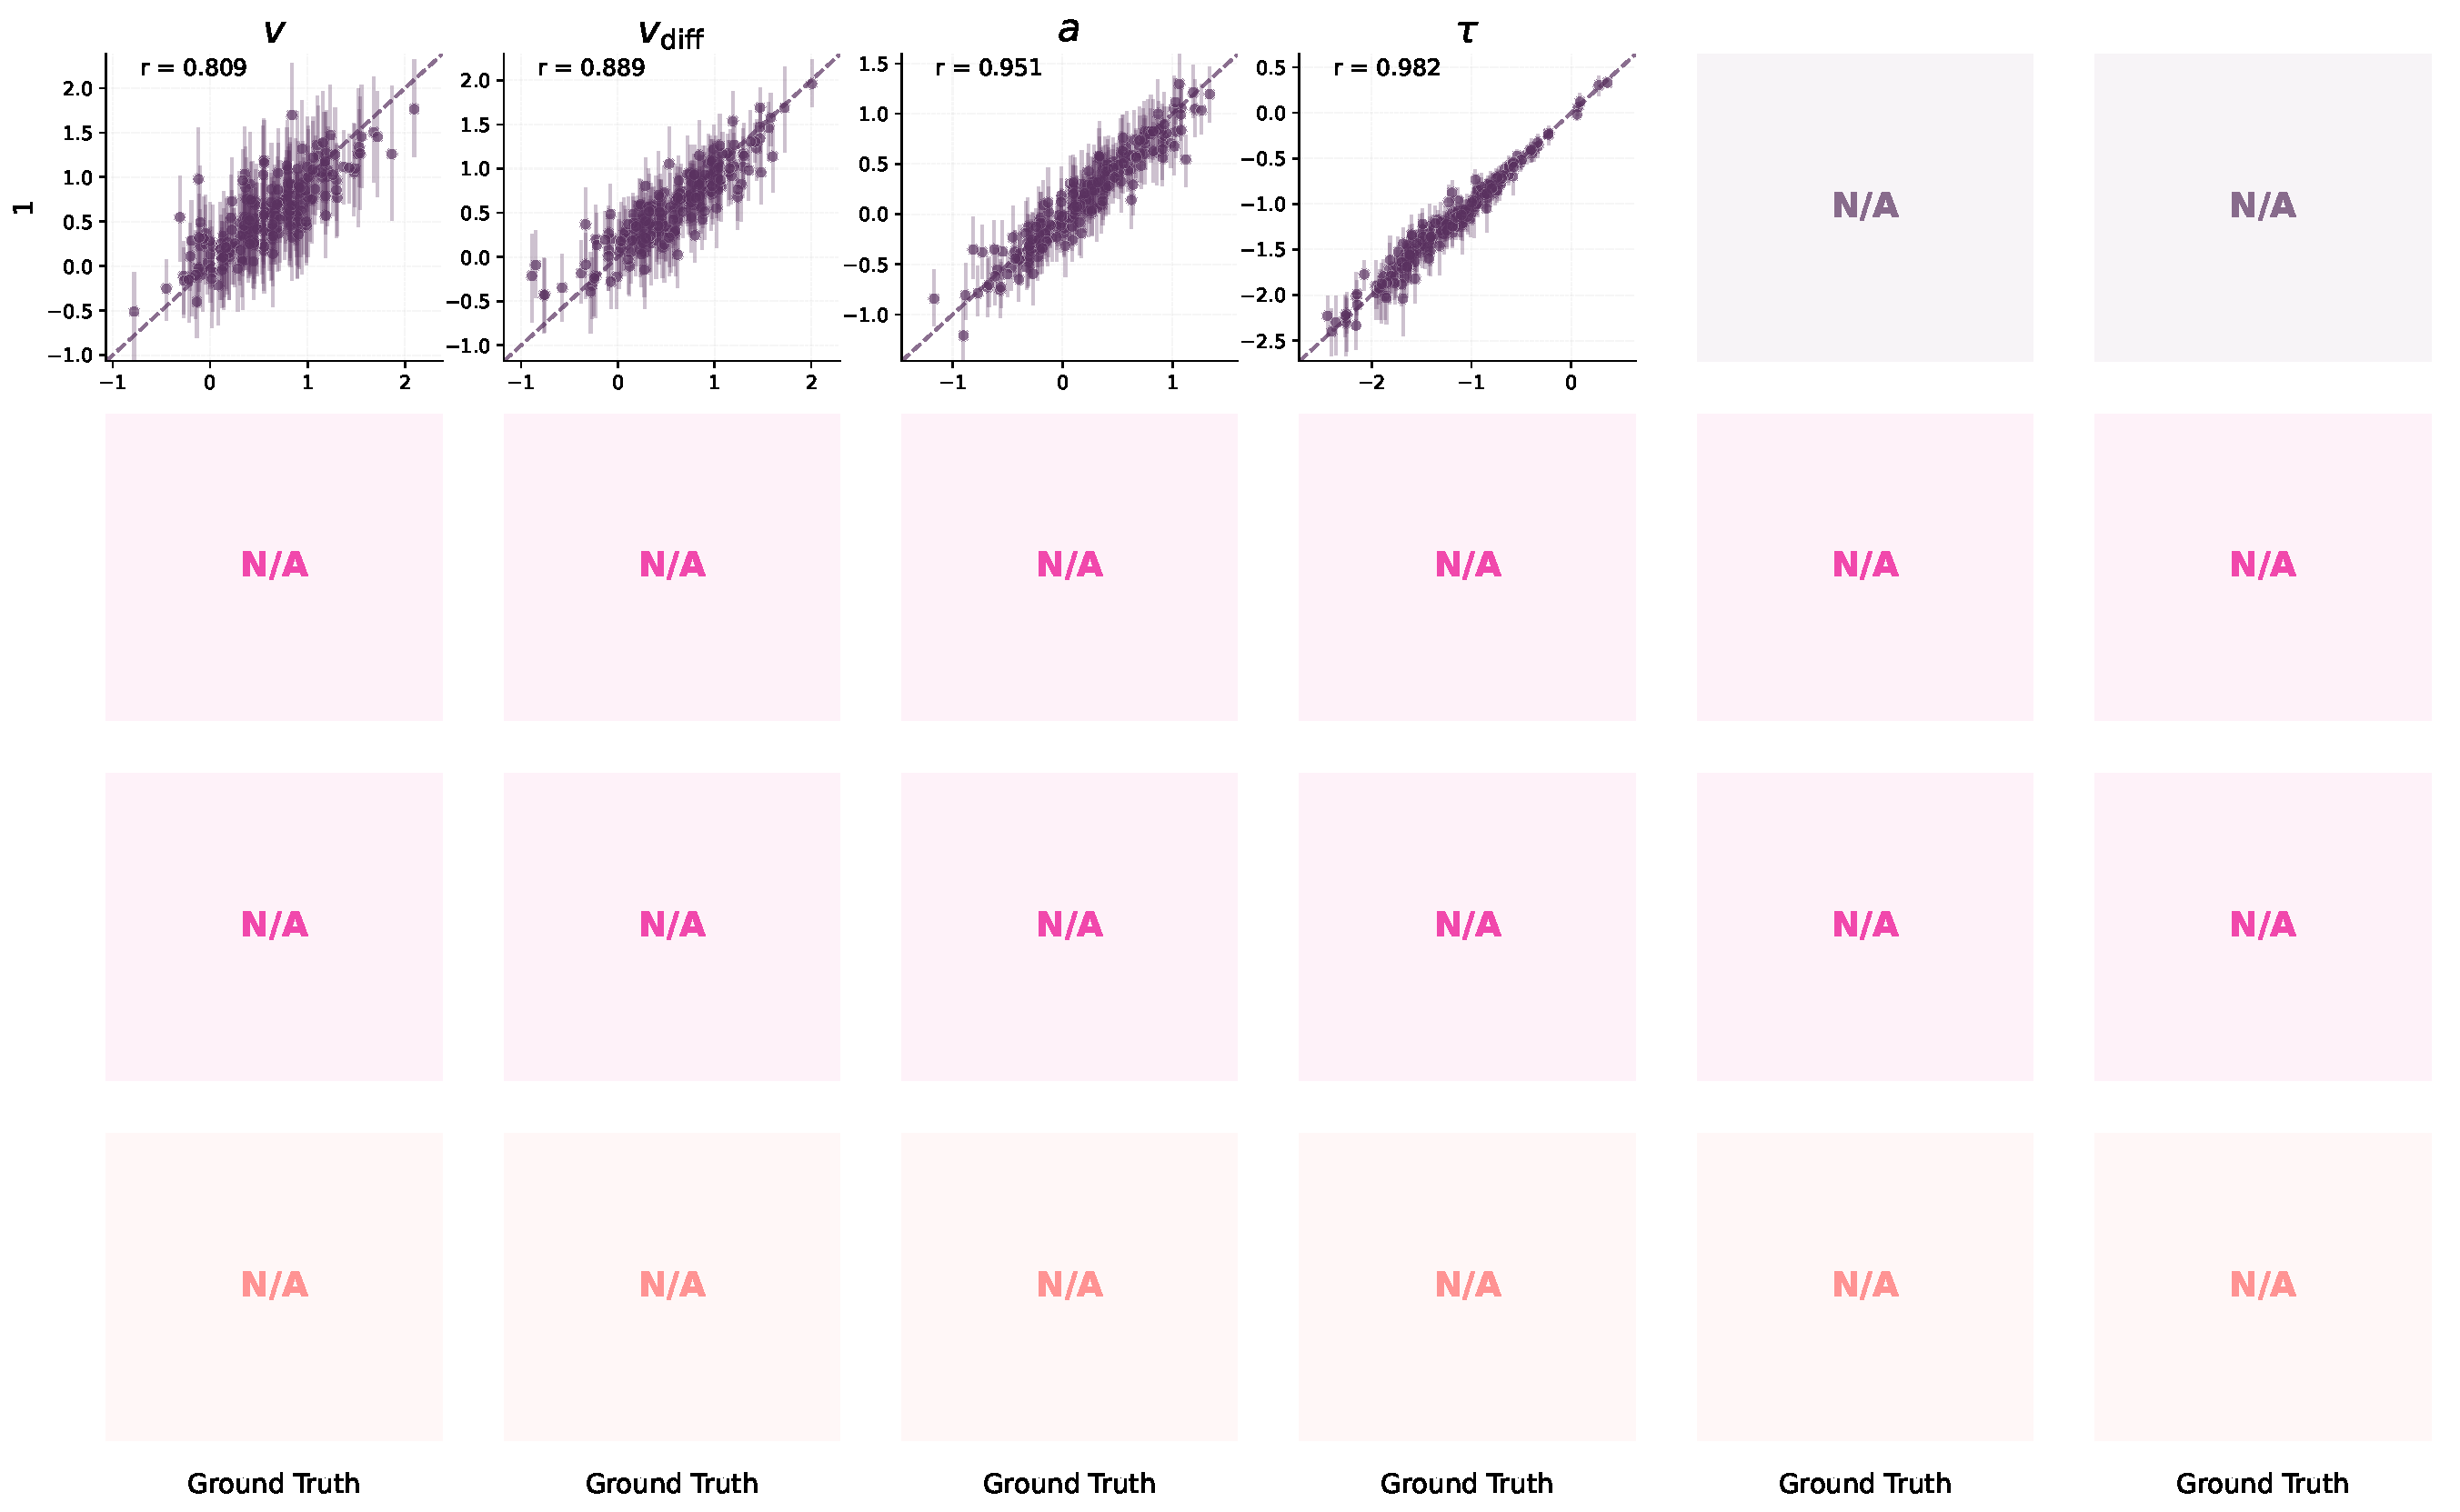
\includegraphics[width=0.99\linewidth]{figures/fm/rdm/fixed/rdm_family_fixed_fm_mixed_recovery.pdf}
    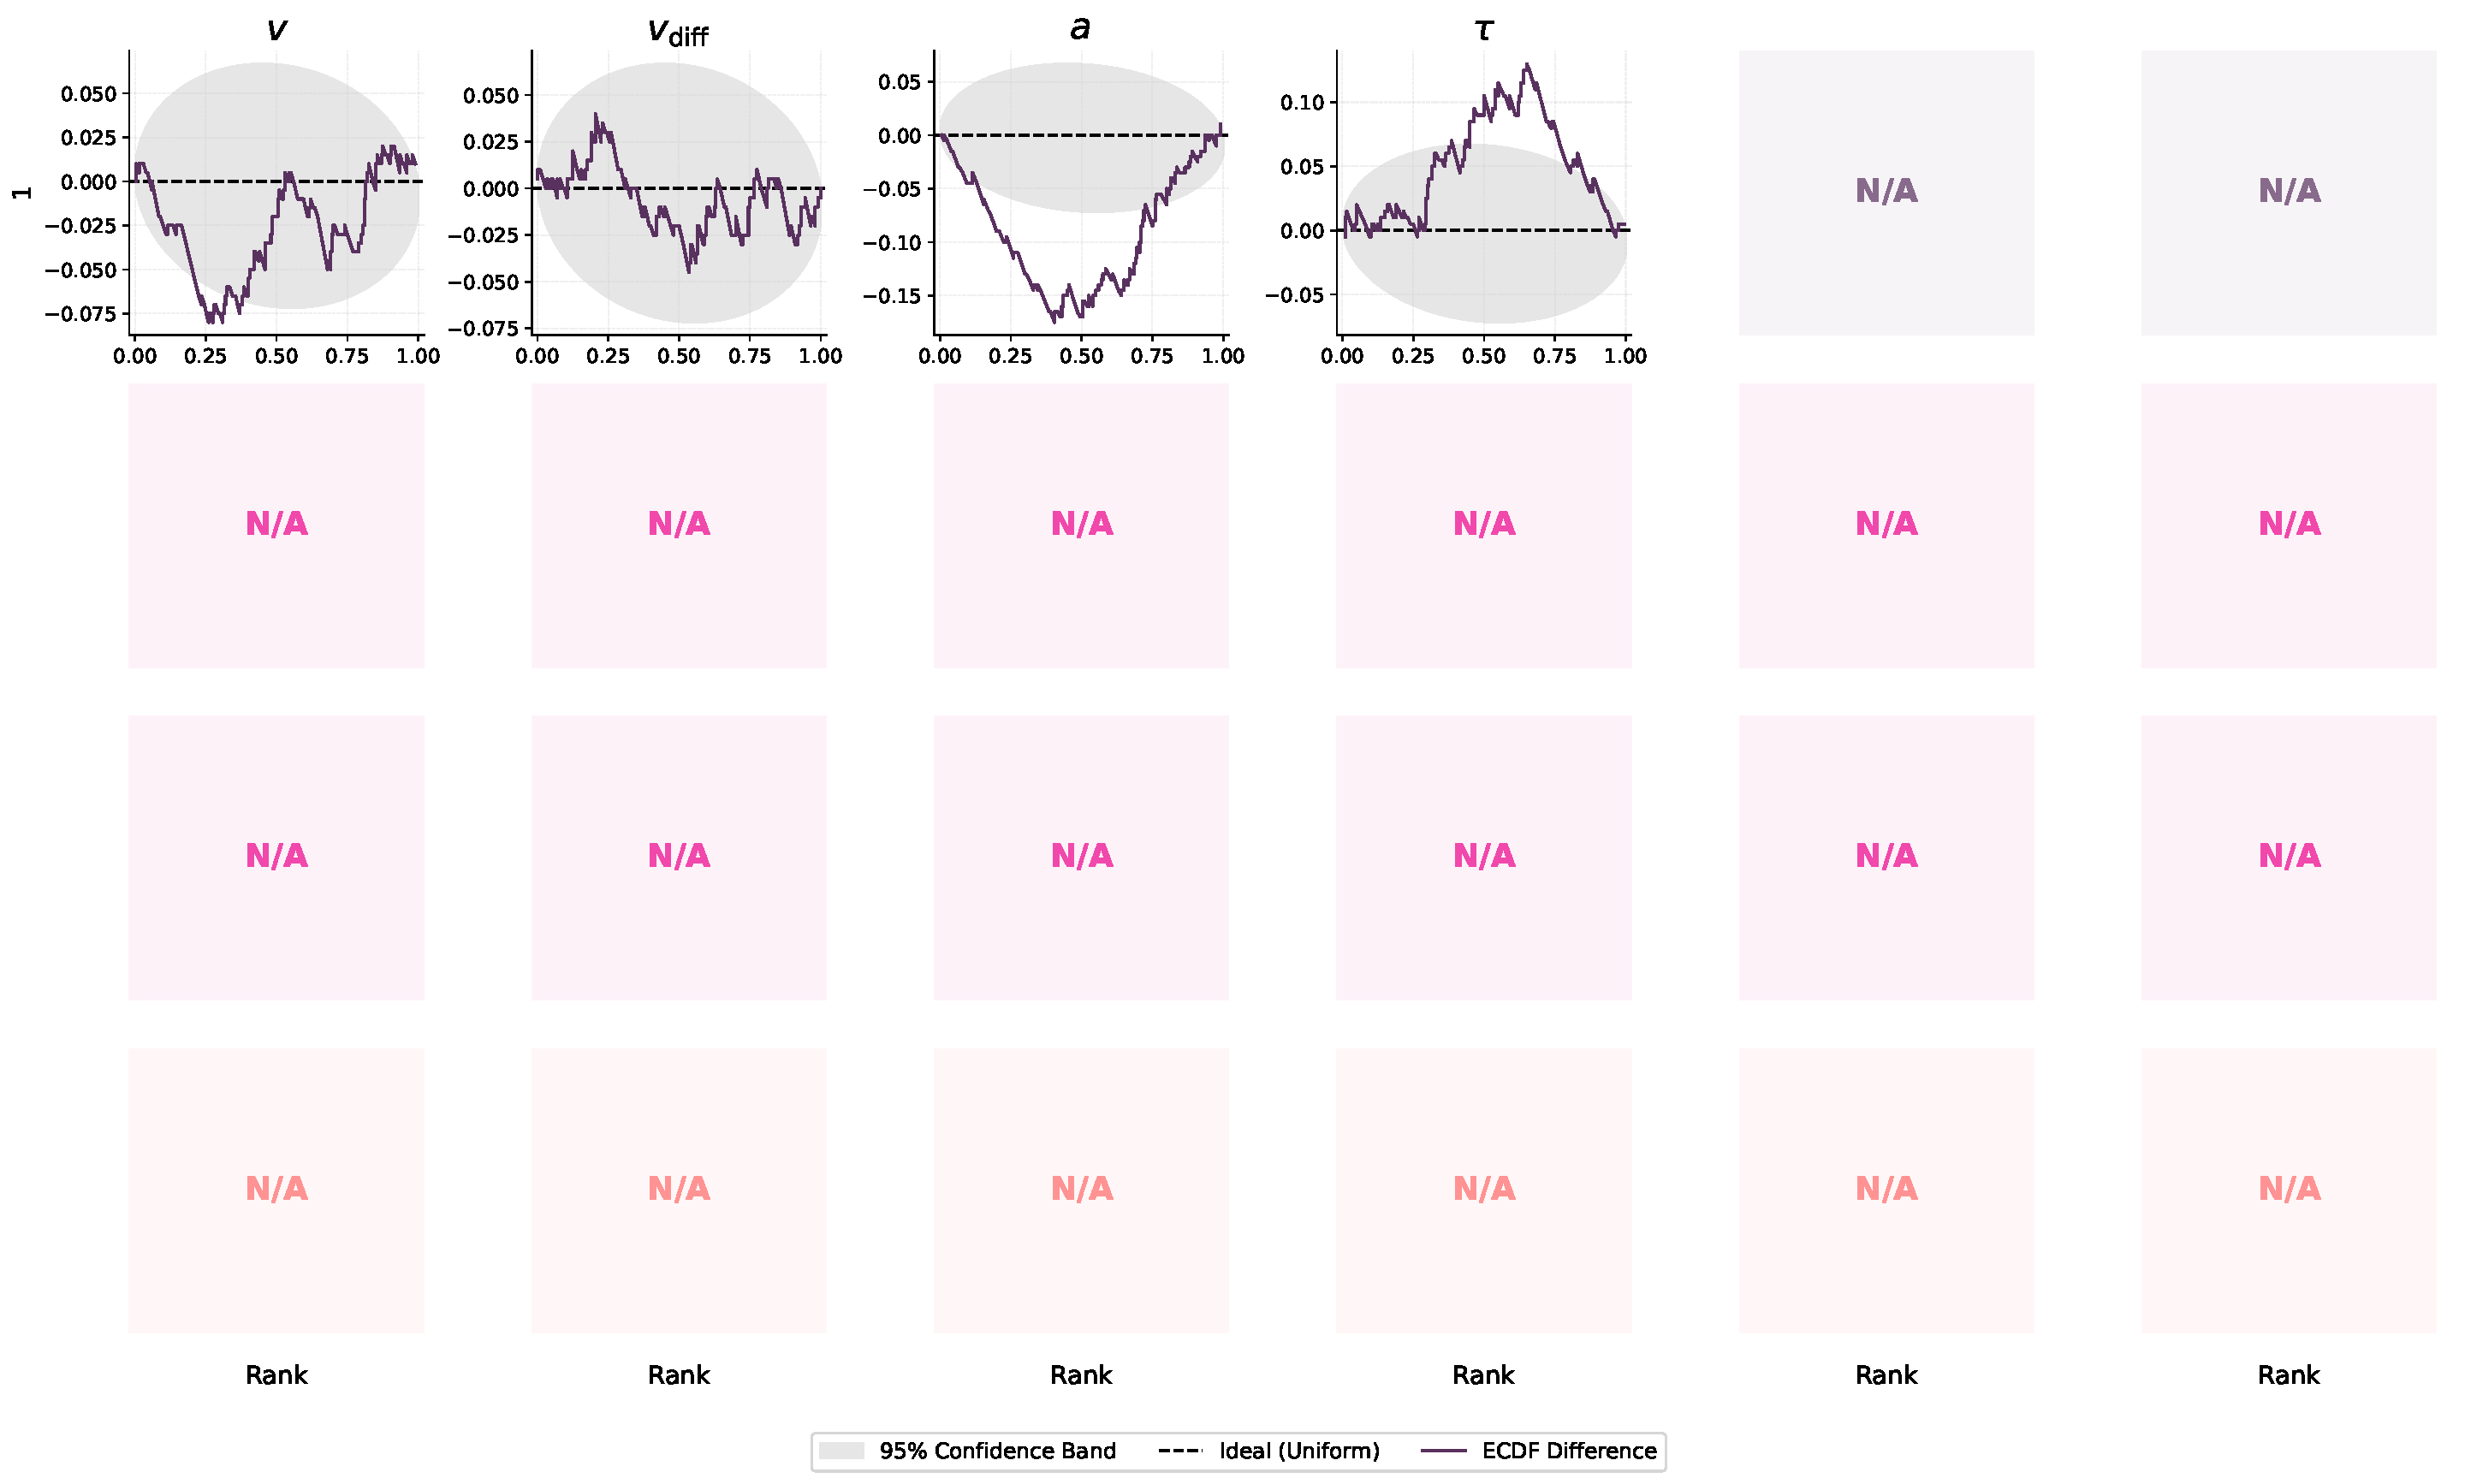
\includegraphics[width=0.99\linewidth]{figures/fm/rdm/fixed/rdm_family_fixed_fm_mixed_ecdf.pdf}
    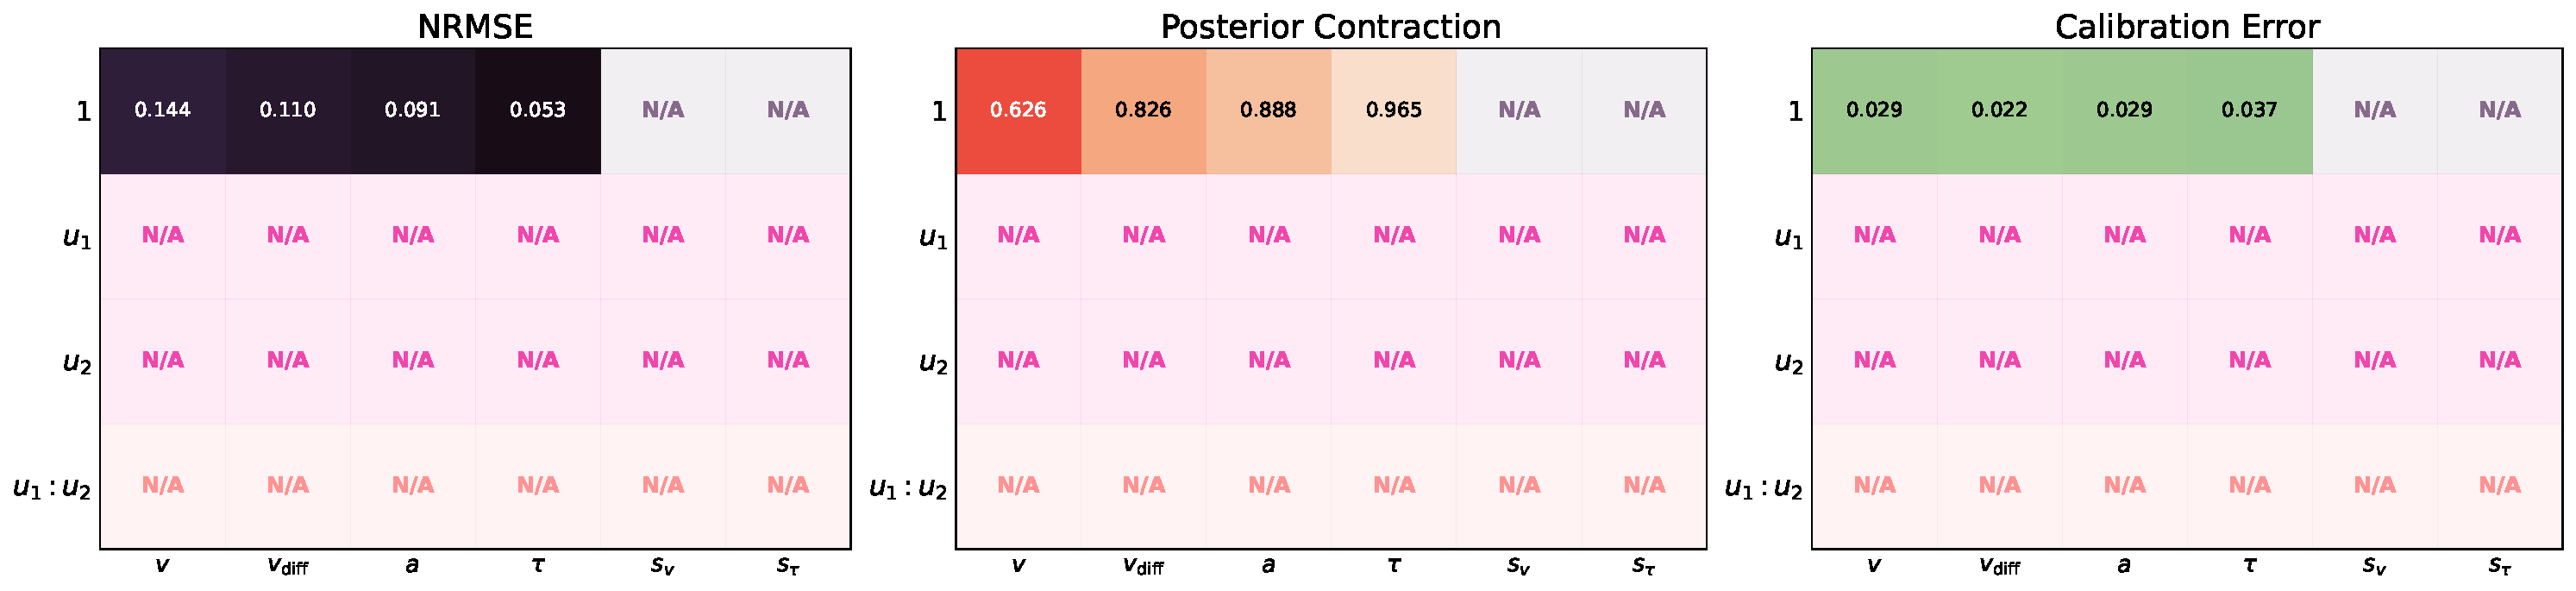
\includegraphics[width=0.99\linewidth]{figures/fm/rdm/fixed/rdm_family_fixed_fm_mixed_metrics.pdf}
    \caption{Parameter recovery (\emph{top}), calibration ECDF (\emph{middle}), and parameter-wise metrics (NRMSE, calibration error, and posterior contraction) for RDM model family (Case \textbf{fixed}).}
    \label{fig:rdm-fm-fixed}
\end{figure}

\begin{figure}
    \centering
    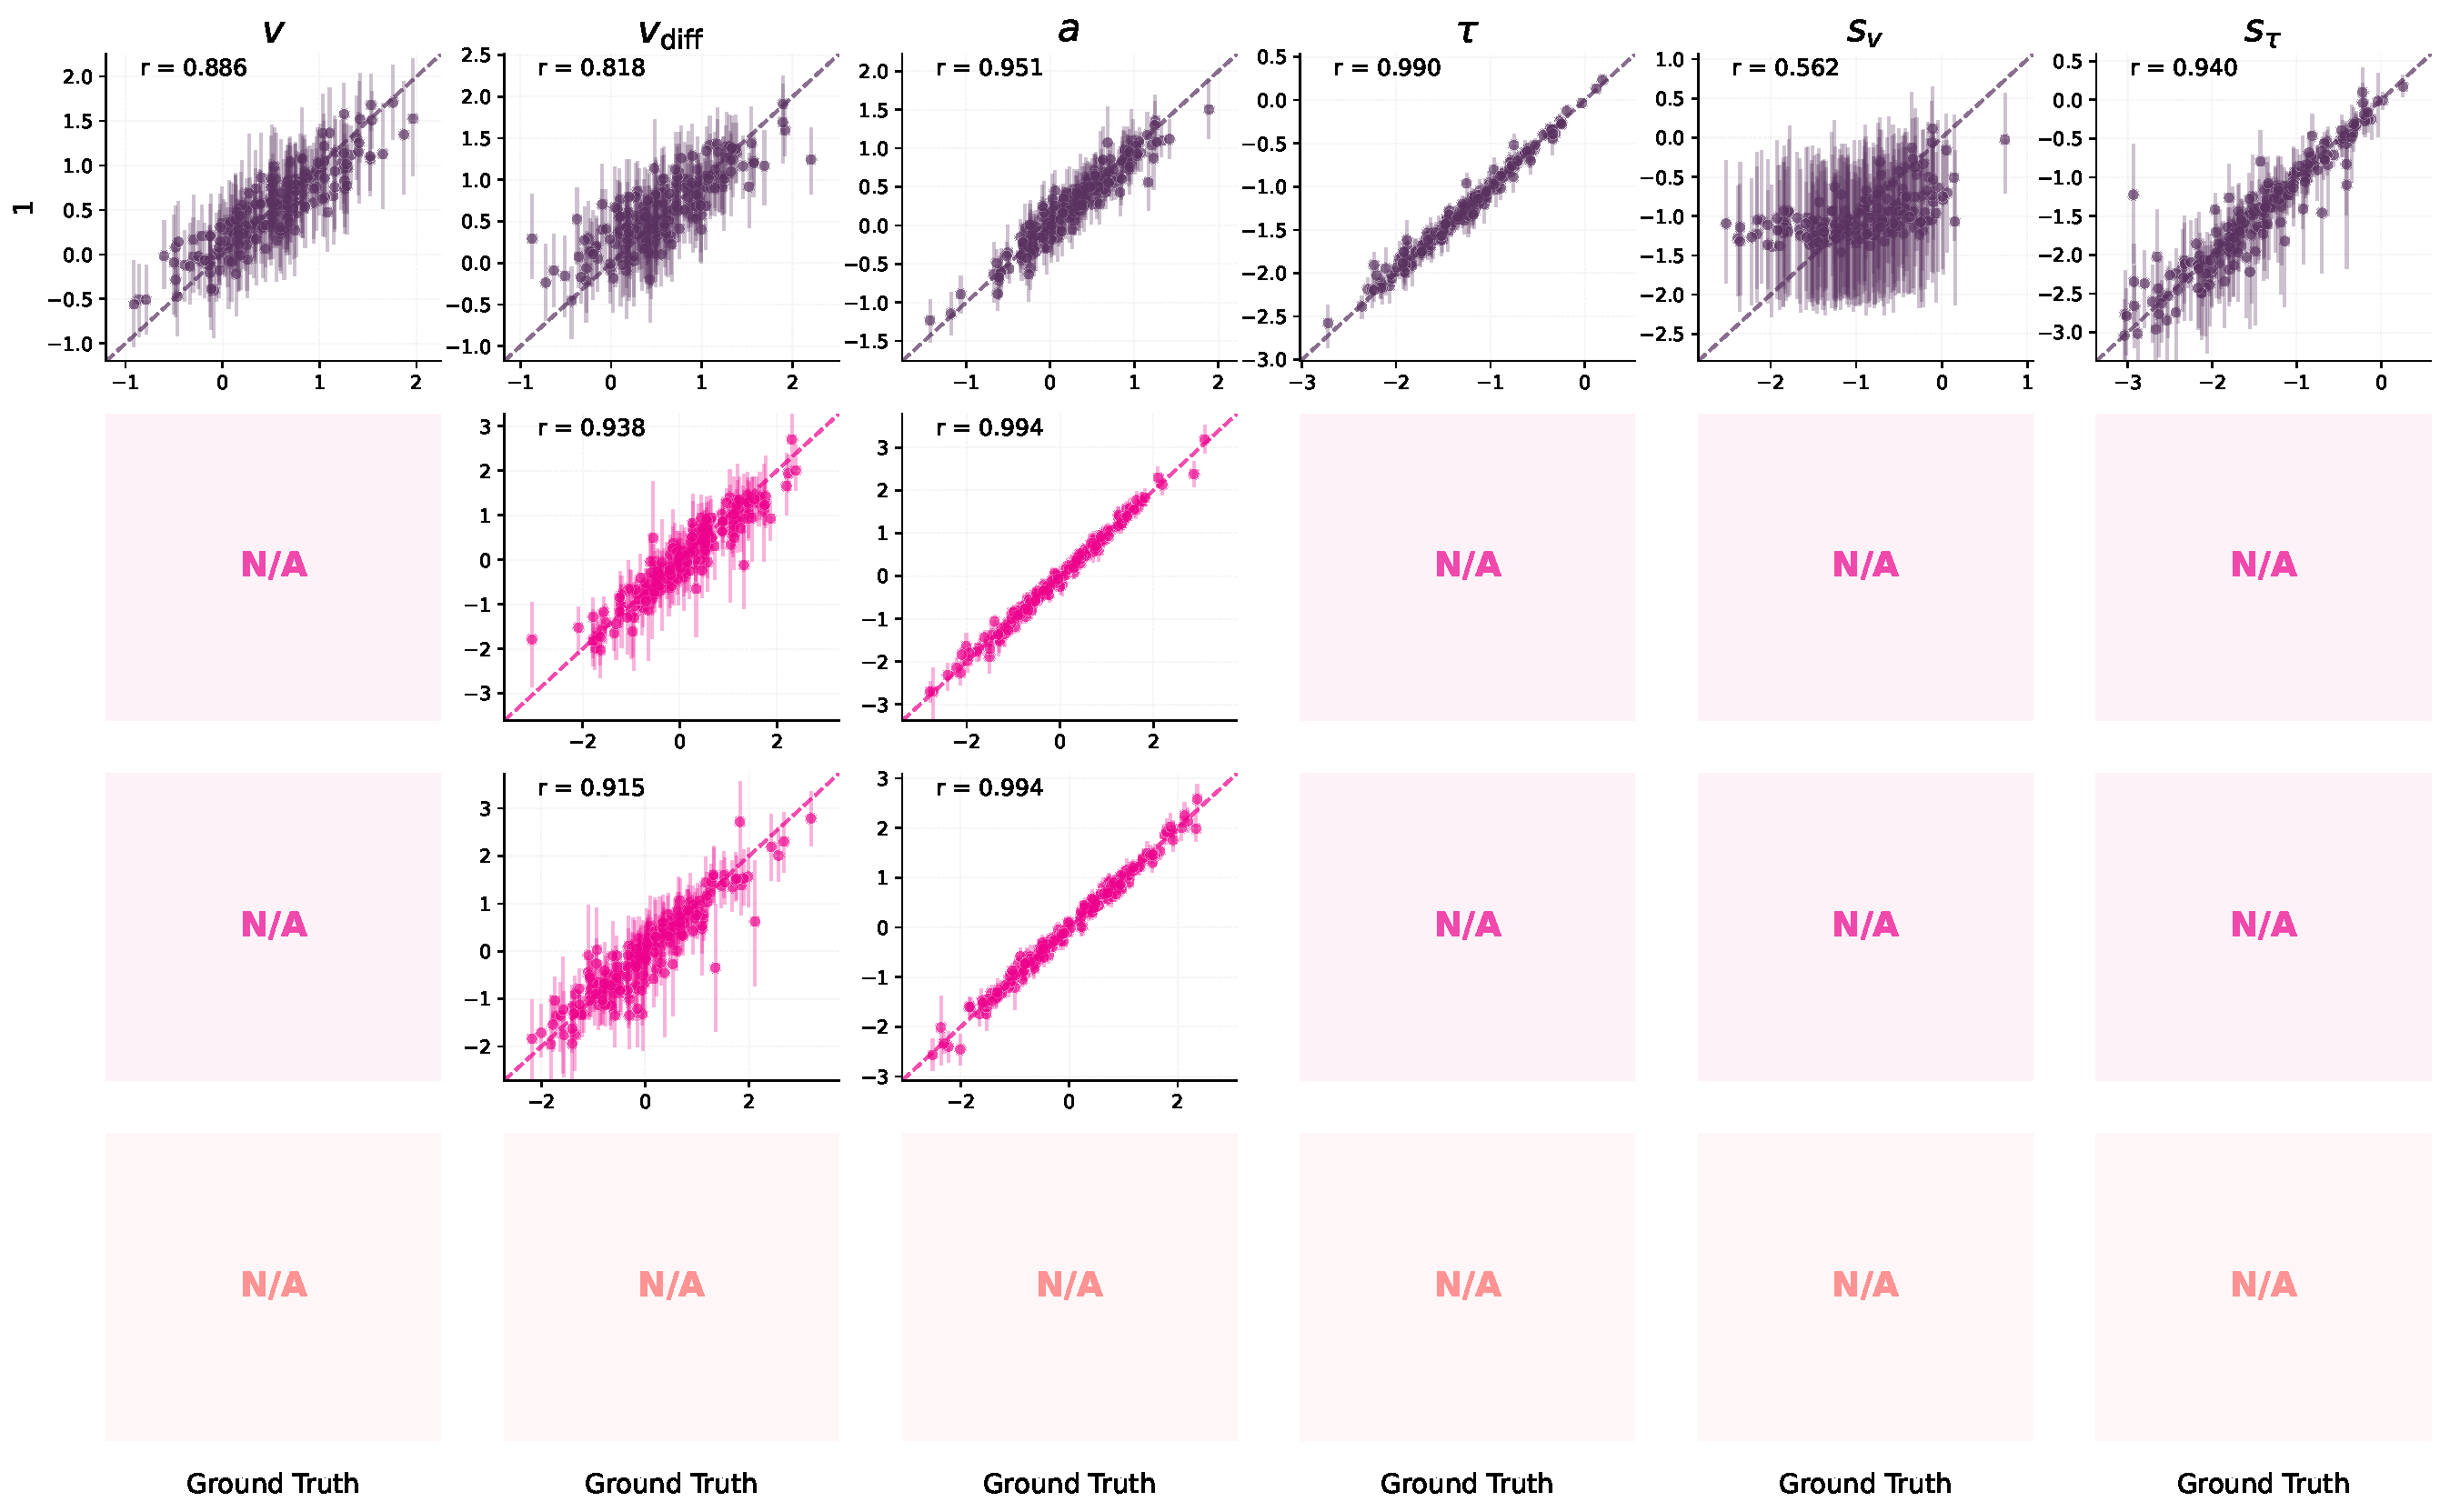
\includegraphics[width=0.99\linewidth]{figures/fm/rdm/regressed/rdm_family_regressed_fm_mixed_recovery.pdf}
    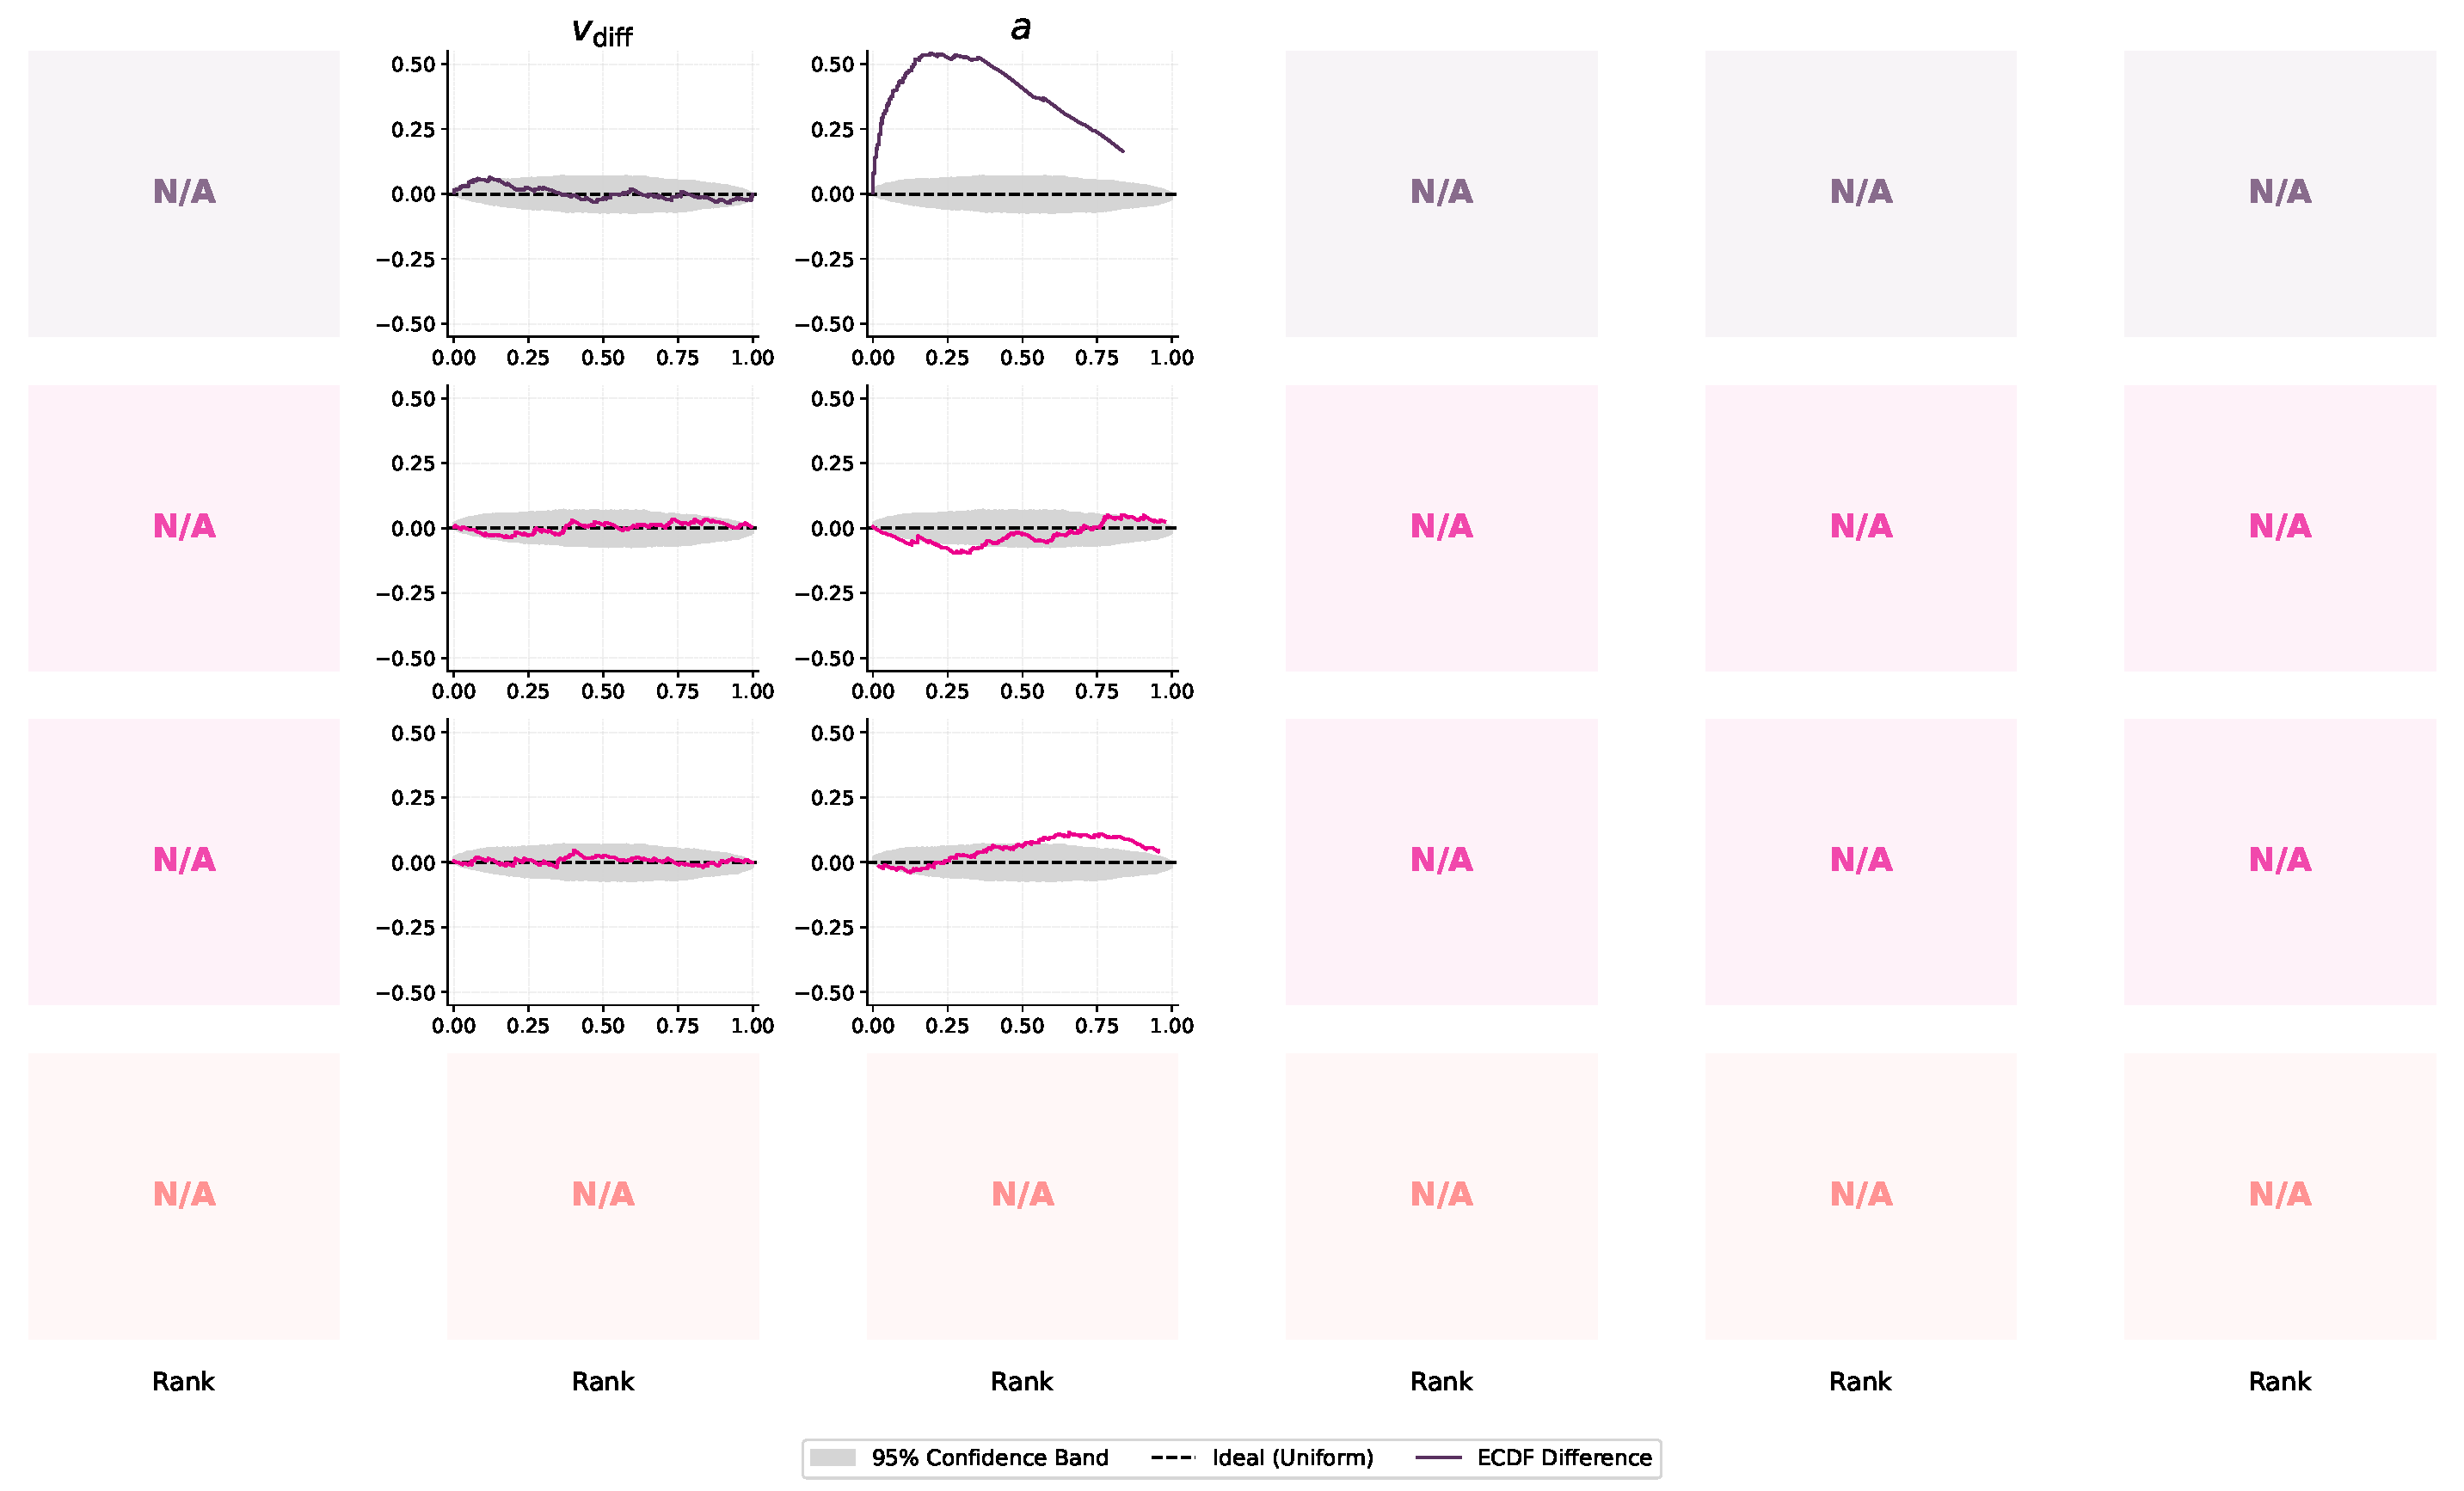
\includegraphics[width=0.99\linewidth]{figures/fm/rdm/regressed/rdm_family_regressed_fm_mixed_ecdf.pdf}
    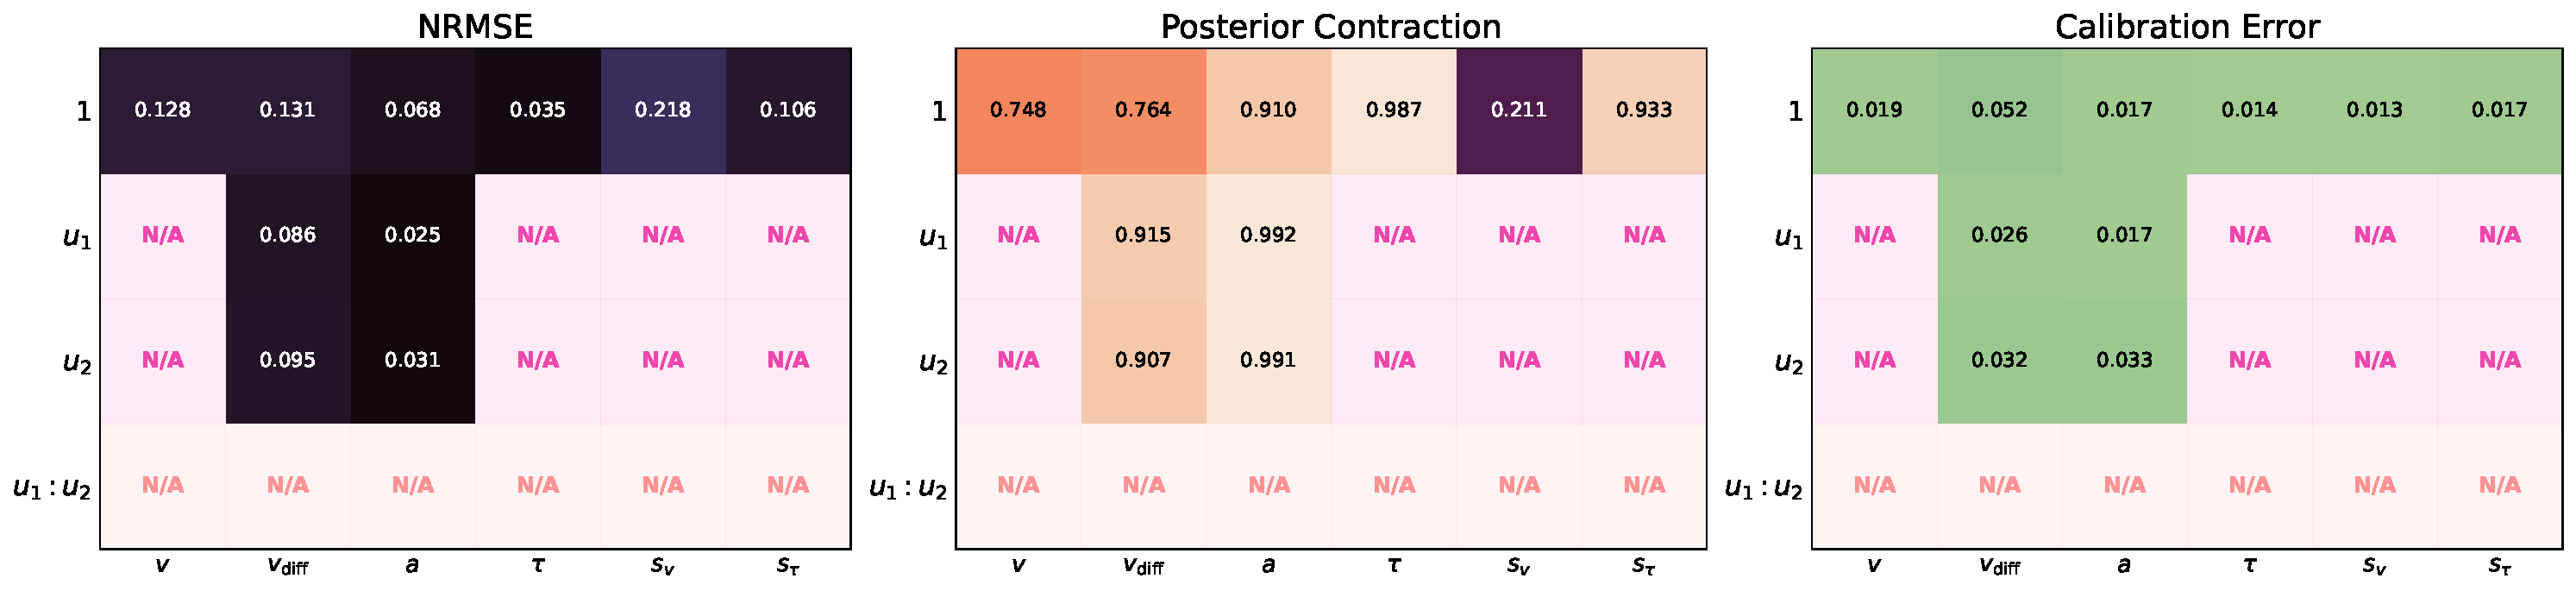
\includegraphics[width=0.99\linewidth]{figures/fm/rdm/regressed/rdm_family_regressed_fm_mixed_metrics.pdf}
    \caption{Parameter recovery (\emph{top}), calibration ECDF (\emph{middle}), and parameter-wise metrics (NRMSE, calibration error, and posterior contraction) for RDM model family (Case \textbf{regressed}).}
    \label{fig:rdm-fm-regressed}
\end{figure}

\begin{figure}
    \centering
    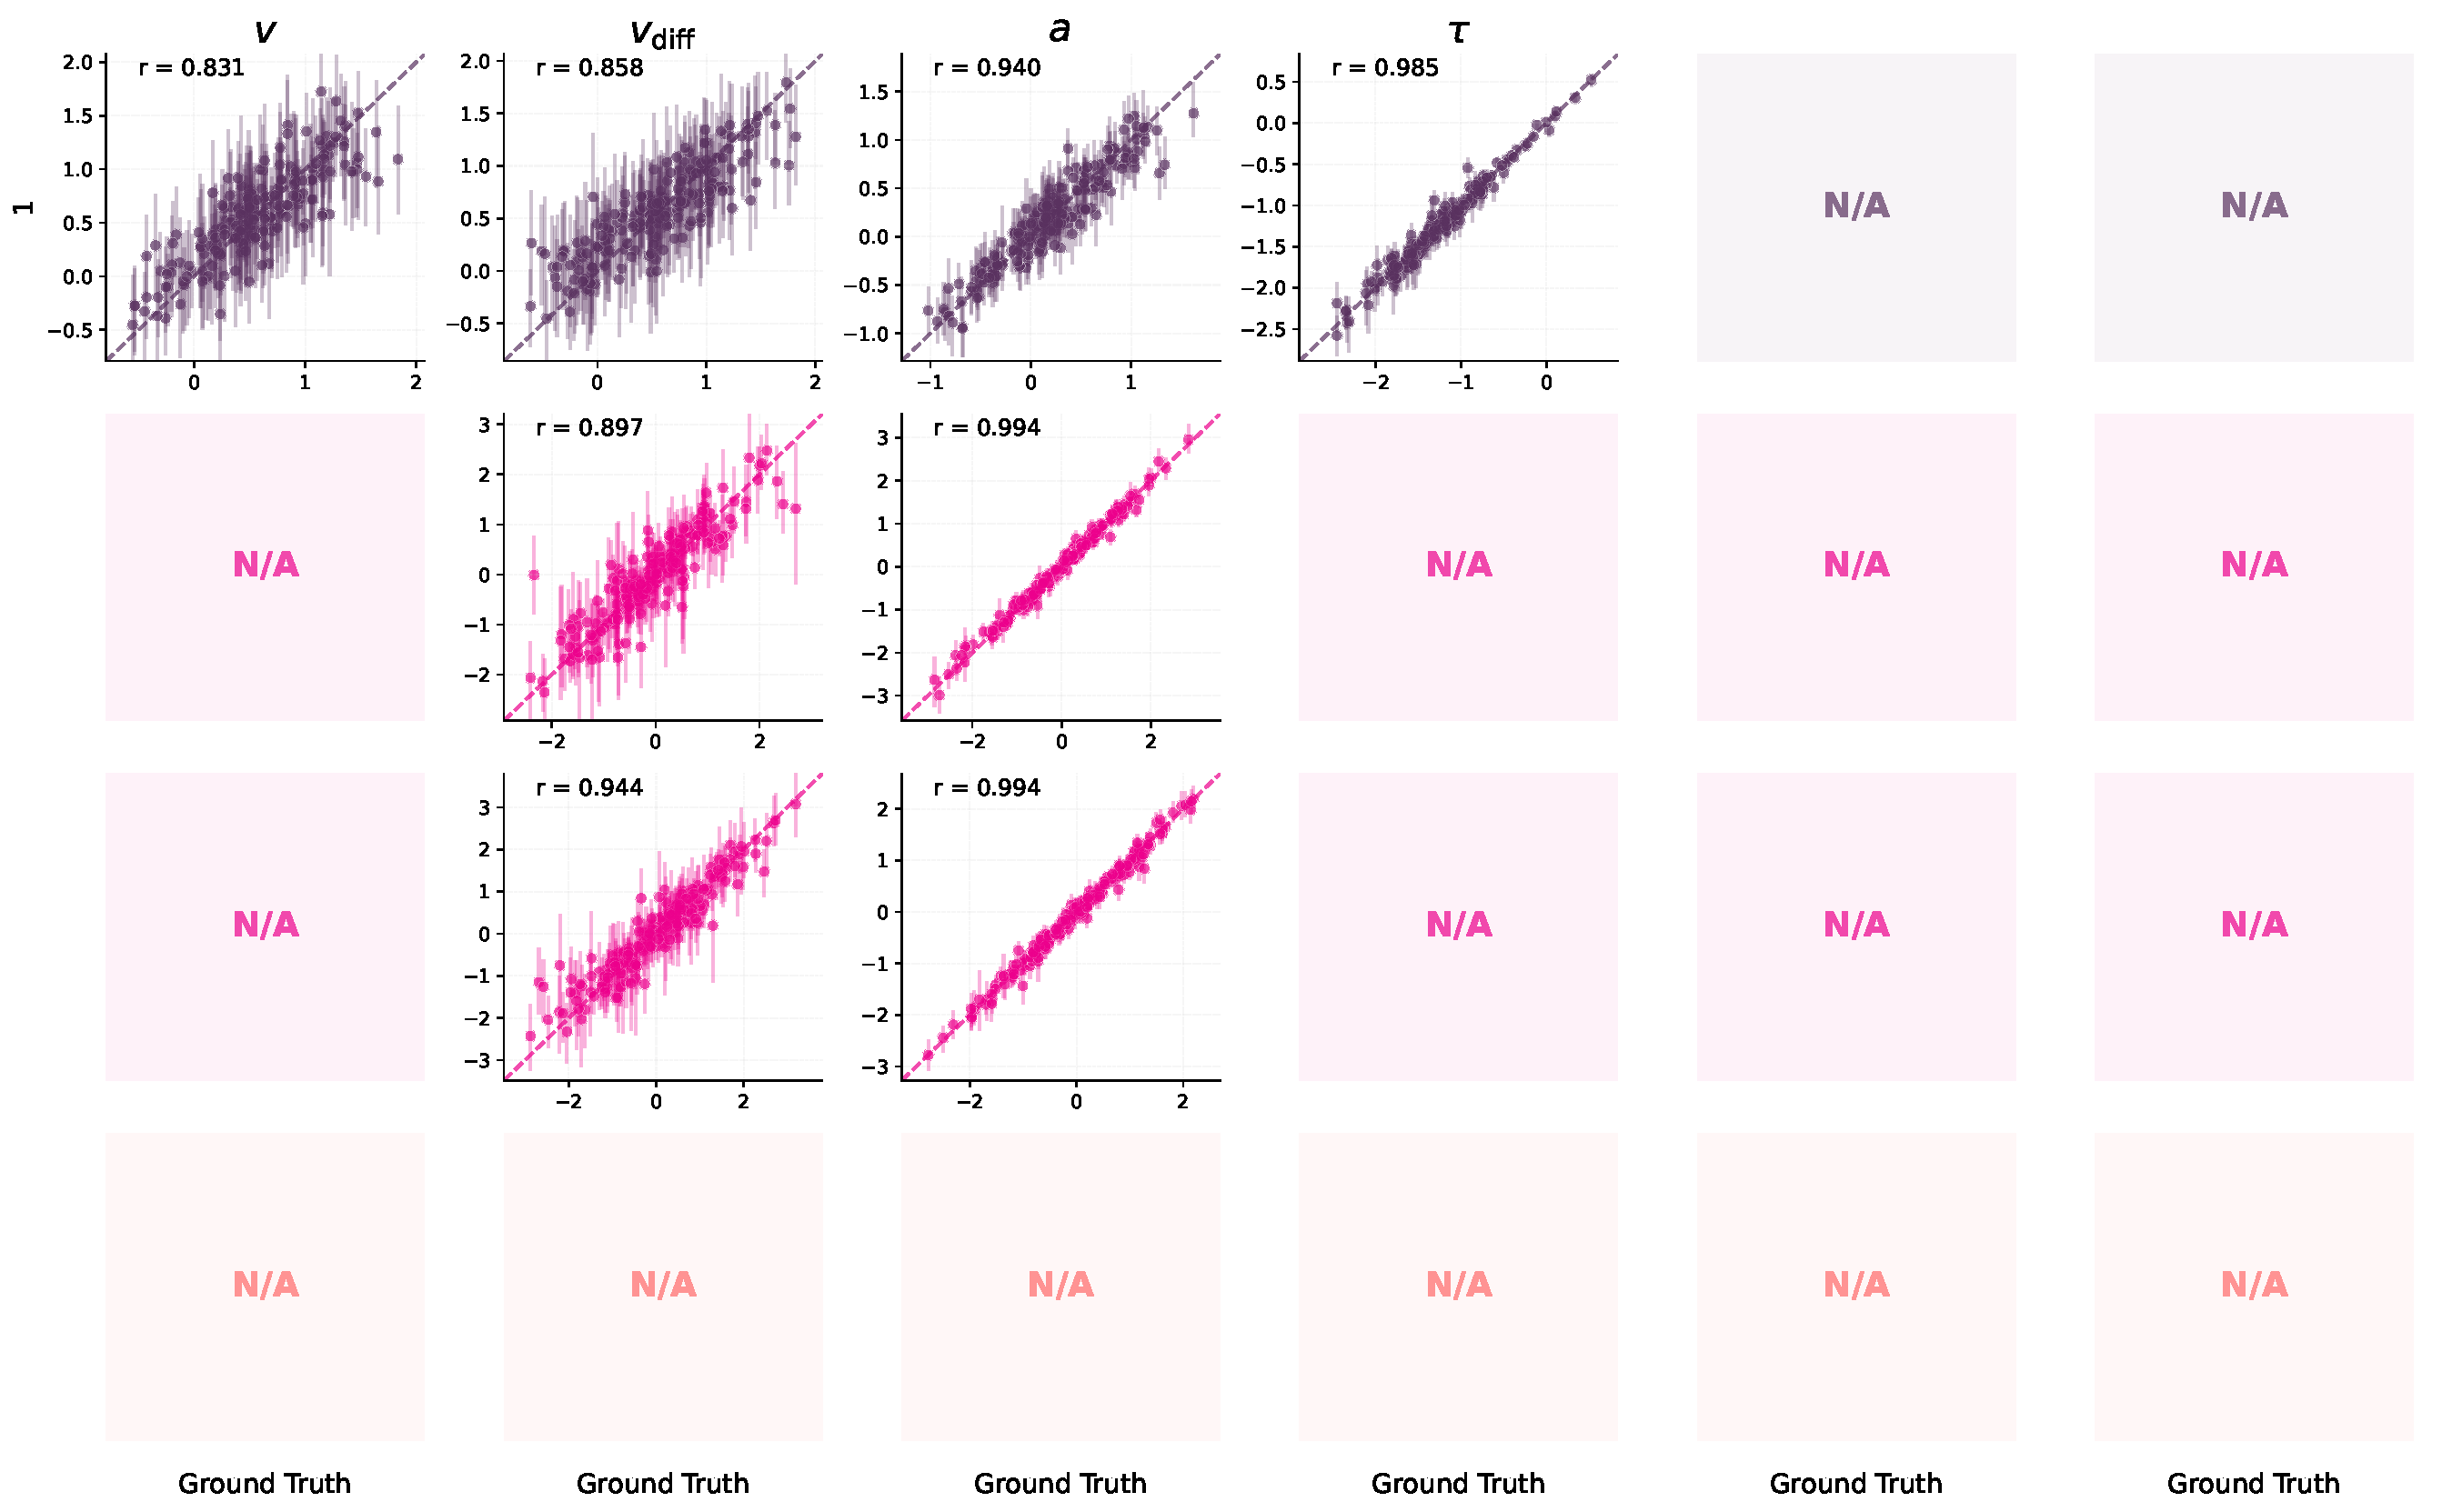
\includegraphics[width=0.99\linewidth]{figures/fm/rdm/fixed_regressed/rdm_family_fixed_regressed_fm_mixed_recovery.pdf}
    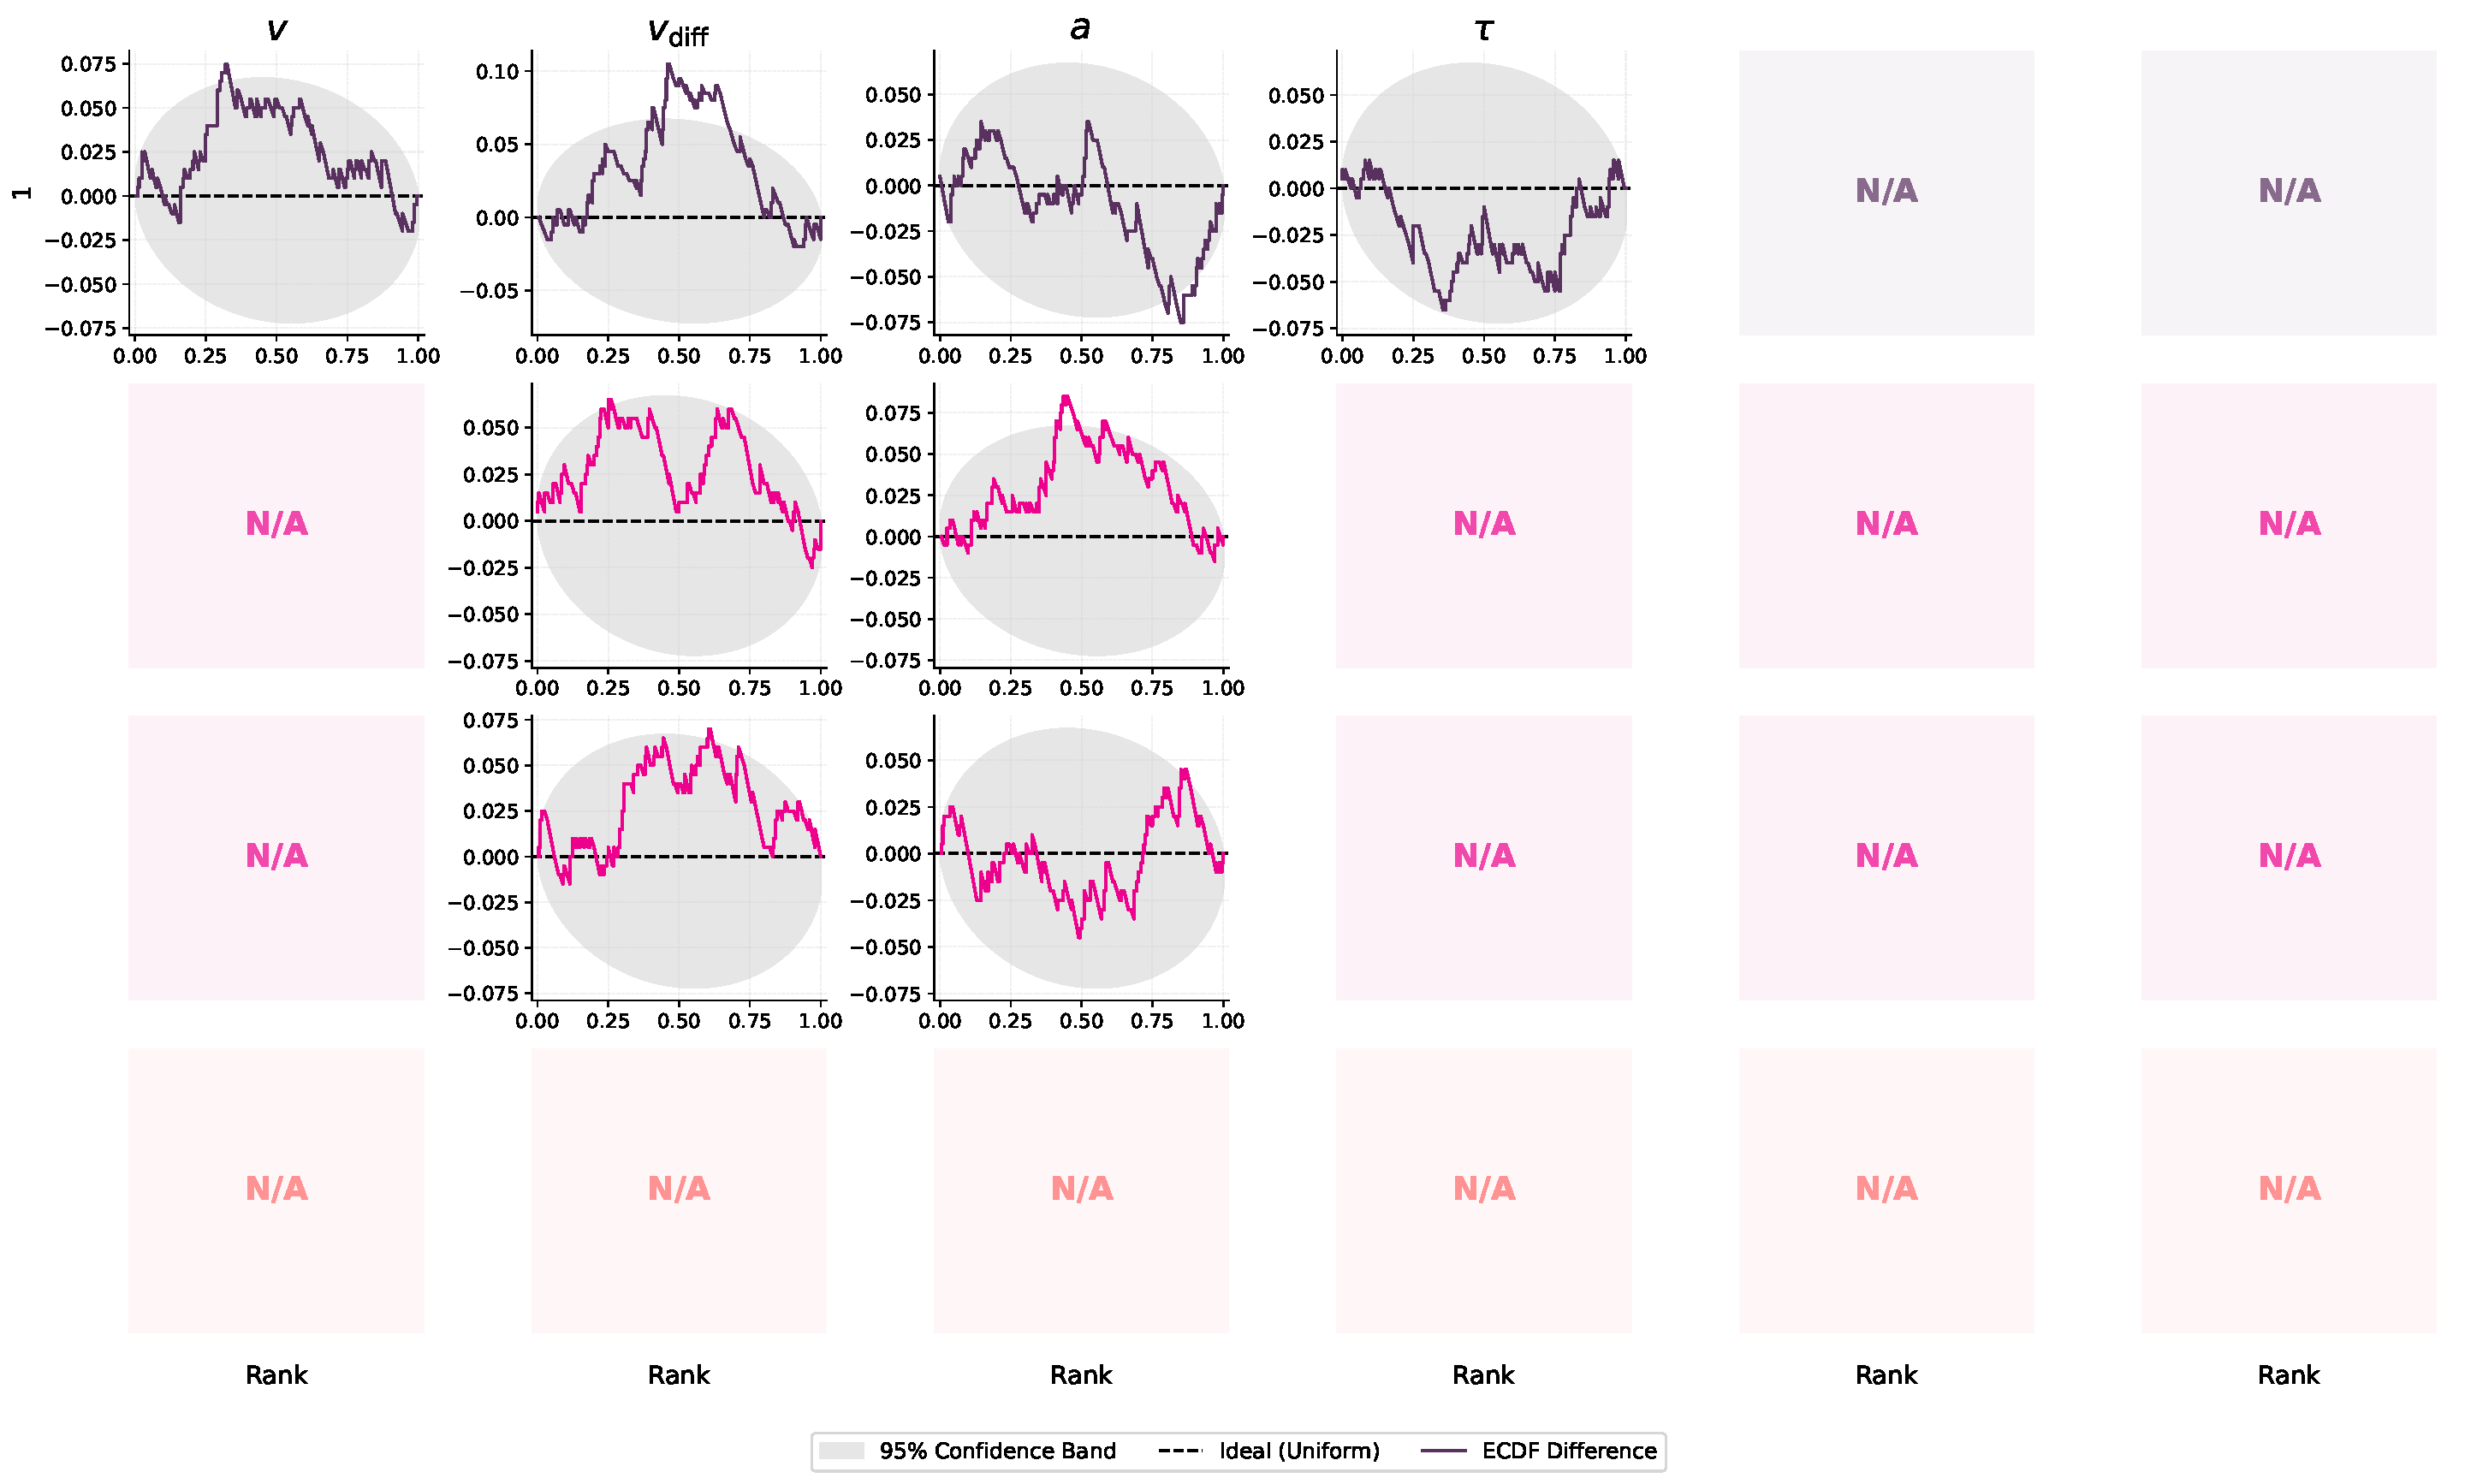
\includegraphics[width=0.99\linewidth]{figures/fm/rdm/fixed_regressed/rdm_family_fixed_regressed_fm_mixed_ecdf.pdf}
    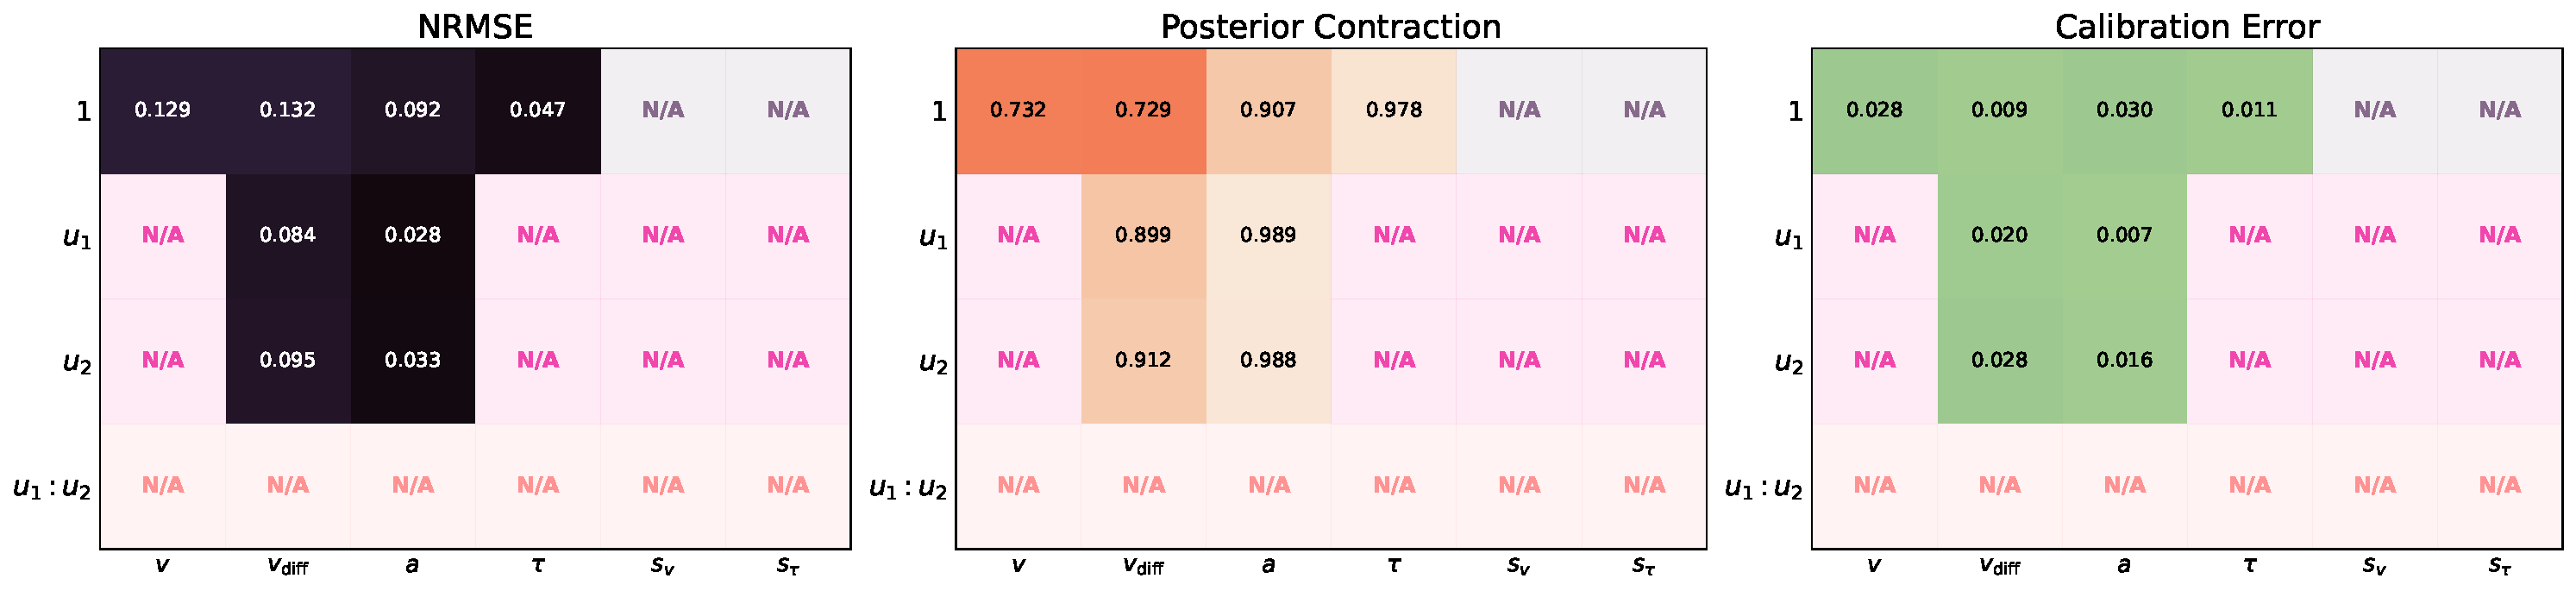
\includegraphics[width=0.99\linewidth]{figures/fm/rdm/fixed_regressed/rdm_family_fixed_regressed_fm_mixed_metrics.pdf}
    \caption{Parameter recovery (\emph{top}), calibration ECDF (\emph{middle}), and parameter-wise metrics (NRMSE, calibration error, and posterior contraction) for RDM model family (Case \textbf{fixed\_regressed}).}
    \label{fig:rdm-fm-fixed-regressed}
\end{figure}

\begin{figure}
    \centering
    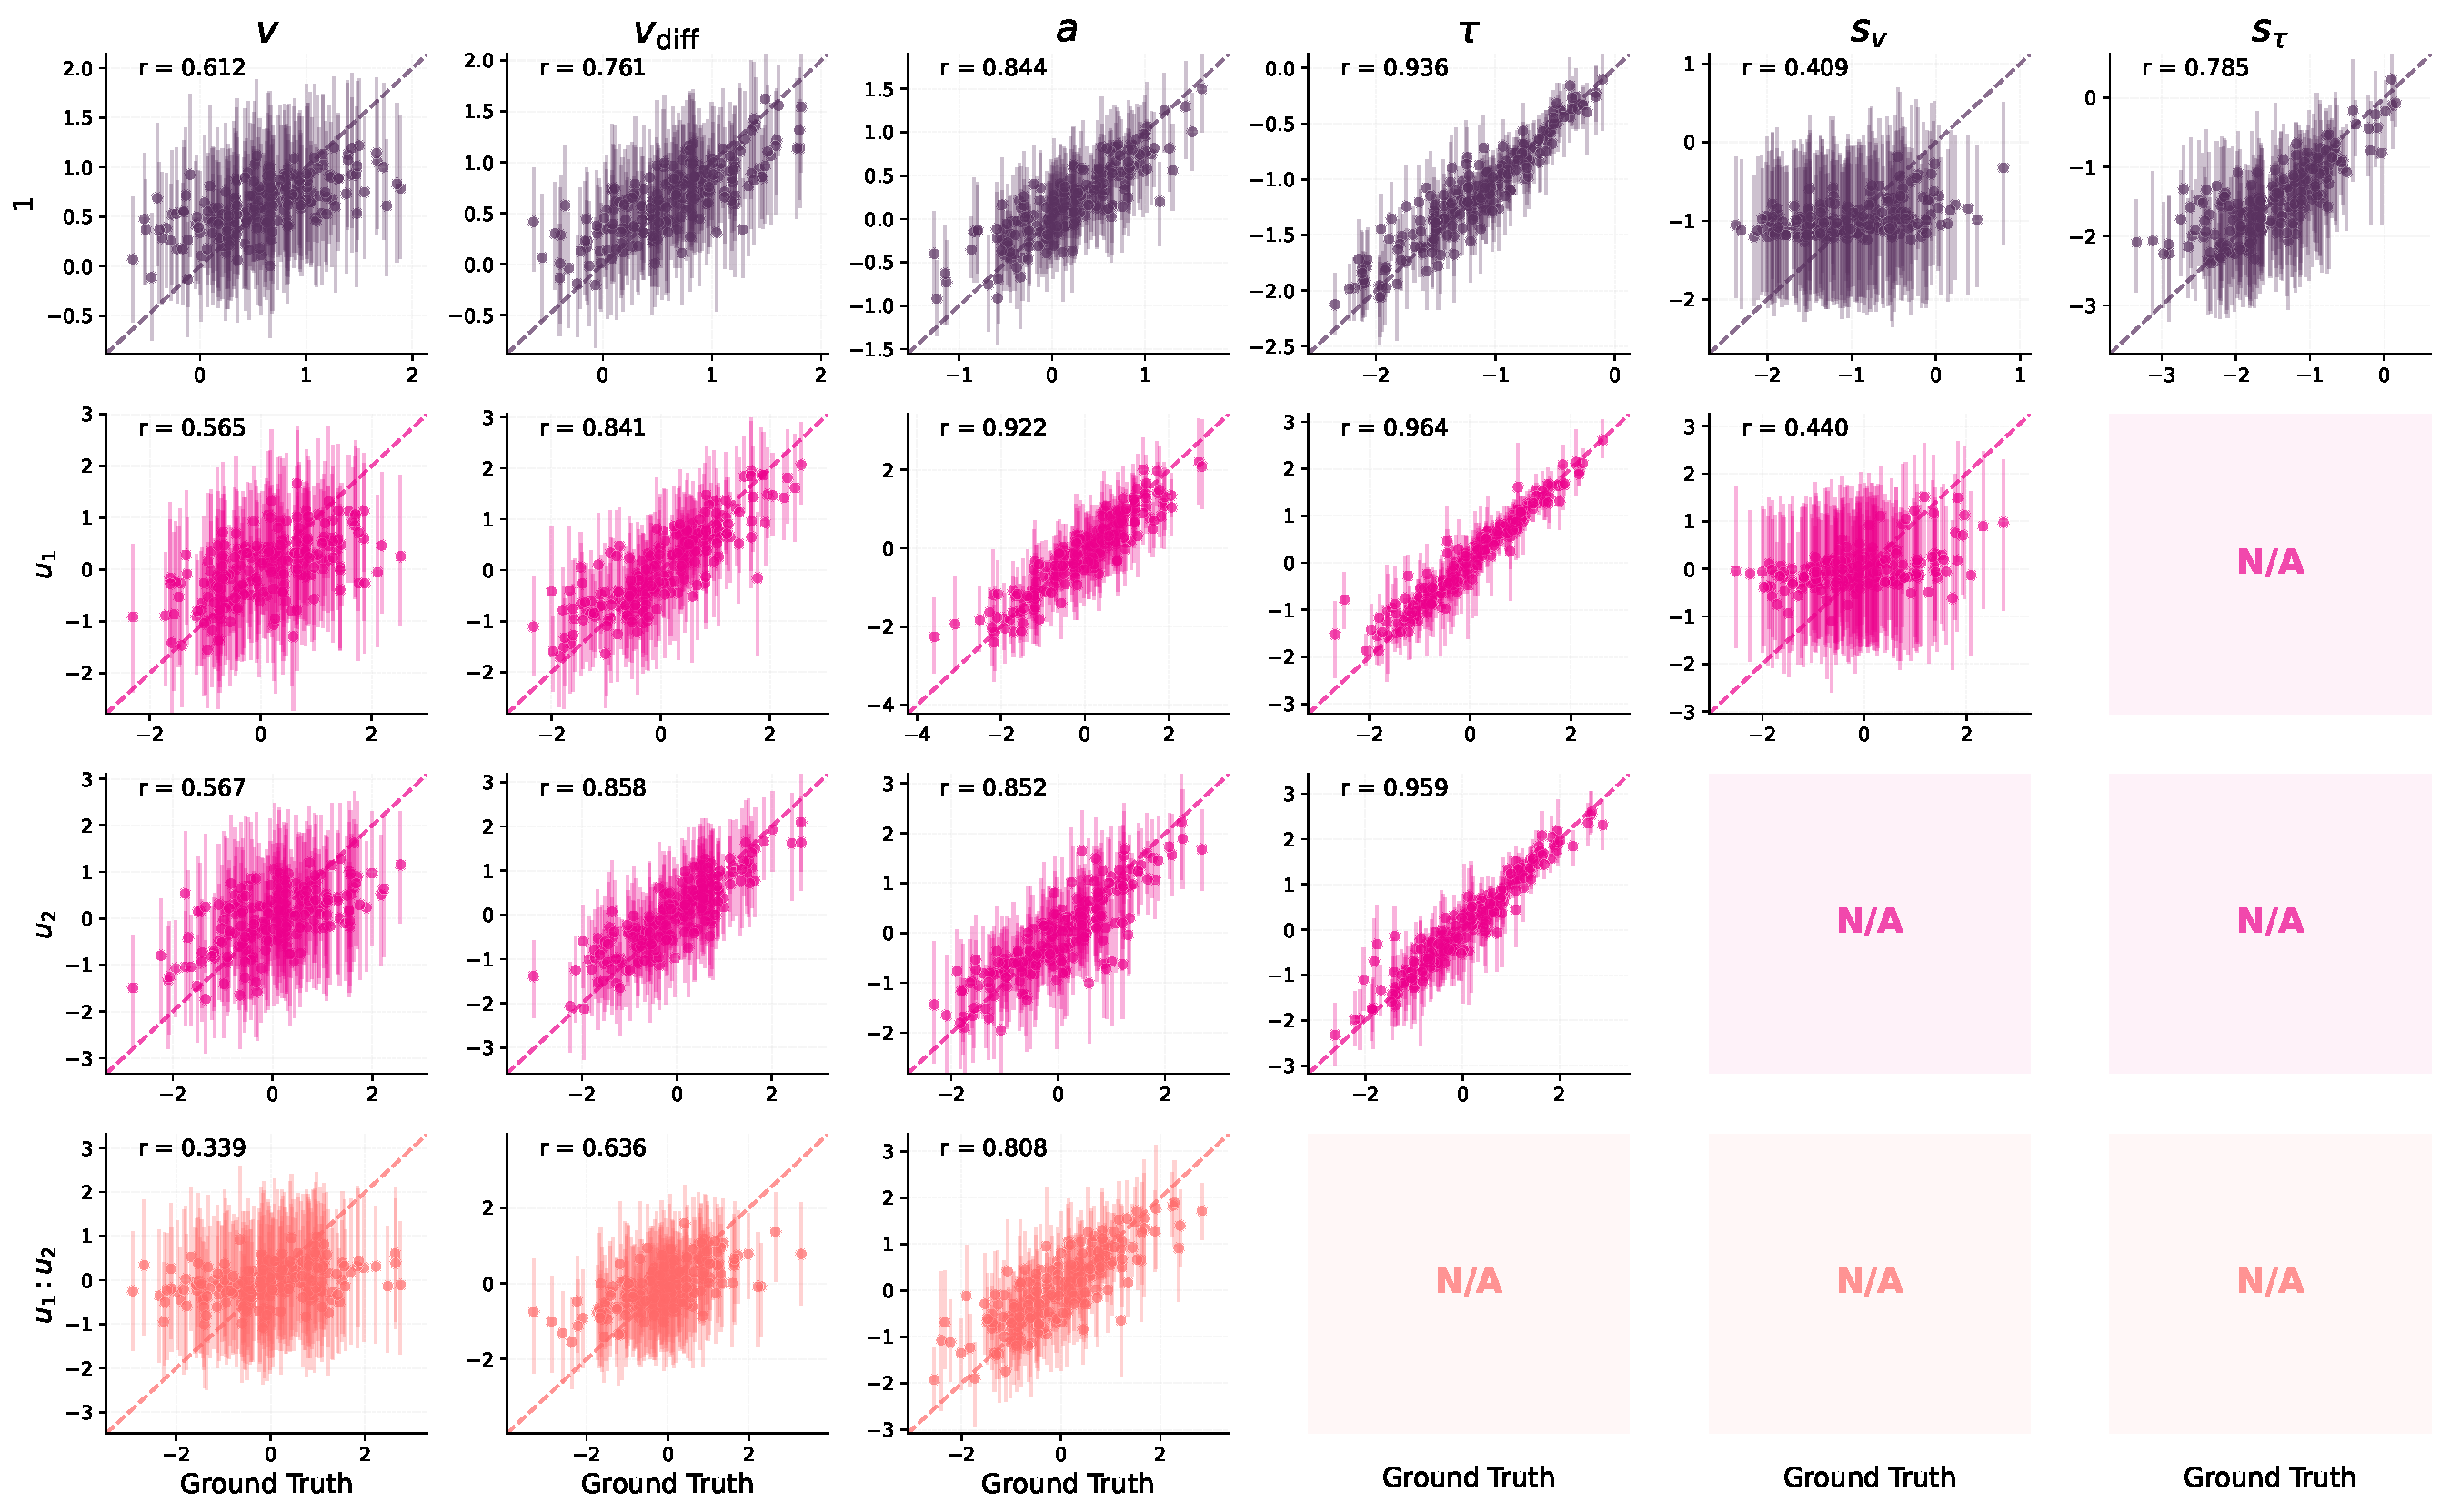
\includegraphics[width=0.99\linewidth]{figures/fm/rdm/interaction/rdm_family_interaction_fm_mixed_recovery.pdf}
    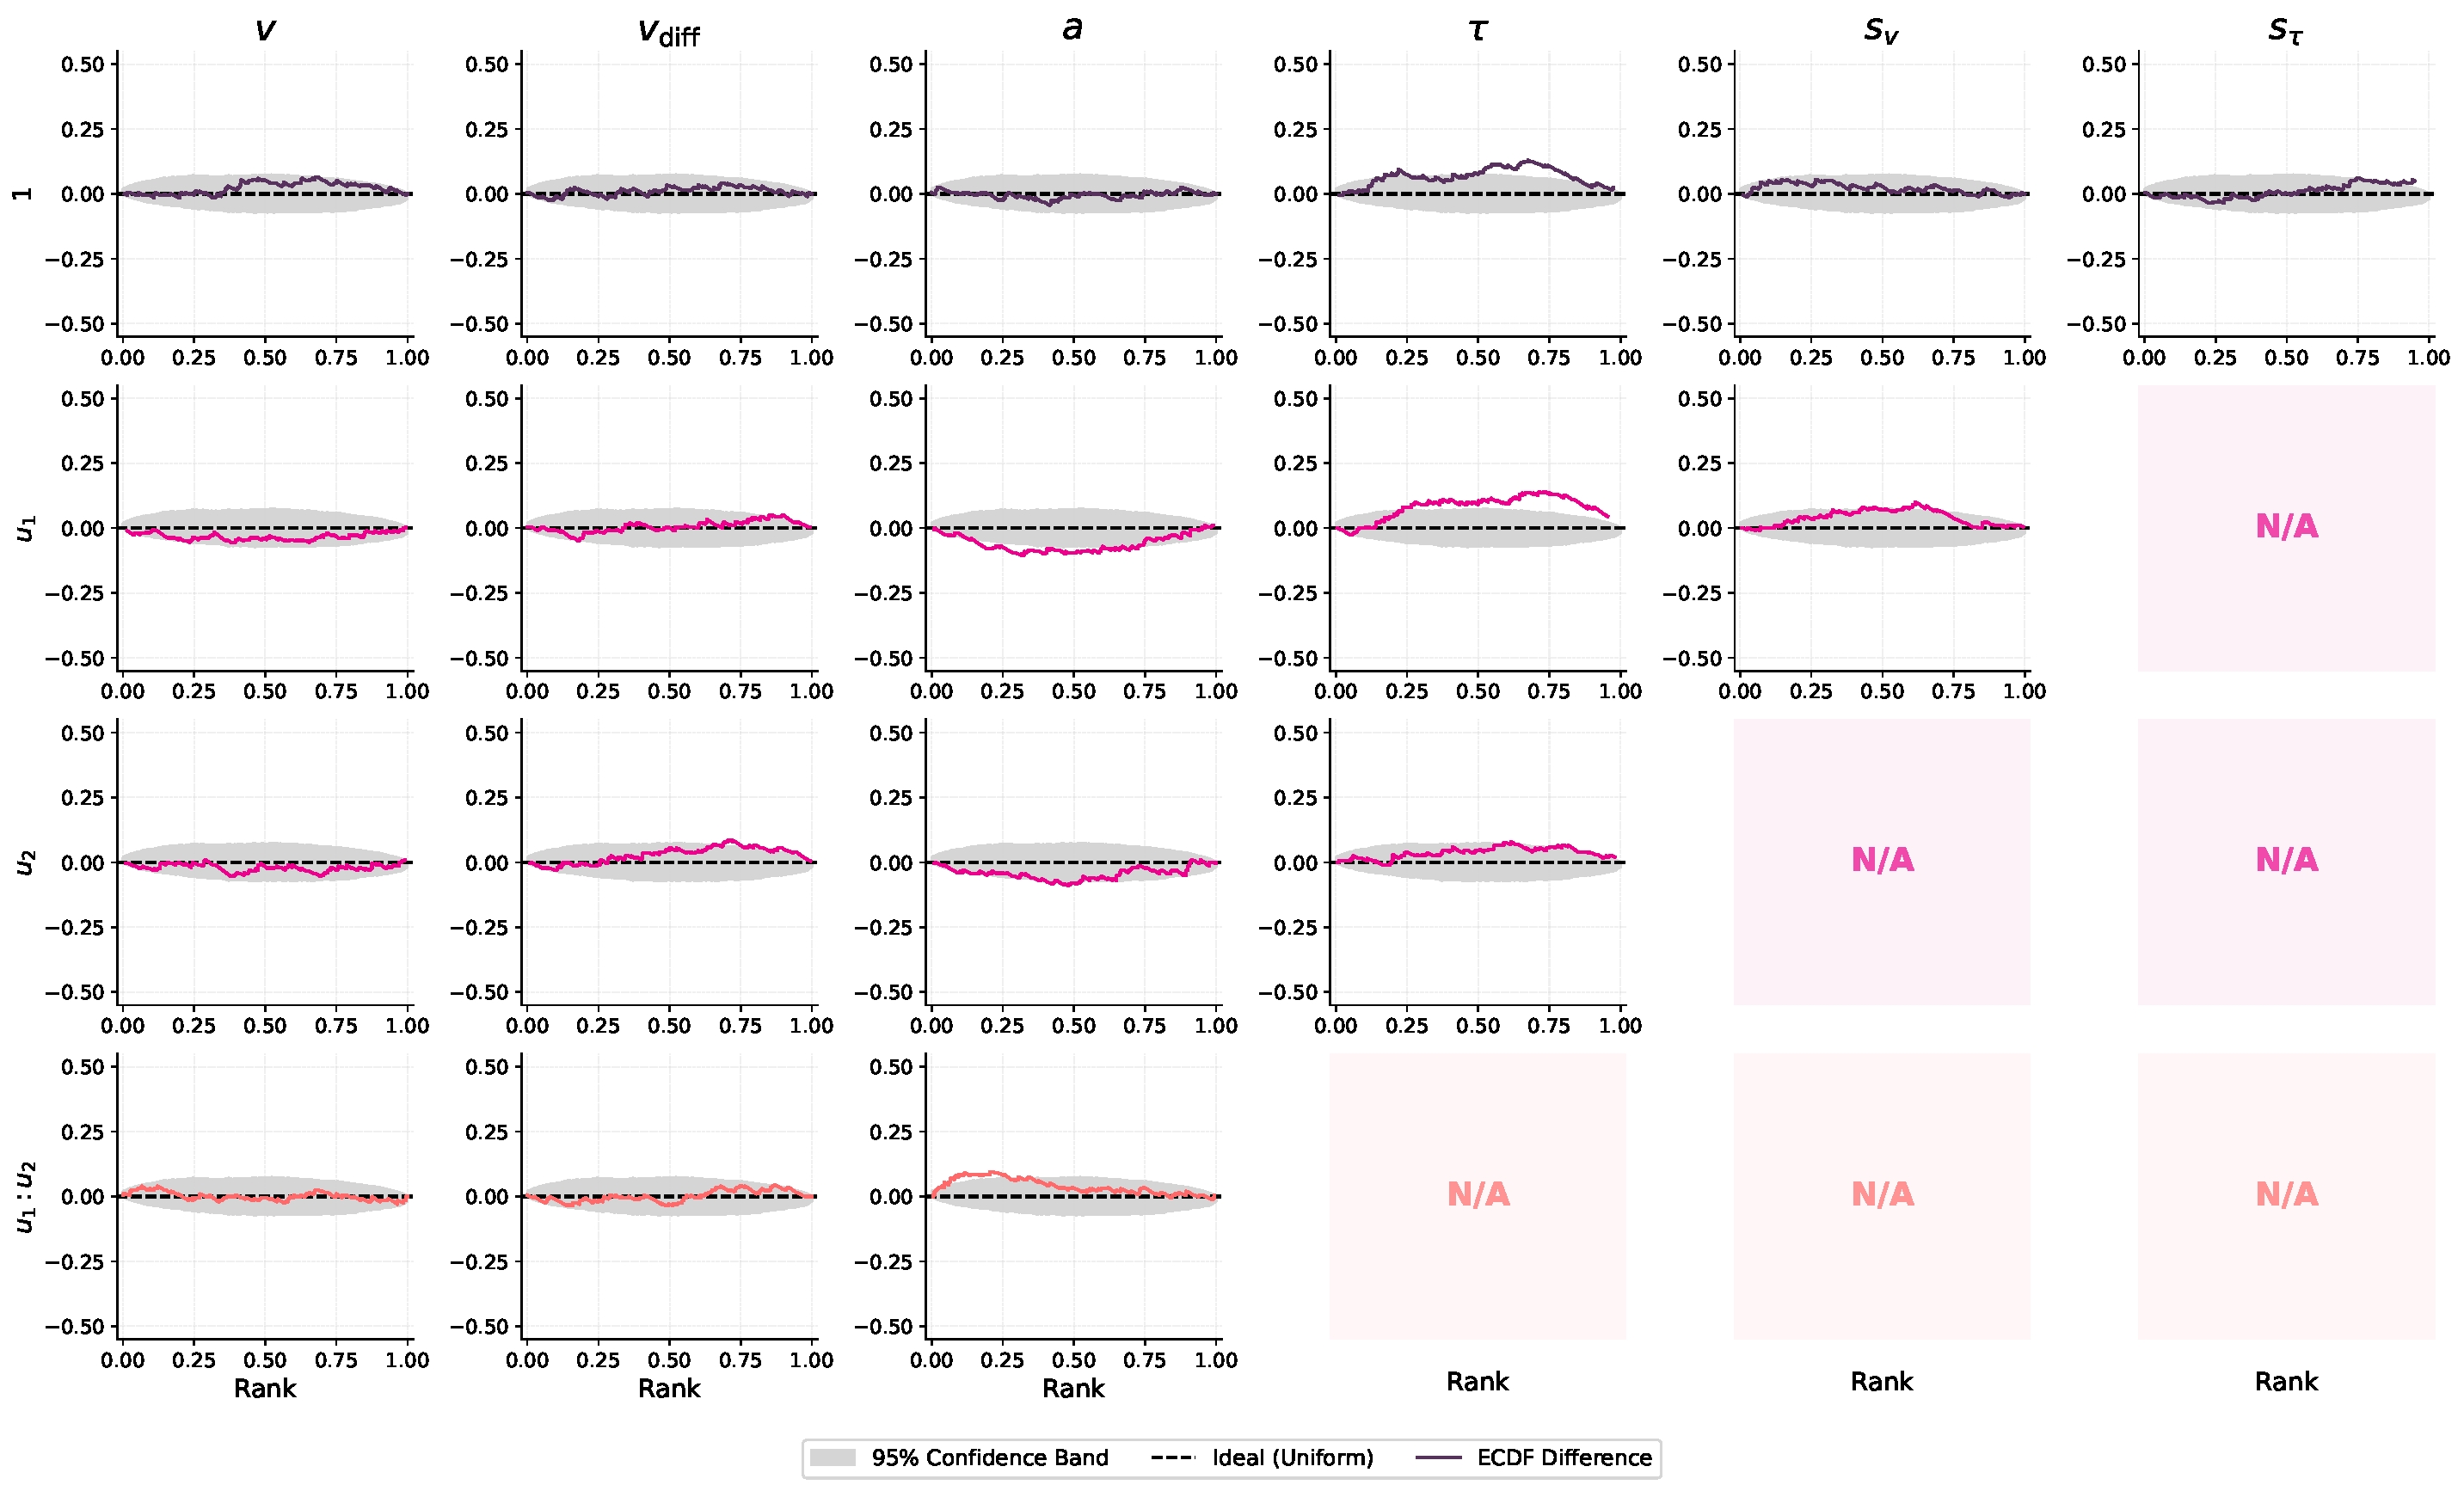
\includegraphics[width=0.99\linewidth]{figures/fm/rdm/interaction/rdm_family_interaction_fm_mixed_ecdf.pdf}
    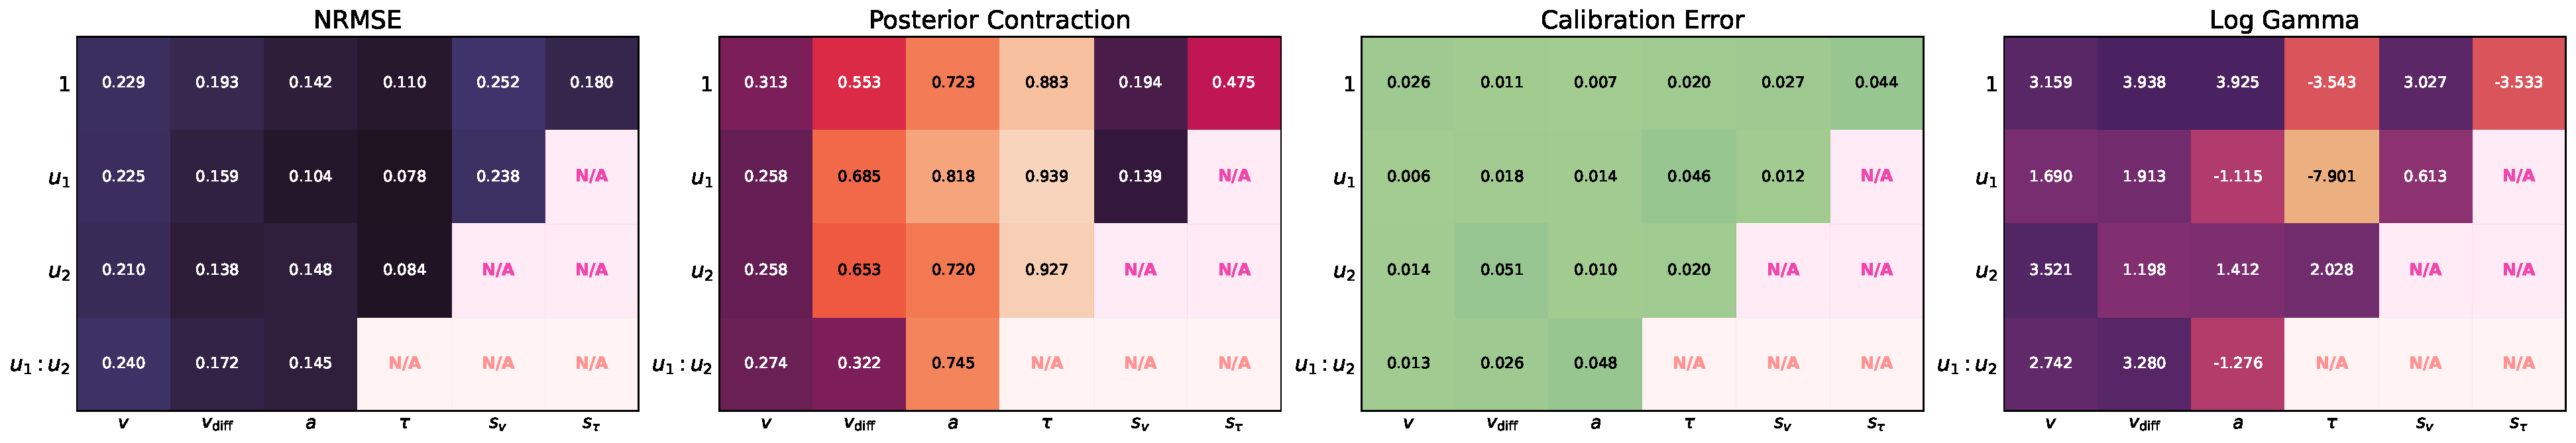
\includegraphics[width=0.99\linewidth]{figures/fm/rdm/interaction/rdm_family_interaction_fm_mixed_metrics.pdf}
    \caption{Parameter recovery (\emph{top}), calibration ECDF (\emph{middle}), and parameter-wise metrics (NRMSE, calibration error, and posterior contraction) for RDM model family (Case \textbf{interaction}).}
    \label{fig:rdm-fm-interaction}
\end{figure}

% ========================================
% CDM BASELINE (bf)
% ========================================

\begin{figure}
    \centering
    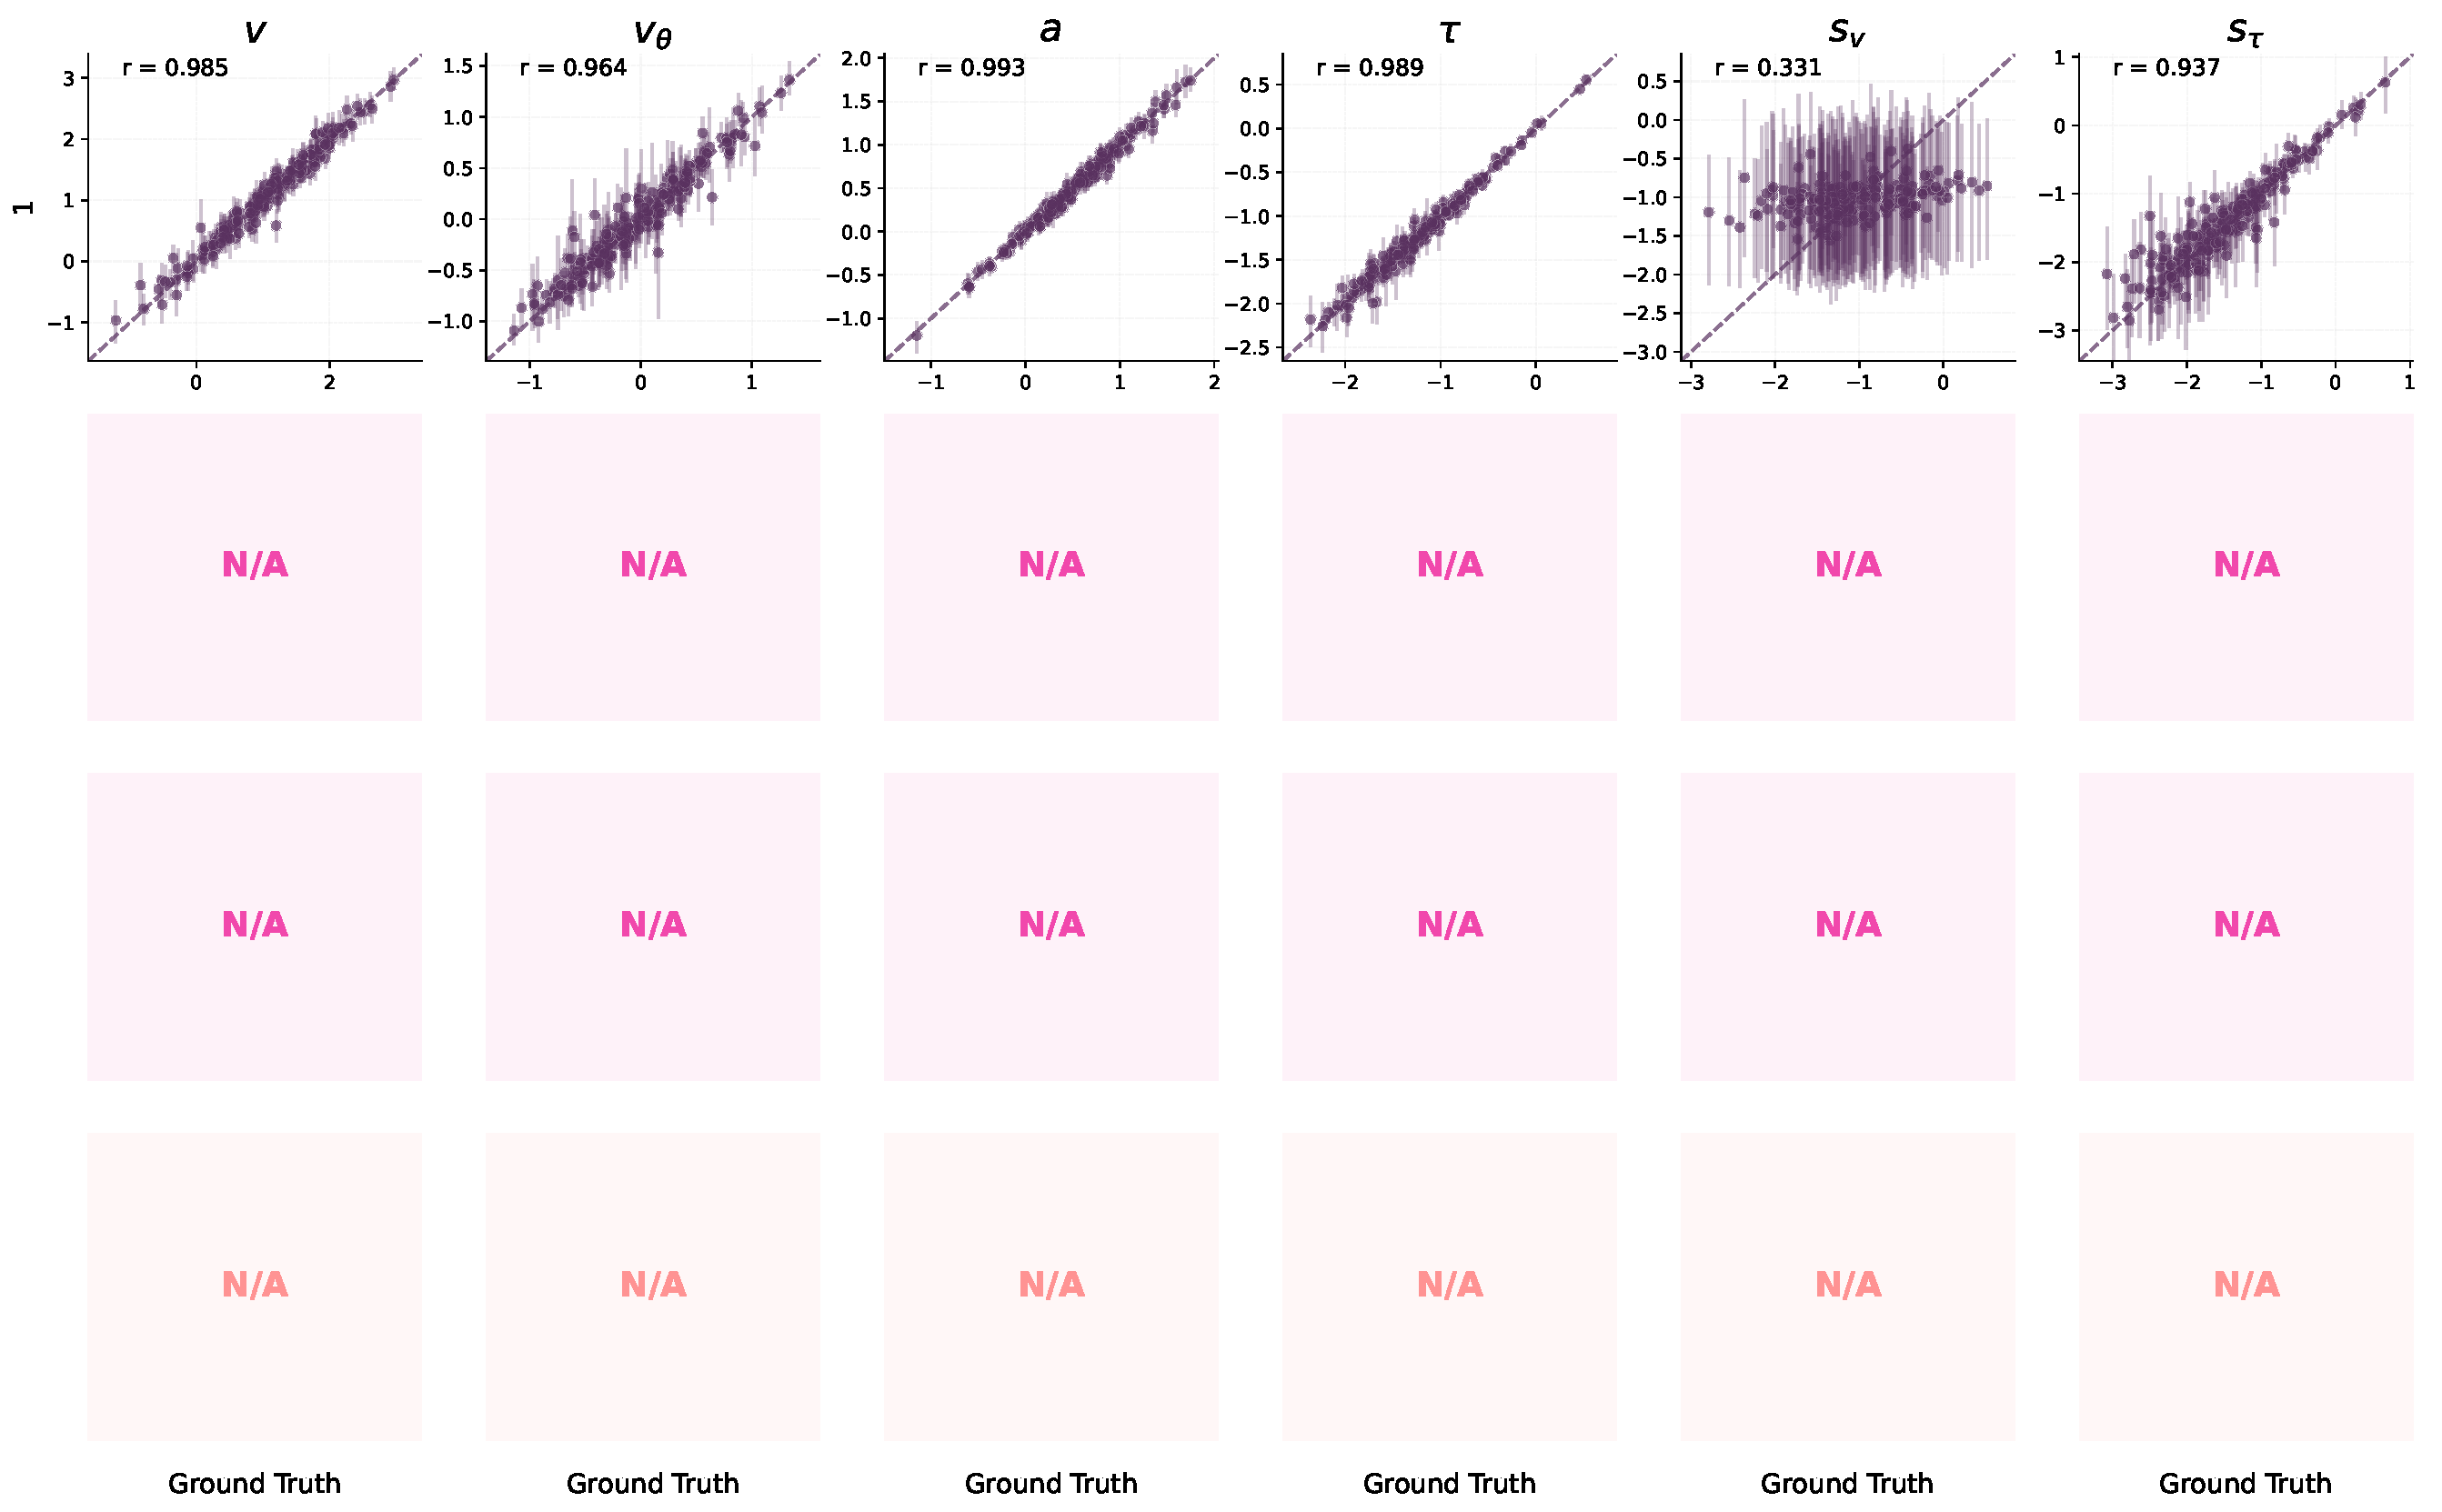
\includegraphics[width=0.99\linewidth]{figures/bf/cdm/intercept_only/cdm_family_intercept_only_bf_recovery.pdf}
    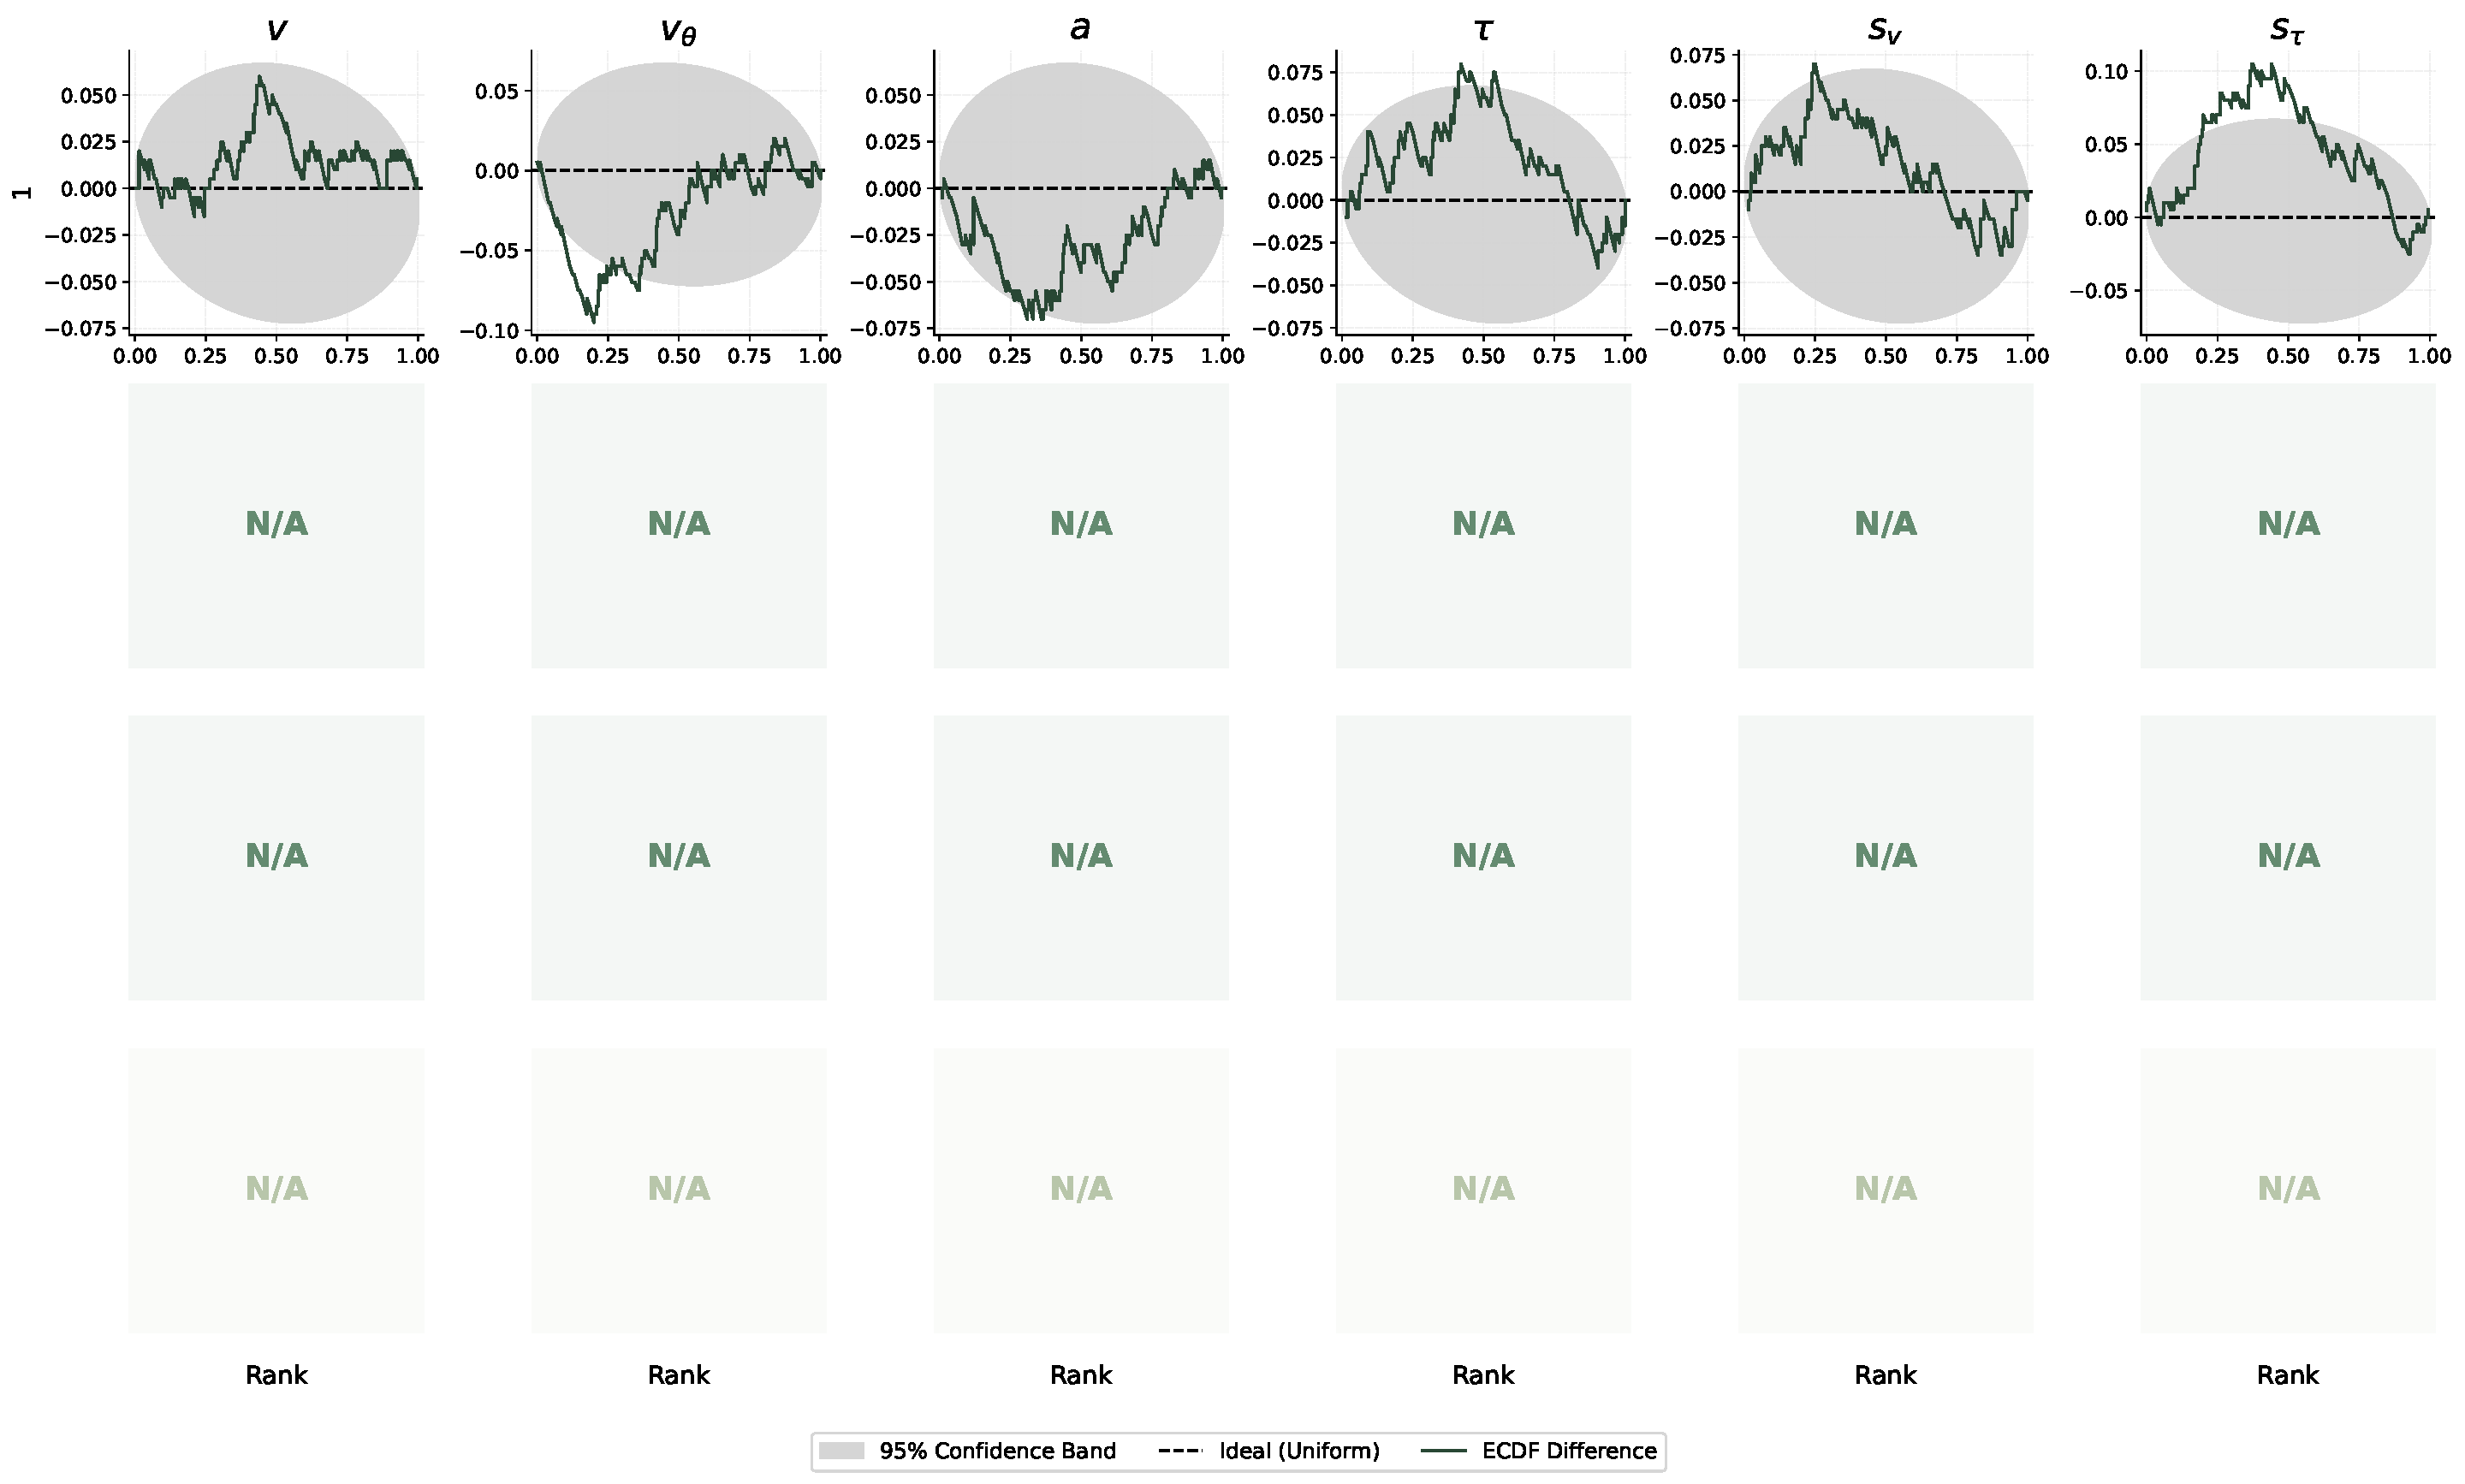
\includegraphics[width=0.99\linewidth]{figures/bf/cdm/intercept_only/cdm_family_intercept_only_bf_ecdf.pdf}
    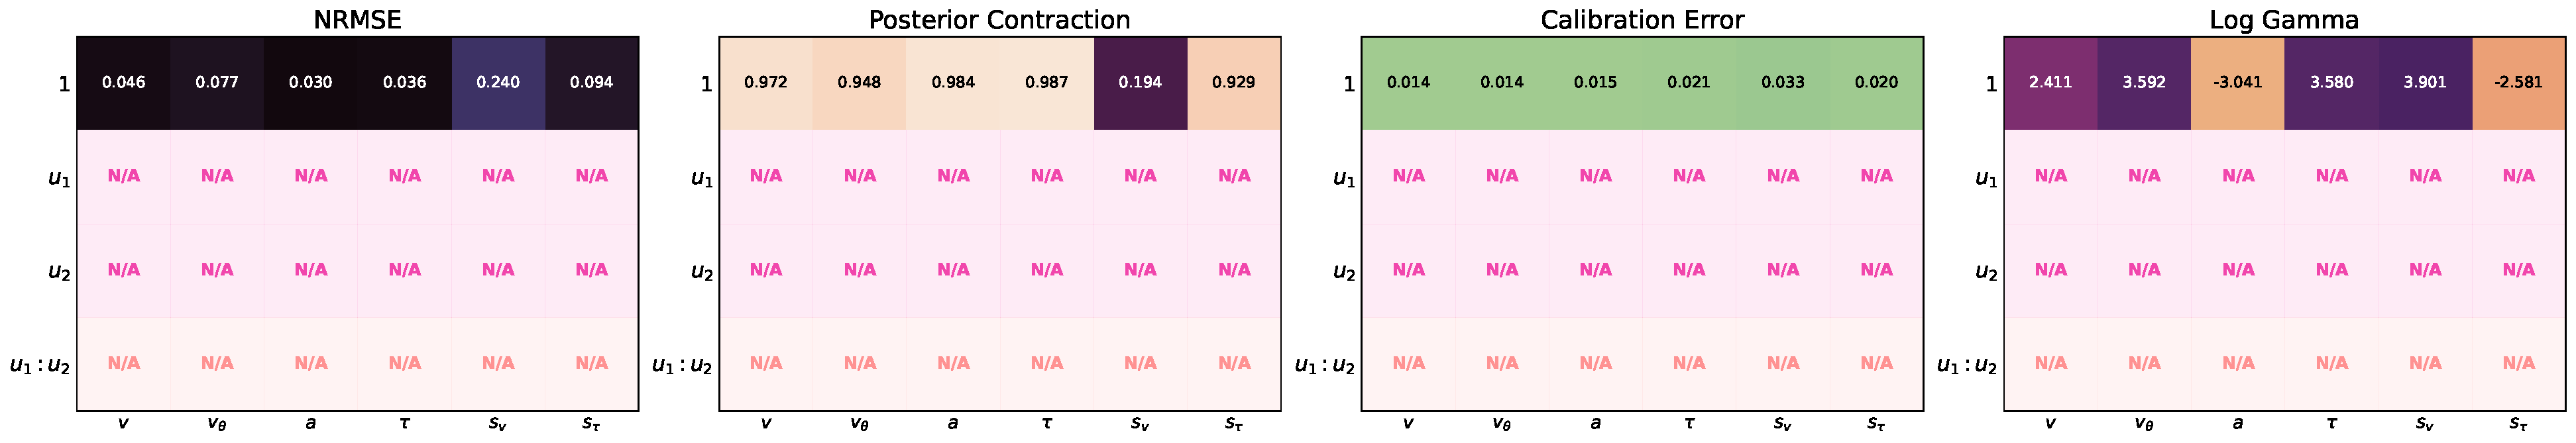
\includegraphics[width=0.99\linewidth]{figures/bf/cdm/intercept_only/cdm_family_intercept_only_bf_metrics.pdf}
    \caption{Parameter recovery (\emph{top}), calibration ECDF (\emph{middle}), and parameter-wise metrics (NRMSE, calibration error, and posterior contraction) for CDM baseline (Case \textbf{intercept\_only}).}
    \label{fig:cdm-bf-intercept-only}
\end{figure}

\begin{figure}
    \centering
    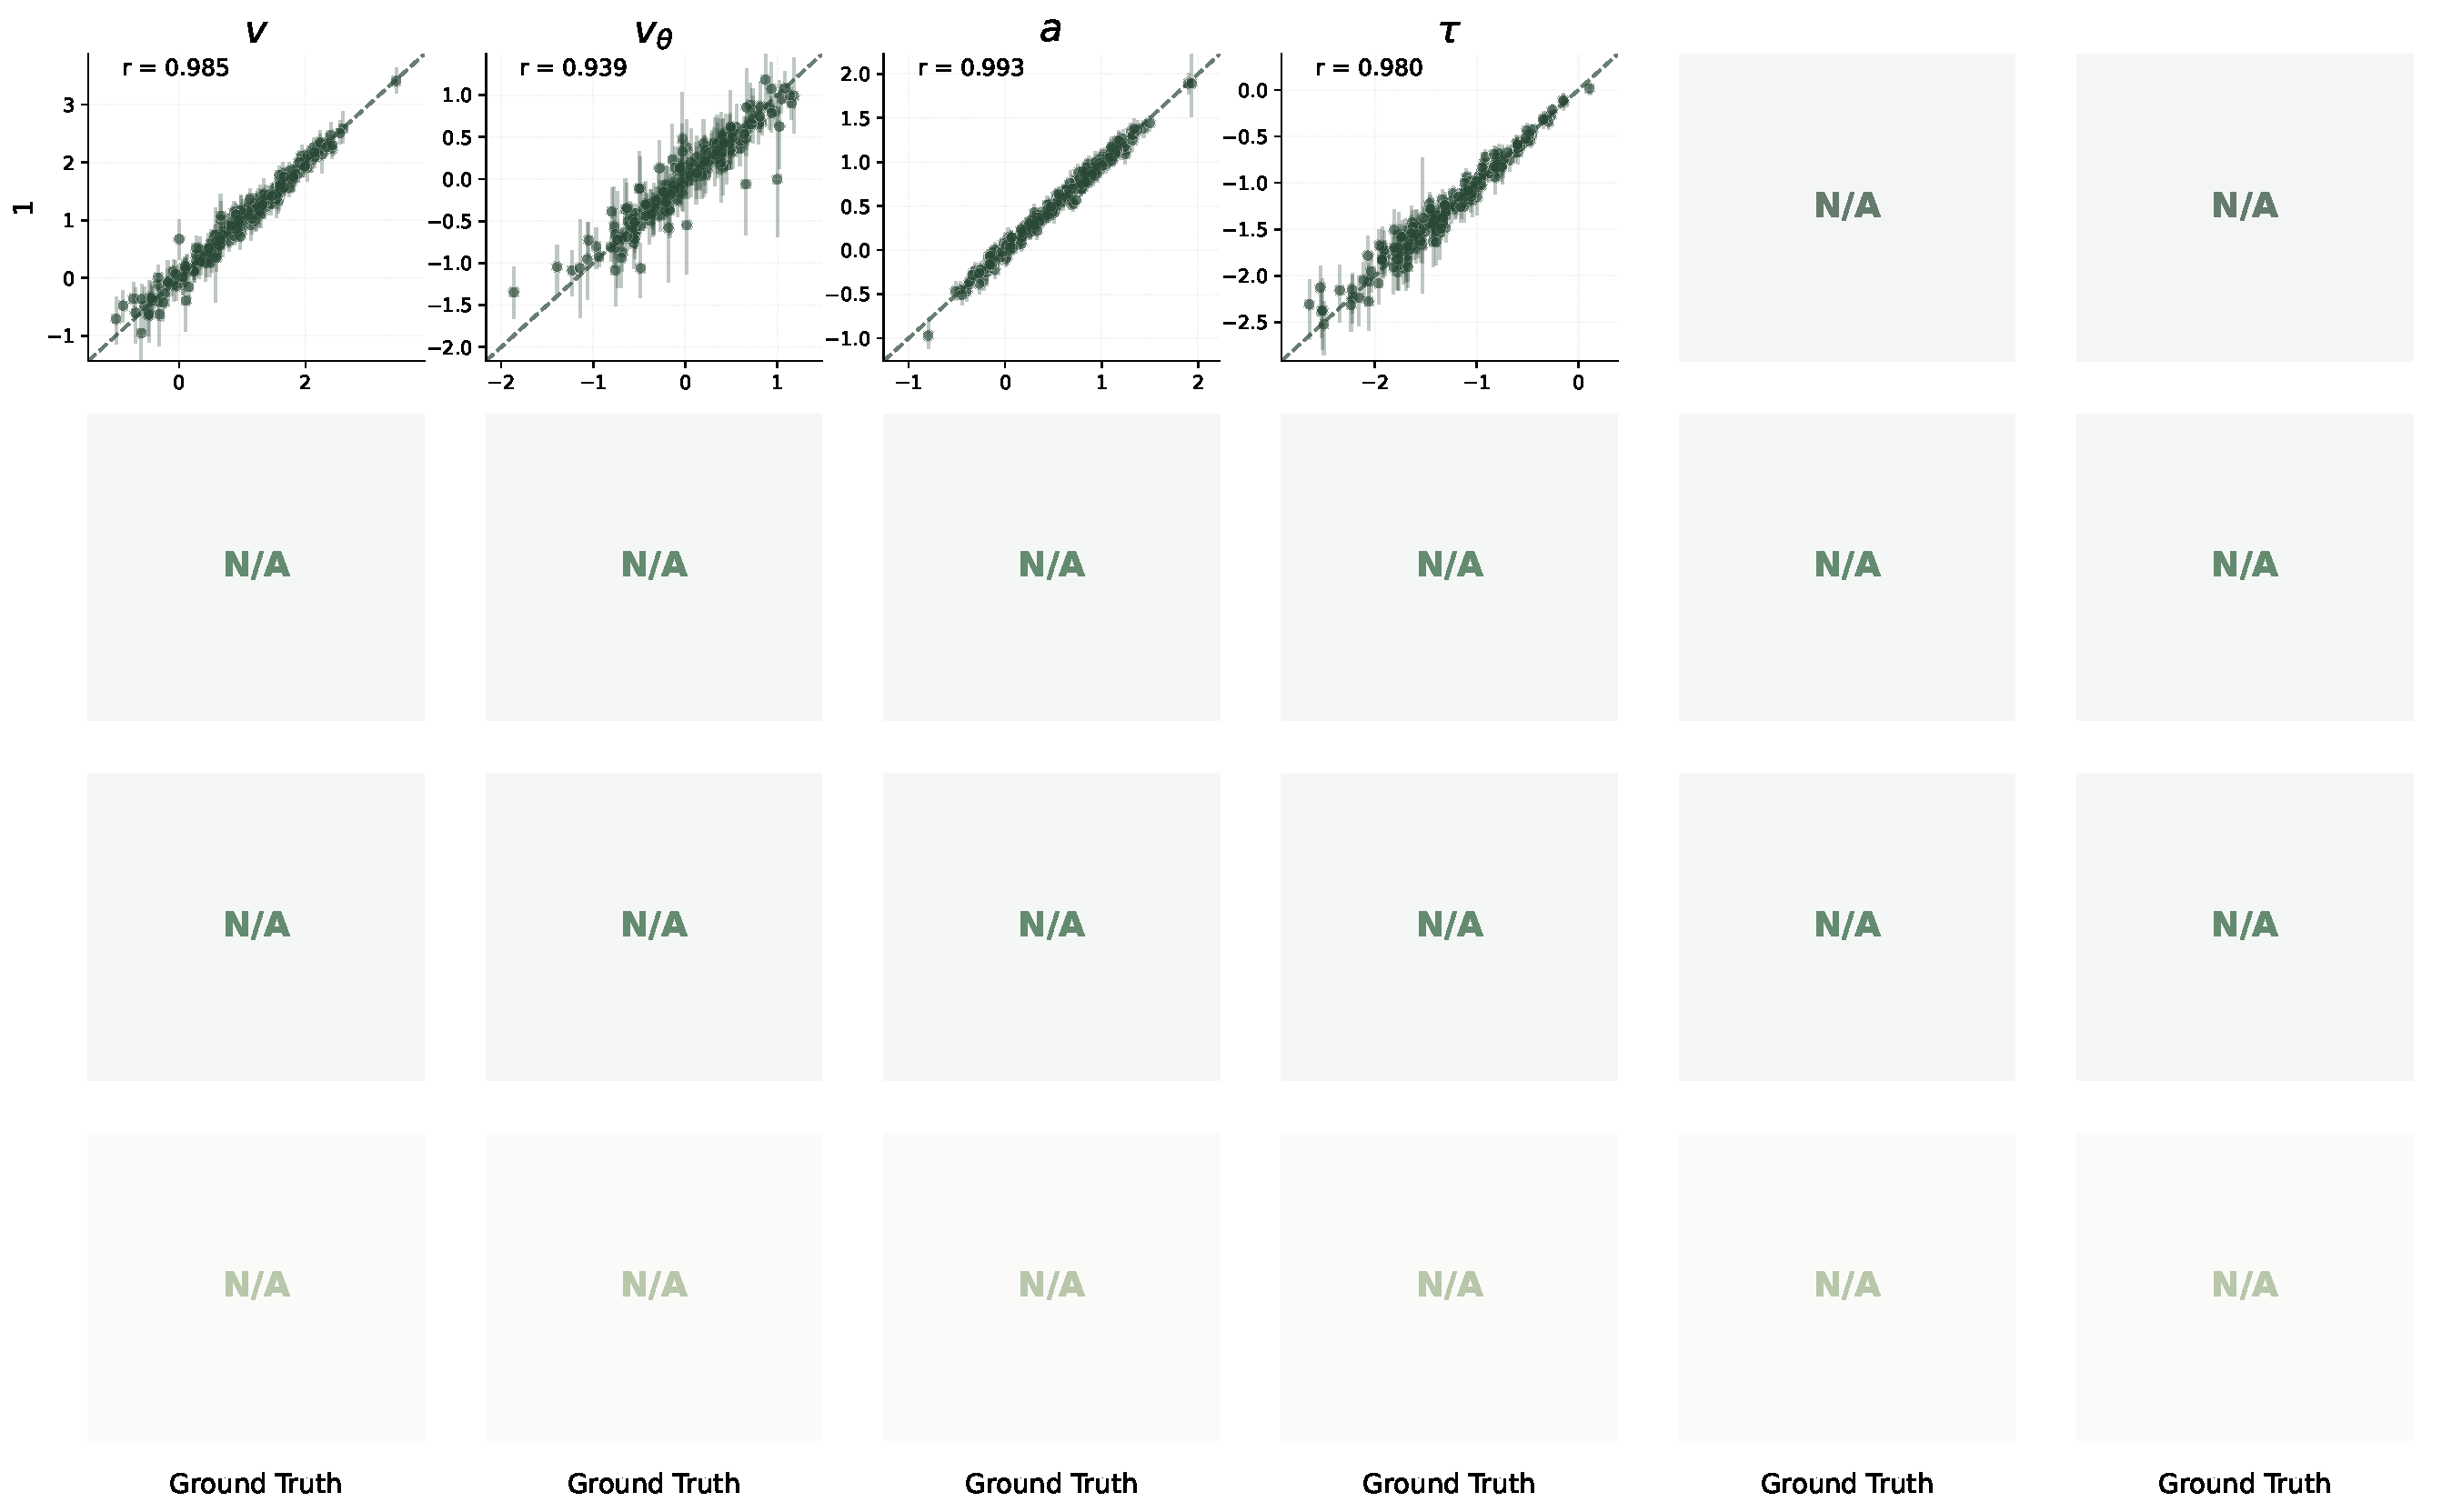
\includegraphics[width=0.99\linewidth]{figures/bf/cdm/fixed/cdm_family_fixed_bf_recovery.pdf}
    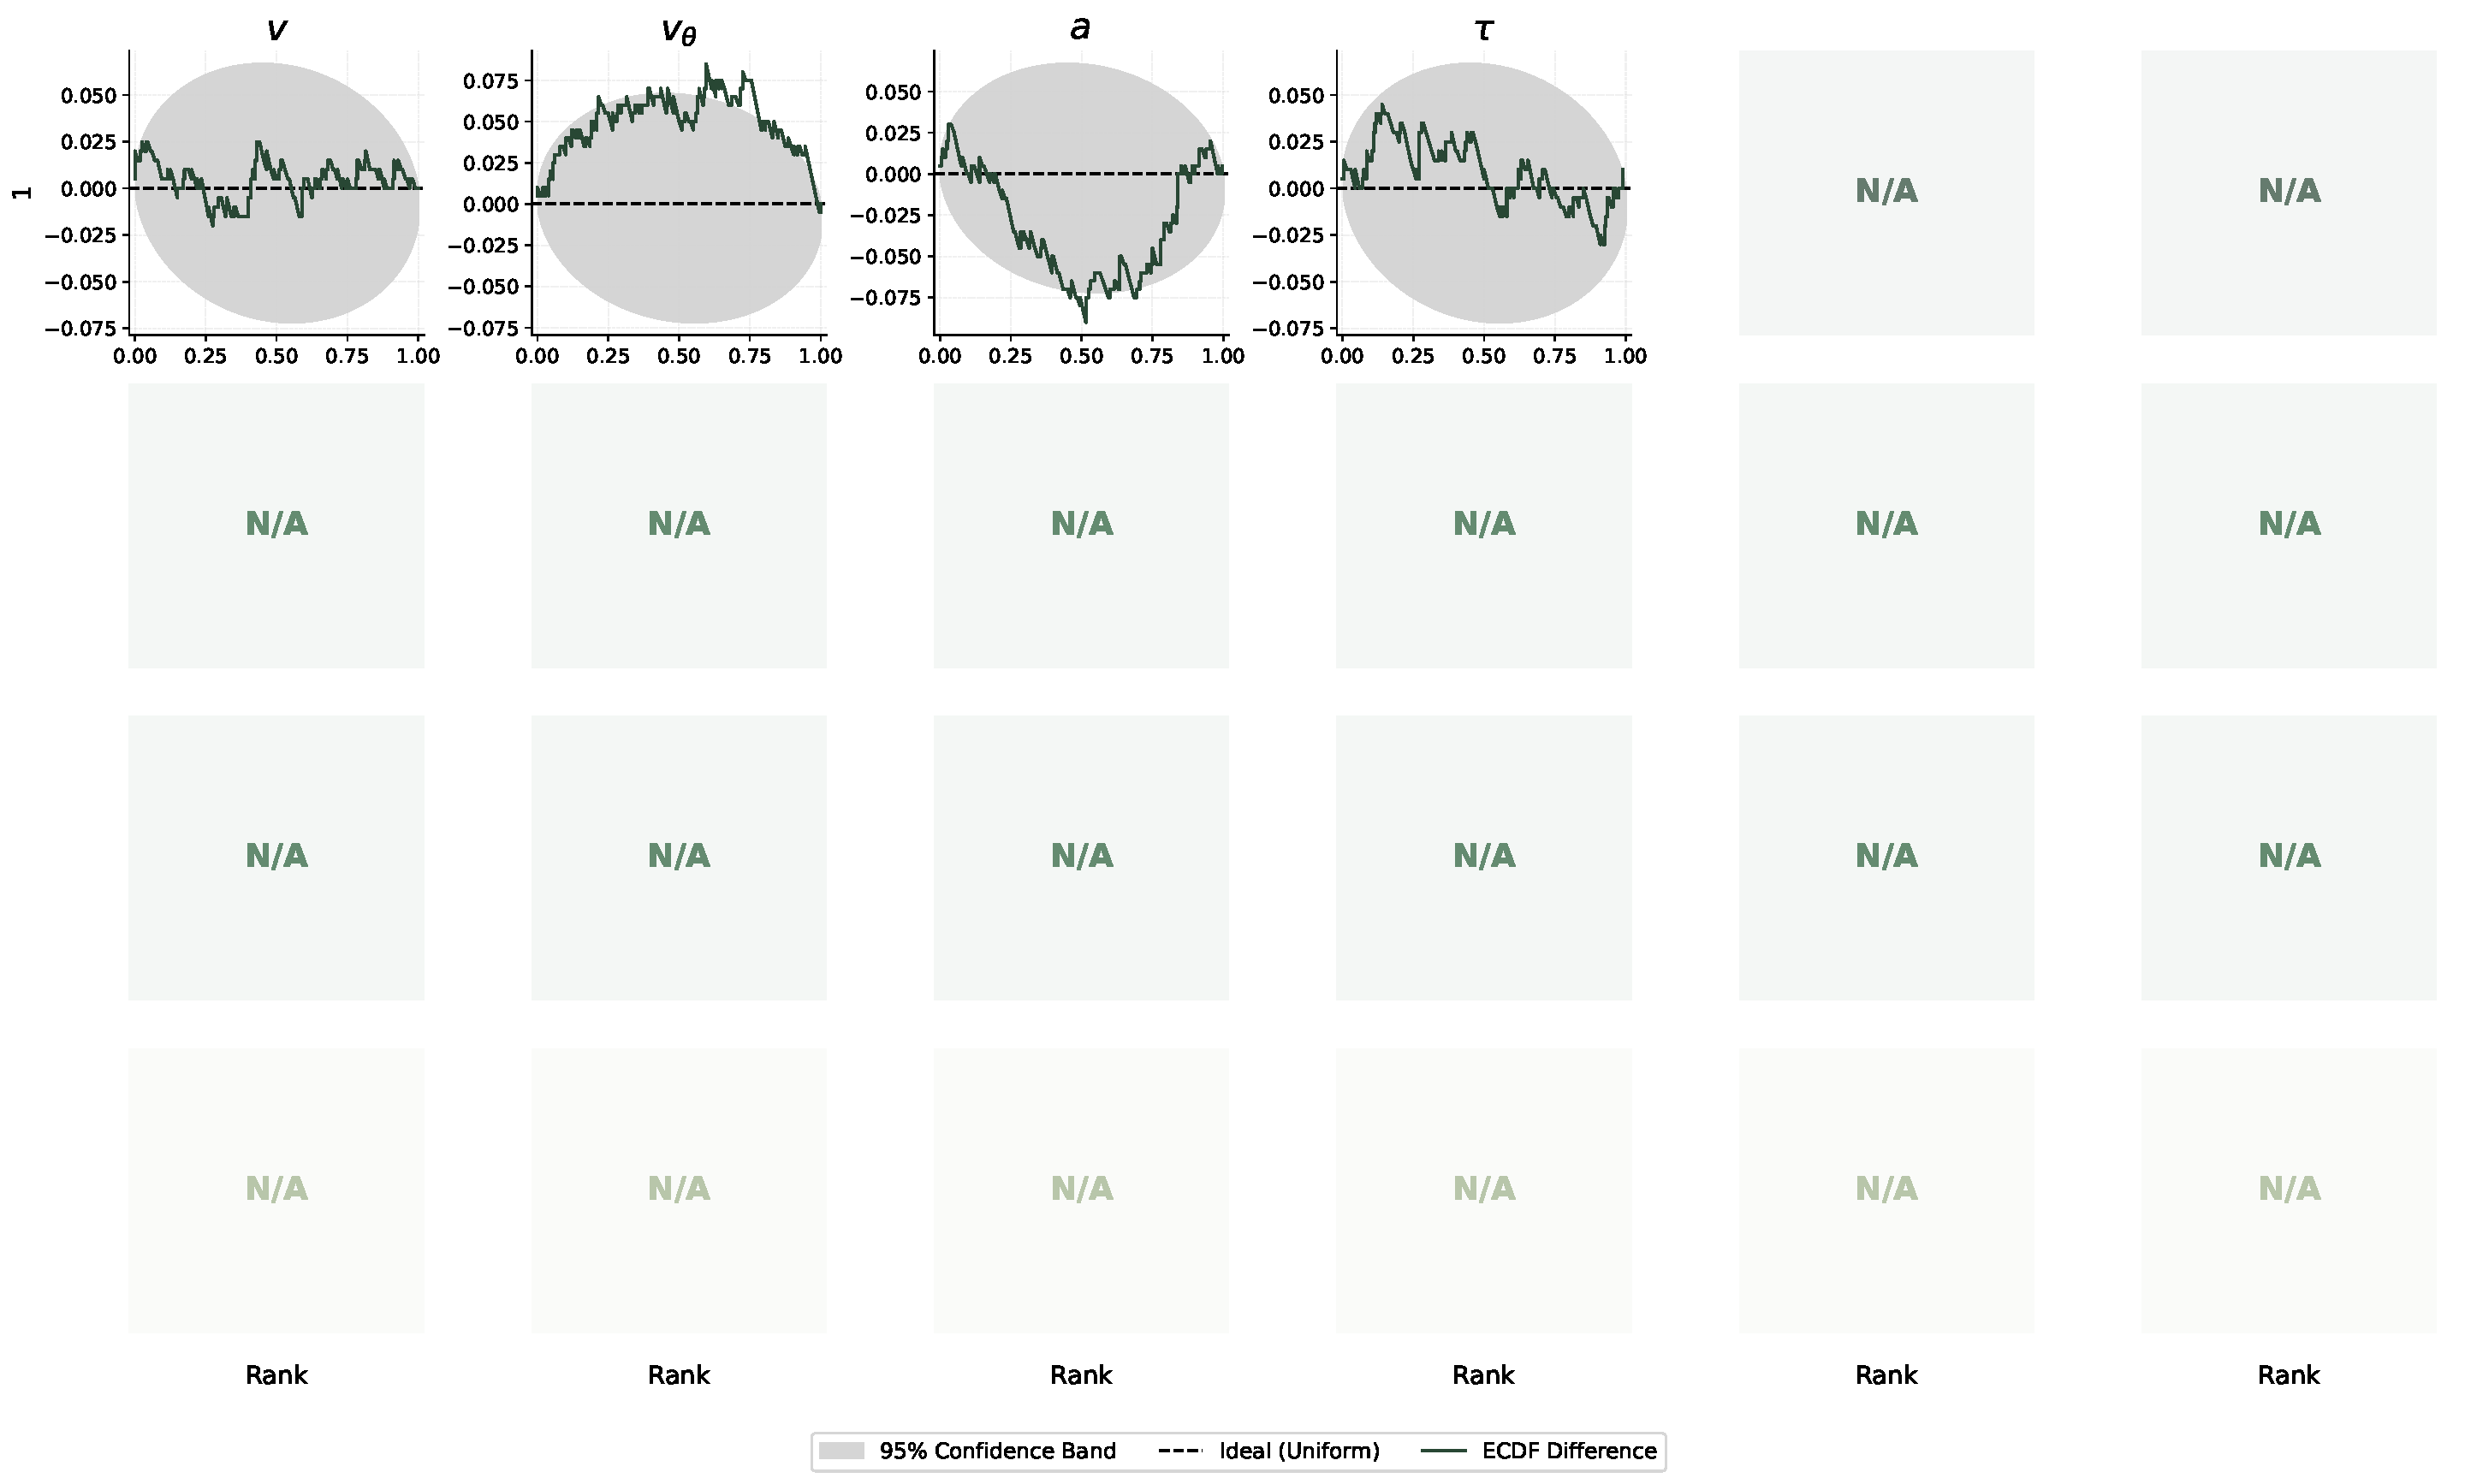
\includegraphics[width=0.99\linewidth]{figures/bf/cdm/fixed/cdm_family_fixed_bf_ecdf.pdf}
    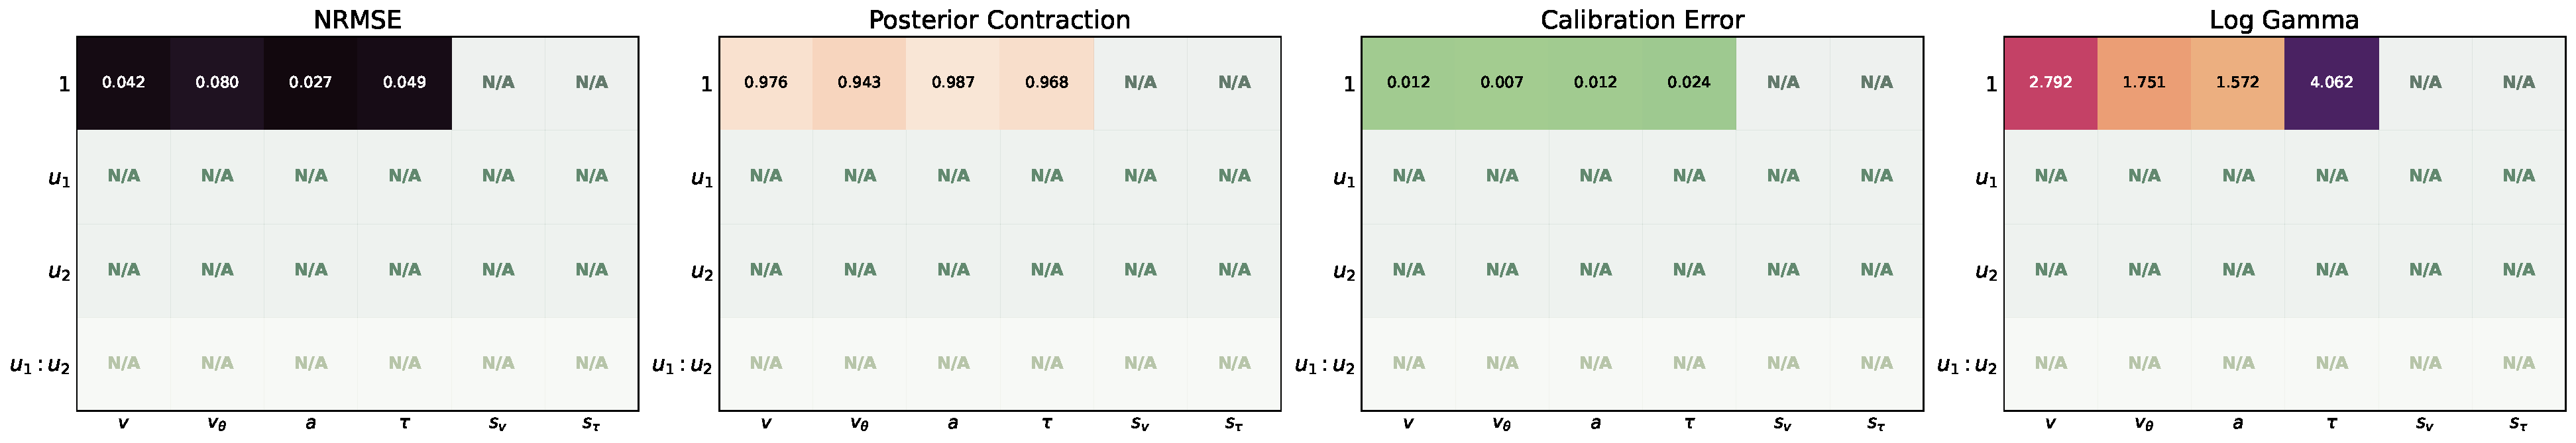
\includegraphics[width=0.99\linewidth]{figures/bf/cdm/fixed/cdm_family_fixed_bf_metrics.pdf}
    \caption{Parameter recovery (\emph{top}), calibration ECDF (\emph{middle}), and parameter-wise metrics (NRMSE, calibration error, and posterior contraction) for CDM baseline (Case \textbf{fixed}).}
    \label{fig:cdm-bf-fixed}
\end{figure}

\begin{figure}
    \centering
    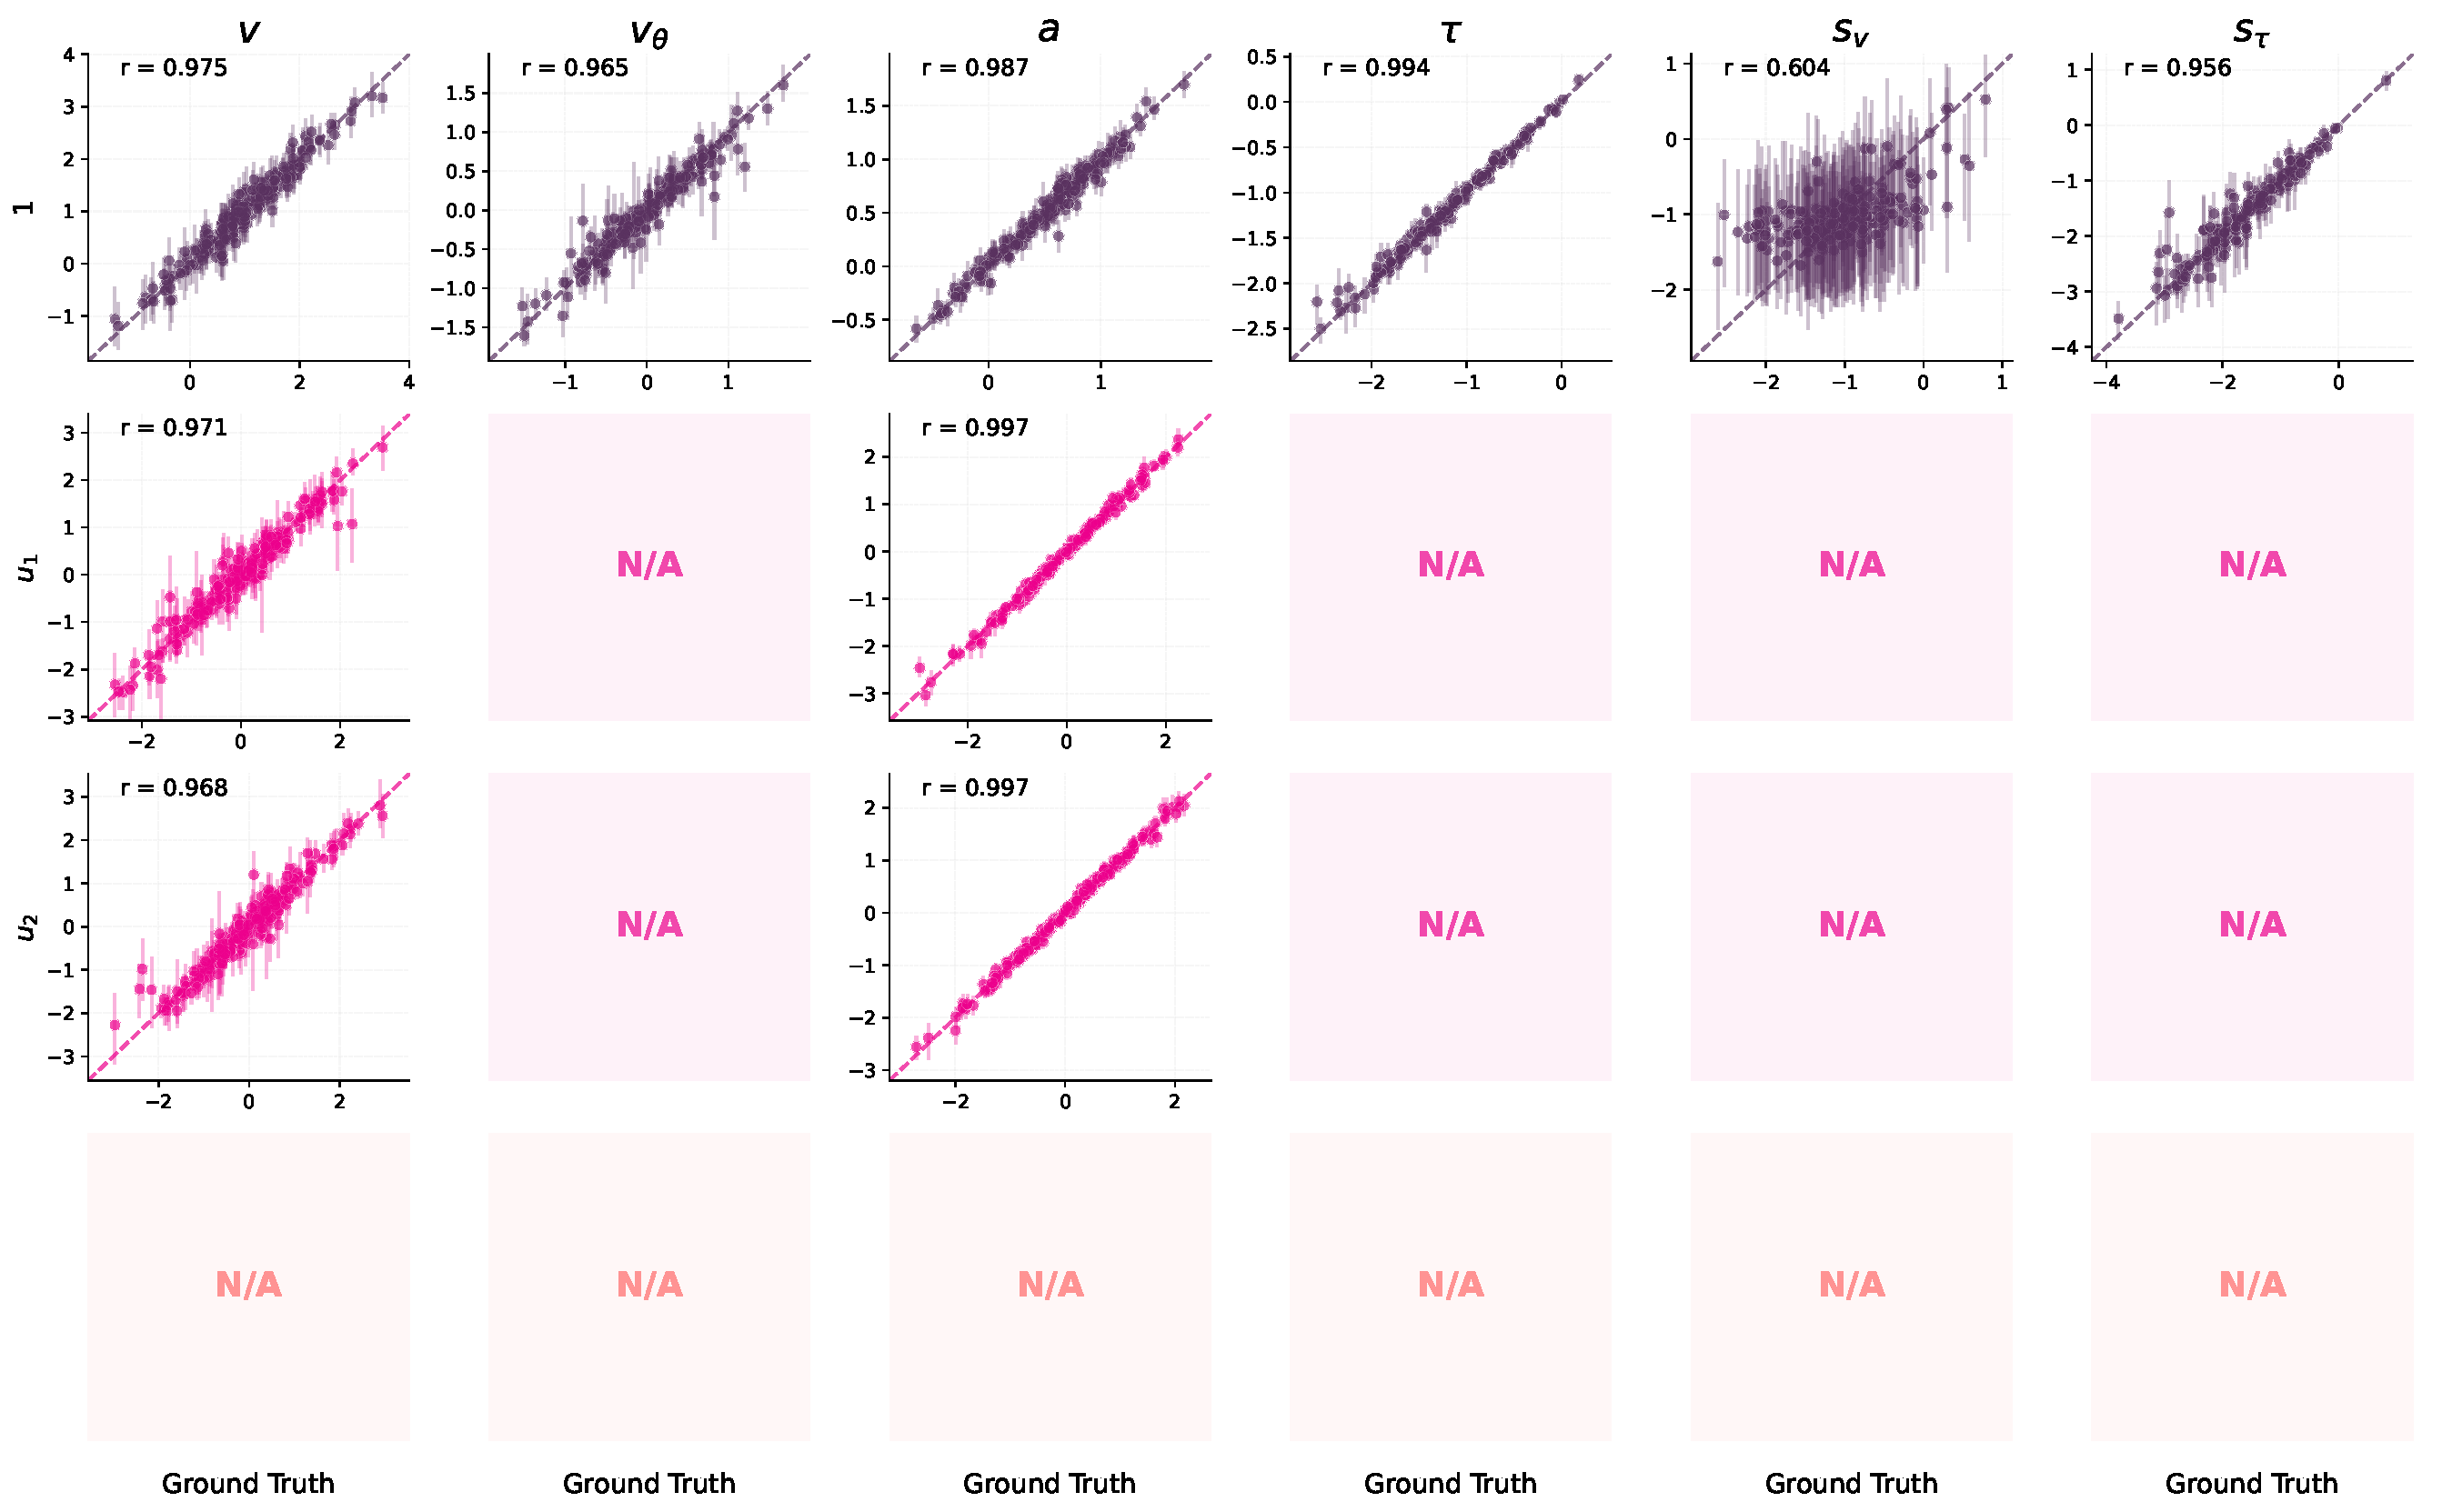
\includegraphics[width=0.99\linewidth]{figures/bf/cdm/regressed/cdm_family_regressed_bf_recovery.pdf}
    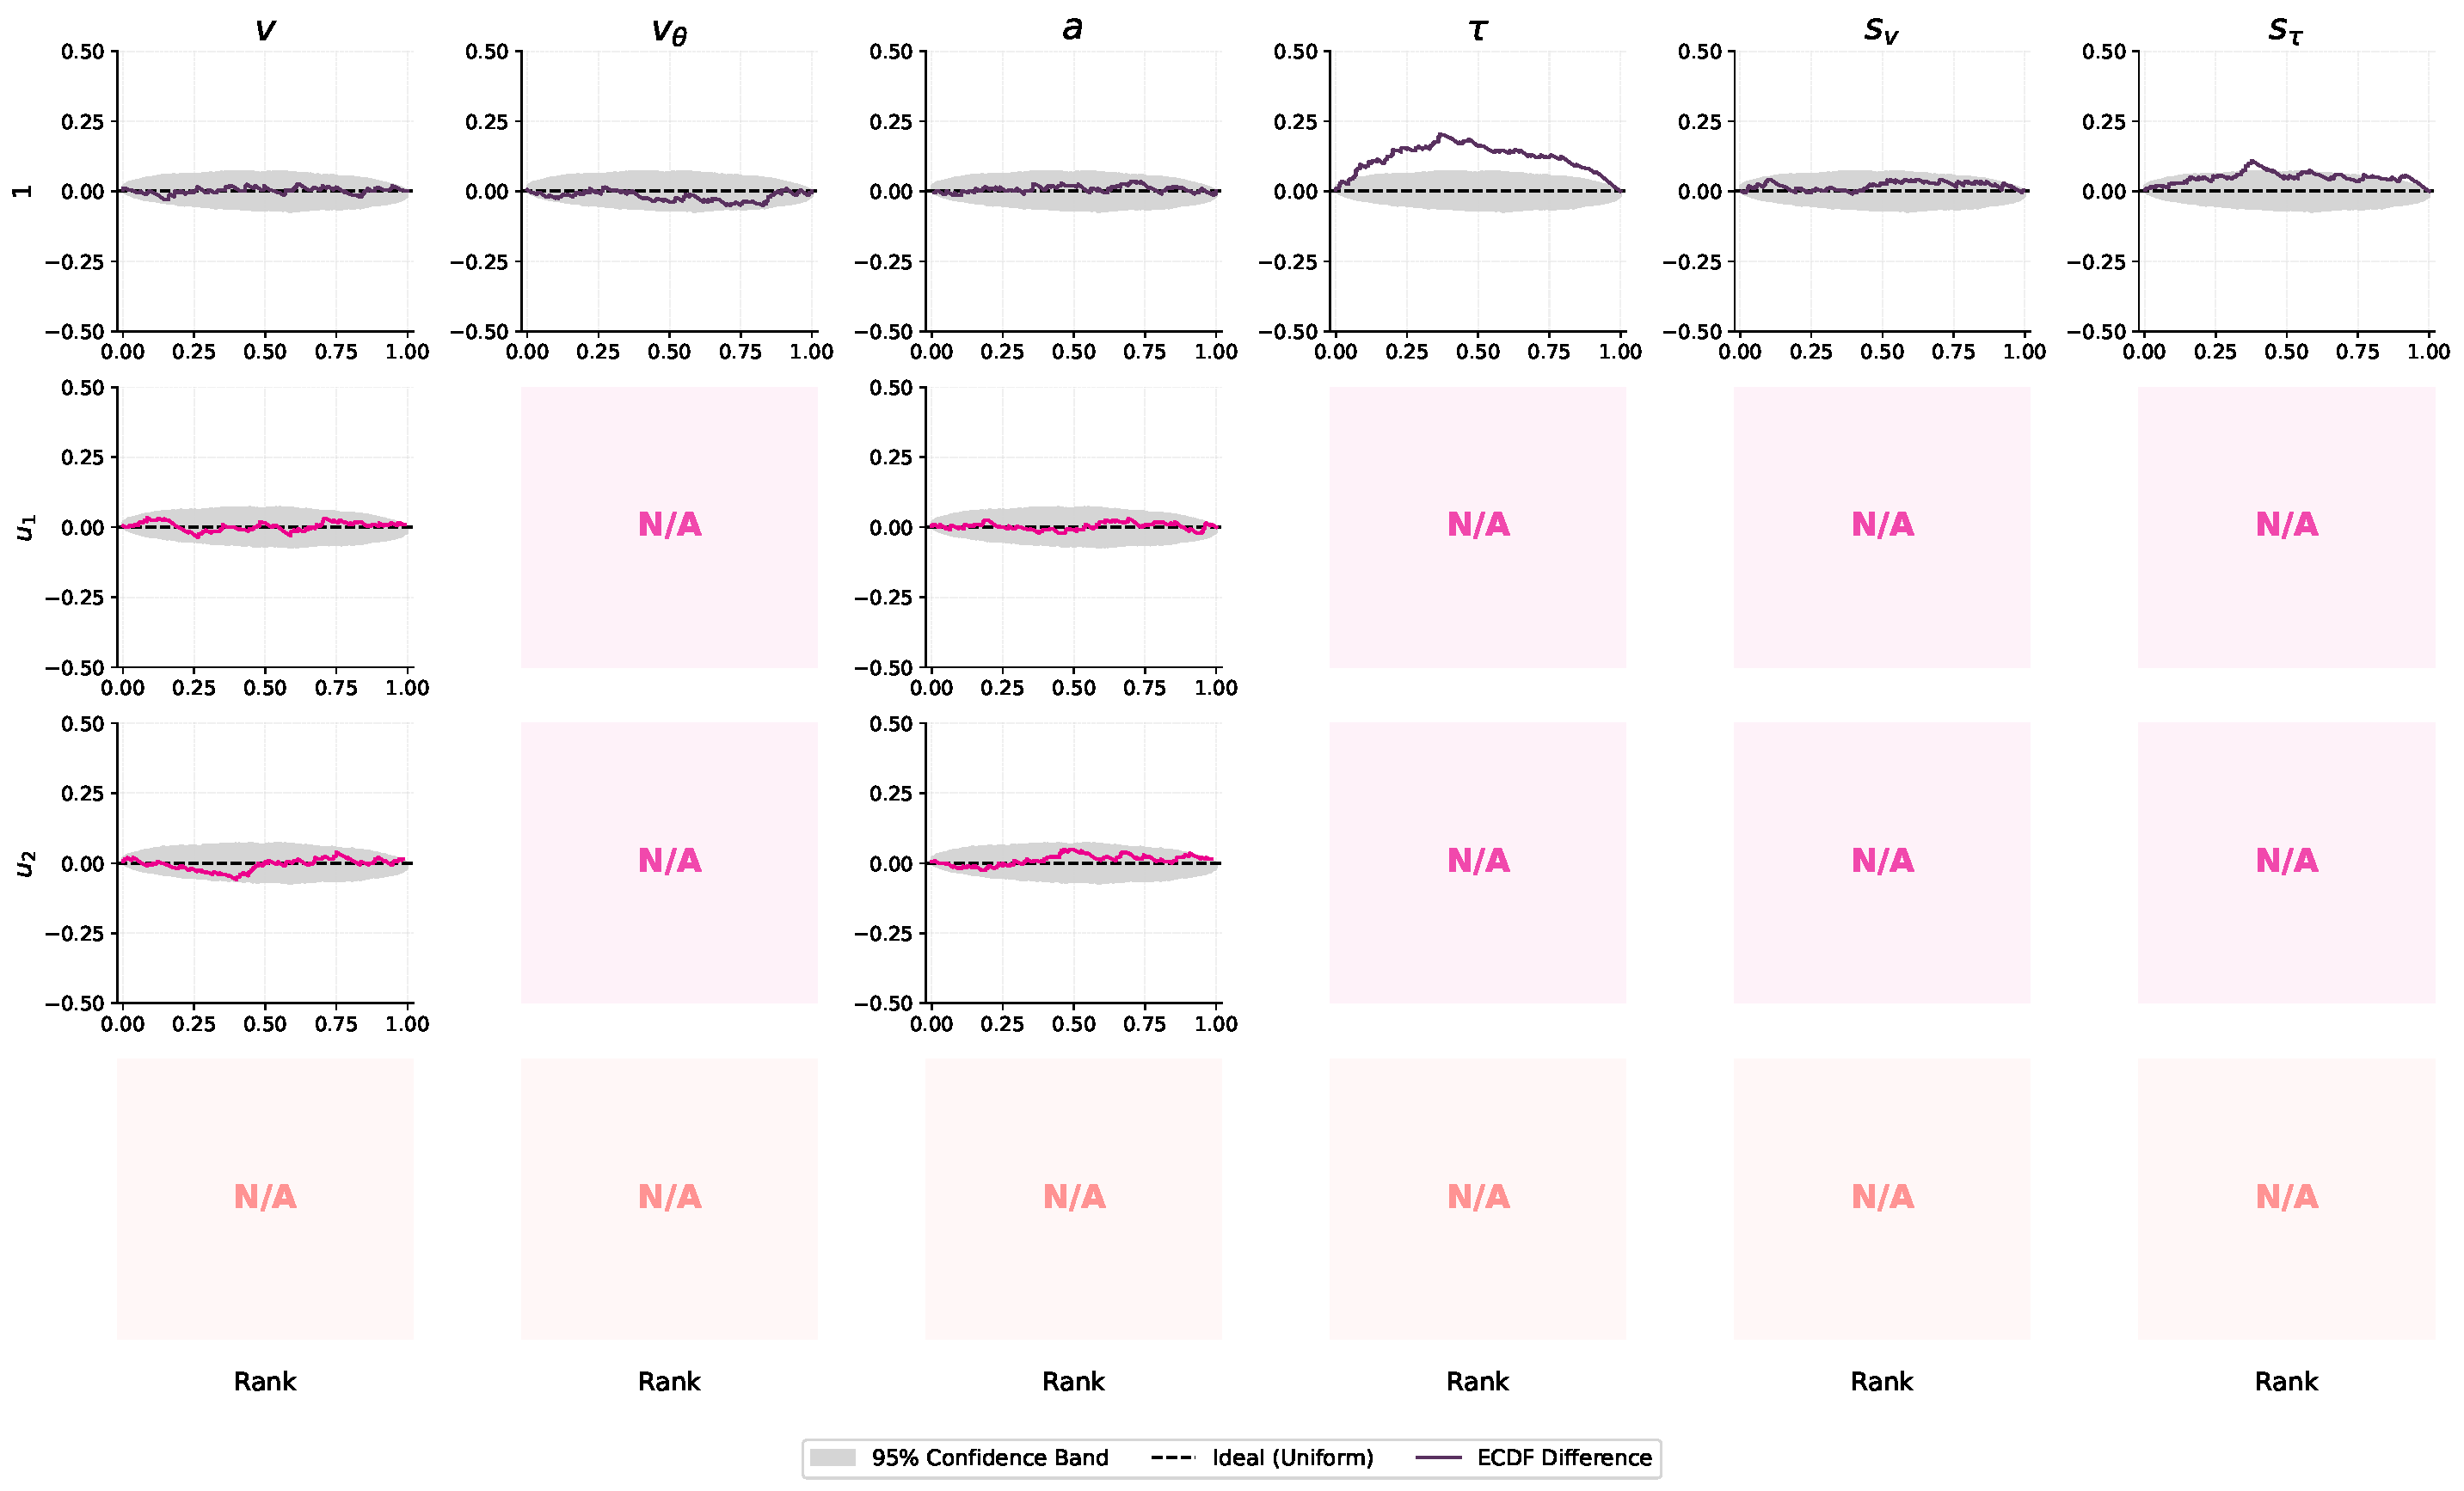
\includegraphics[width=0.99\linewidth]{figures/bf/cdm/regressed/cdm_family_regressed_bf_ecdf.pdf}
    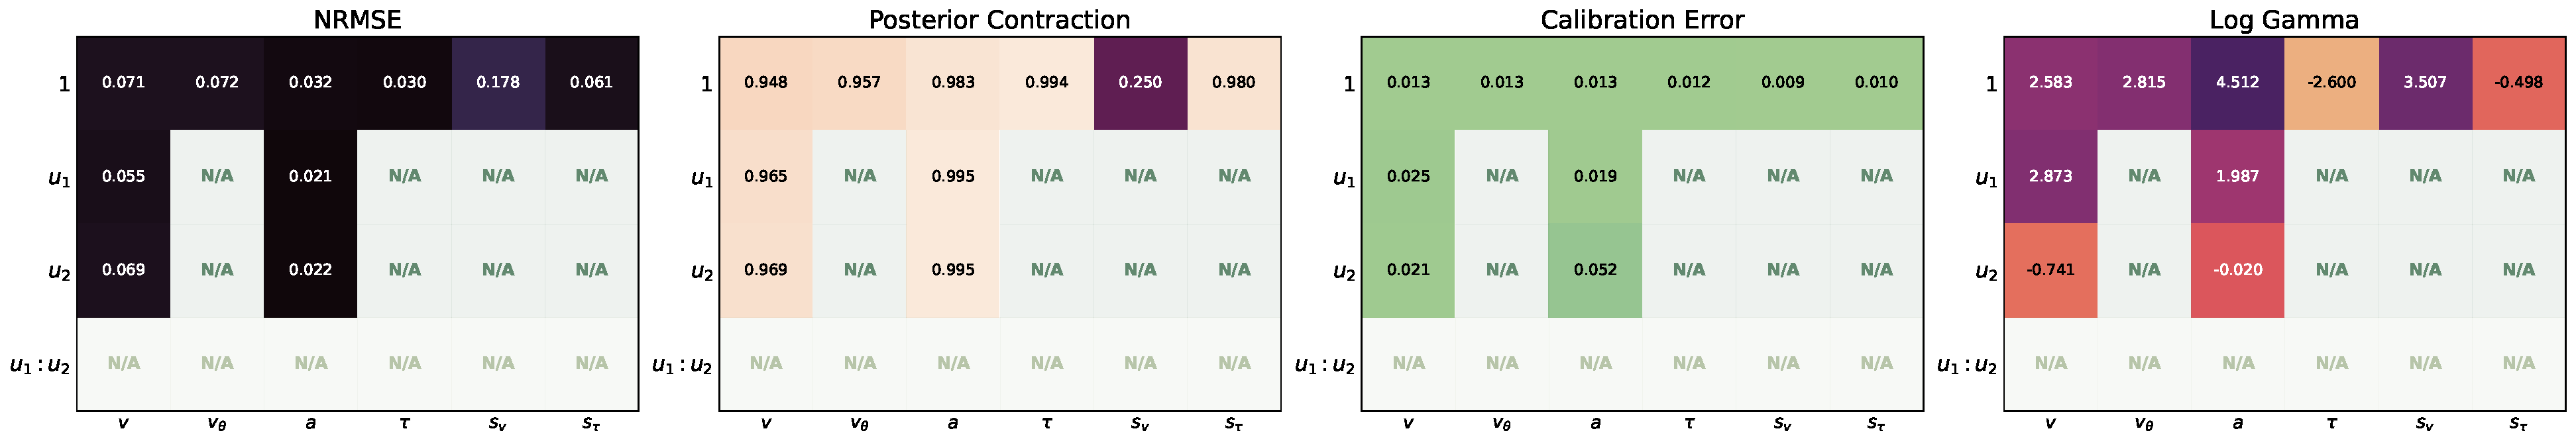
\includegraphics[width=0.99\linewidth]{figures/bf/cdm/regressed/cdm_family_regressed_bf_metrics.pdf}
    \caption{Parameter recovery (\emph{top}), calibration ECDF (\emph{middle}), and parameter-wise metrics (NRMSE, calibration error, and posterior contraction) for CDM baseline (Case \textbf{regressed}).}
    \label{fig:cdm-bf-regressed}
\end{figure}

\begin{figure}
    \centering
    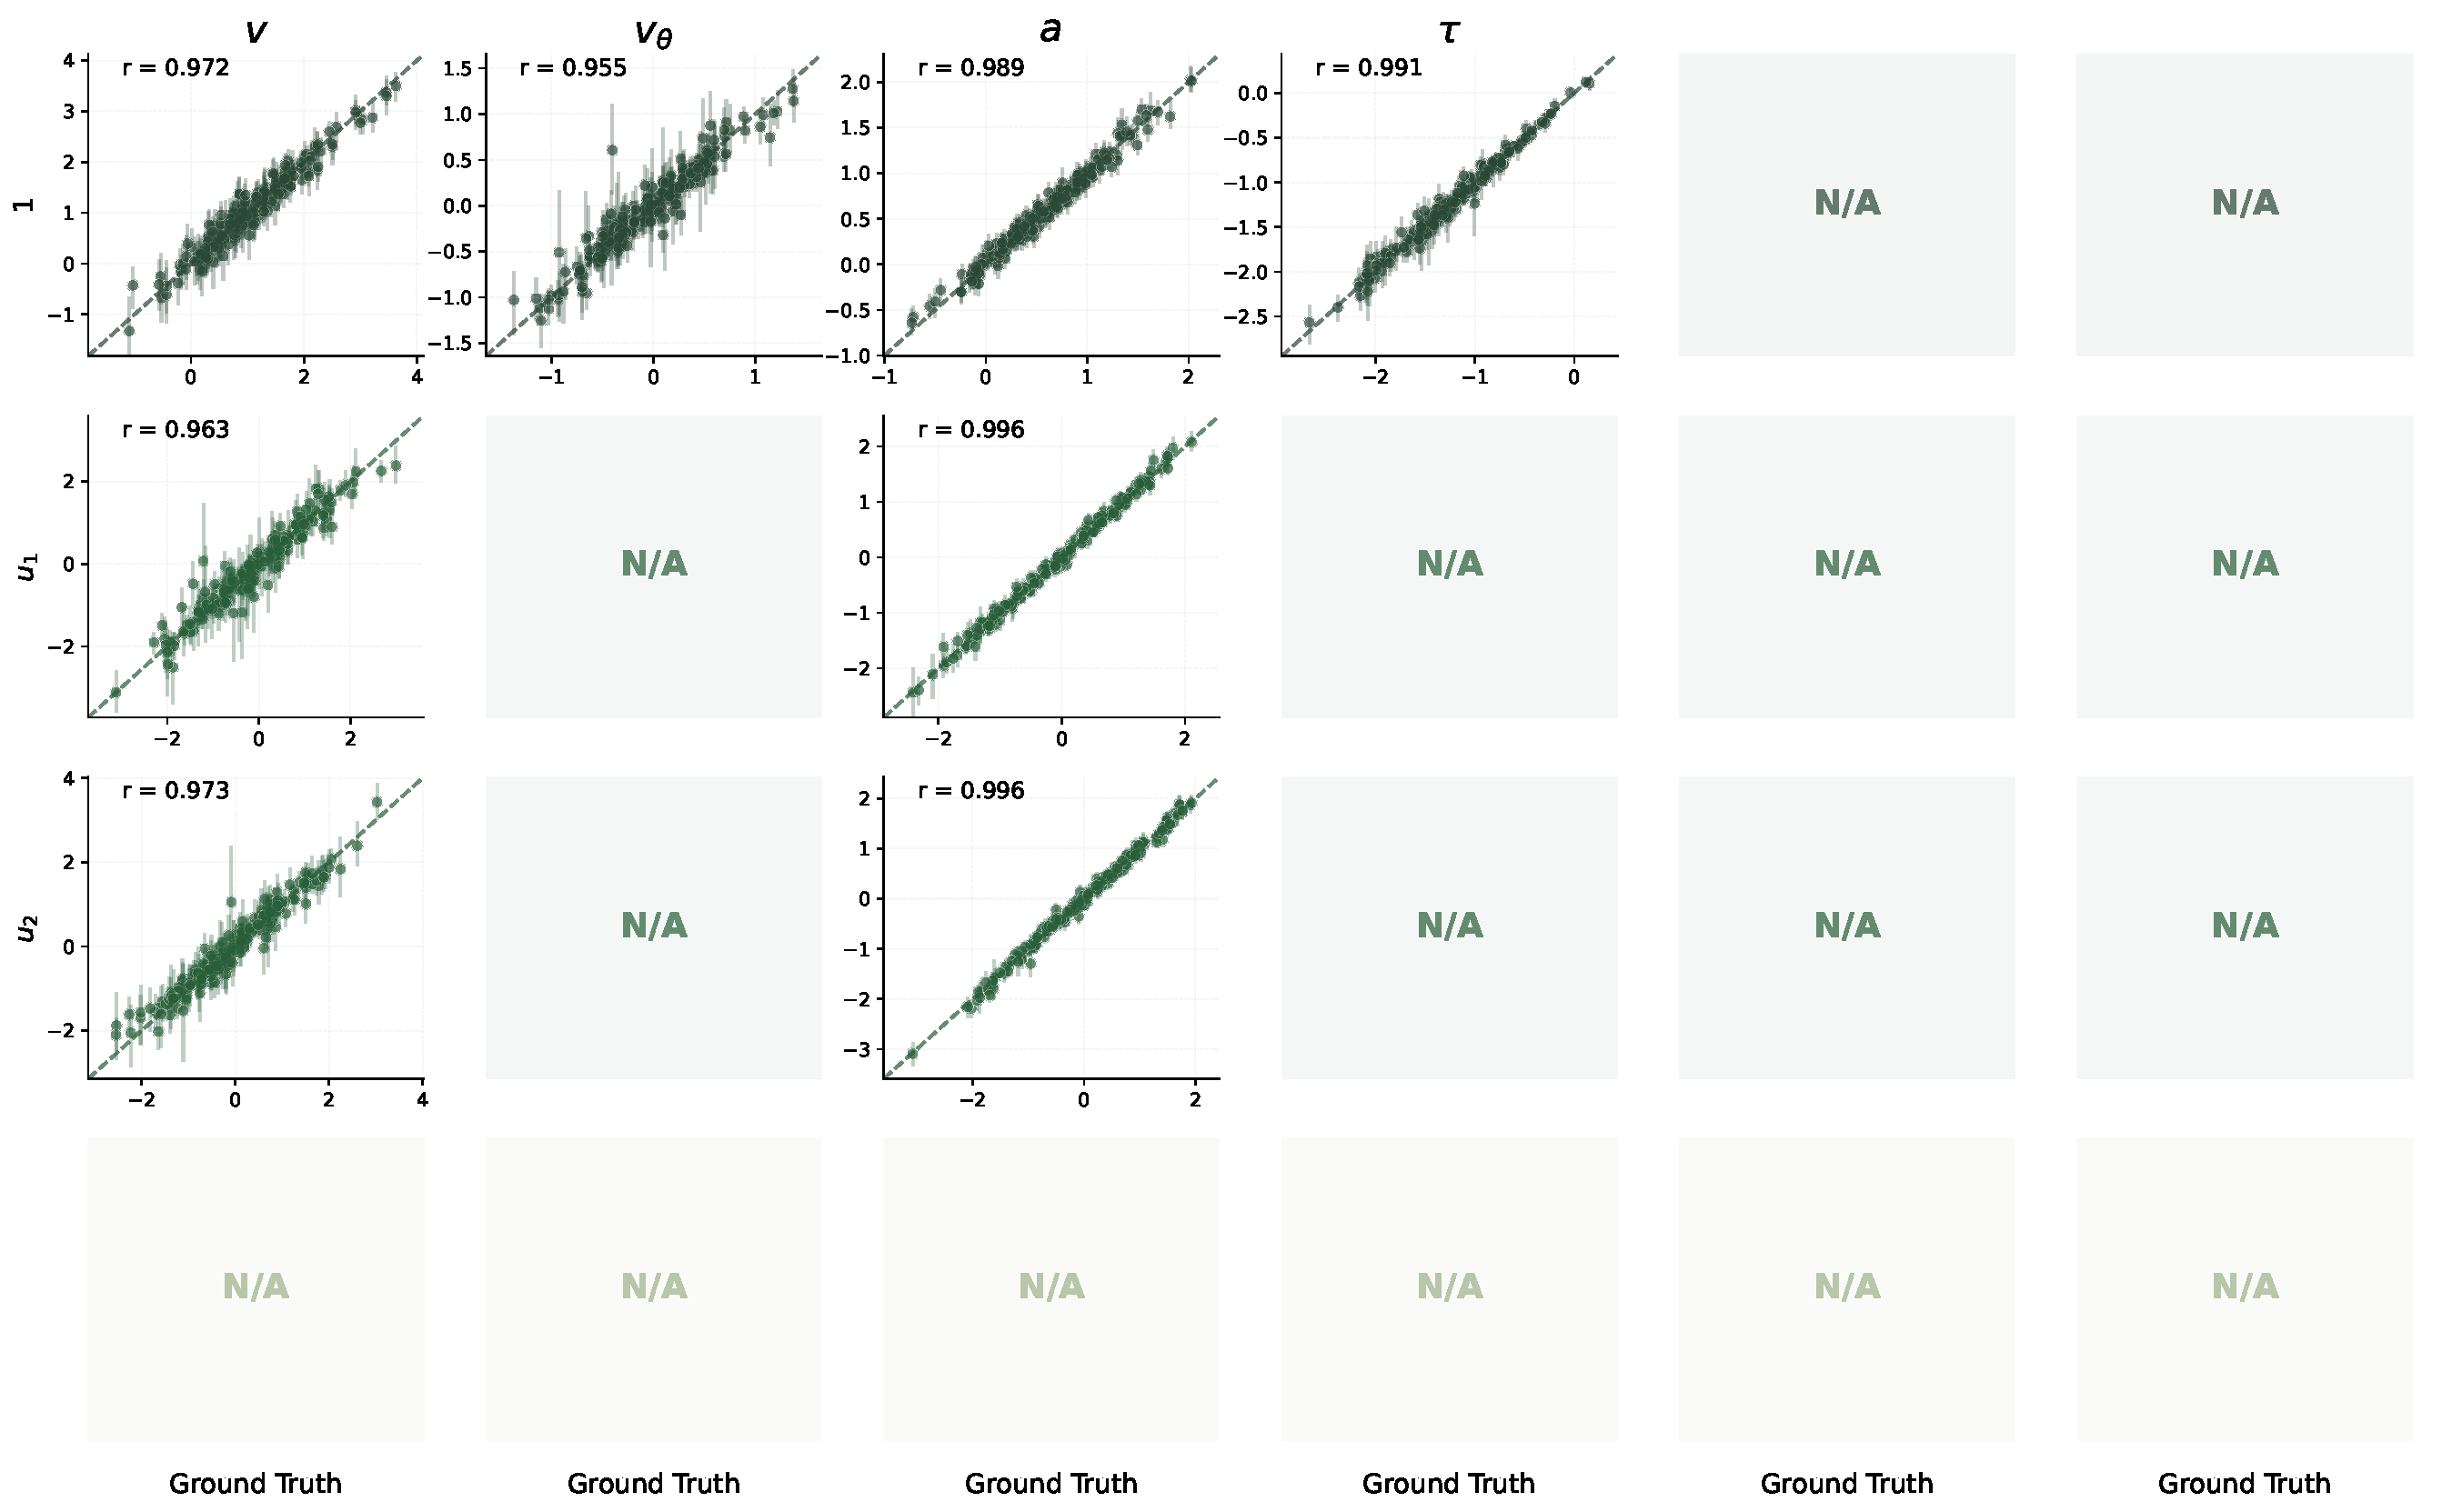
\includegraphics[width=0.99\linewidth]{figures/bf/cdm/fixed_regressed/cdm_family_fixed_regressed_bf_recovery.pdf}
    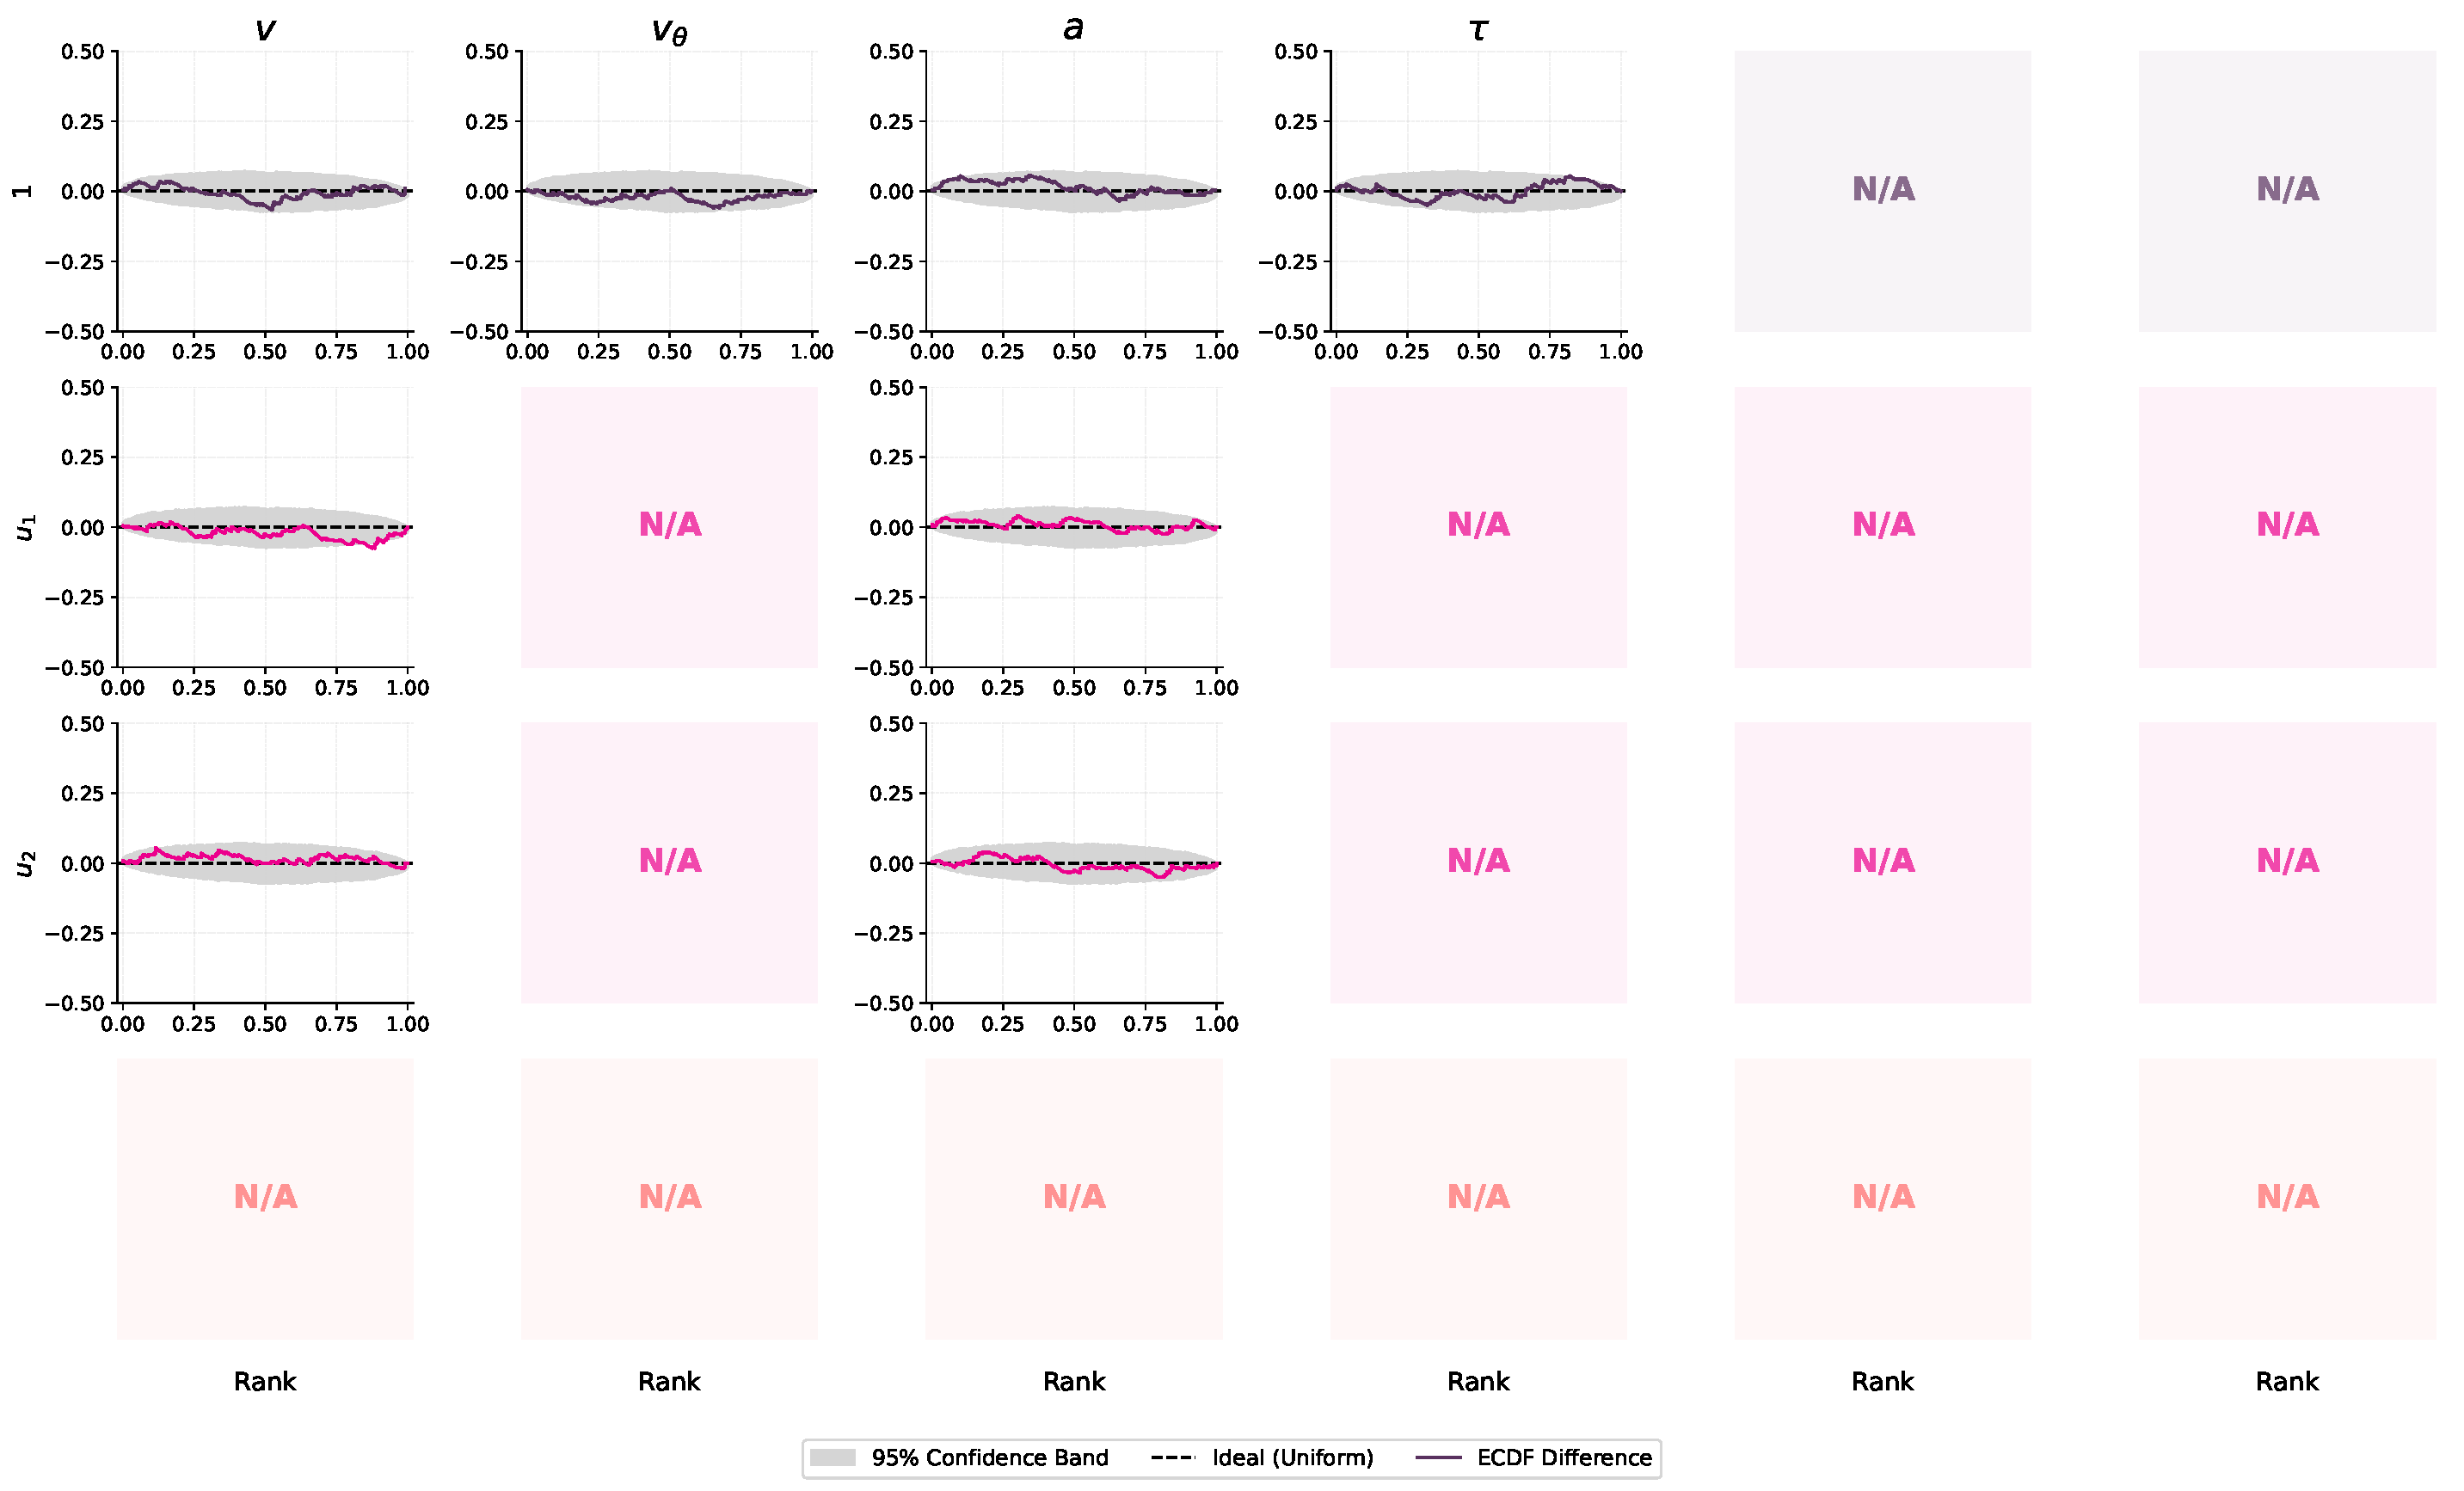
\includegraphics[width=0.99\linewidth]{figures/bf/cdm/fixed_regressed/cdm_family_fixed_regressed_bf_ecdf.pdf}
    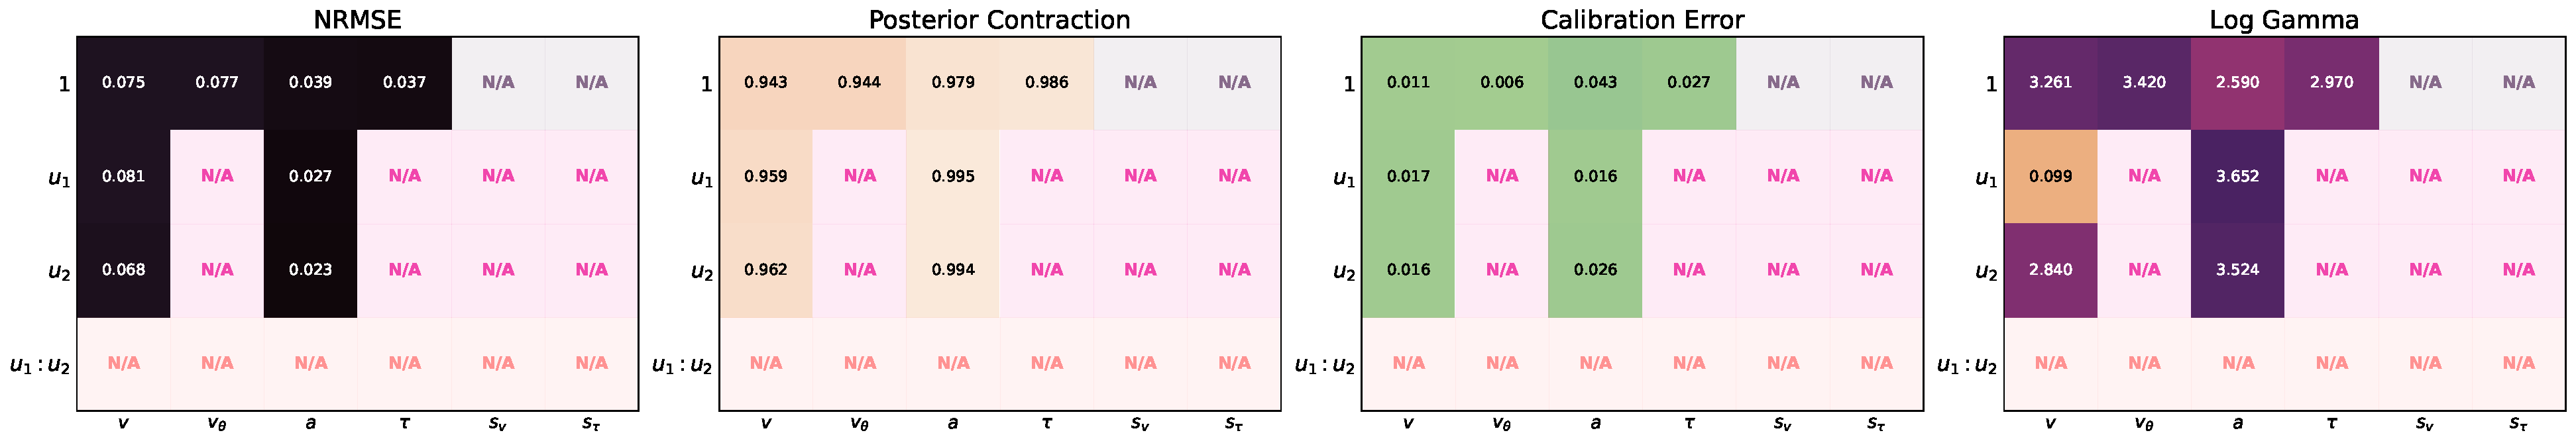
\includegraphics[width=0.99\linewidth]{figures/bf/cdm/fixed_regressed/cdm_family_fixed_regressed_bf_metrics.pdf}
    \caption{Parameter recovery (\emph{top}), calibration ECDF (\emph{middle}), and parameter-wise metrics (NRMSE, calibration error, and posterior contraction) for CDM baseline (Case \textbf{fixed\_regressed}).}
    \label{fig:cdm-bf-fixed-regressed}
\end{figure}

\begin{figure}
    \centering
    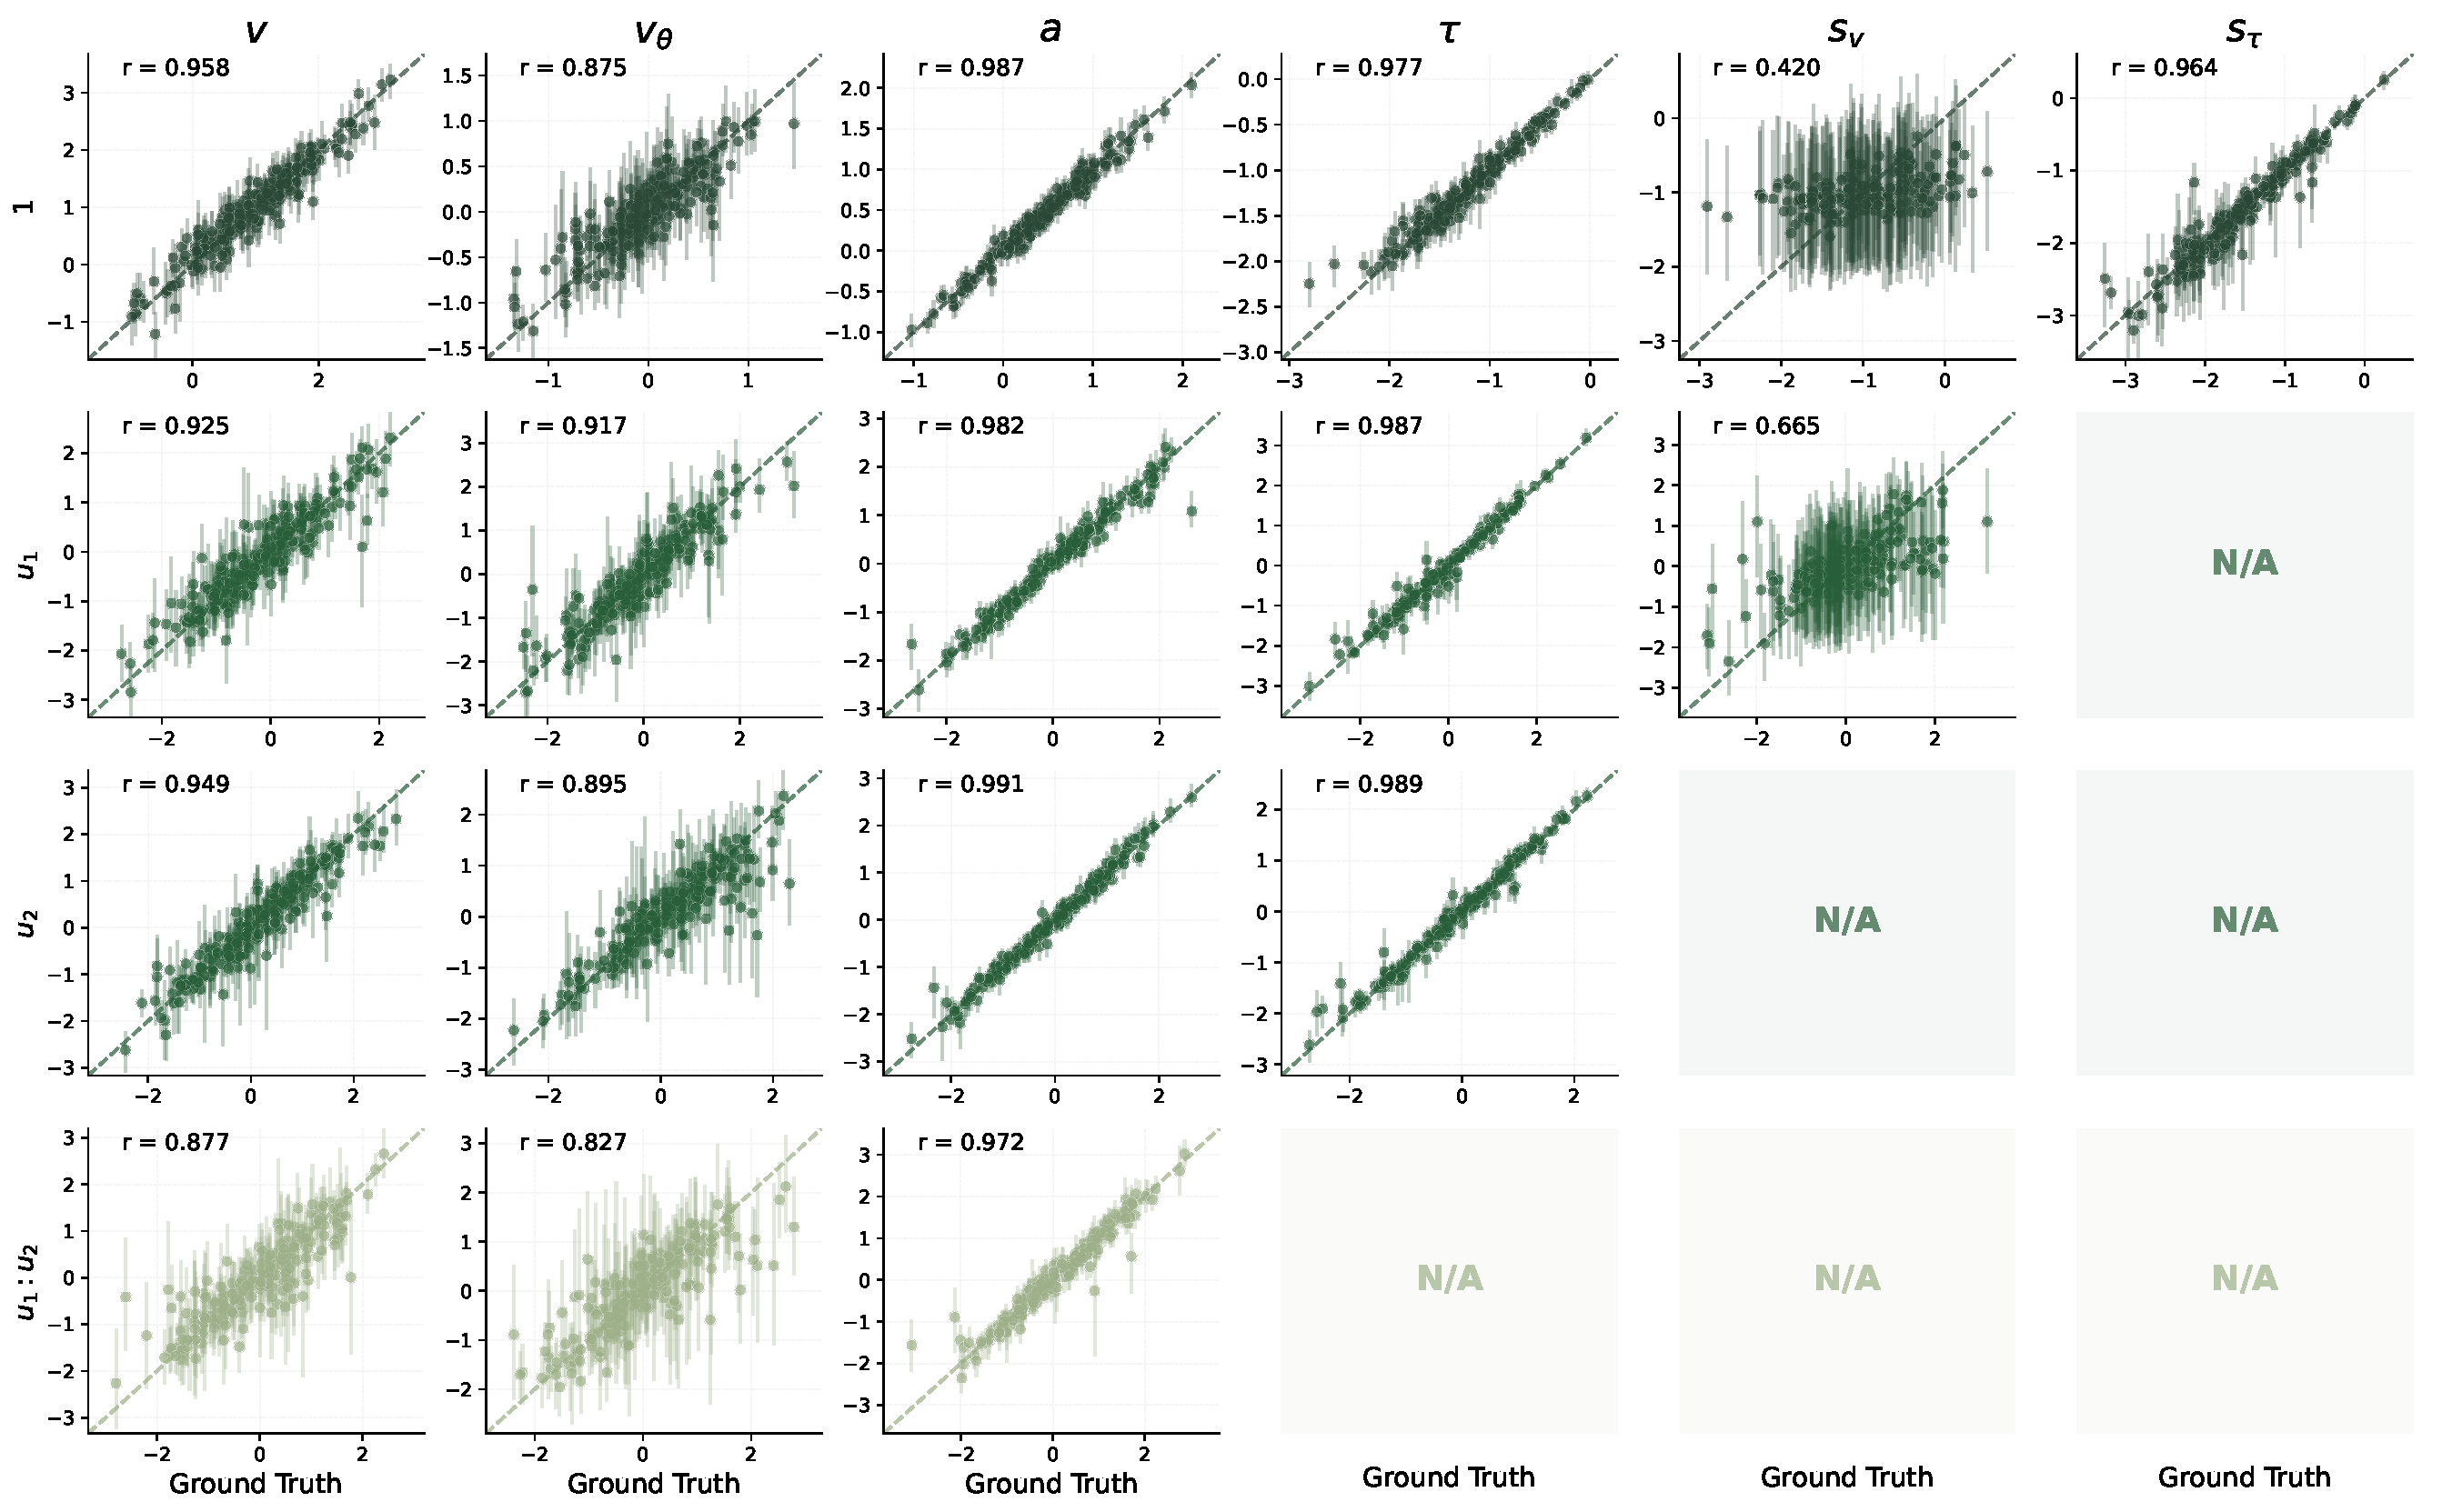
\includegraphics[width=0.99\linewidth]{figures/bf/cdm/interaction/cdm_family_interaction_bf_recovery.pdf}
    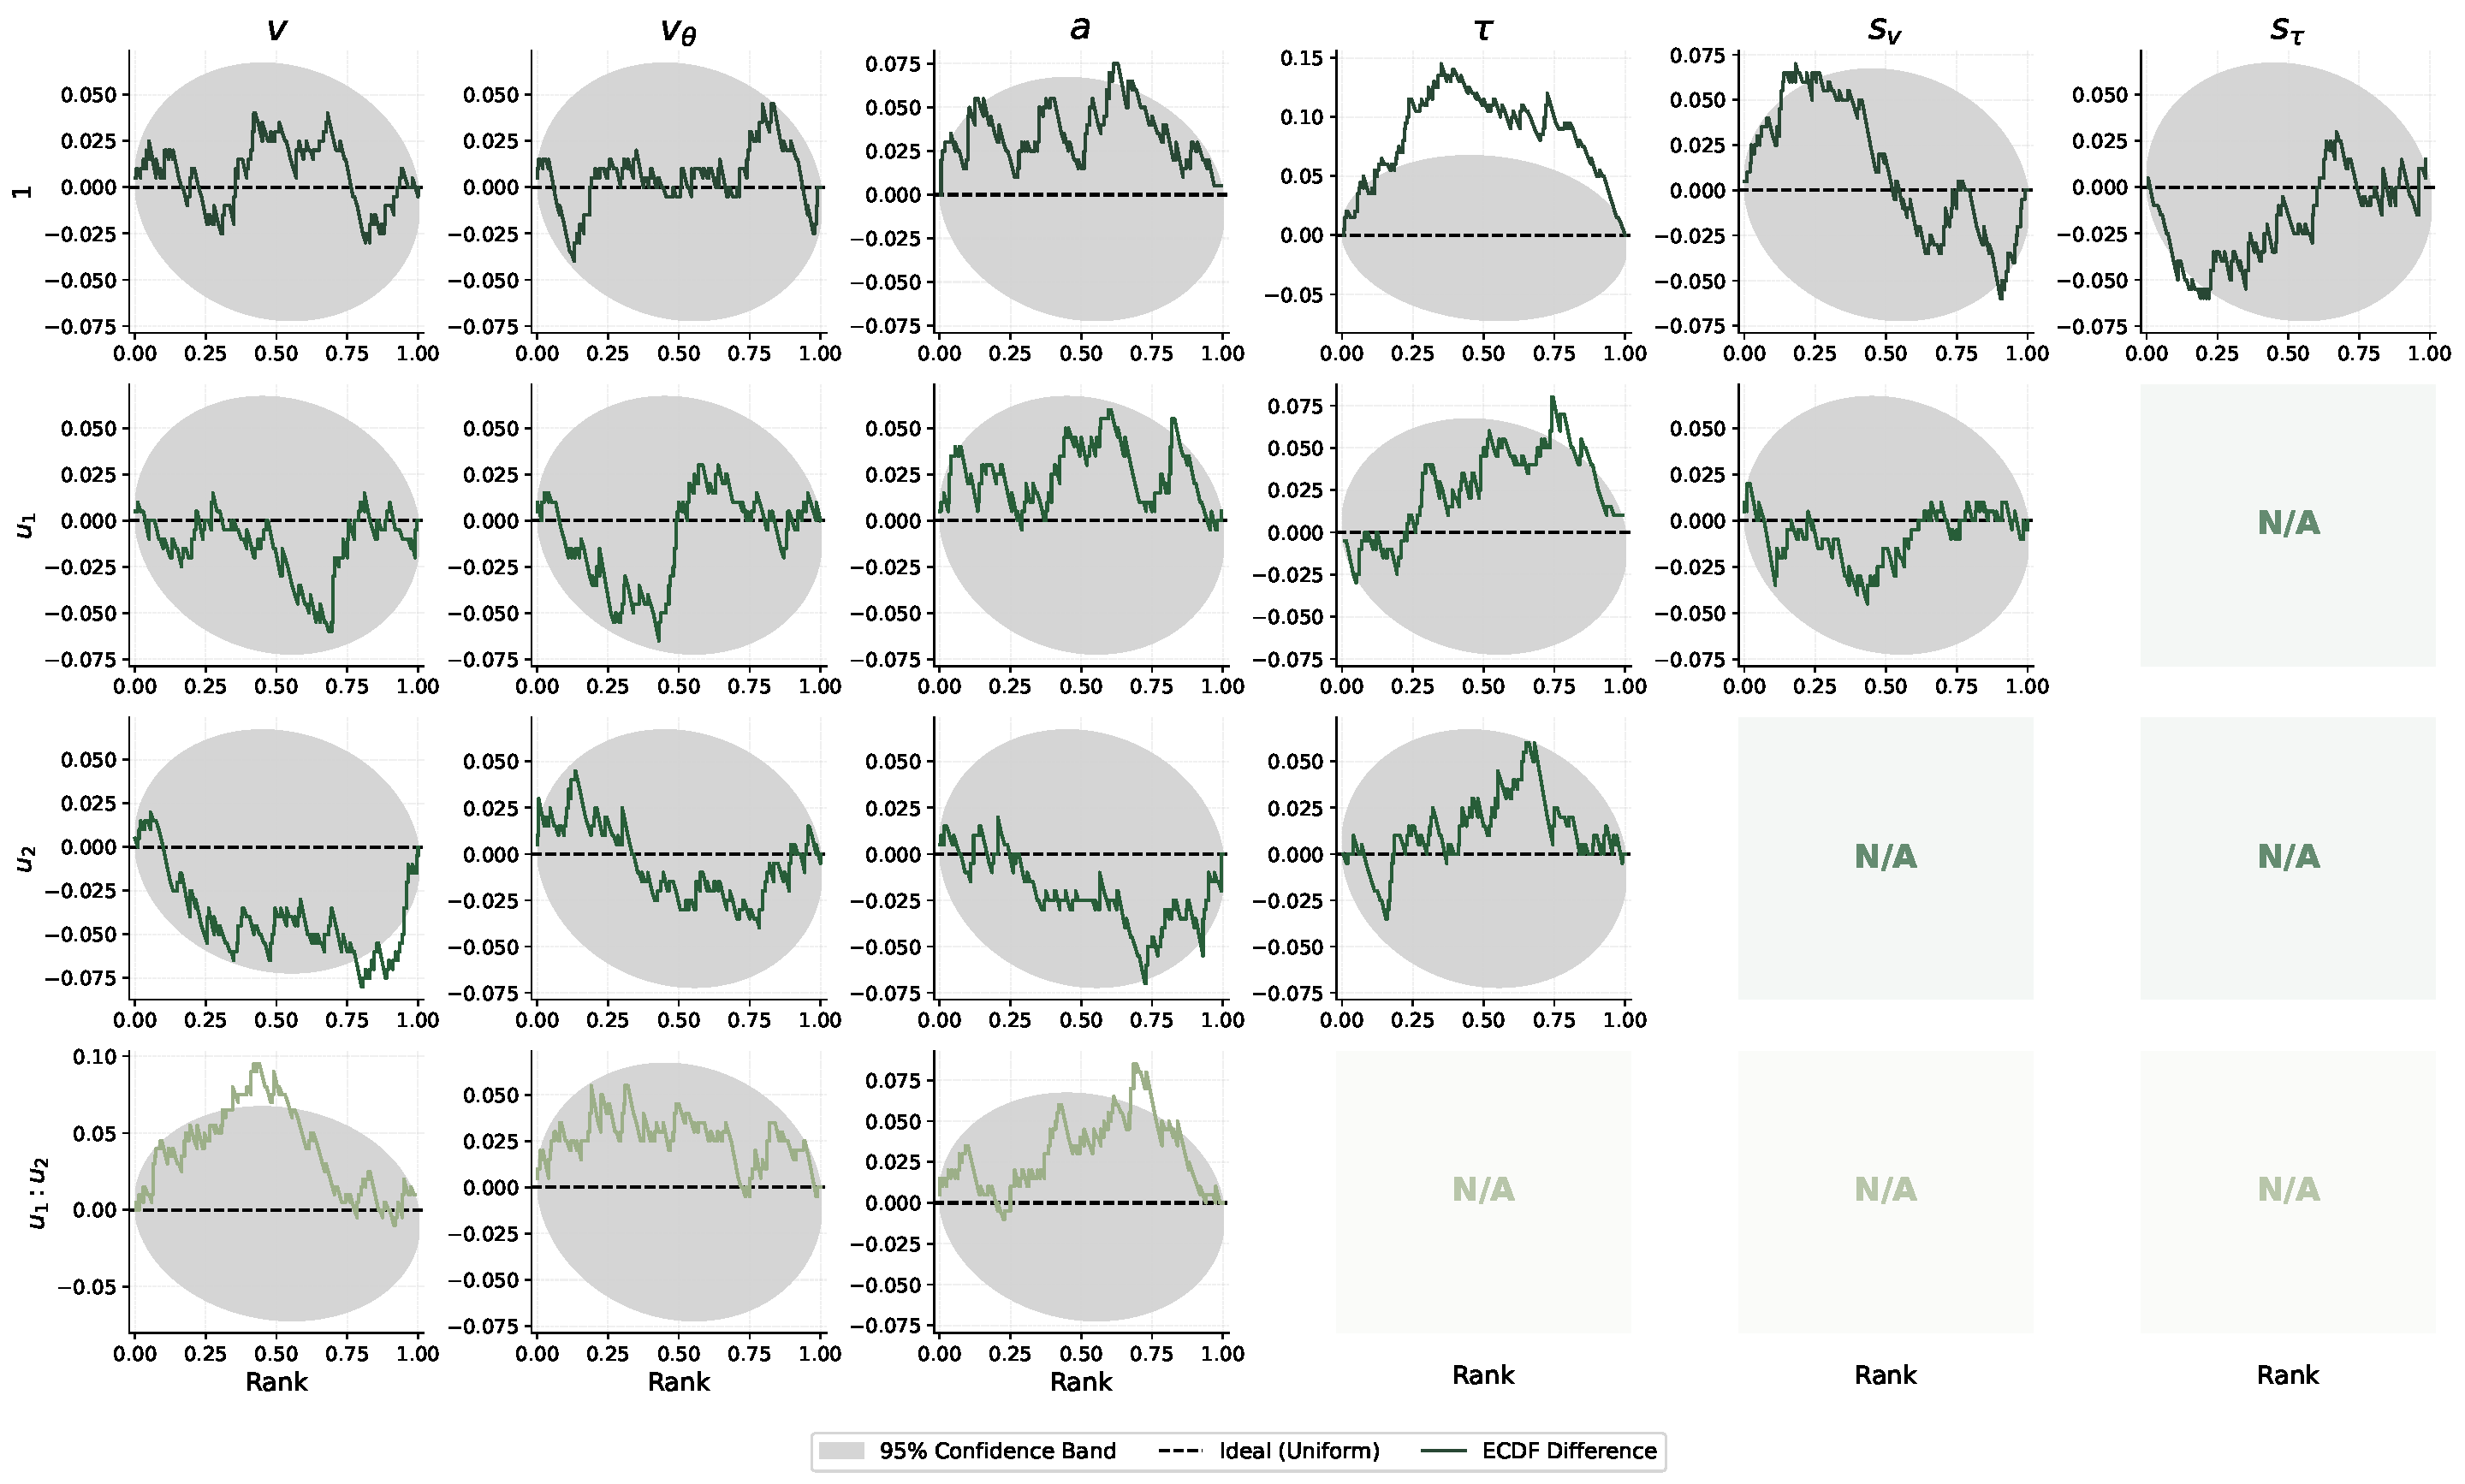
\includegraphics[width=0.99\linewidth]{figures/bf/cdm/interaction/cdm_family_interaction_bf_ecdf.pdf}
    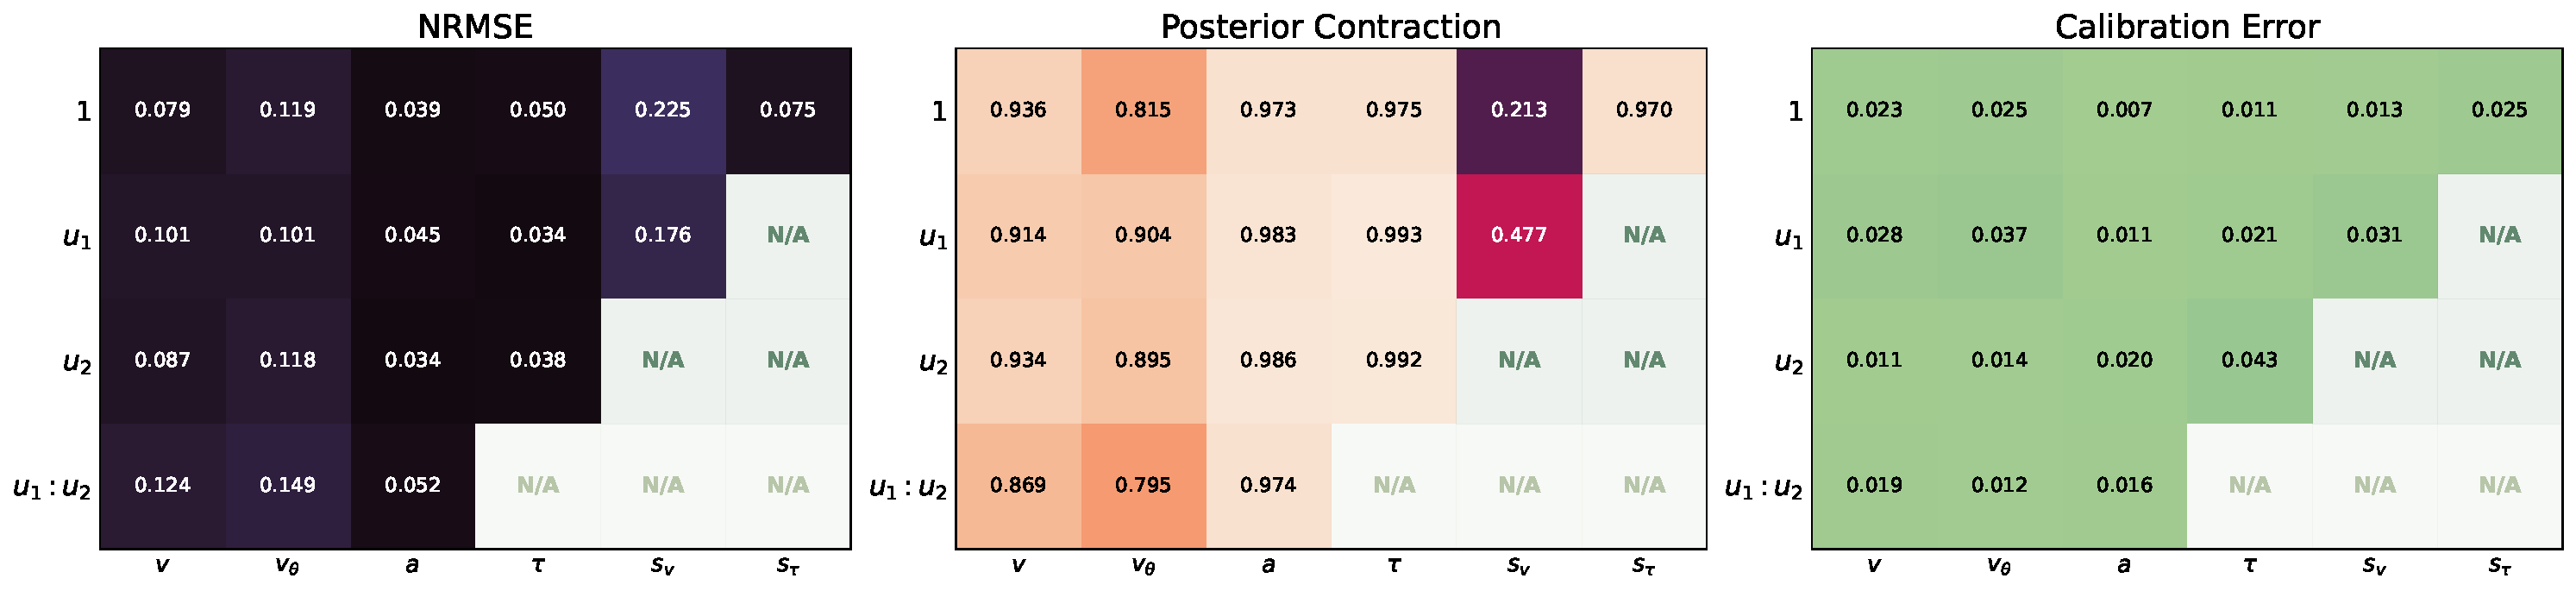
\includegraphics[width=0.99\linewidth]{figures/bf/cdm/interaction/cdm_family_interaction_bf_metrics.pdf}
    \caption{Parameter recovery (\emph{top}), calibration ECDF (\emph{middle}), and parameter-wise metrics (NRMSE, calibration error, and posterior contraction) for CDM baseline (Case \textbf{interaction}).}
    \label{fig:cdm-bf-interaction}
\end{figure}

% ========================================
% CDM MODEL FAMILY (fm)
% ========================================

\begin{figure}
    \centering
    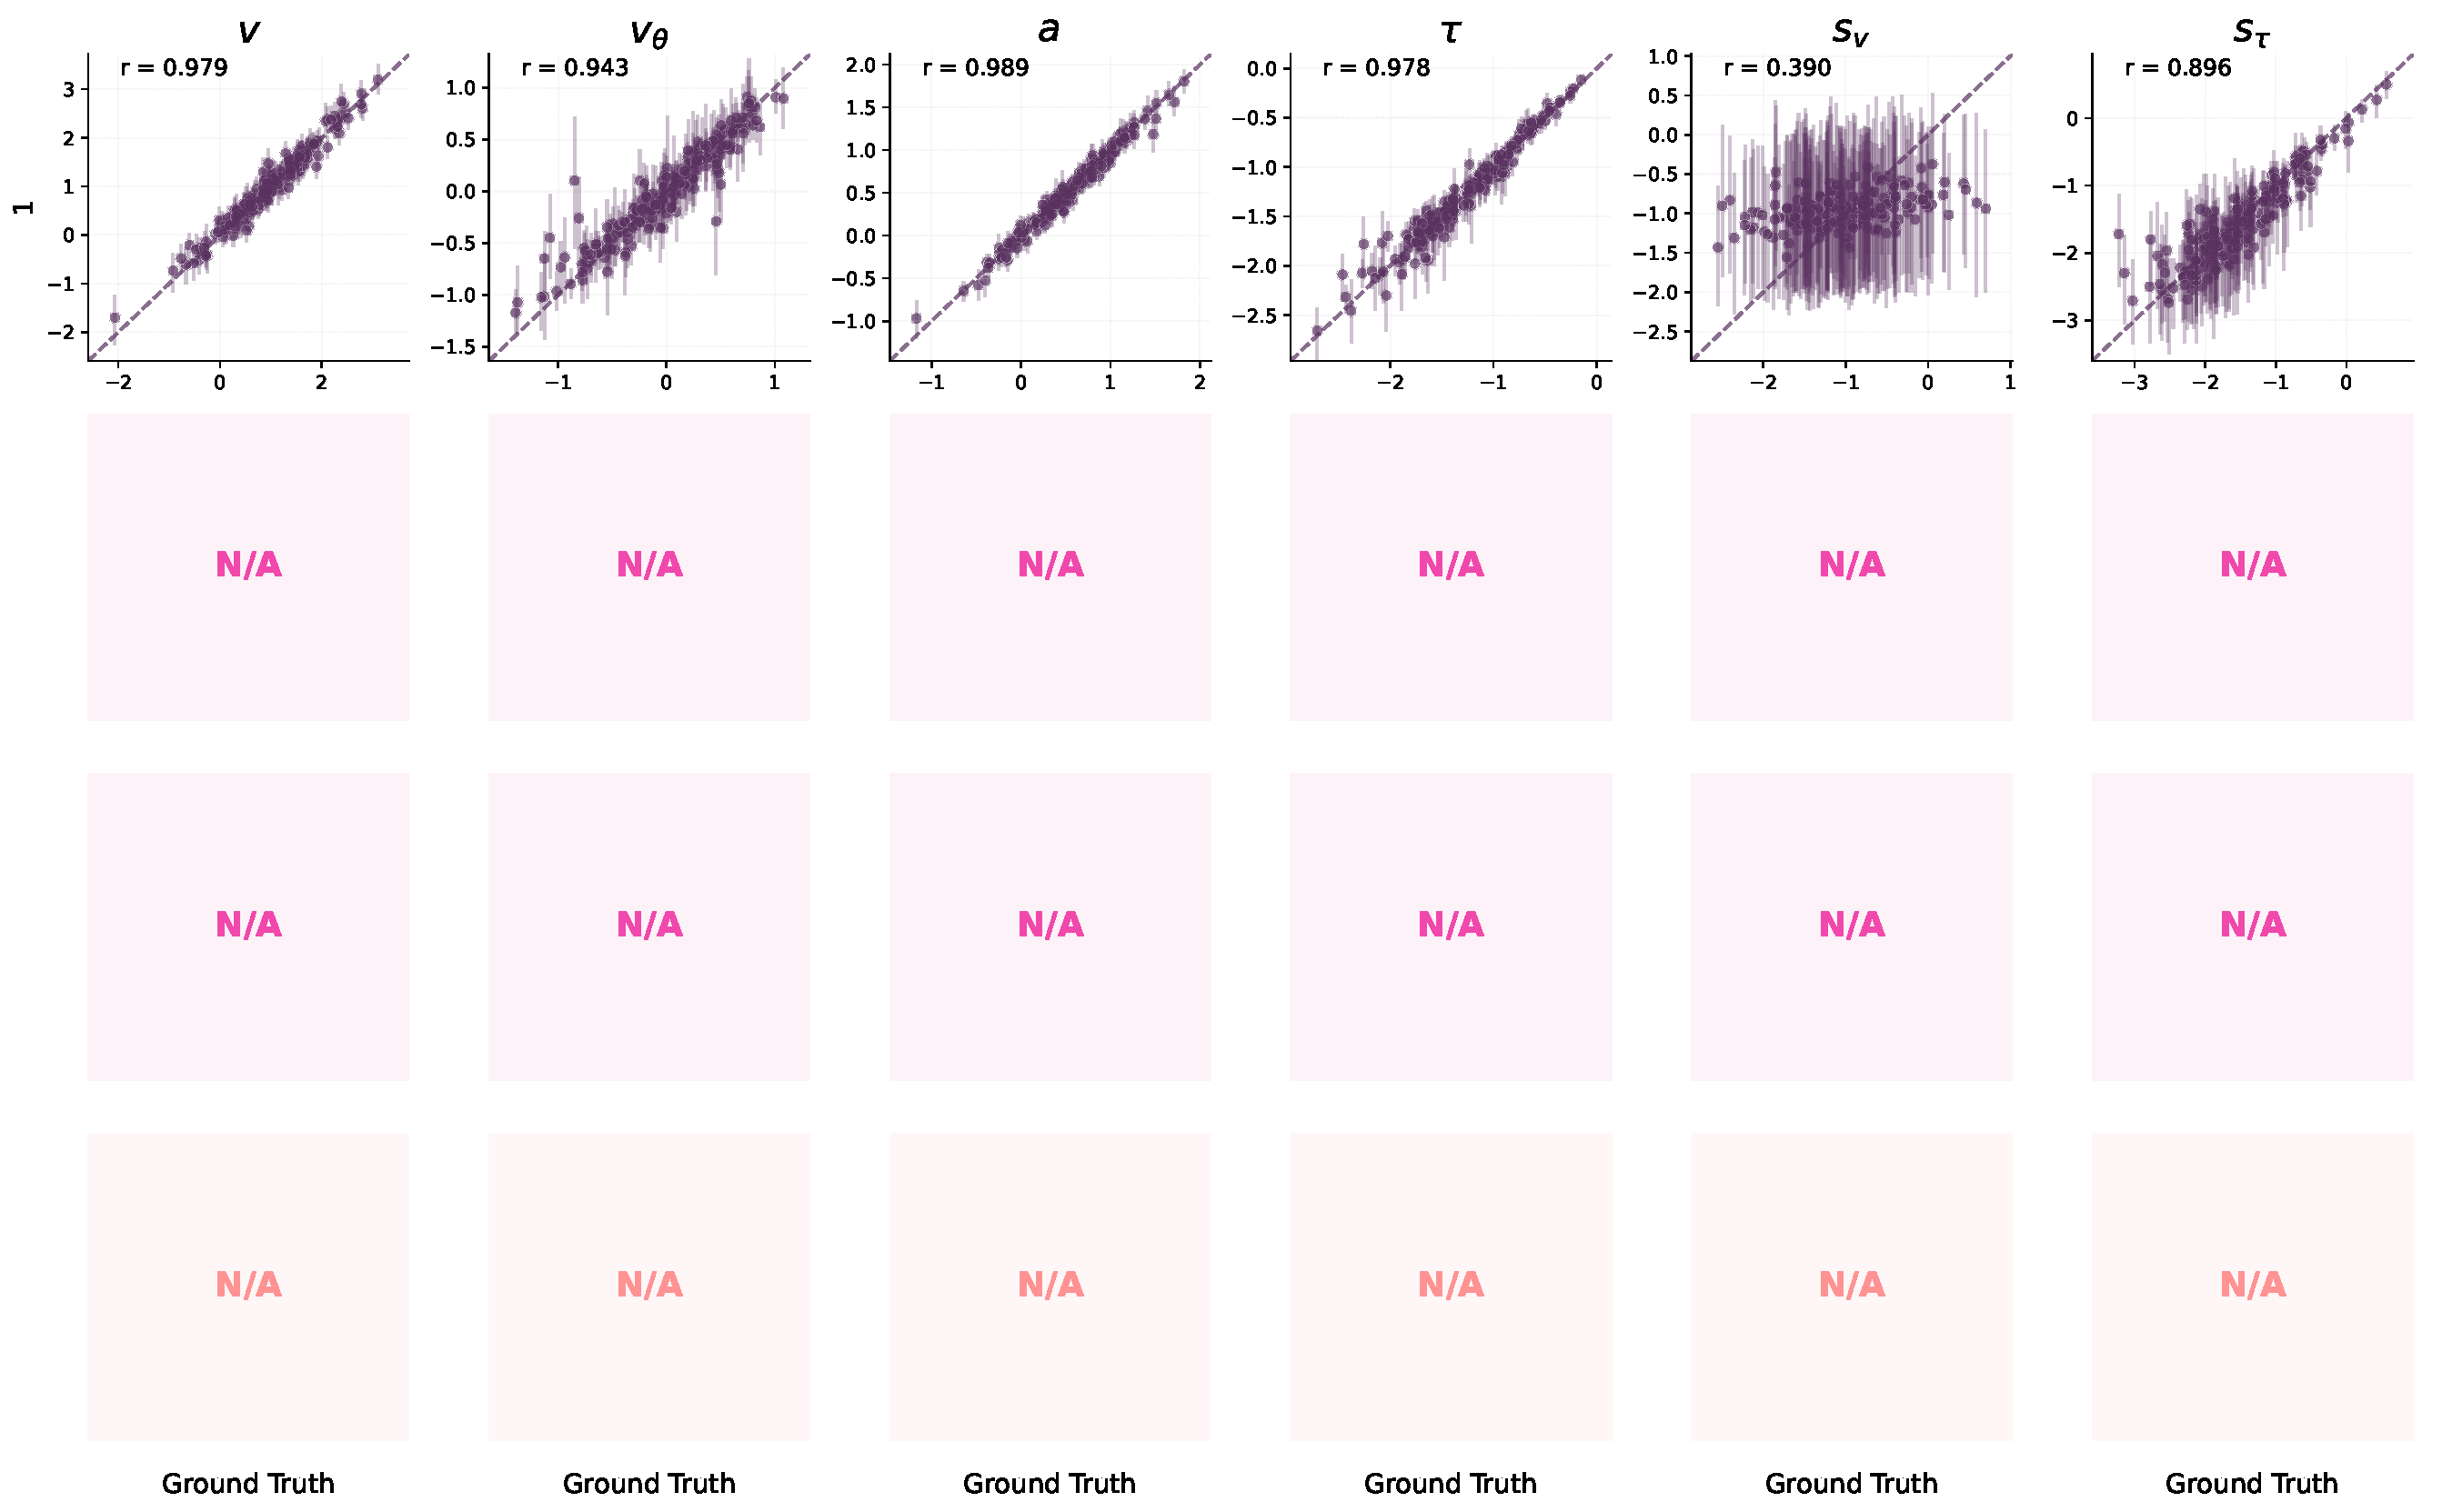
\includegraphics[width=0.99\linewidth]{figures/fm/cdm/intercept_only/cdm_family_intercept_only_fm_mixed_recovery.pdf}
    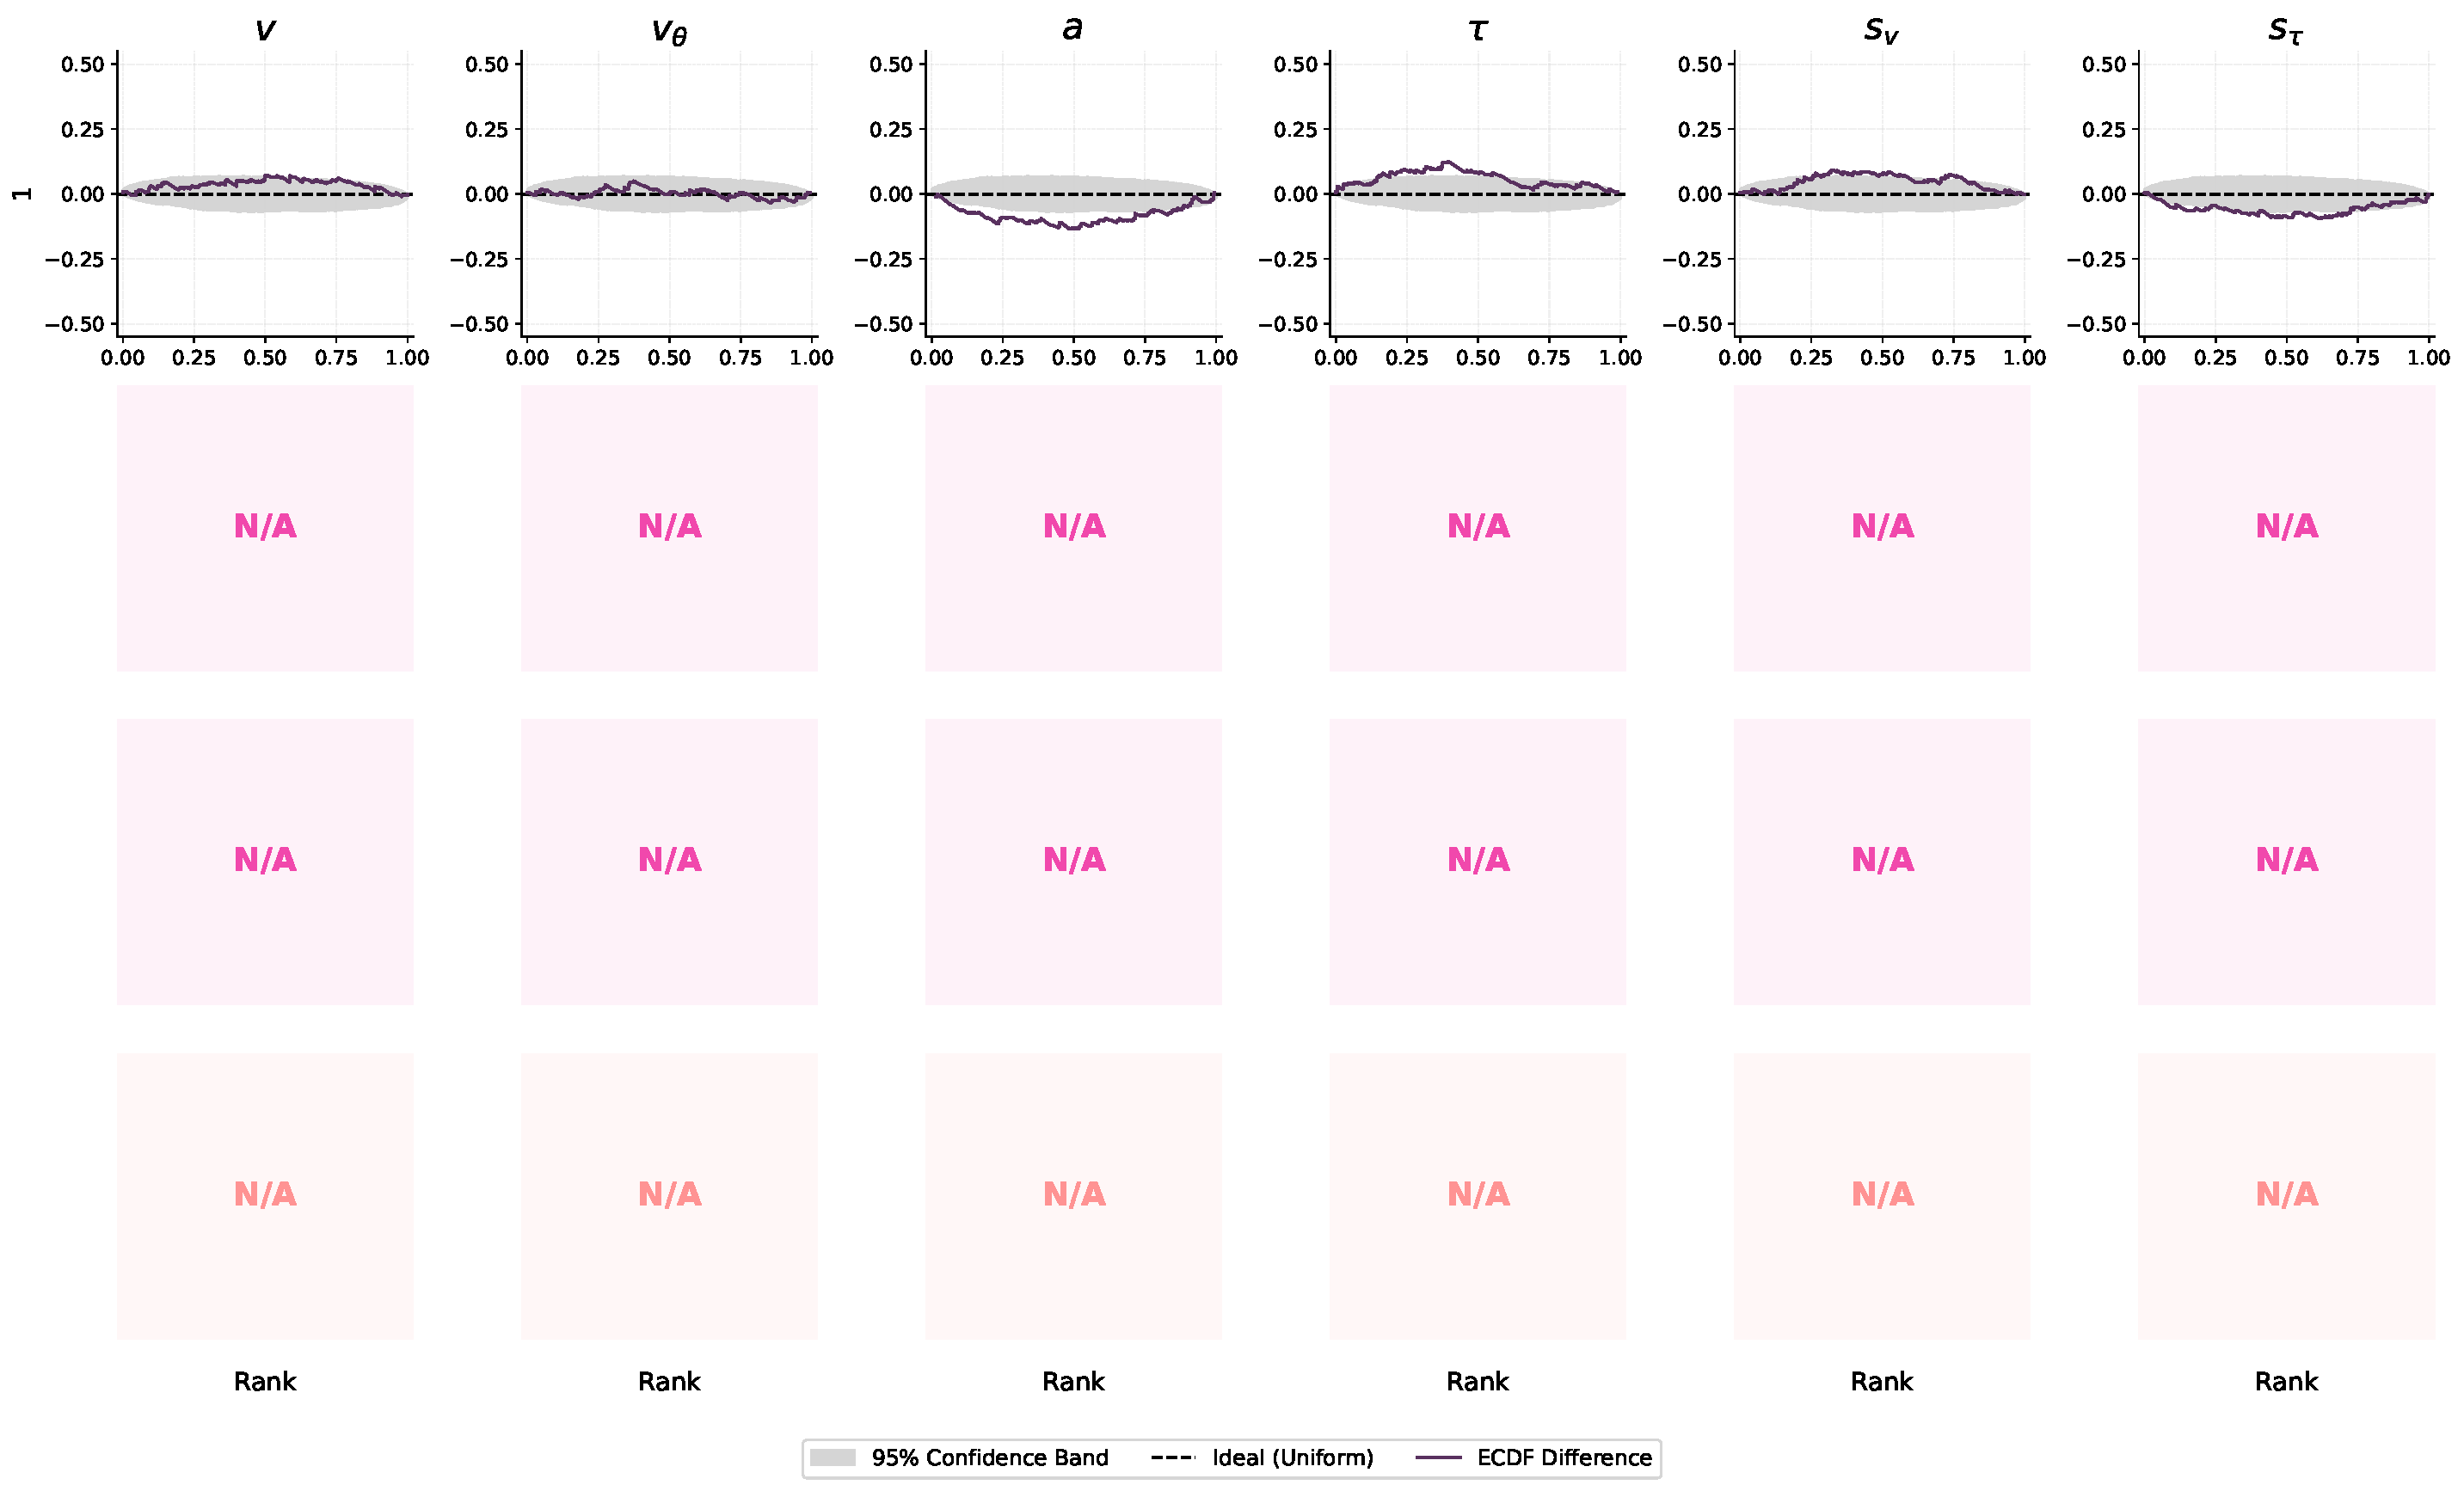
\includegraphics[width=0.99\linewidth]{figures/fm/cdm/intercept_only/cdm_family_intercept_only_fm_mixed_ecdf.pdf}
    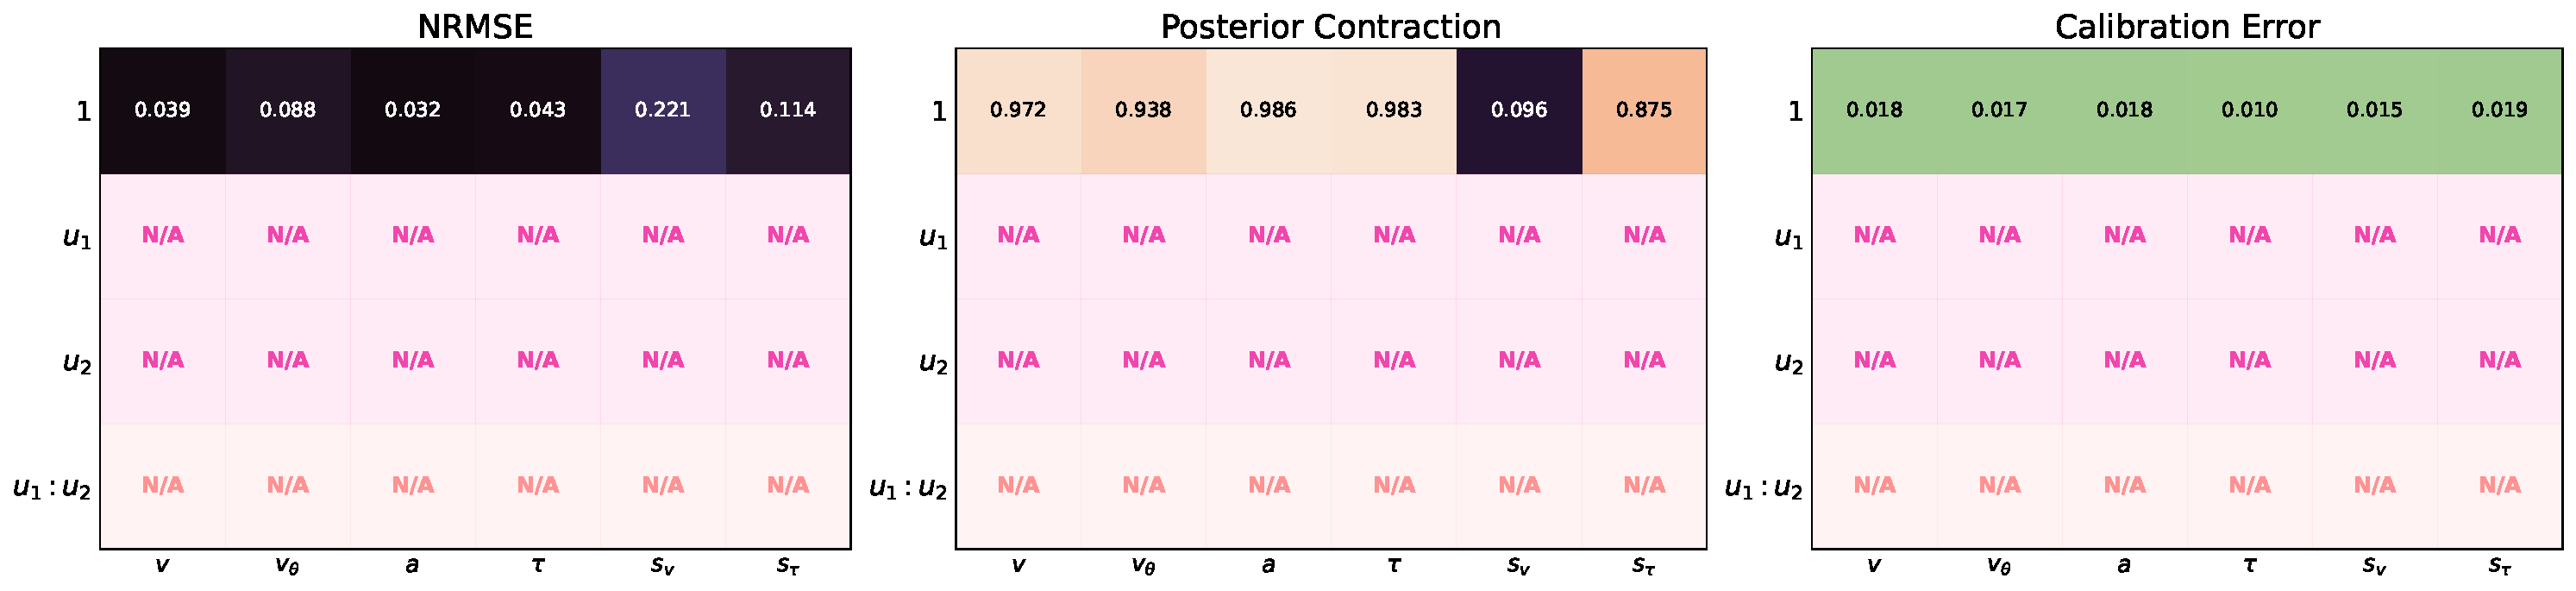
\includegraphics[width=0.99\linewidth]{figures/fm/cdm/intercept_only/cdm_family_intercept_only_fm_mixed_metrics.pdf}
    \caption{Parameter recovery (\emph{top}), calibration ECDF (\emph{middle}), and parameter-wise metrics (NRMSE, calibration error, and posterior contraction) for CDM model family (Case \textbf{intercept\_only}).}
    \label{fig:cdm-fm-intercept-only}
\end{figure}

\begin{figure}
    \centering
    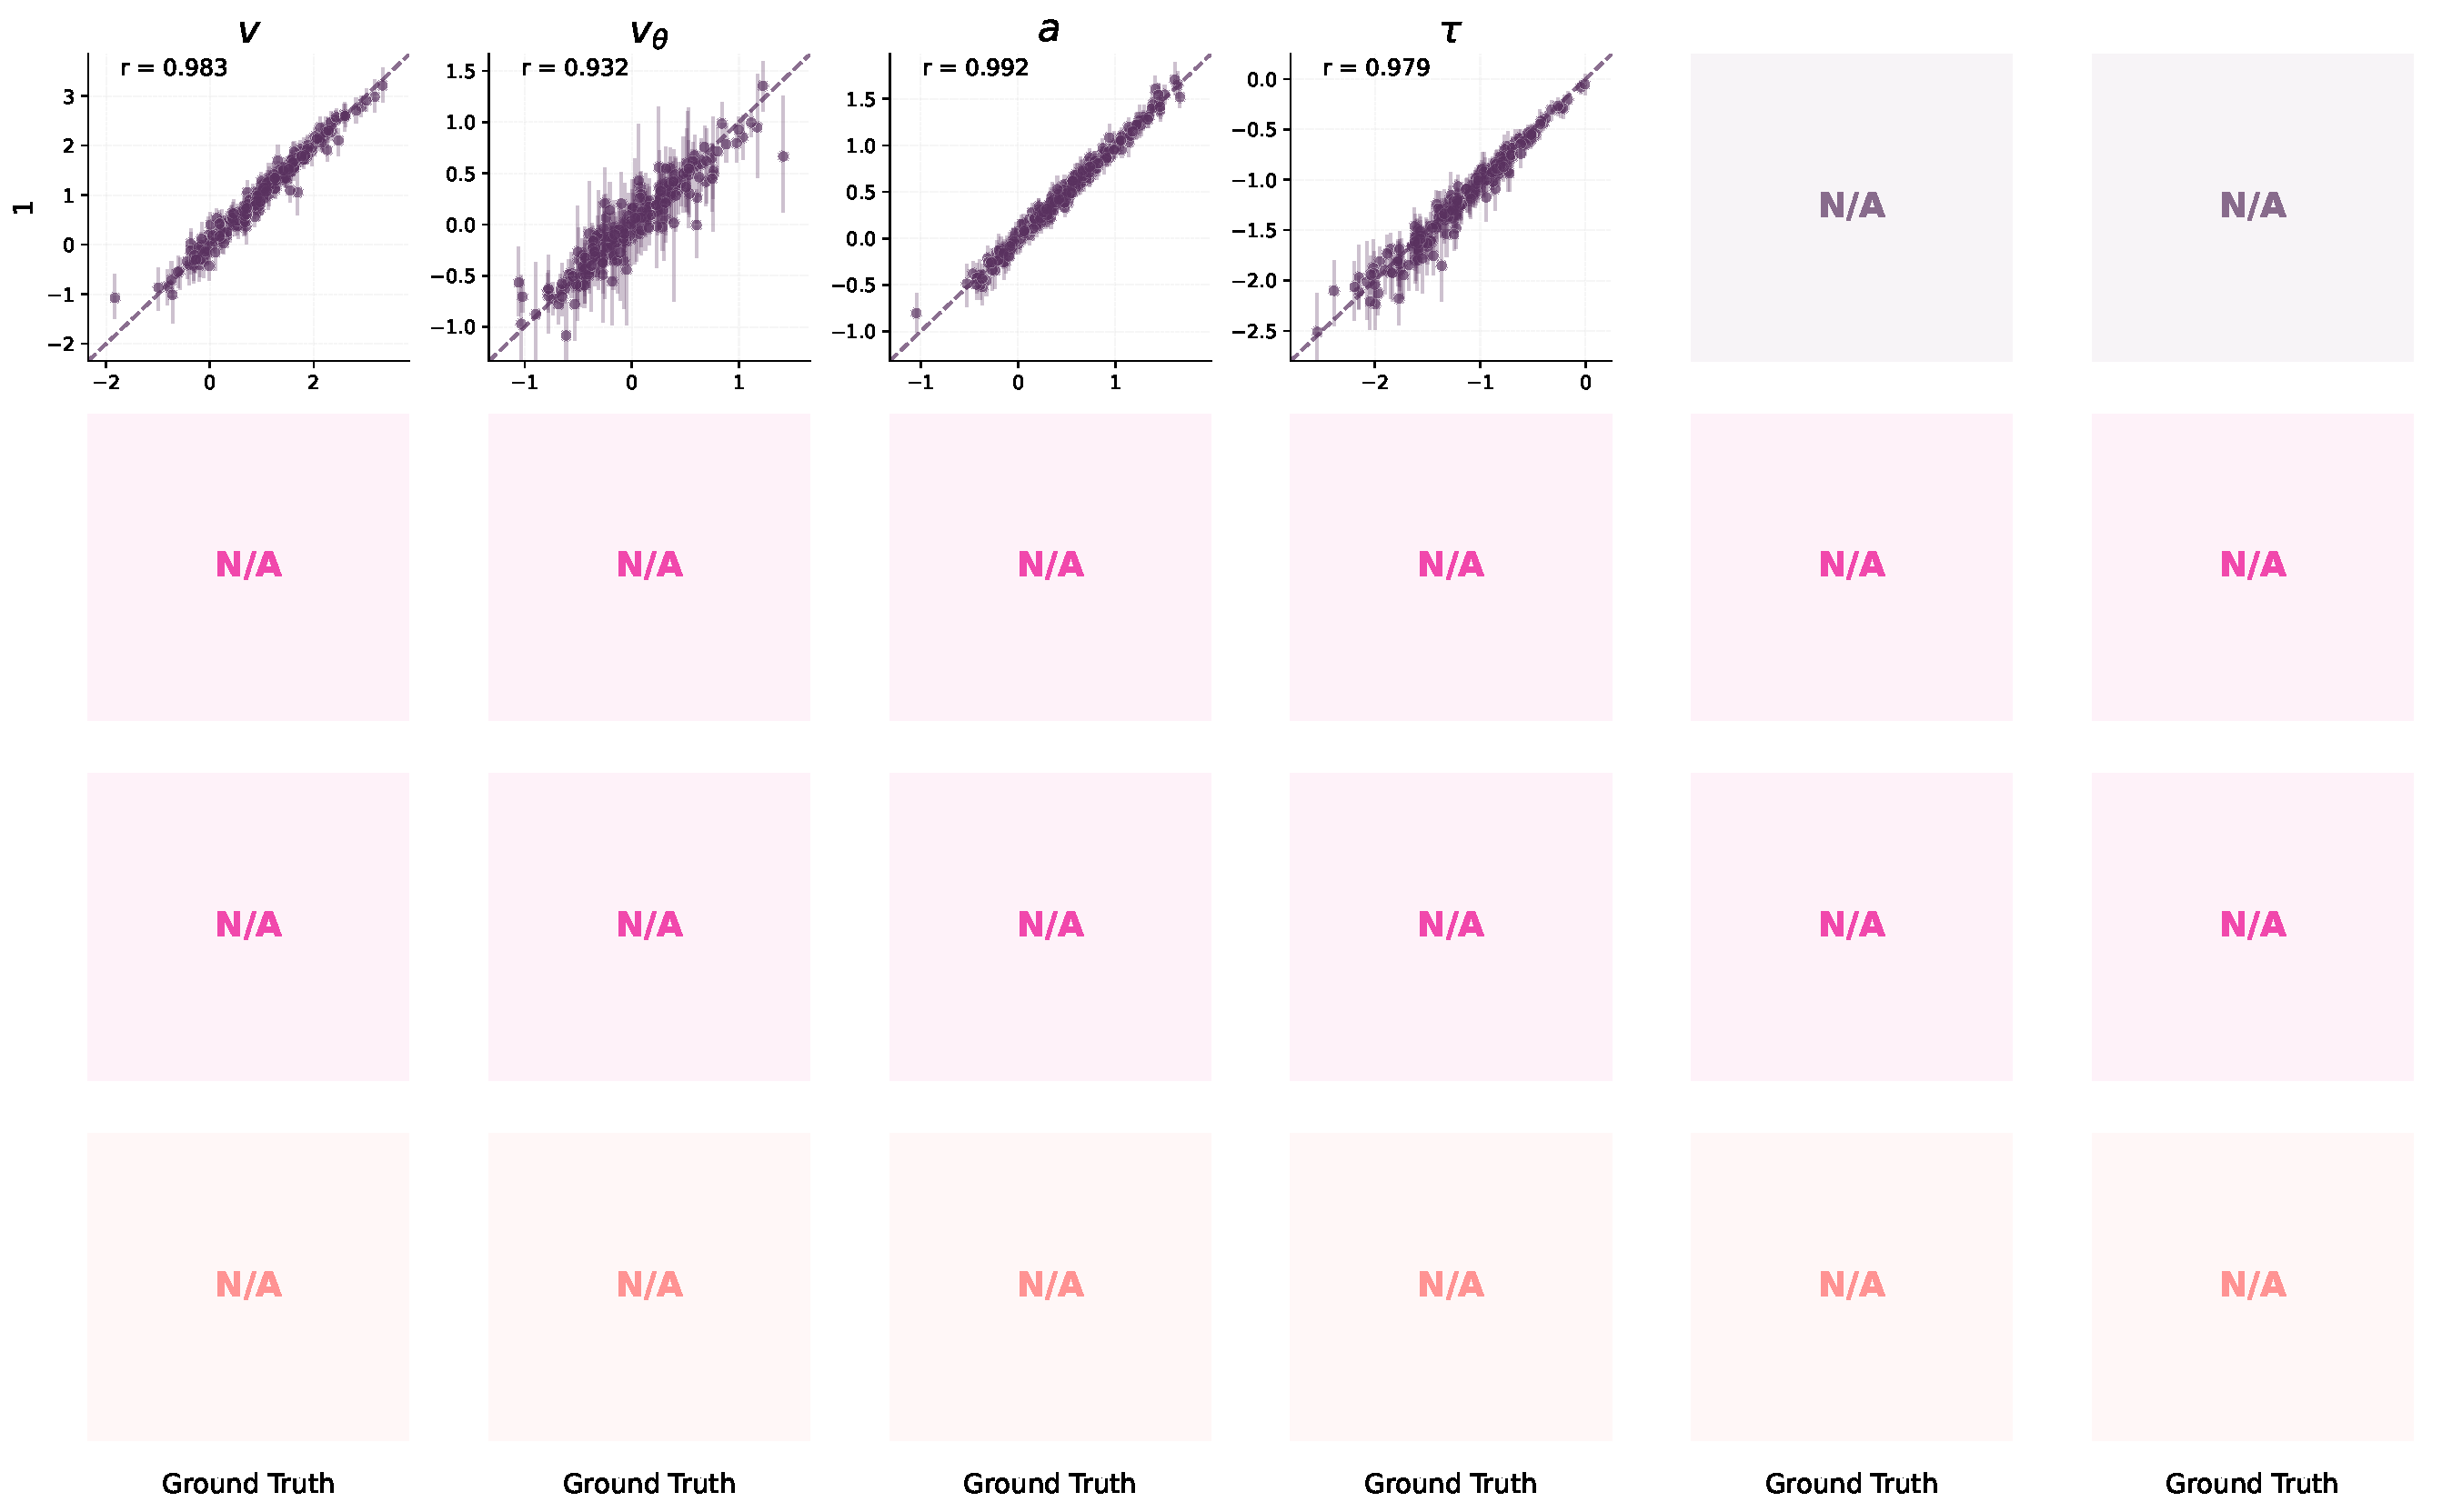
\includegraphics[width=0.99\linewidth]{figures/fm/cdm/fixed/cdm_family_fixed_fm_mixed_recovery.pdf}
    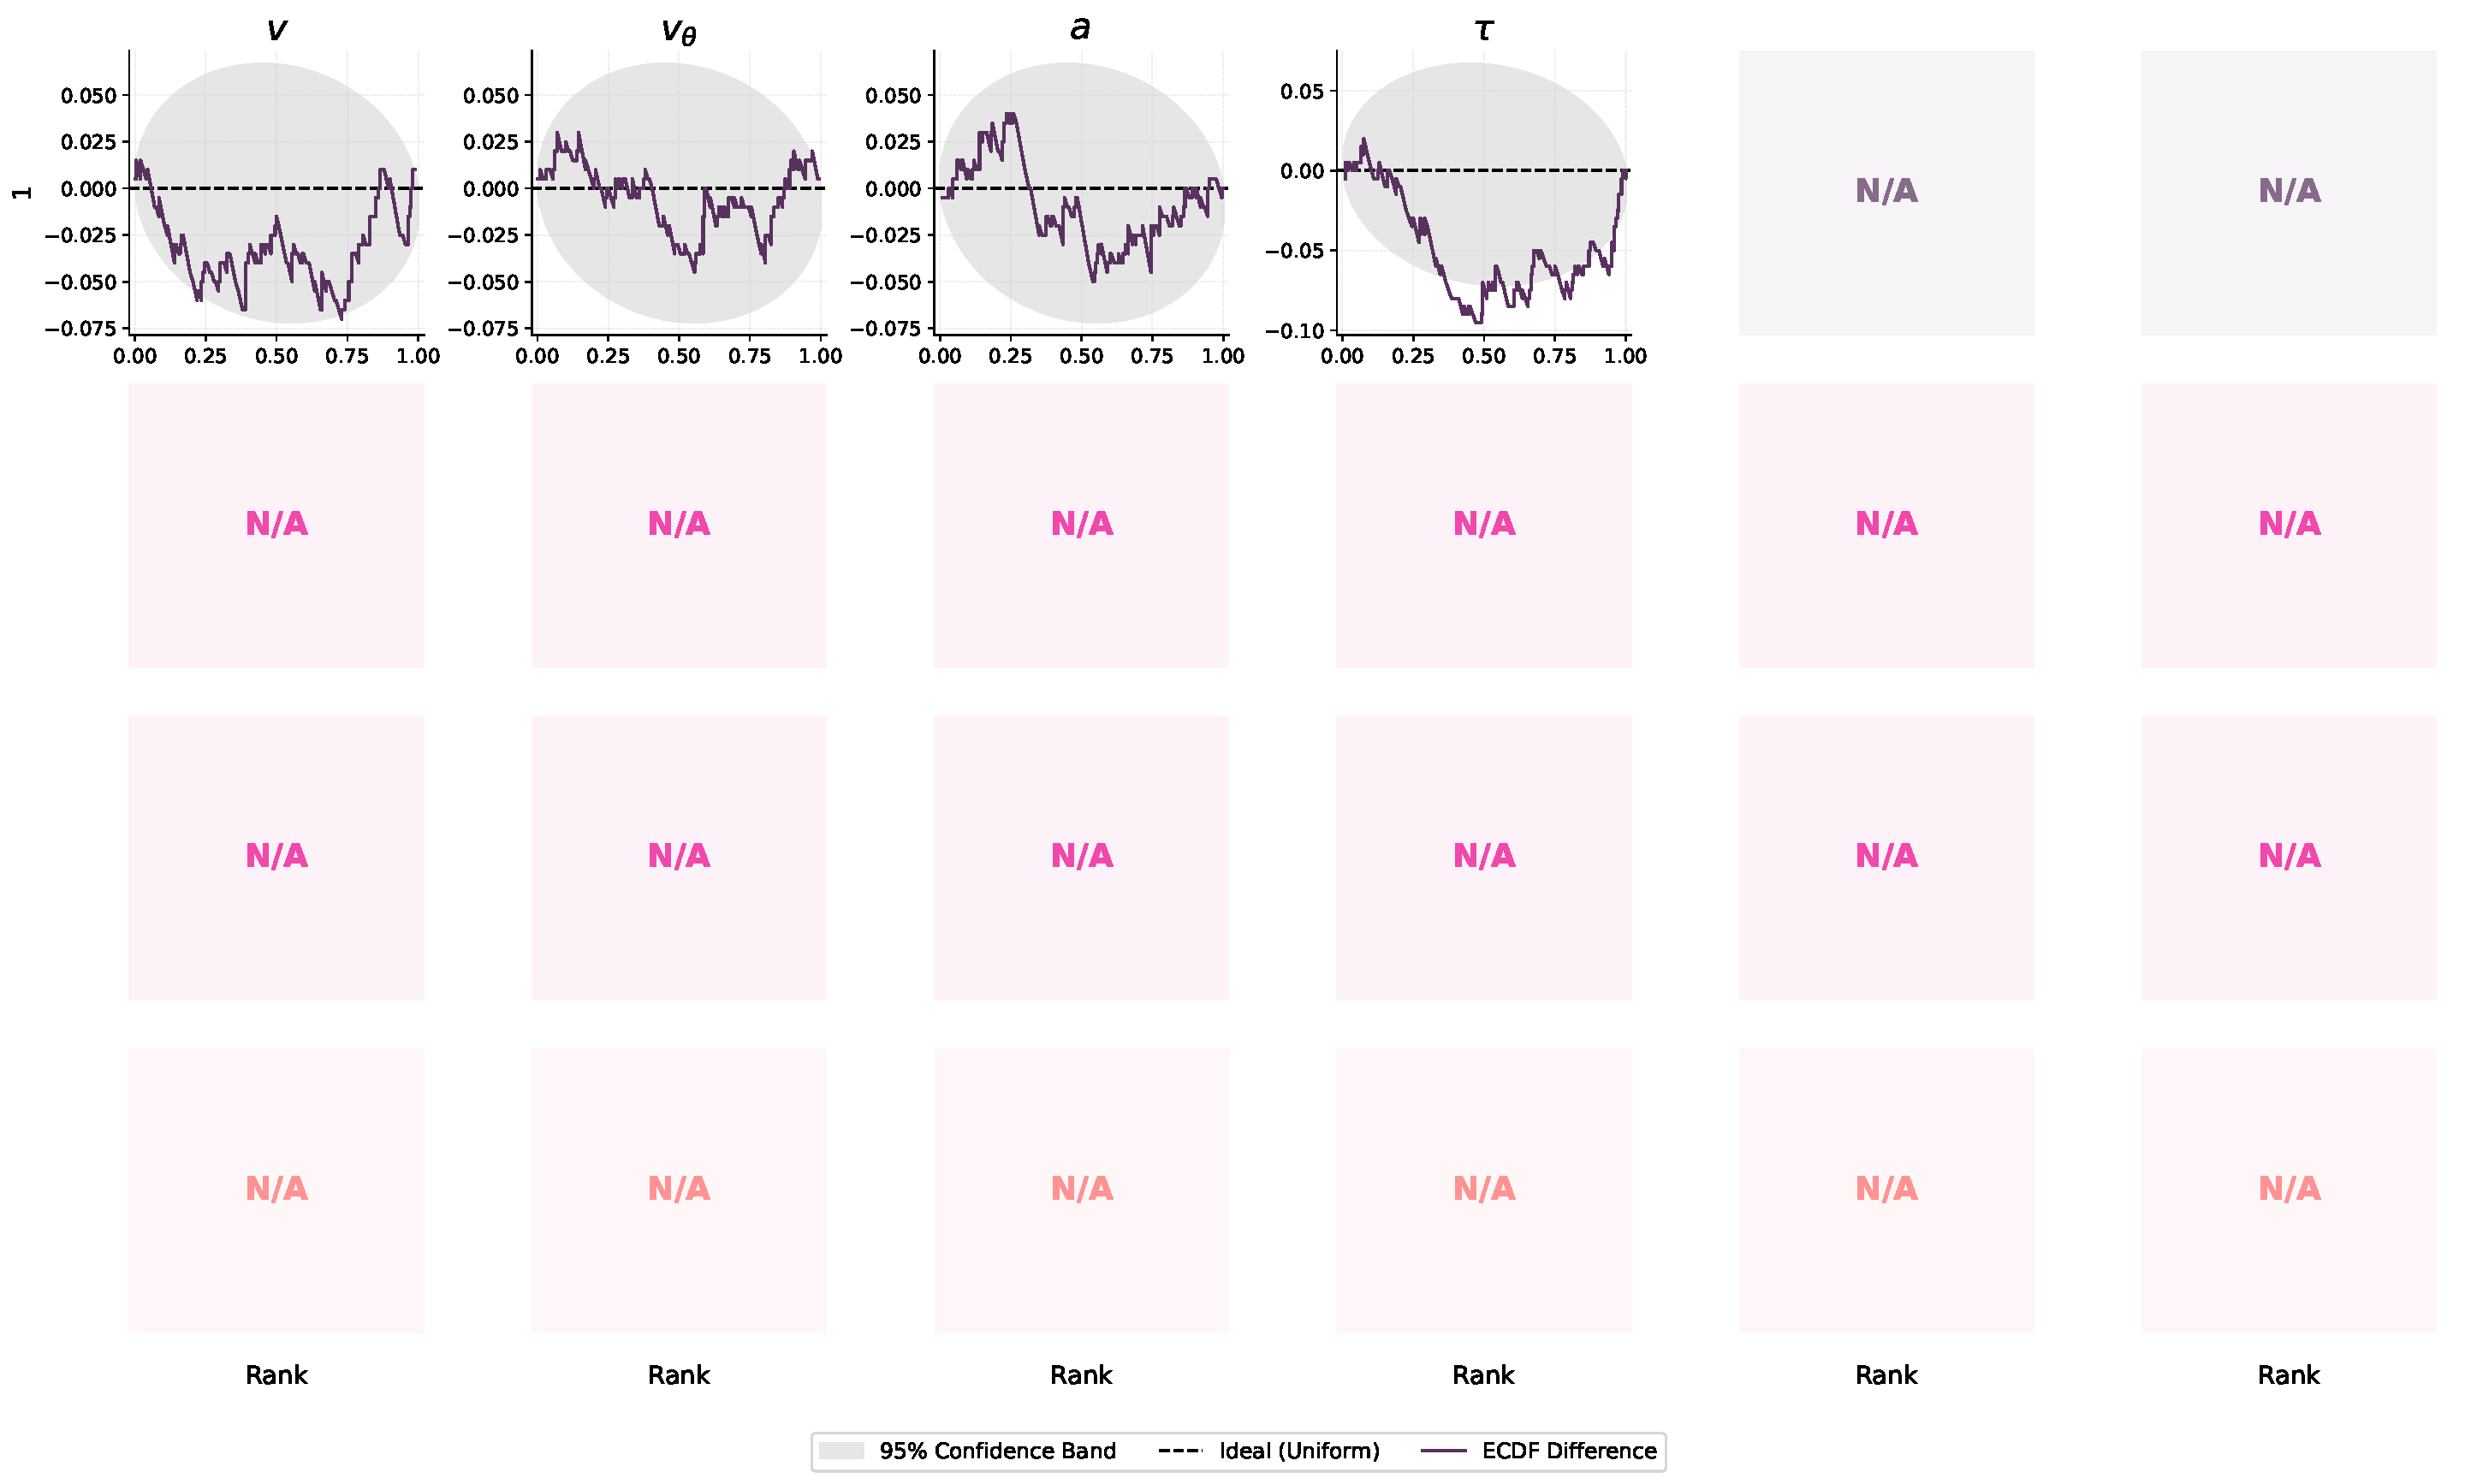
\includegraphics[width=0.99\linewidth]{figures/fm/cdm/fixed/cdm_family_fixed_fm_mixed_ecdf.pdf}
    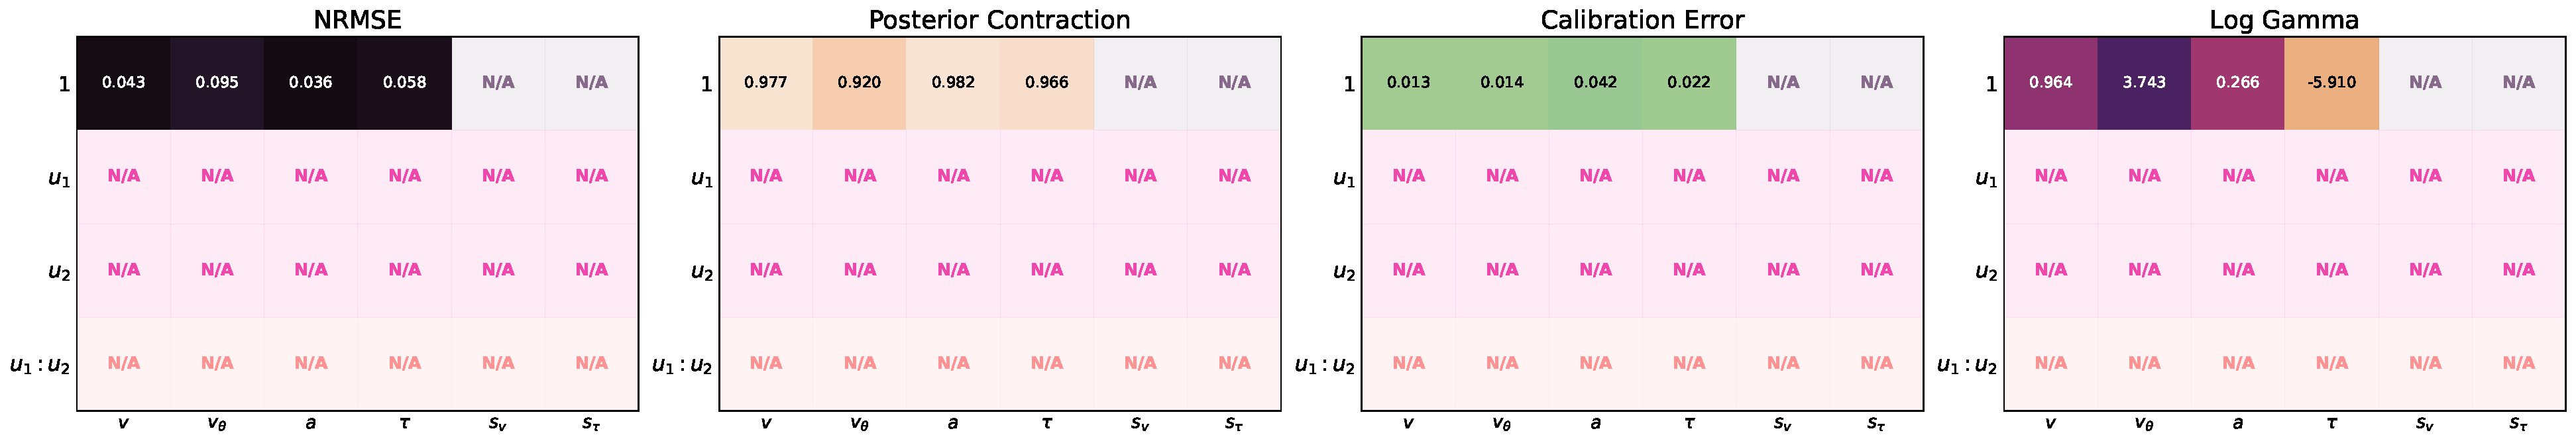
\includegraphics[width=0.99\linewidth]{figures/fm/cdm/fixed/cdm_family_fixed_fm_mixed_metrics.pdf}
    \caption{Parameter recovery (\emph{top}), calibration ECDF (\emph{middle}), and parameter-wise metrics (NRMSE, calibration error, and posterior contraction) for CDM model family (Case \textbf{fixed}).}
    \label{fig:cdm-fm-fixed}
\end{figure}

\begin{figure}
    \centering
    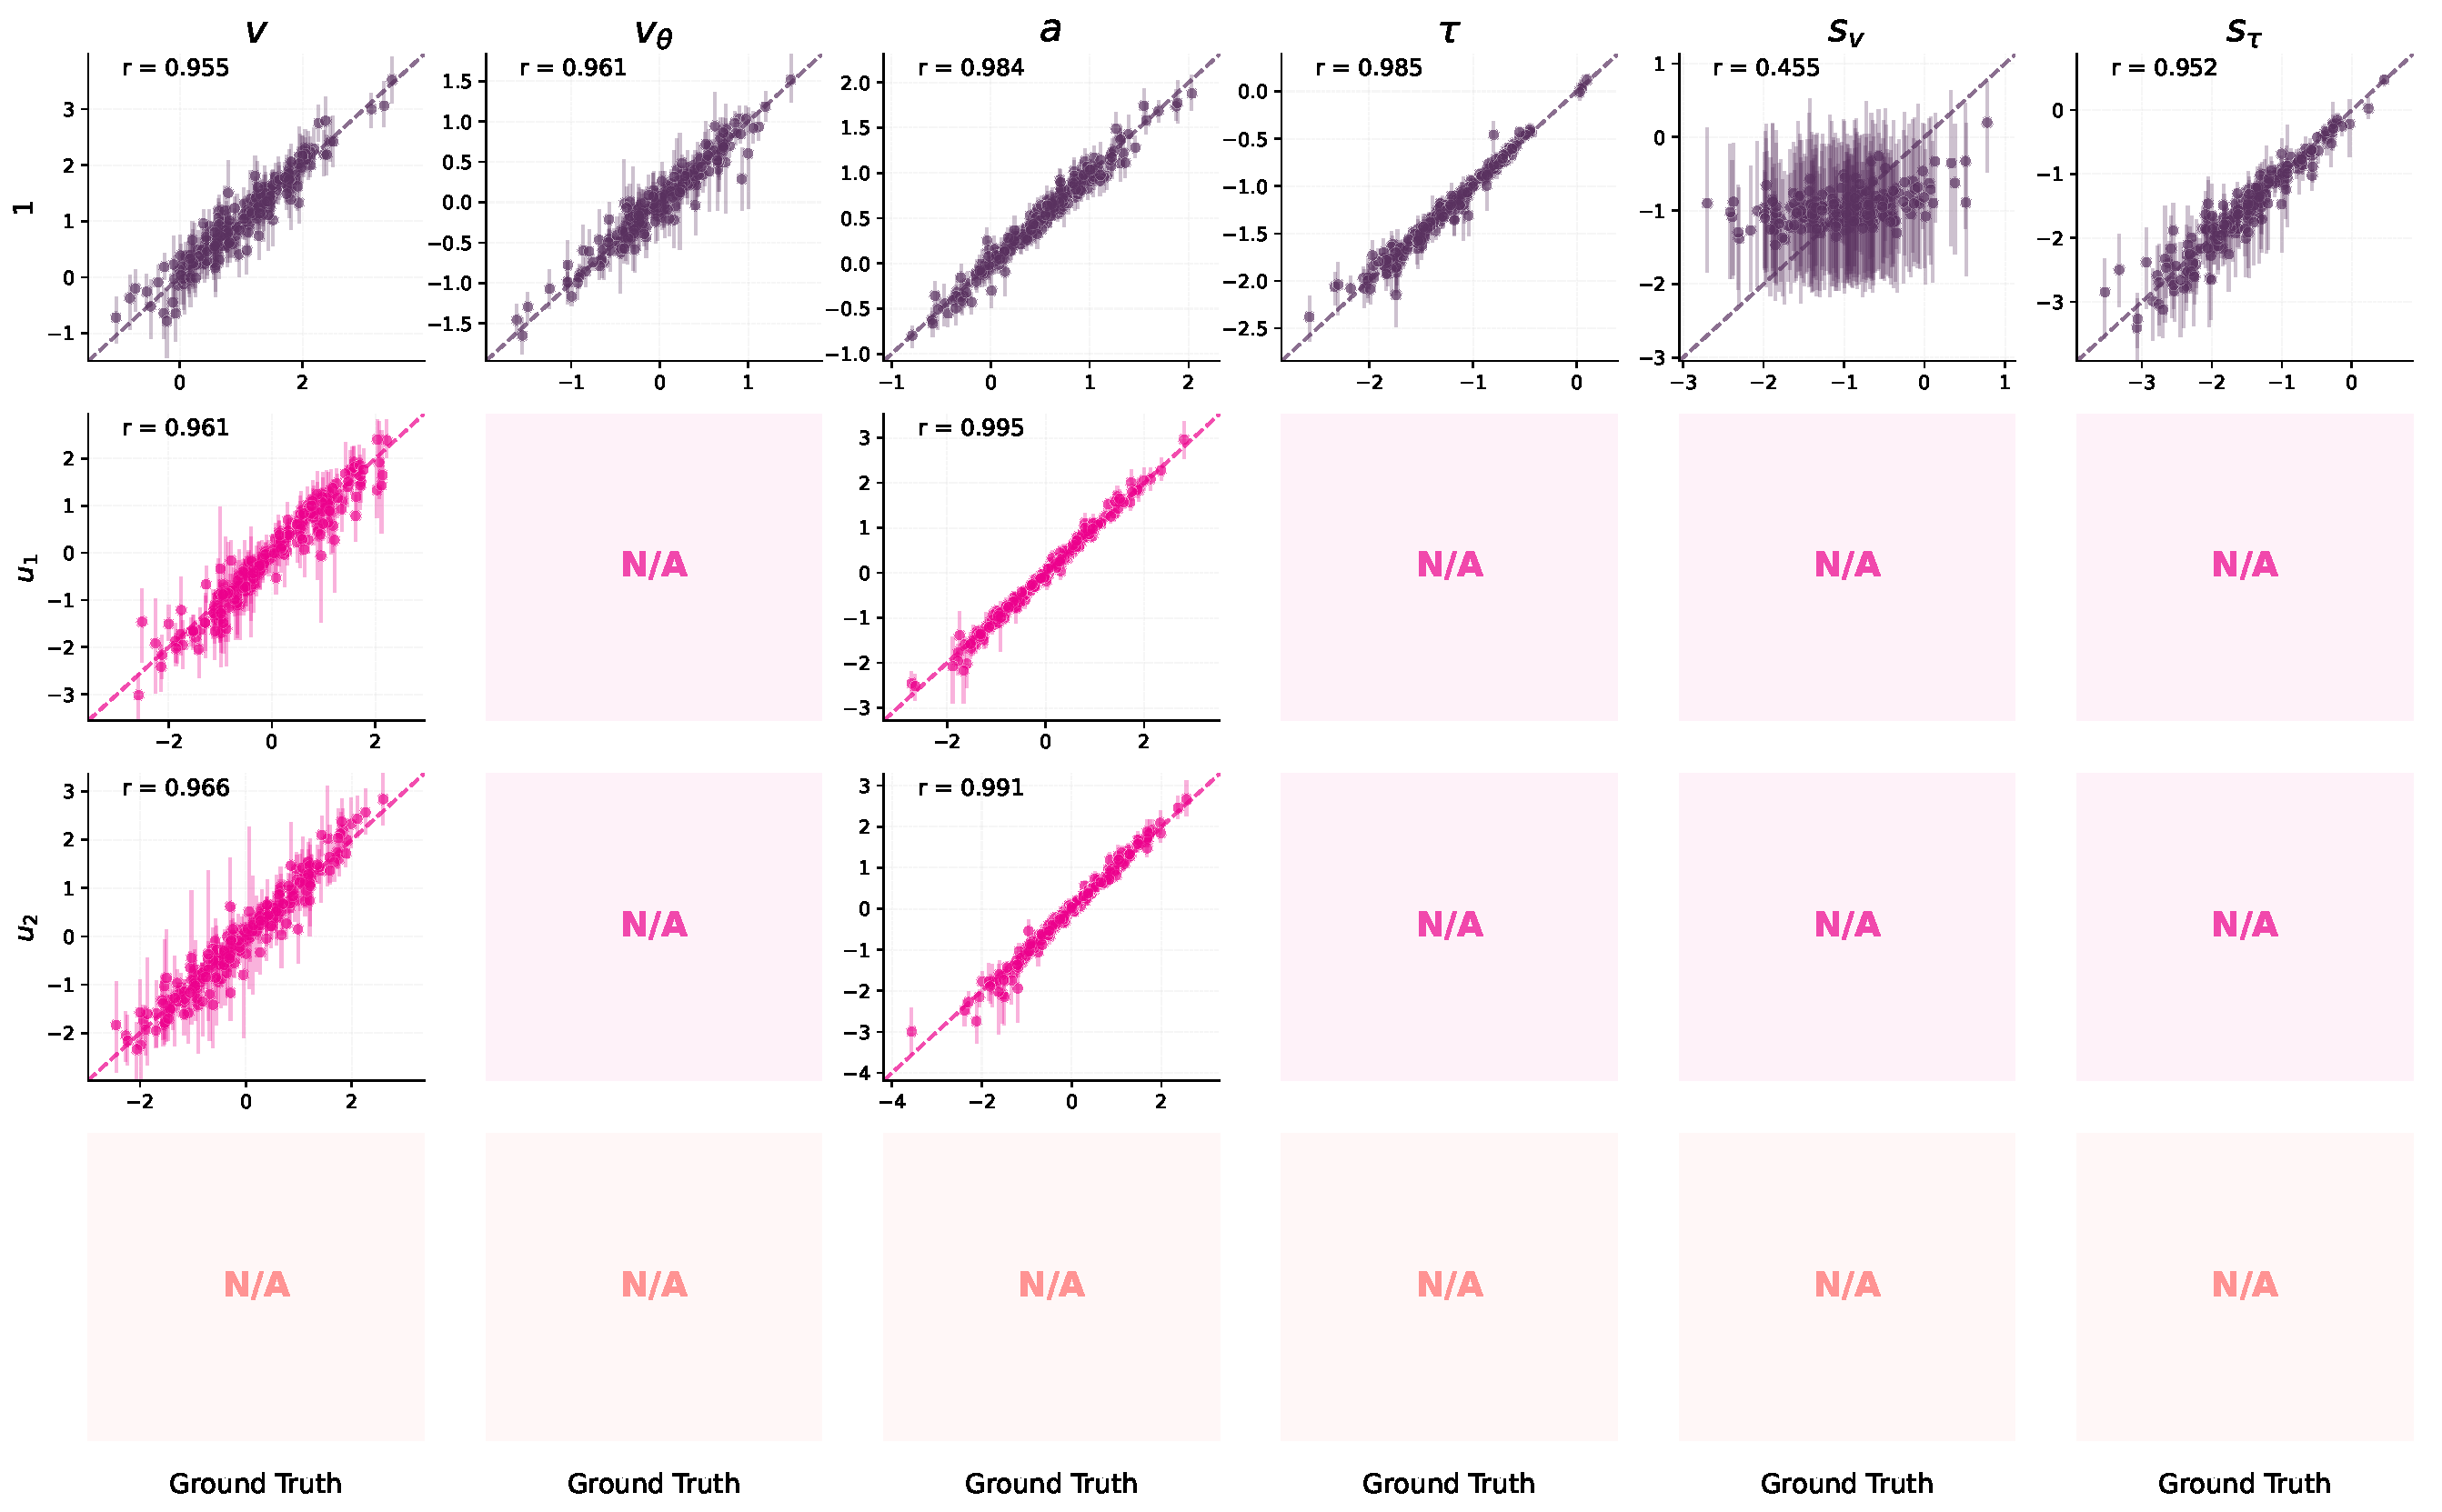
\includegraphics[width=0.99\linewidth]{figures/fm/cdm/regressed/cdm_family_regressed_fm_mixed_recovery.pdf}
    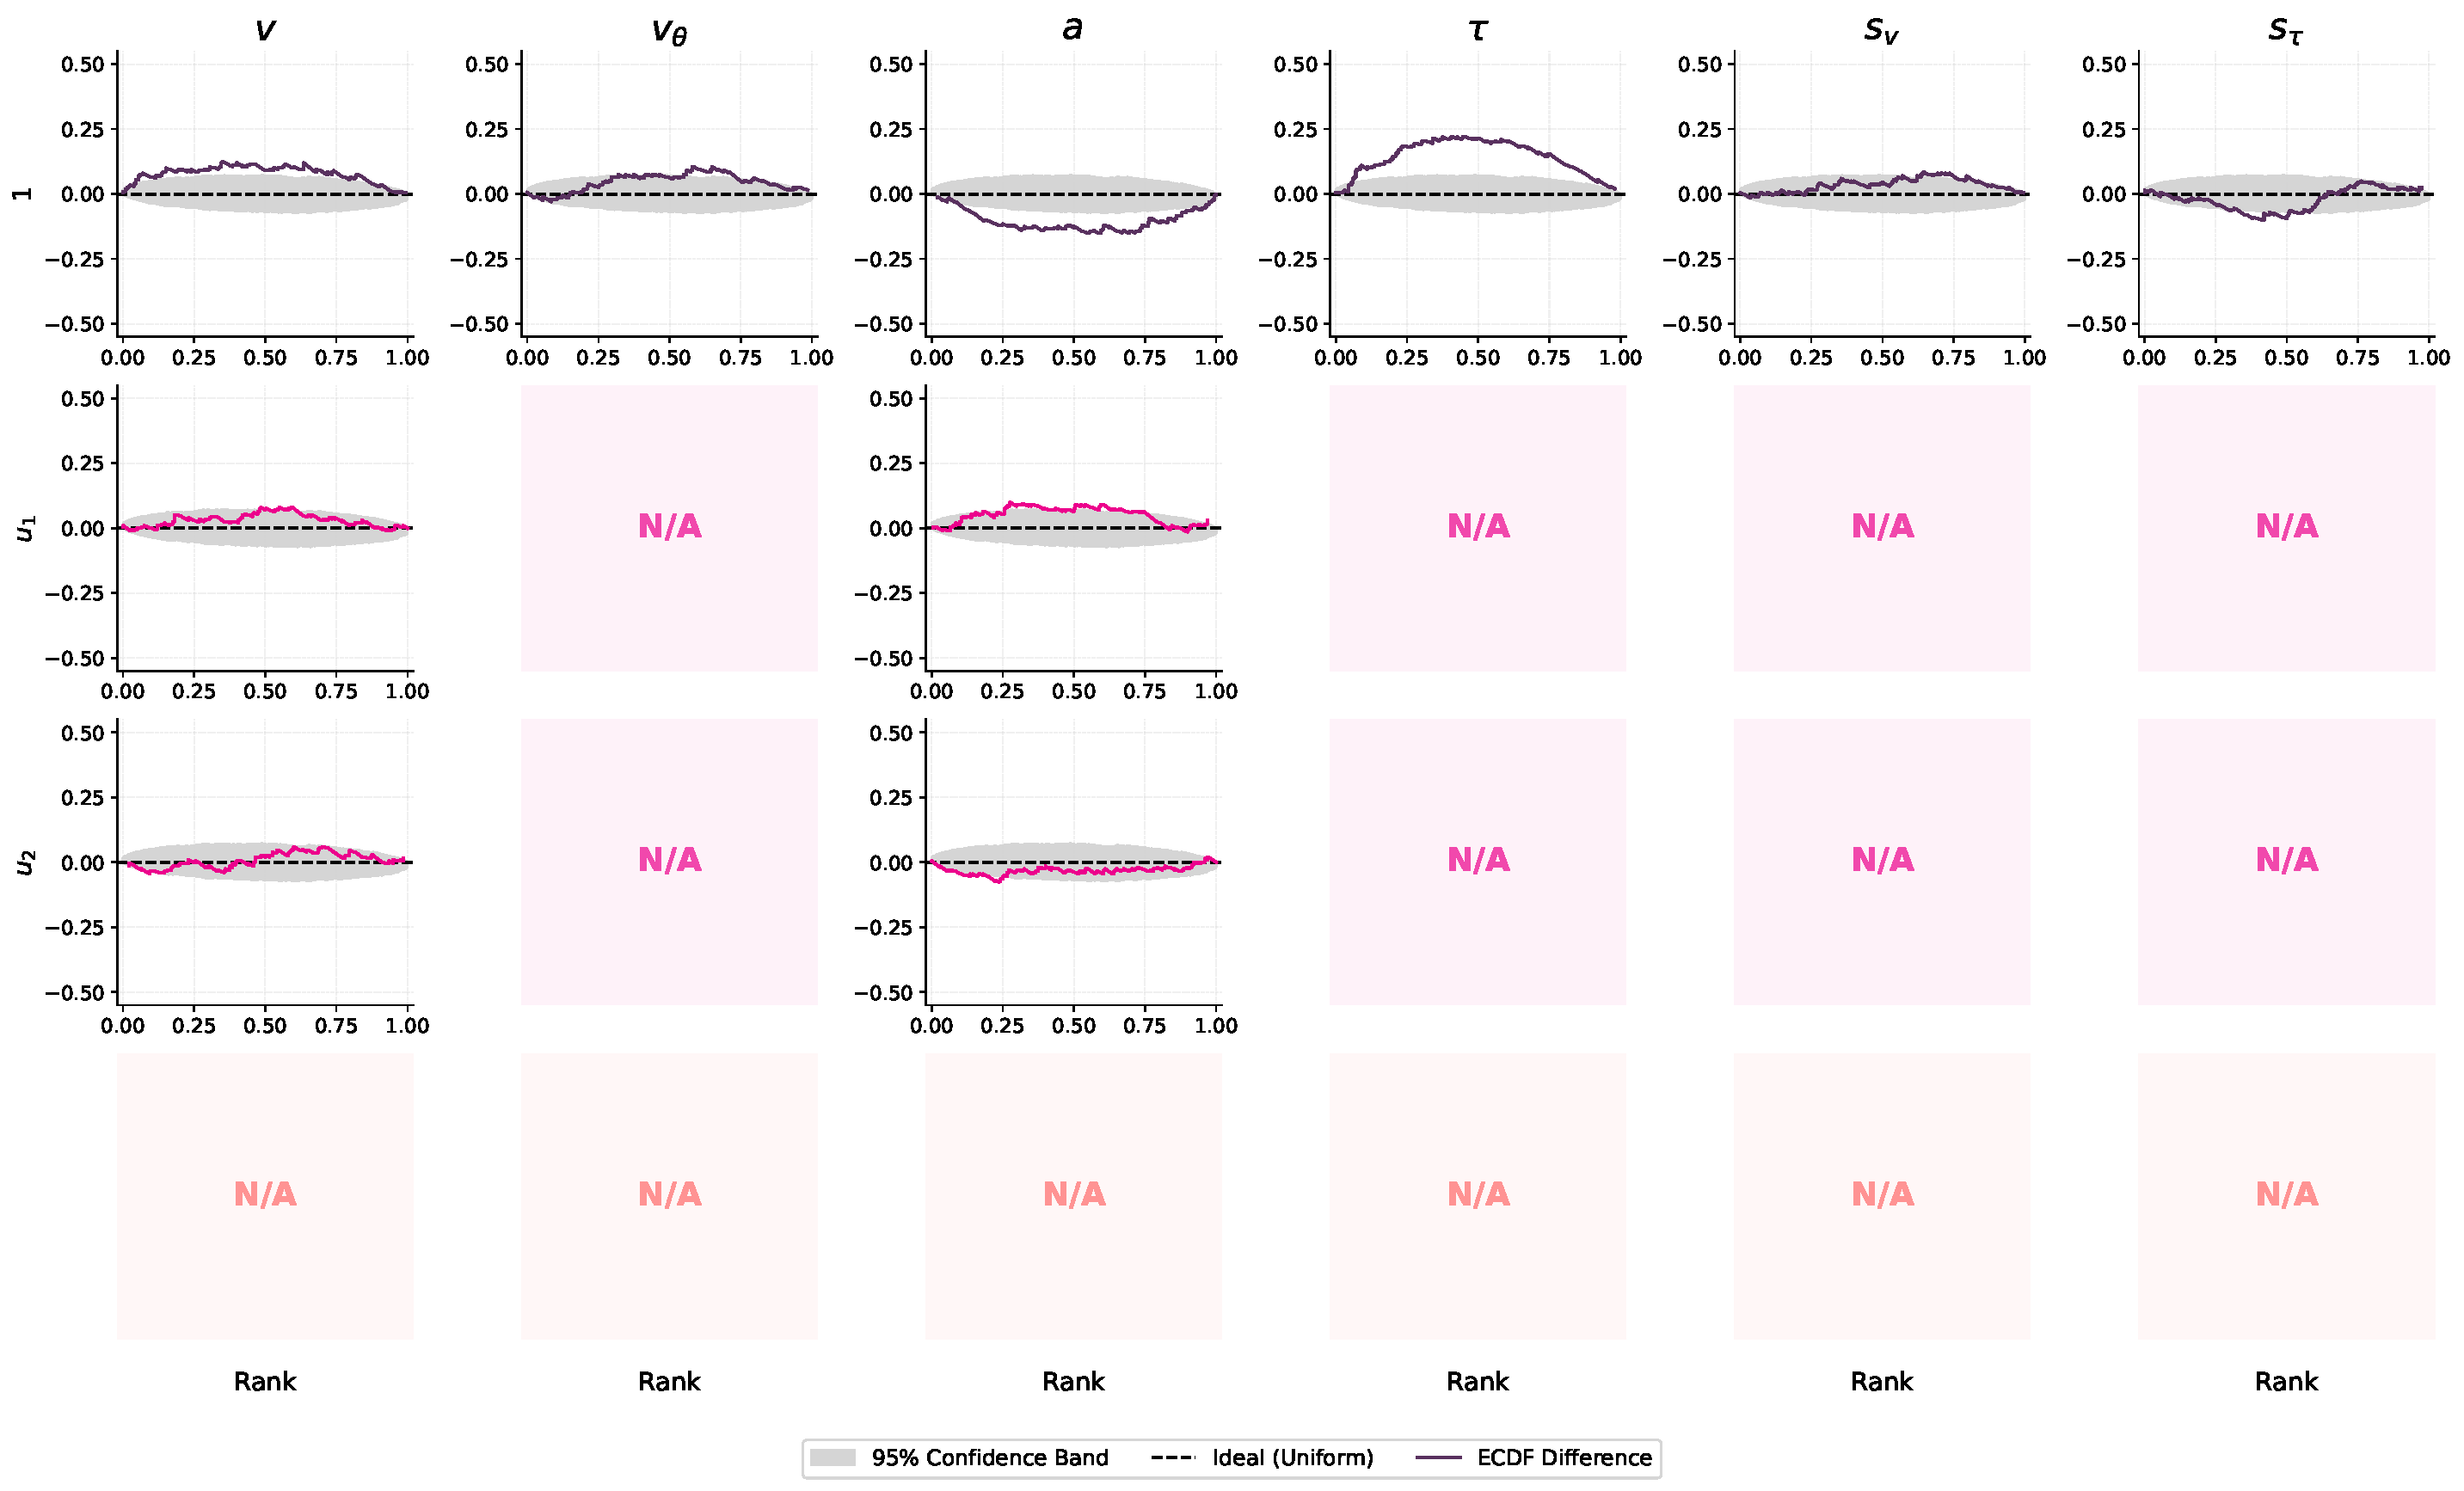
\includegraphics[width=0.99\linewidth]{figures/fm/cdm/regressed/cdm_family_regressed_fm_mixed_ecdf.pdf}
    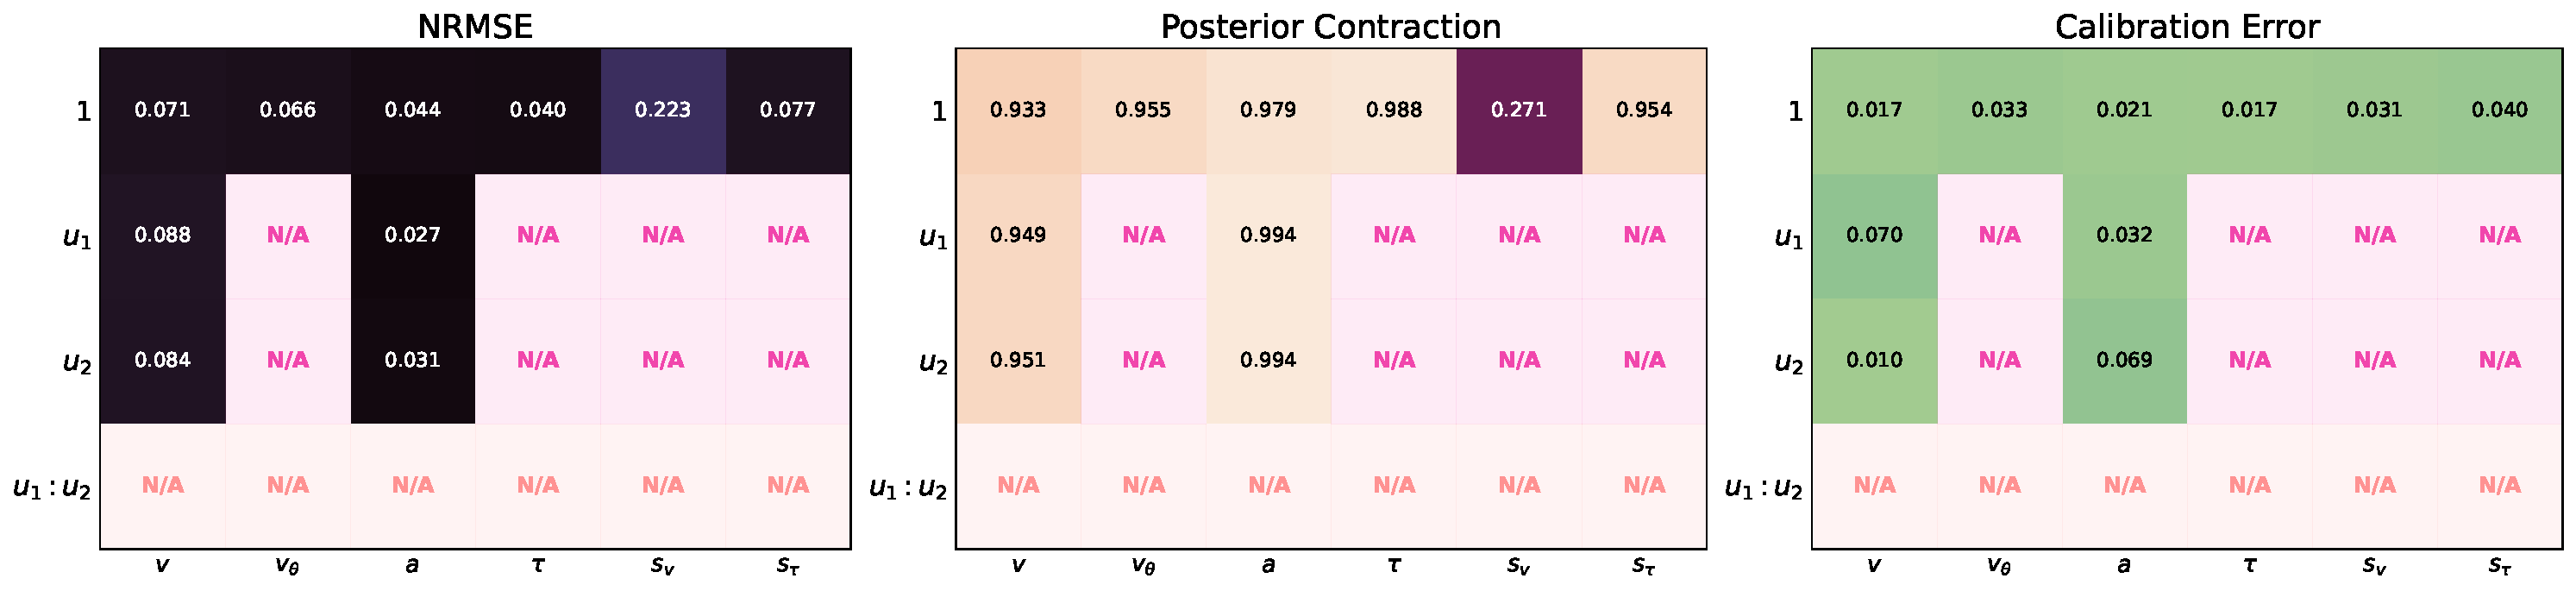
\includegraphics[width=0.99\linewidth]{figures/fm/cdm/regressed/cdm_family_regressed_fm_mixed_metrics.pdf}
    \caption{Parameter recovery (\emph{top}), calibration ECDF (\emph{middle}), and parameter-wise metrics (NRMSE, calibration error, and posterior contraction) for CDM model family (Case \textbf{regressed}).}
    \label{fig:cdm-fm-regressed}
\end{figure}

\begin{figure}
    \centering
    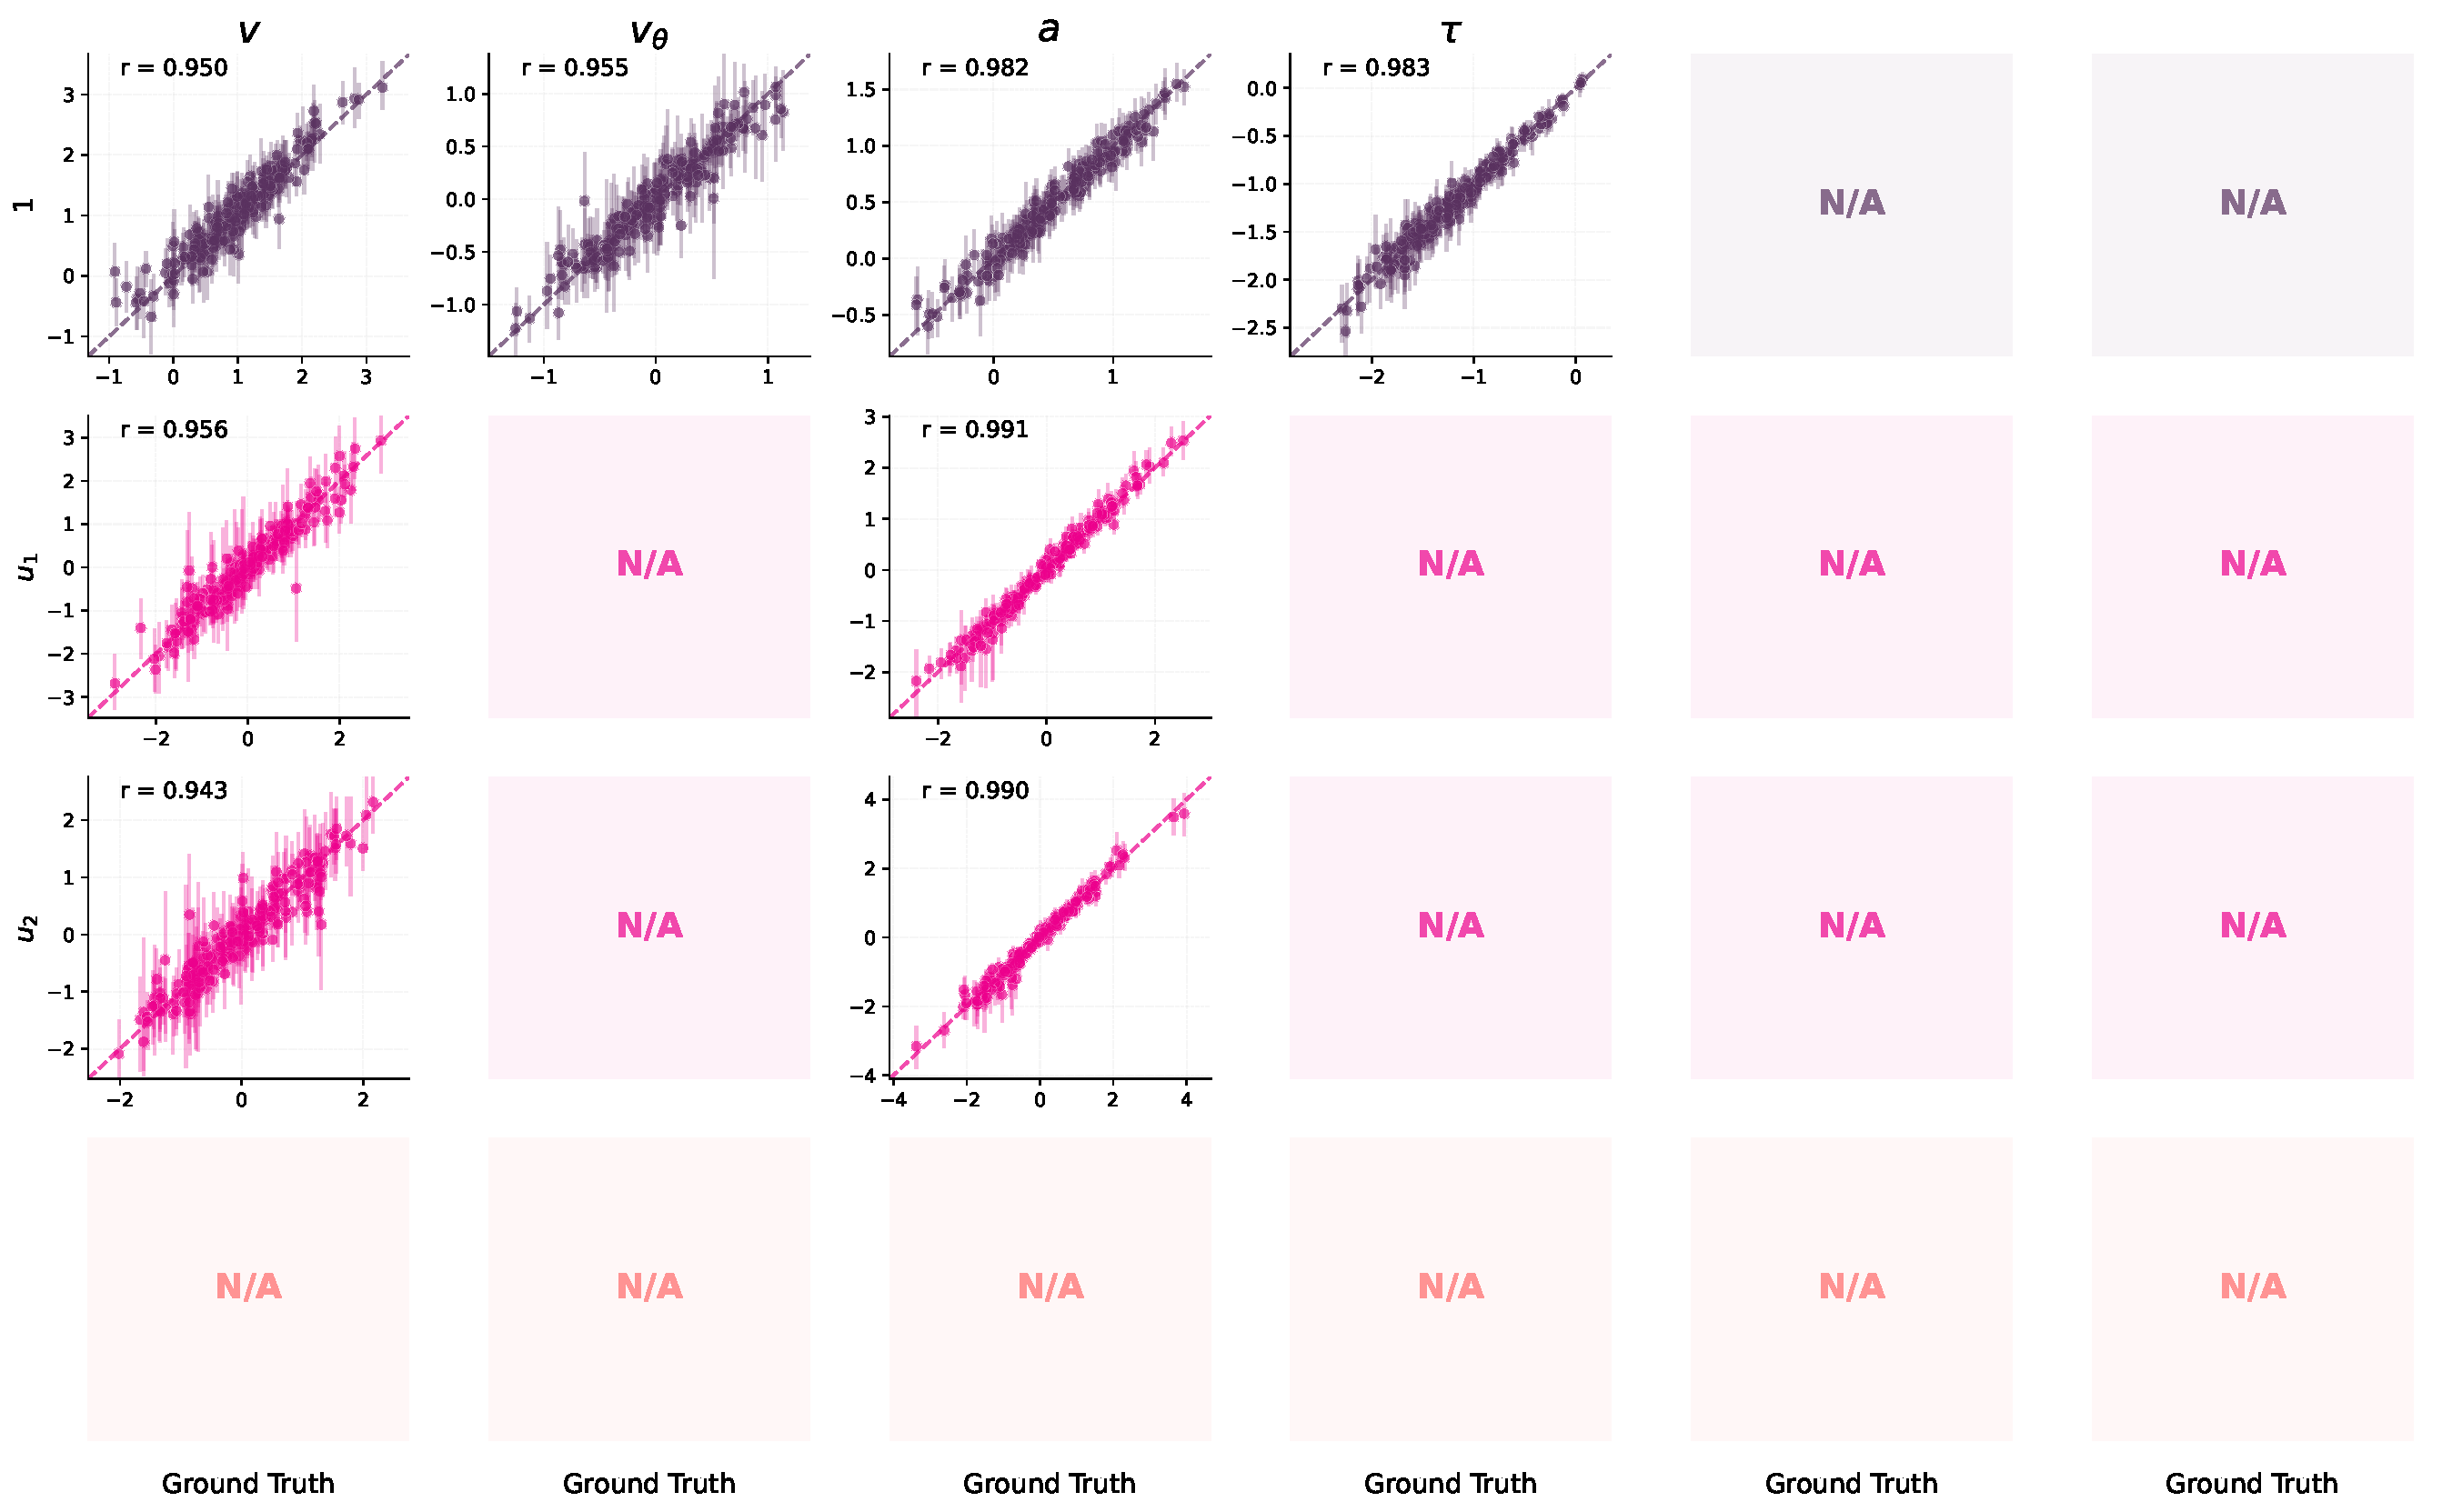
\includegraphics[width=0.99\linewidth]{figures/fm/cdm/fixed_regressed/cdm_family_fixed_regressed_fm_mixed_recovery.pdf}
    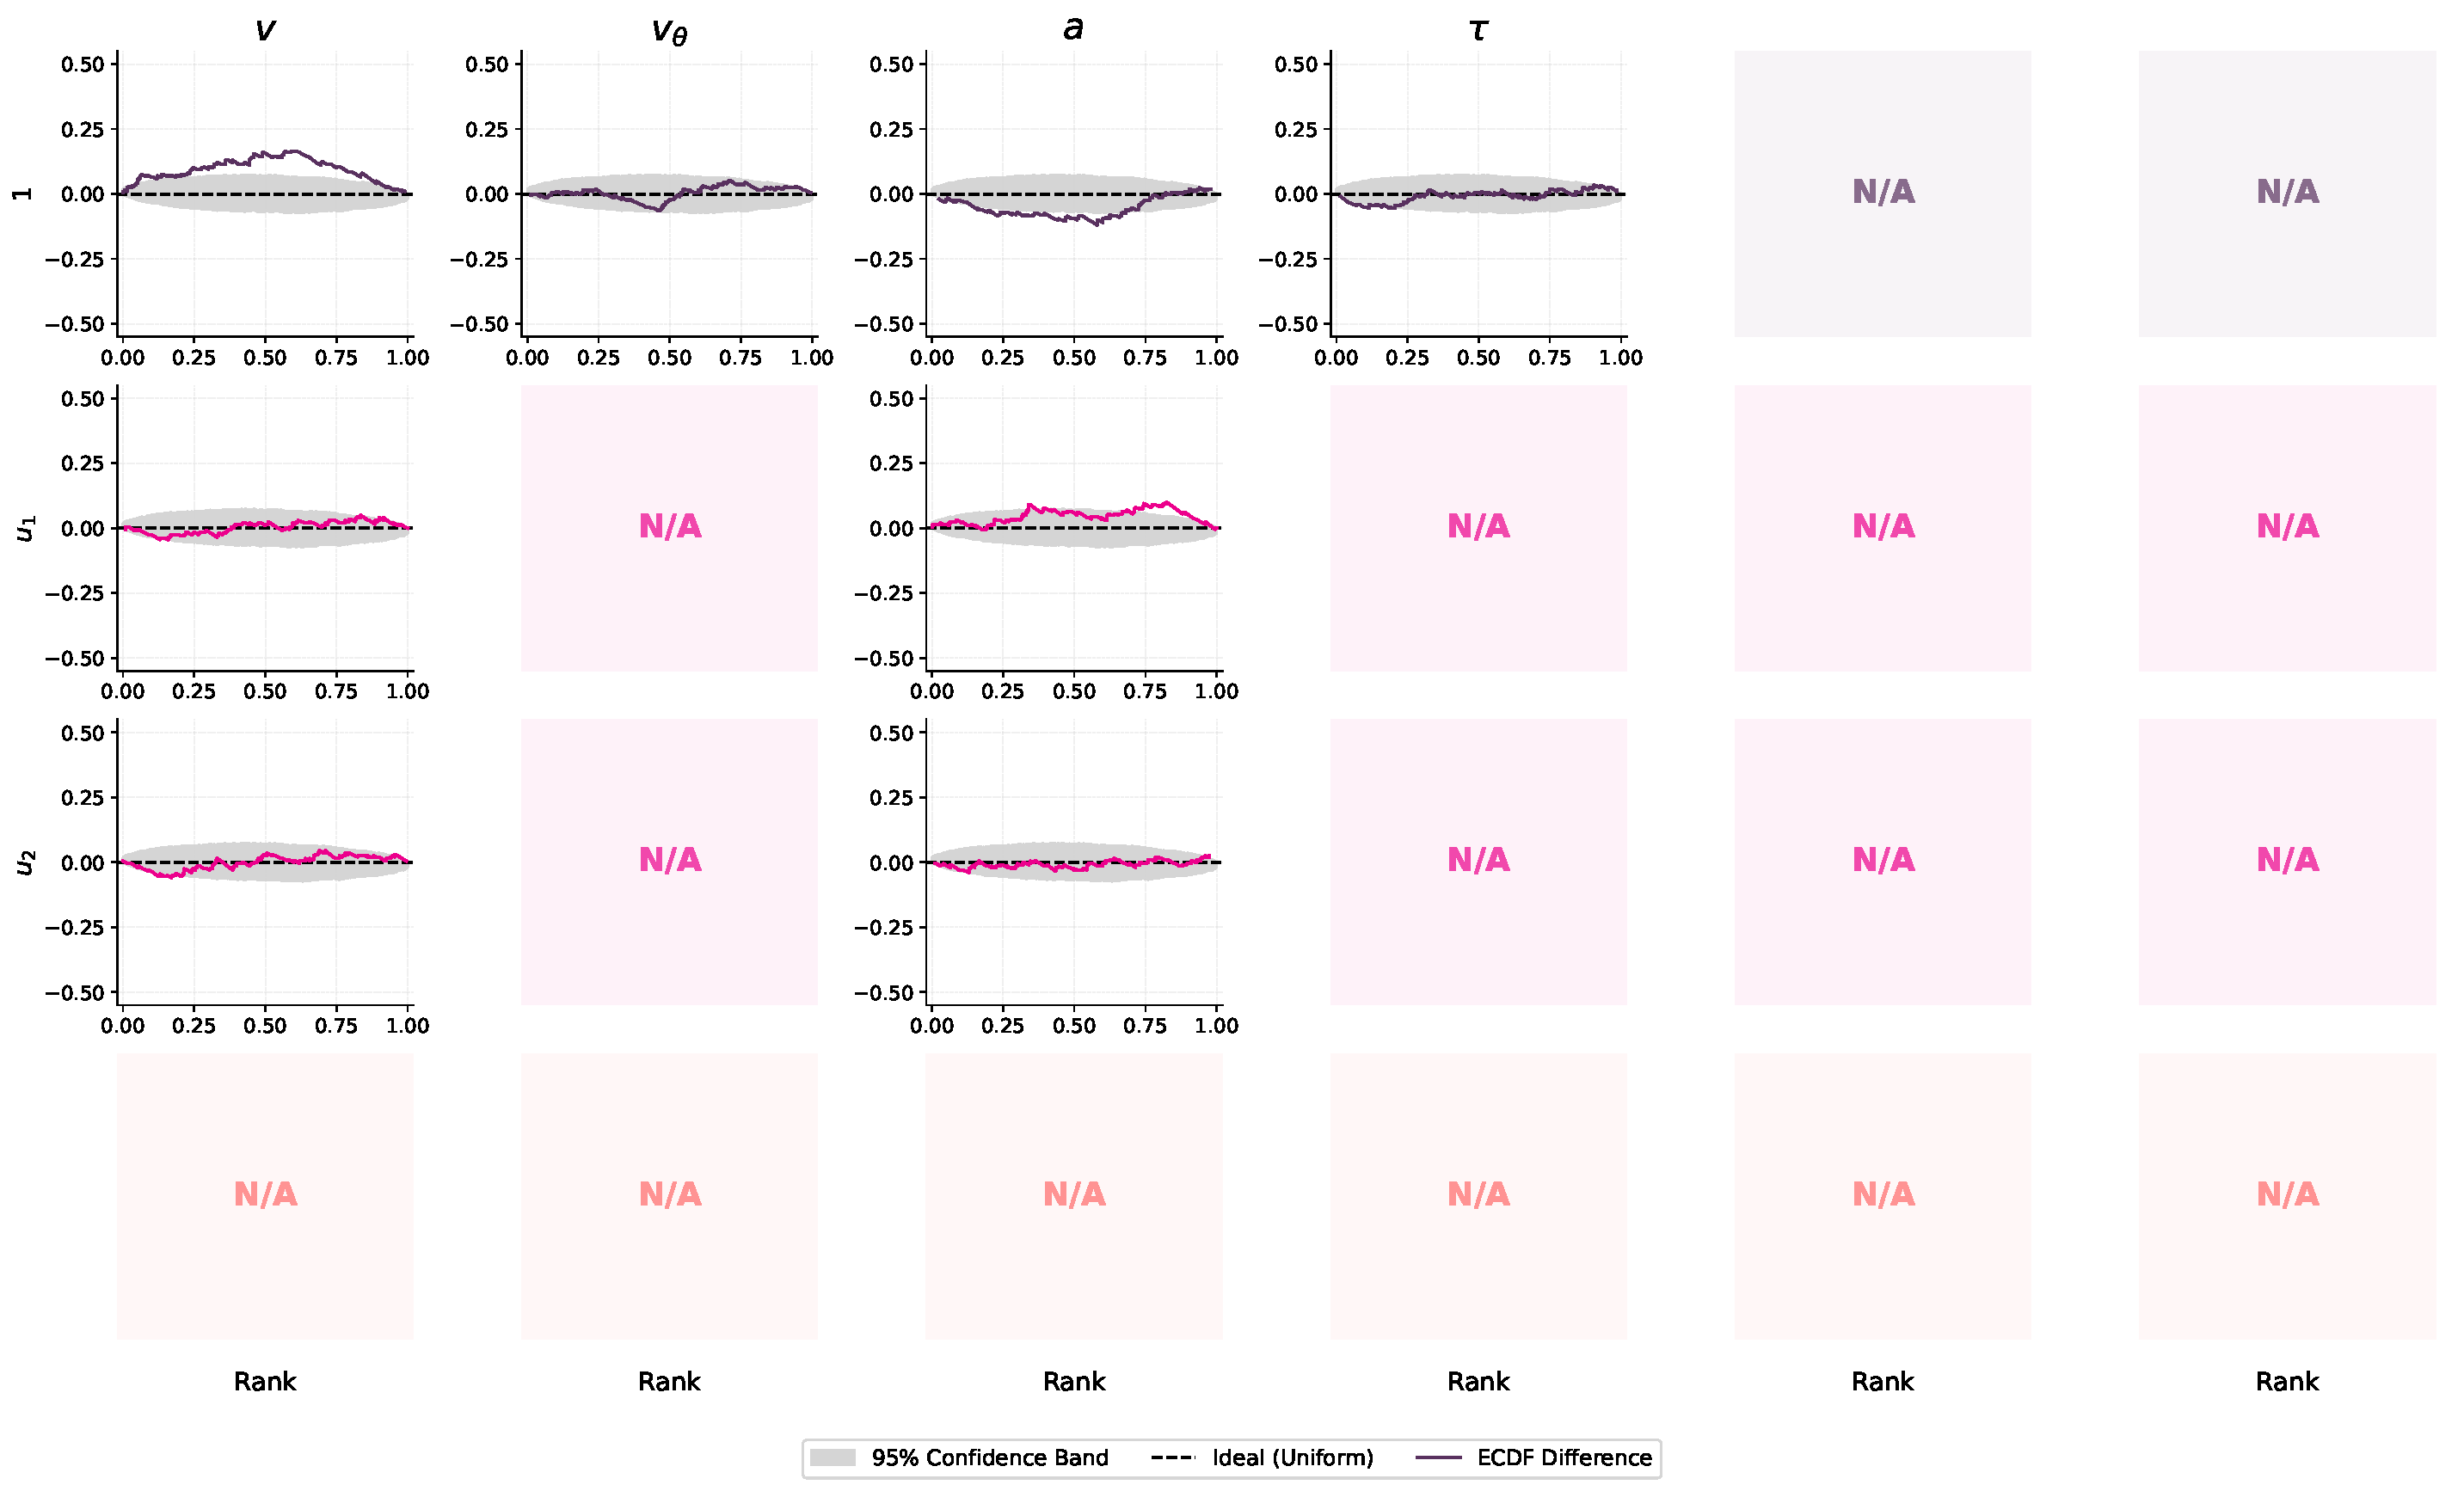
\includegraphics[width=0.99\linewidth]{figures/fm/cdm/fixed_regressed/cdm_family_fixed_regressed_fm_mixed_ecdf.pdf}
    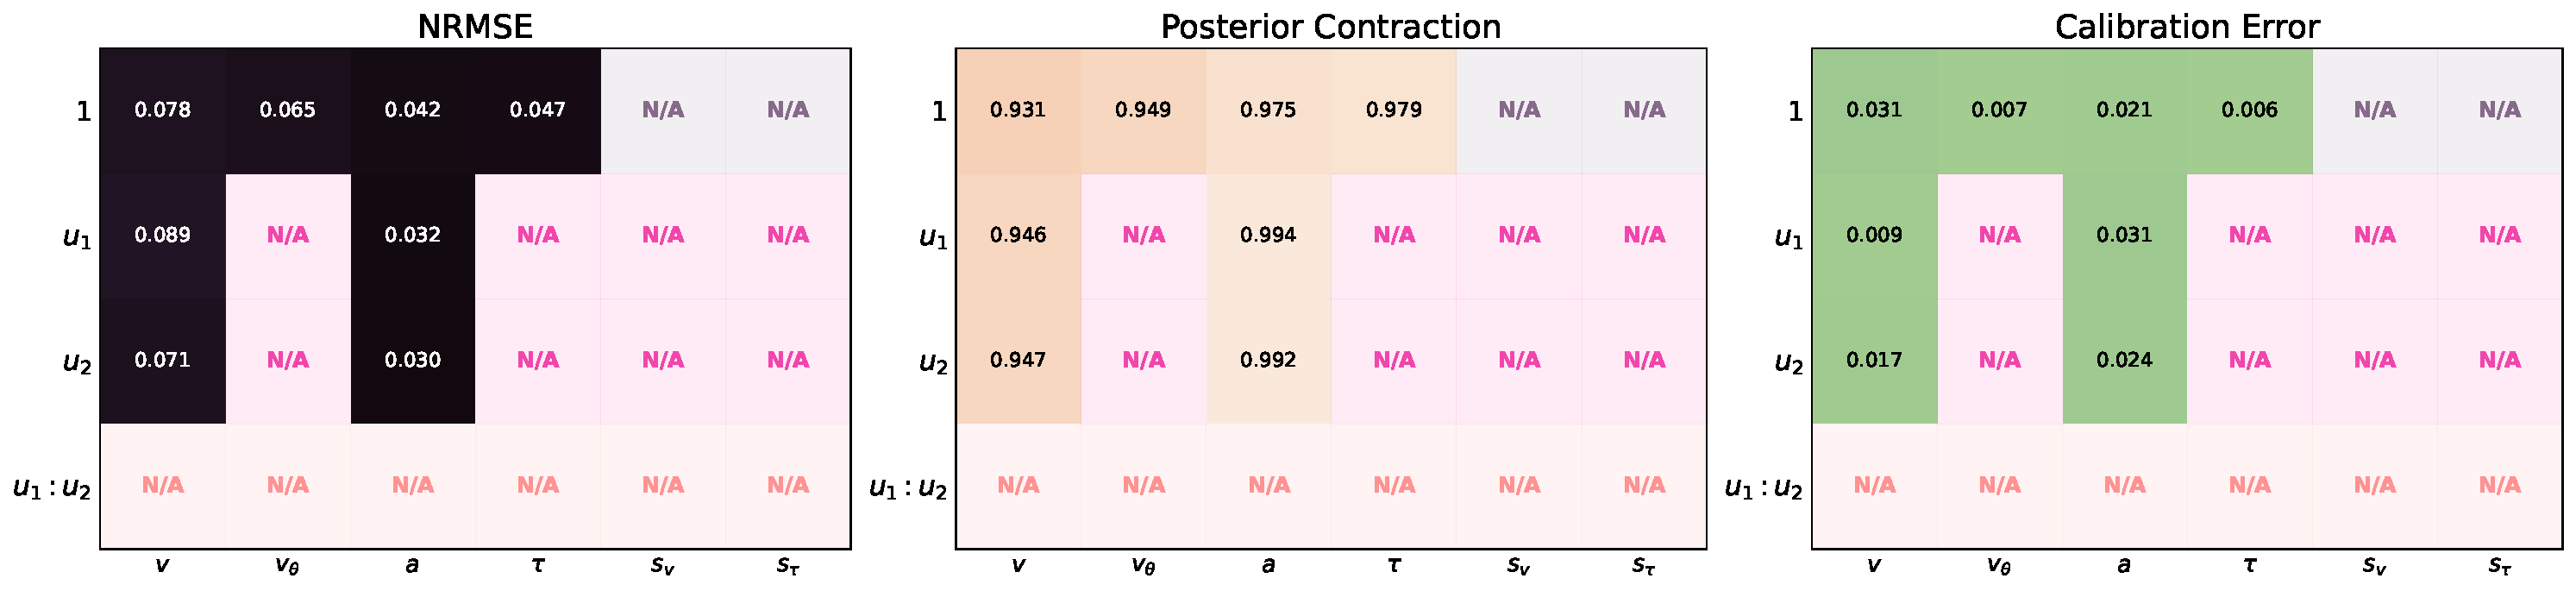
\includegraphics[width=0.99\linewidth]{figures/fm/cdm/fixed_regressed/cdm_family_fixed_regressed_fm_mixed_metrics.pdf}
    \caption{Parameter recovery (\emph{top}), calibration ECDF (\emph{middle}), and parameter-wise metrics (NRMSE, calibration error, and posterior contraction) for CDM model family (Case \textbf{fixed\_regressed}).}
    \label{fig:cdm-fm-fixed-regressed}
\end{figure}

\begin{figure}
    \centering
    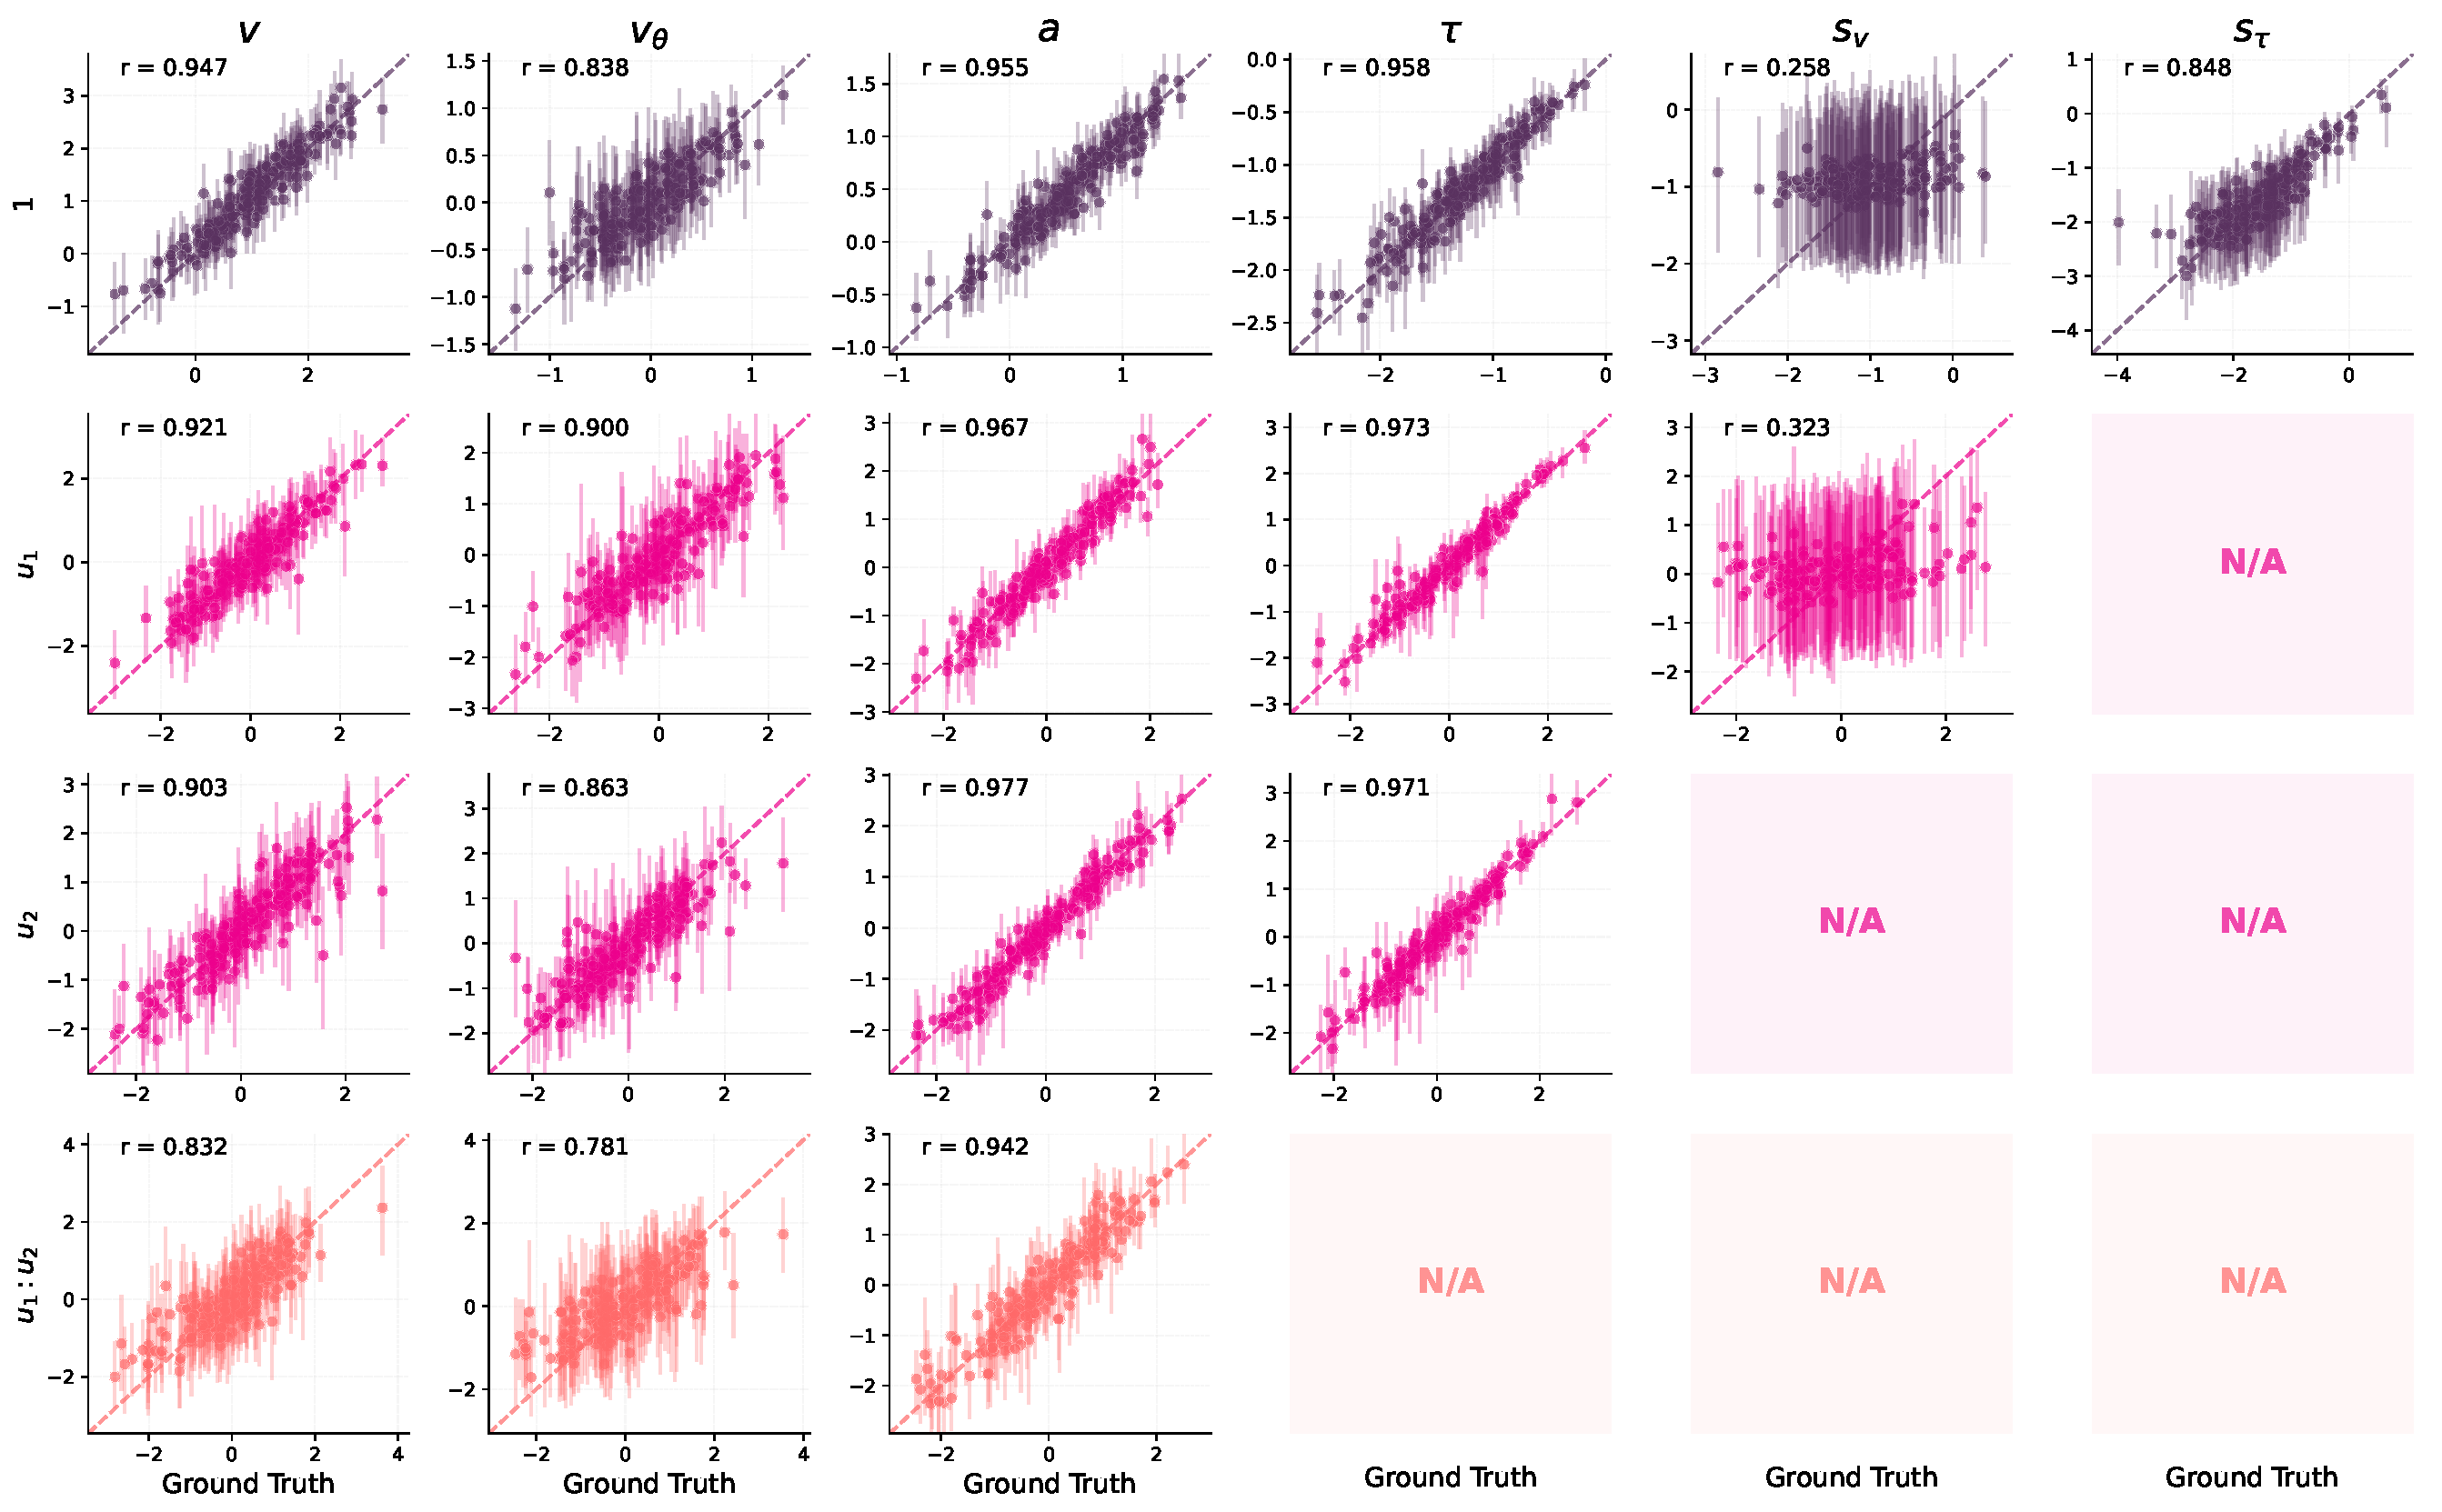
\includegraphics[width=0.99\linewidth]{figures/fm/cdm/interaction/cdm_family_interaction_fm_mixed_recovery.pdf}
    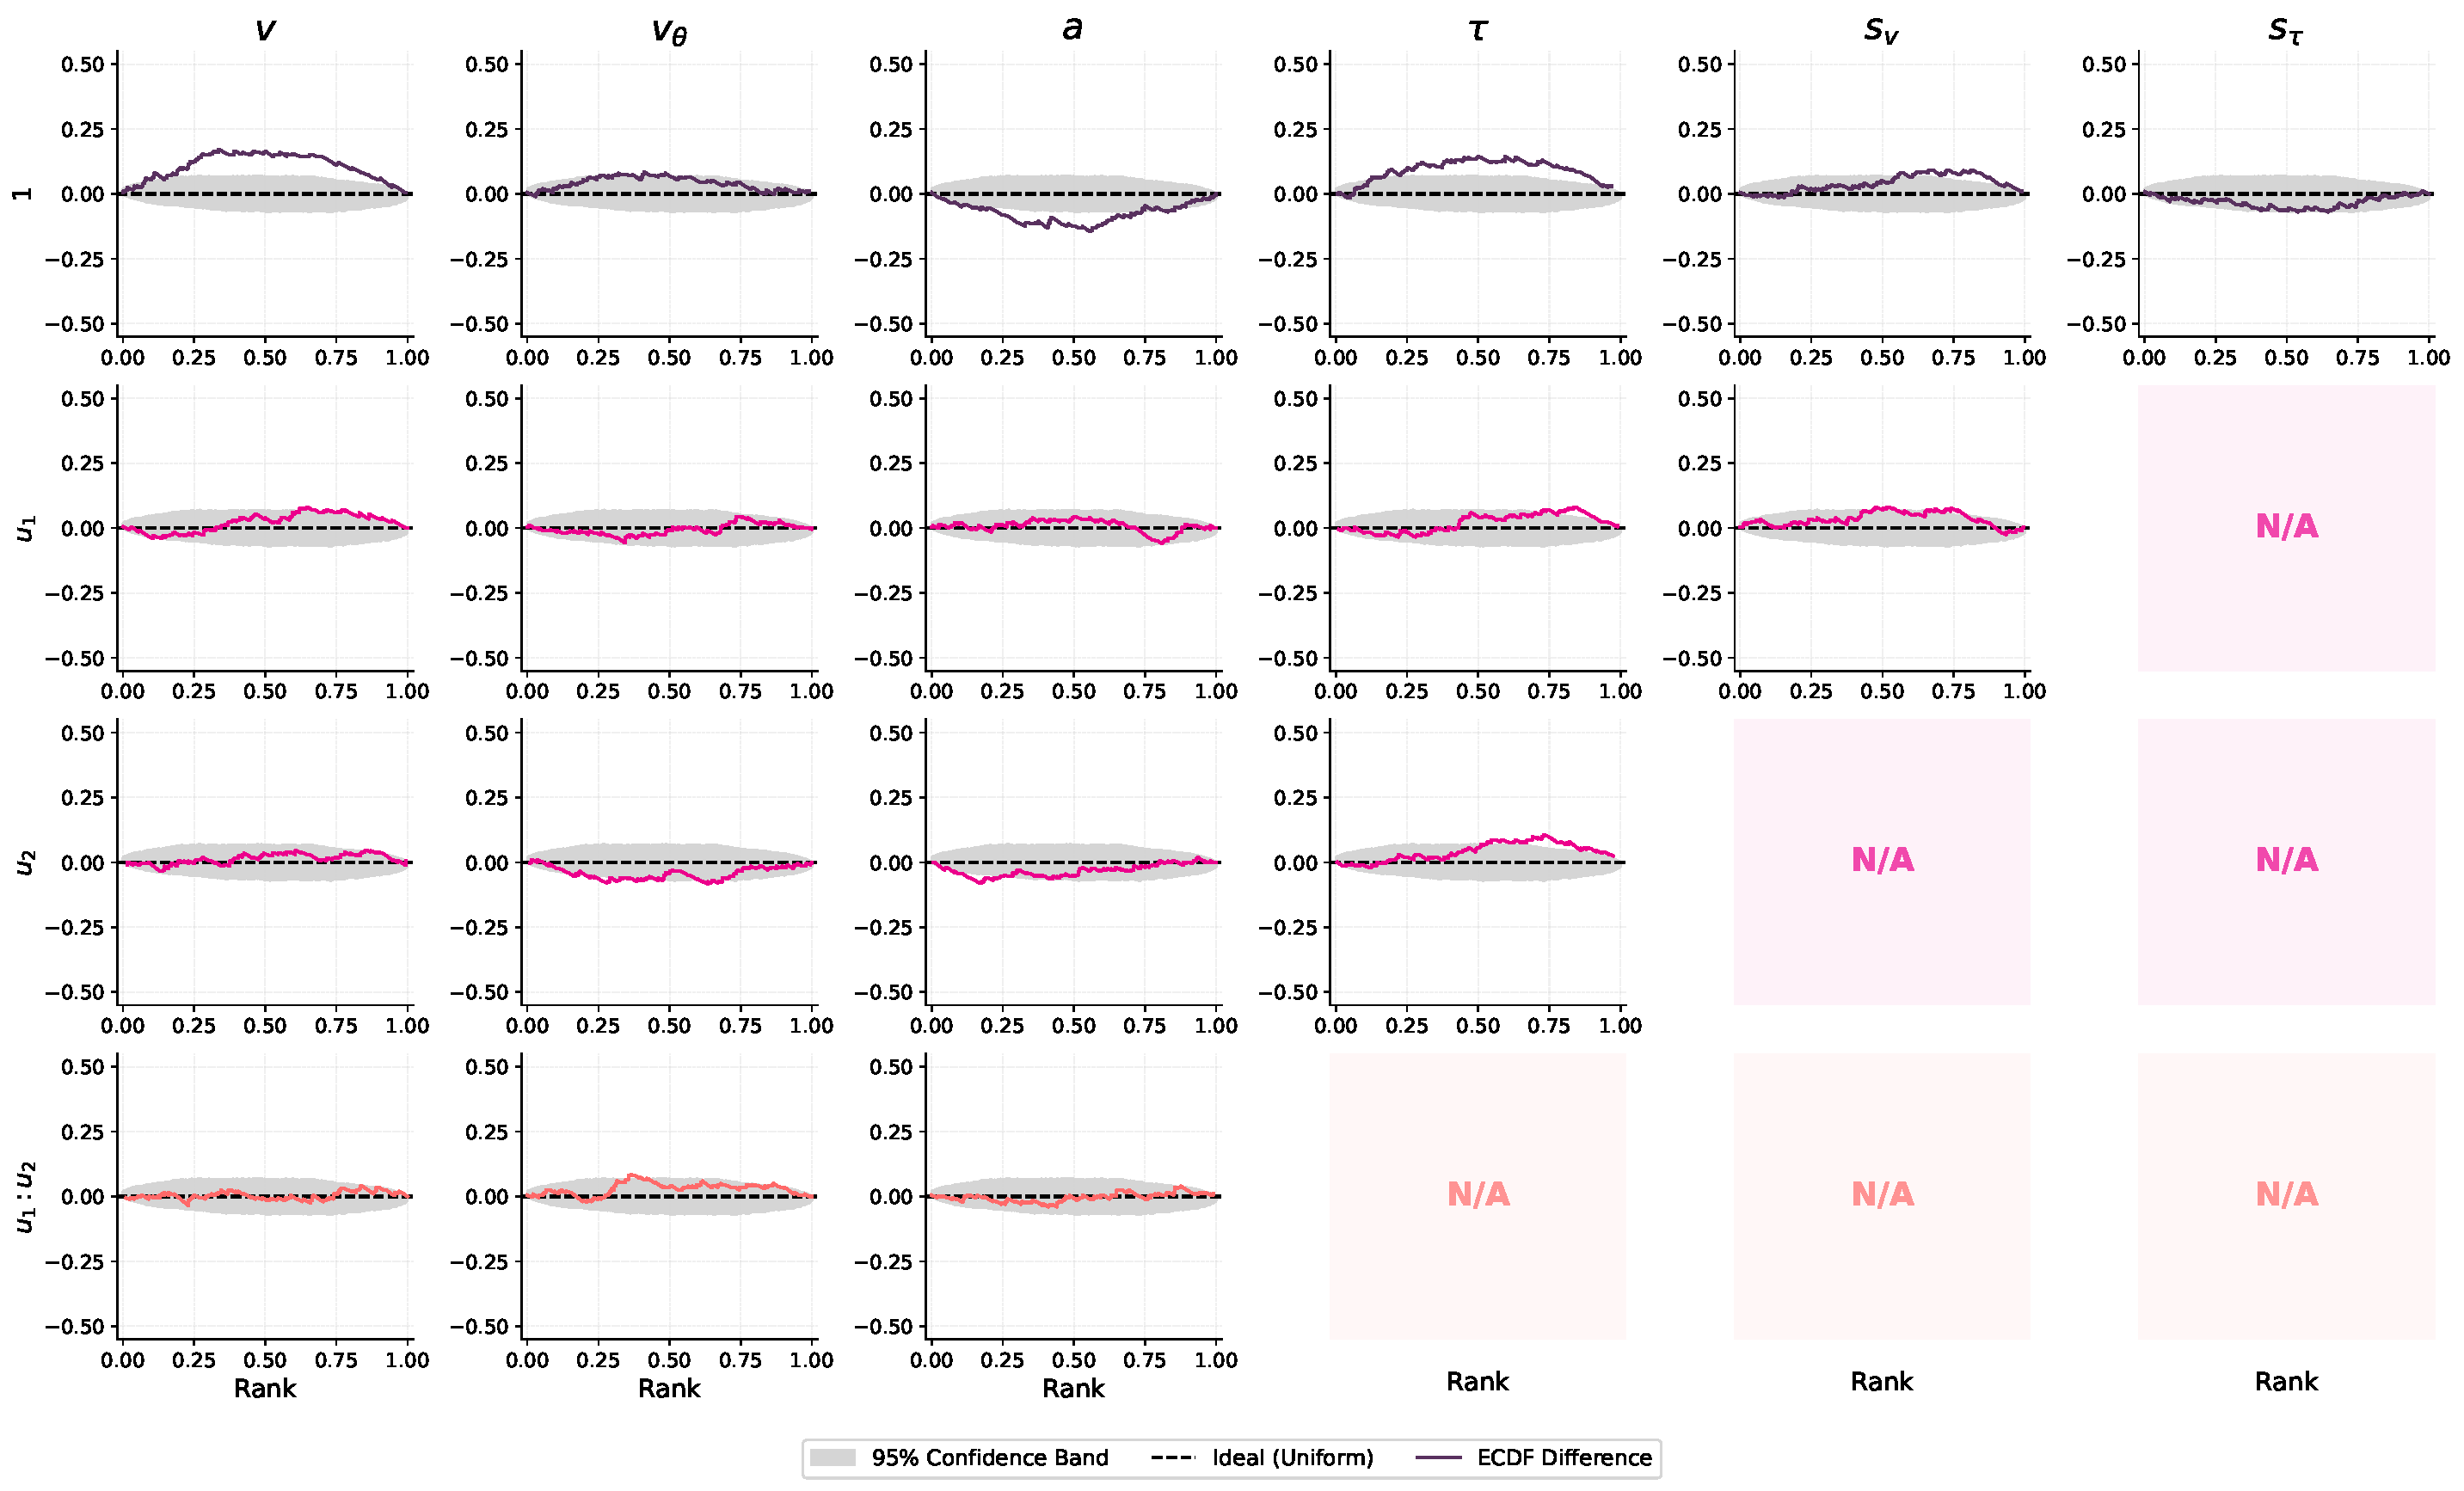
\includegraphics[width=0.99\linewidth]{figures/fm/cdm/interaction/cdm_family_interaction_fm_mixed_ecdf.pdf}
    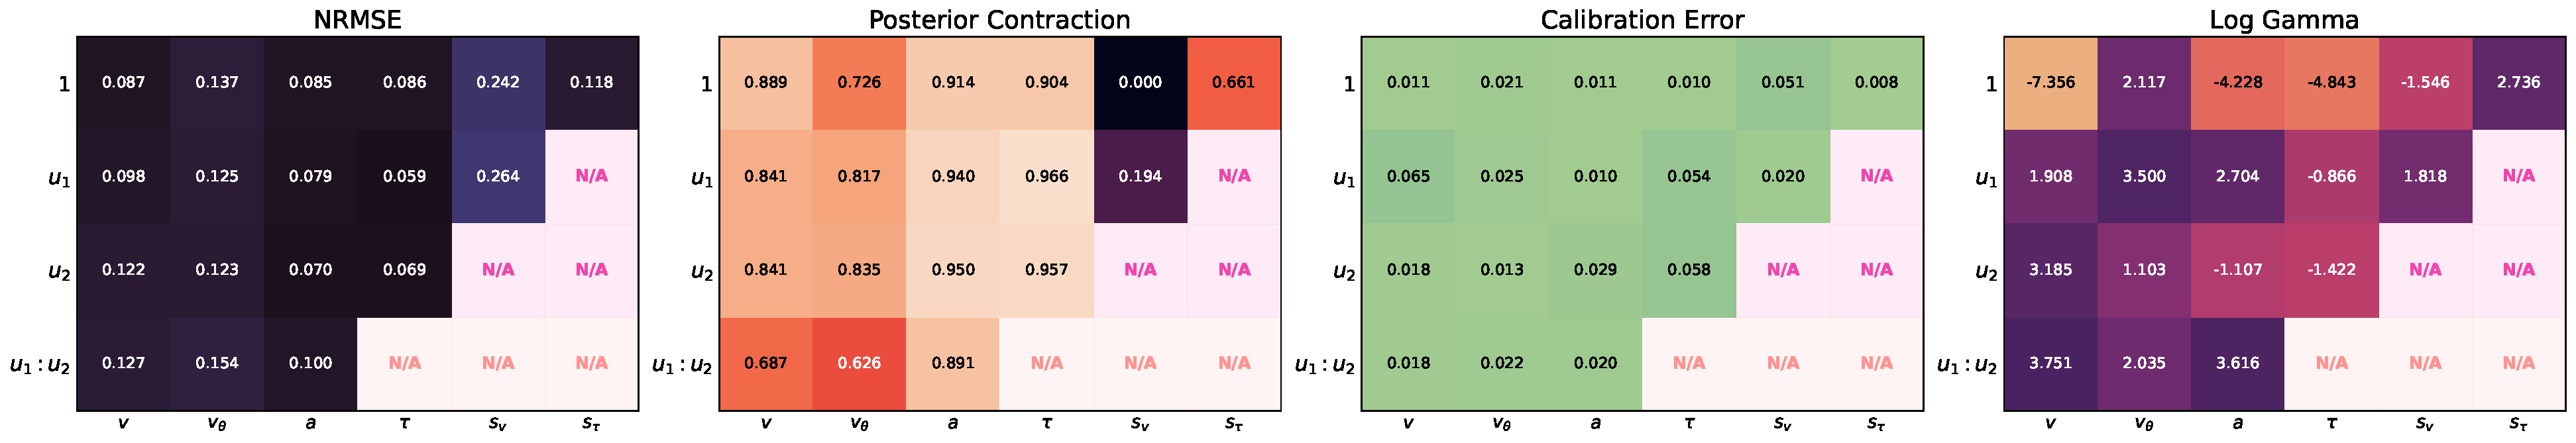
\includegraphics[width=0.99\linewidth]{figures/fm/cdm/interaction/cdm_family_interaction_fm_mixed_metrics.pdf}
    \caption{Parameter recovery (\emph{top}), calibration ECDF (\emph{middle}), and parameter-wise metrics (NRMSE, calibration error, and posterior contraction) for CDM model family (Case \textbf{interaction}).}
    \label{fig:cdm-fm-interaction}
\end{figure}

% ========================================
% DDM MODEL CLASS (mc)
% ========================================

\begin{figure}
    \centering
    \includegraphics[width=0.97\linewidth]{figures/mc/ddm/intercept_only/ddm_family_intercept_only_mc_recovery.pdf}
    \includegraphics[width=0.97\linewidth]{figures/mc/ddm/intercept_only/ddm_family_intercept_only_mc_ecdf.pdf}
    \includegraphics[width=0.97\linewidth]{figures/mc/ddm/intercept_only/ddm_family_intercept_only_mc_metrics.pdf}
    \caption{Parameter recovery (\emph{top}), calibration ECDF (\emph{middle}), and parameter-wise metrics (NRMSE, calibration error, and posterior contraction) for DDM model class (Case \textbf{intercept\_only}).}
    \label{fig:ddm-mc-intercept-only}
\end{figure}

\begin{figure}
    \centering
    \includegraphics[width=0.97\linewidth]{figures/mc/ddm/fixed/ddm_family_fixed_mc_recovery.pdf}
    \includegraphics[width=0.97\linewidth]{figures/mc/ddm/fixed/ddm_family_fixed_mc_ecdf.pdf}
    \includegraphics[width=0.97\linewidth]{figures/mc/ddm/fixed/ddm_family_fixed_mc_metrics.pdf}
    \caption{Parameter recovery (\emph{top}), calibration ECDF (\emph{middle}), and parameter-wise metrics (NRMSE, calibration error, and posterior contraction) for DDM model class (Case \textbf{fixed}).}
    \label{fig:ddm-mc-fixed}
\end{figure}

\begin{figure}
    \centering
    \includegraphics[width=0.97\linewidth]{figures/mc/ddm/regressed/ddm_family_regressed_mc_recovery.pdf}
    \includegraphics[width=0.97\linewidth]{figures/mc/ddm/regressed/ddm_family_regressed_mc_ecdf.pdf}
    \includegraphics[width=0.97\linewidth]{figures/mc/ddm/regressed/ddm_family_regressed_mc_metrics.pdf}
    \caption{Parameter recovery (\emph{top}), calibration ECDF (\emph{middle}), and parameter-wise metrics (NRMSE, calibration error, and posterior contraction) for DDM model class (Case \textbf{regressed}).}
    \label{fig:ddm-mc-regressed}
\end{figure}

\begin{figure}
    \centering
    \includegraphics[width=0.97\linewidth]{figures/mc/ddm/fixed_regressed/ddm_family_fixed_regressed_mc_recovery.pdf}
    \includegraphics[width=0.97\linewidth]{figures/mc/ddm/fixed_regressed/ddm_family_fixed_regressed_mc_ecdf.pdf}
    \includegraphics[width=0.97\linewidth]{figures/mc/ddm/fixed_regressed/ddm_family_fixed_regressed_mc_metrics.pdf}
    \caption{Parameter recovery (\emph{top}), calibration ECDF (\emph{middle}), and parameter-wise metrics (NRMSE, calibration error, and posterior contraction) for DDM model class (Case \textbf{fixed\_regressed}).}
    \label{fig:ddm-mc-fixed-regressed}
\end{figure}

\begin{figure}
    \centering
    \includegraphics[width=0.97\linewidth]{figures/mc/ddm/interaction/ddm_family_interaction_mc_recovery.pdf}
    \includegraphics[width=0.97\linewidth]{figures/mc/ddm/interaction/ddm_family_interaction_mc_ecdf.pdf}
    \includegraphics[width=0.97\linewidth]{figures/mc/ddm/interaction/ddm_family_interaction_mc_metrics.pdf}
    \caption{Parameter recovery (\emph{top}), calibration ECDF (\emph{middle}), and parameter-wise metrics (NRMSE, calibration error, and posterior contraction) for DDM model class (Case \textbf{interaction}).}
    \label{fig:ddm-mc-interaction}
\end{figure}

% ========================================
% RDM MODEL CLASS (mc)
% ========================================

\begin{figure}
    \centering
    \includegraphics[width=0.97\linewidth]{figures/mc/rdm/intercept_only/rdm_family_intercept_only_mc_recovery.pdf}
    \includegraphics[width=0.97\linewidth]{figures/mc/rdm/intercept_only/rdm_family_intercept_only_mc_ecdf.pdf}
    \includegraphics[width=0.97\linewidth]{figures/mc/rdm/intercept_only/rdm_family_intercept_only_mc_metrics.pdf}
    \caption{Parameter recovery (\emph{top}), calibration ECDF (\emph{middle}), and parameter-wise metrics (NRMSE, calibration error, and posterior contraction) for RDM model class (Case \textbf{intercept\_only}).}
    \label{fig:rdm-mc-intercept-only}
\end{figure}

\begin{figure}
    \centering
    \includegraphics[width=0.97\linewidth]{figures/mc/rdm/fixed/rdm_family_fixed_mc_recovery.pdf}
    \includegraphics[width=0.97\linewidth]{figures/mc/rdm/fixed/rdm_family_fixed_mc_ecdf.pdf}
    \includegraphics[width=0.97\linewidth]{figures/mc/rdm/fixed/rdm_family_fixed_mc_metrics.pdf}
    \caption{Parameter recovery (\emph{top}), calibration ECDF (\emph{middle}), and parameter-wise metrics (NRMSE, calibration error, and posterior contraction) for RDM model class (Case \textbf{fixed}).}
    \label{fig:rdm-mc-fixed}
\end{figure}

\begin{figure}
    \centering
    \includegraphics[width=0.97\linewidth]{figures/mc/rdm/regressed/rdm_family_regressed_mc_recovery.pdf}
    \includegraphics[width=0.97\linewidth]{figures/mc/rdm/regressed/rdm_family_regressed_mc_ecdf.pdf}
    \includegraphics[width=0.97\linewidth]{figures/mc/rdm/regressed/rdm_family_regressed_mc_metrics.pdf}
    \caption{Parameter recovery (\emph{top}), calibration ECDF (\emph{middle}), and parameter-wise metrics (NRMSE, calibration error, and posterior contraction) for RDM model class (Case \textbf{regressed}).}
    \label{fig:rdm-mc-regressed}
\end{figure}

\begin{figure}
    \centering
    \includegraphics[width=0.97\linewidth]{figures/mc/rdm/fixed_regressed/rdm_family_fixed_regressed_mc_recovery.pdf}
    \includegraphics[width=0.97\linewidth]{figures/mc/rdm/fixed_regressed/rdm_family_fixed_regressed_mc_ecdf.pdf}
    \includegraphics[width=0.97\linewidth]{figures/mc/rdm/fixed_regressed/rdm_family_fixed_regressed_mc_metrics.pdf}
    \caption{Parameter recovery (\emph{top}), calibration ECDF (\emph{middle}), and parameter-wise metrics (NRMSE, calibration error, and posterior contraction) for RDM model class (Case \textbf{fixed\_regressed}).}
    \label{fig:rdm-mc-fixed-regressed}
\end{figure}

\begin{figure}
    \centering
    \includegraphics[width=0.97\linewidth]{figures/mc/rdm/interaction/rdm_family_interaction_mc_recovery.pdf}
    \includegraphics[width=0.97\linewidth]{figures/mc/rdm/interaction/rdm_family_interaction_mc_ecdf.pdf}
    \includegraphics[width=0.97\linewidth]{figures/mc/rdm/interaction/rdm_family_interaction_mc_metrics.pdf}
    \caption{Parameter recovery (\emph{top}), calibration ECDF (\emph{middle}), and parameter-wise metrics (NRMSE, calibration error, and posterior contraction) for RDM model class (Case \textbf{interaction}).}
    \label{fig:rdm-mc-interaction}
\end{figure}

% ========================================
% CDM MODEL CLASS (mc)
% ========================================

\begin{figure}
    \centering
    \includegraphics[width=0.97\linewidth]{figures/mc/cdm/intercept_only/cdm_family_intercept_only_mc_recovery.pdf}
    \includegraphics[width=0.97\linewidth]{figures/mc/cdm/intercept_only/cdm_family_intercept_only_mc_ecdf.pdf}
    \includegraphics[width=0.97\linewidth]{figures/mc/cdm/intercept_only/cdm_family_intercept_only_mc_metrics.pdf}
    \caption{Parameter recovery (\emph{top}), calibration ECDF (\emph{middle}), and parameter-wise metrics (NRMSE, calibration error, and posterior contraction) for CDM model class (Case \textbf{intercept\_only}).}
    \label{fig:cdm-mc-intercept-only}
\end{figure}

\begin{figure}
    \centering
    \includegraphics[width=0.97\linewidth]{figures/mc/cdm/fixed/cdm_family_fixed_mc_recovery.pdf}
    \includegraphics[width=0.97\linewidth]{figures/mc/cdm/fixed/cdm_family_fixed_mc_ecdf.pdf}
    \includegraphics[width=0.97\linewidth]{figures/mc/cdm/fixed/cdm_family_fixed_mc_metrics.pdf}
    \caption{Parameter recovery (\emph{top}), calibration ECDF (\emph{middle}), and parameter-wise metrics (NRMSE, calibration error, and posterior contraction) for CDM model class (Case \textbf{fixed}).}
    \label{fig:cdm-mc-fixed}
\end{figure}

\begin{figure}
    \centering
    \includegraphics[width=0.97\linewidth]{figures/mc/cdm/regressed/cdm_family_regressed_mc_recovery.pdf}
    \includegraphics[width=0.97\linewidth]{figures/mc/cdm/regressed/cdm_family_regressed_mc_ecdf.pdf}
    \includegraphics[width=0.97\linewidth]{figures/mc/cdm/regressed/cdm_family_regressed_mc_metrics.pdf}
    \caption{Parameter recovery (\emph{top}), calibration ECDF (\emph{middle}), and parameter-wise metrics (NRMSE, calibration error, and posterior contraction) for CDM model class (Case \textbf{regressed}).}
    \label{fig:cdm-mc-regressed}
\end{figure}

\begin{figure}
    \centering
    \includegraphics[width=0.97\linewidth]{figures/mc/cdm/fixed_regressed/cdm_family_fixed_regressed_mc_recovery.pdf}
    \includegraphics[width=0.97\linewidth]{figures/mc/cdm/fixed_regressed/cdm_family_fixed_regressed_mc_ecdf.pdf}
    \includegraphics[width=0.97\linewidth]{figures/mc/cdm/fixed_regressed/cdm_family_fixed_regressed_mc_metrics.pdf}
    \caption{Parameter recovery (\emph{top}), calibration ECDF (\emph{middle}), and parameter-wise metrics (NRMSE, calibration error, and posterior contraction) for CDM model class (Case \textbf{fixed\_regressed}).}
    \label{fig:cdm-mc-fixed-regressed}
\end{figure}

\begin{figure}
    \centering
    \includegraphics[width=0.97\linewidth]{figures/mc/cdm/interaction/cdm_family_interaction_mc_recovery.pdf}
    \includegraphics[width=0.97\linewidth]{figures/mc/cdm/interaction/cdm_family_interaction_mc_ecdf.pdf}
    \includegraphics[width=0.97\linewidth]{figures/mc/cdm/interaction/cdm_family_interaction_mc_metrics.pdf}
    \caption{Parameter recovery (\emph{top}), calibration ECDF (\emph{middle}), and parameter-wise metrics (NRMSE, calibration error, and posterior contraction) for CDM model class (Case \textbf{interaction}).}
    \label{fig:cdm-mc-interaction}
\end{figure}
